\DocumentMetadata{testphase={phase-II,table}, pdfstandard=A-2U, lang=fr-CA}

% Configuration du document
\documentclass[11pt]{book}

% correction pour pandoc 1.14
\providecommand{\tightlist}{%
\setlength{\itemsep}{0pt}\setlength{\parskip}{0pt}}

\usepackage{tabu} % https://tex.stackexchange.com/questions/50332/vertical-spacing-of-a-table-cell

\usepackage{threeparttable}

% Localisation du dépôt csas-style : ajuster le chemin au besoin
\newcommand{\locRepo}{csas-style}
% \usepackage{csas-style}

% Utiliser le fichier de style dans le dépôt csas-style (res-doc.sty)
% \usepackage{\locRepo/res-doc}
\usepackage{./csas-style/res-doc}

% header-includes de l'entrée R markdown

% En-têtes et pieds de page
\lhead{Ébauche de document de travail --- Ne pas citer ou diffuser}
% \lhead{}
\rhead{}
% \rfoot{ÉBAUCHE - NE PAS CITER}

% Améliorations d'accessibilité visuelle
\usepackage{environ}
\NewEnviron{taggedfigure}[3]{%
  % \tagstructbegin{tag=Figure,alttext={#1}}%
  \tagstructbegin{tag=Figure,alttext=Figure}%
  \tagmcbegin{tag=Figure}%
  {\centering \includegraphics[width=#2]{#3}}%
  \tagmcend%
  \tagstructend%
  \tagpdfparaOn%
  \tagstructbegin{tag=Caption}%
  \tagmcbegin{tag=Caption}%
  \BODY%
  \tagmcend%
  \tagstructend%
}

%%%% Commandes pour la page de titre etc %%%%%

% Année de publication
\newcommand{\rdYear}{2024}

% Mois de publication
\newcommand{\rdMonth}{Mois}

% Numéro du rapport
\newcommand{\rdNumber}{nnn}

% Région
\newcommand{\rdRegion}{Région du Pacifique}

% Titre
\newcommand{\rdTitle}{Sélectivité des proies de l'épaulard résident du Sud en relation avec la composition des stocks et de la taille du saumon chinook dans l'habitat essentiel canadien}

\newcommand{\rdISBN}{978-0-660-38322-4}
\newcommand{\rdCatNo}{Fs70-6/2021-012F-PDF}

% Noms des auteurs séparés par des virgules et ', et' pour le dernier auteur au format 'M.H. Grinnell' (utiliser \textsuperscript{n} pour les adresses)
\newcommand{\rdAuth}{
Cameron Freshwater\textsuperscript{1}, Wilf Luedke\textsuperscript{1}, Scott Toews\textsuperscript{2}, et Sheila J. Thornton\textsuperscript{2}}

% Noms des auteurs inversés séparés par des virgules au format 'Grinnell, M.H.'
\newcommand{\rdAuthRev}{
Freshwater, C., Luedke, W., Toews, S., Thornton, S.}

% Adresses des auteurs (utiliser \textsuperscript{n})
\newcommand{\rdAuthAddy}{
\textsuperscript{1}Station biologique du Pacifique\\
Pêches et Océans Canada, 3190 Hammond Bay Road\\
Nanaimo, Colombie-Britannique, V9T 6N7, Canada\\
\smallskip \textsuperscript{2}Centre d'entreprise scientifique du Pacifique\\
Pêches et Océans Canada, 4160 Marine Drive\\
West Vancouver, Colombie-Britannique, V7V 1H2, Canada\\
}

\newcommand{\citationOtherLanguage}{Last, F.M. and Smith, A.B. Title Here (\emph{Latin Species Name}). DFO Can. Sci. Advis. Sec. Res. Doc. 2019/nnn. iv + 13 p.}

% \linenumbers

% Packages français pour la typographie
\usepackage[french]{babel}
\usepackage[T1]{fontenc}
\usepackage{lmodern}

\newcommand{\rdAbstract}{\abstract{
Deux populations d'un écotype d'épaulard piscivore (\textit{Orcinus orca}) vivent dans les eaux canadiennes du Pacifique : les épaulards résidents du Nord et du Sud. Ces populations sont respectivement inscrites comme menacées et en voie de disparition en vertu de la \textit{Loi sur les espèces en péril} du Canada. Le saumon chinook (\textit{Oncorhynchus tschawytscha}) constitue une proie clé pour les deux populations et le déclin de la disponibilité des proies est un facteur probable limitant le rétablissement des épaulards résidents. L'habitat essentiel de l'épaulard résident du Sud (ÉRES) du Canada a été identifié dans la mer des Salish. Cette région abrite également un large éventail de populations de saumon chinook aux histoires de vie, caractéristiques physiques et tendances d'abondance diverses. Ce rapport résume les patrons saisonniers et spatiaux de l'abondance relative de 11 stocks de saumon chinook et de quatre classes de taille dans l'habitat essentiel de l'ÉRES au Canada, en mettant l'accent sur les mois d'été et les zones s'étendant du détroit ouest de Juan de Fuca aux îles Gulf du Sud. Les données de composition des stocks et des âges du saumon chinook provenant des restes de proies de l'ÉRES (2007-2023) ont été évaluées, ainsi que les estimations basées sur des modèles de la composition de la taille des proies. Un deuxième ensemble de données d'échantillons provenant de pêches récréatives au saumon chinook, collectés entre 2014 et 2023, a été utilisé pour paramétrer des modèles géostatistiques qui ont fourni un indice du champ de proies. Les deux ensembles de données ont ensuite été comparés pour tester l'évidence de la sélectivité de l'alimentation de l'ÉRES. Enfin, ces résultats ont été évalués dans le contexte de l'amélioration de l'écloserie au Canada, ainsi que des différences entre les stocks de saumon chinook en matière de caractéristiques biologiques et de tendances de l'abondance terminale.

Bien que tous les stocks de saumon chinook aient été observés dans les restes de proies de l'ÉRES, les stocks Fraser River Spring $5_2$ et Summer $4_1$ étaient les plus communs. Indépendamment de l'identité du stock, les saumons chinook relativement plus âgés étaient plus communs dans les restes de proies de l'ÉRES que les individus plus jeunes. Les prédictions d'un modèle de taille selon l'âge spécifique à la saison et au stock indiquaient que les restes de proies provenaient principalement de poissons de plus de 75 cm de longueur à la fourche. Selon l'emplacement et la semaine, les saumons chinook Columbia River Summer/Fall, Puget Sound, côte ouest de l'île de Vancouver (COIV), et Fraser River Summer $4_1$ figuraient parmi les stocks les plus abondants dans les échantillons dépendants de la pêche. Les deux plus grandes classes de taille de saumon chinook étaient les plus abondantes en juillet et août et dans les emplacements près de Port Renfrew. Une analyse de simulation comparant les prédictions du modèle géostatistique dépendant de la pêche aux restes de proies observés a trouvé des preuves mitigées de sélectivité des proies par l'ÉRES. Les stocks Fraser River Spring $5_2$, Summer $5_2$, et Summer $4_1$ se produisaient plus fréquemment qu'attendu dans les restes de proies tandis que les stocks COIV, Puget Sound, Columbia River Summer/Fall, et divers (c.-à-d., « Autre ») se produisaient moins fréquemment qu'attendu. Les stocks restants étaient présents dans les proies approximativement proportionnellement à leur abondance telle que prédite par le modèle dépendant de la pêche. Les deux plus petites classes de taille de saumon chinook ($55-65$ cm et $65-75$ cm de longueur à la fourche) étaient sous-représentées dans les restes de proies de l'ÉRES, tandis que les plus grandes classes de taille ($65-75$ et $75-85$ cm) étaient sur-représentées. Les saumons d'origine d'écloserie canadienne ont été identifiés dans les restes de proies de l'ÉRES en utilisant le PBT ; cependant, ces estimations sont probablement biaisées vers le bas en raison de la couverture incomplète du PBT pendant la période d'échantillonnage. Aucun des stocks qui ont montré des preuves de sélectivité positive n'est fortement amélioré, tandis que les stocks Puget Sound et COIV, qui sont fortement améliorés, ont été sélectionnés négativement. Cependant, les poissons d'origine d'écloserie peuvent être des éléments de proie importants dans d'autres emplacements ou périodes. L'abondance terminale, sommée sur tous les stocks de saumon chinook présents dans l'habitat essentiel canadien, n'a pas diminué ; cependant, les stocks ont montré des tendances divergentes d'abondance. En particulier, les stocks Fraser River Spring $4_2$, Spring $5_2$, et Summer $5_2$ ont diminué, tandis que les stocks Fraser River Summer $4_1$, côte est de l'île de Vancouver, et COIV ont augmenté.

Les ÉRES dépendent d'un assemblage diversifié de saumons chinook dont la disponibilité des stocks et des classes de taille varie à fine échelle, saisonnièrement et spatialement. Cependant, les saumons chinook de grande taille et riches en énergie sont probablement des proies clés, particulièrement pendant le printemps et le début de l'été lorsque l'ÉRES peut être en condition physique relativement pauvre. Les interventions de gestion qui augmentent la disponibilité de saumons chinook de grande taille ou à haute teneur en lipides pendant cette période peuvent être particulièrement importantes pour le rétablissement de l'ÉRES. Les augmentations pourraient se produire en reconstruisant les stocks de saumon chinook actuellement épuisés avec ces traits (p. ex., Fraser Spring $5_2$, Fraser Summer $5_2$) ou en augmentant la taille moyenne individuelle ou la teneur en lipides des stocks actuellement abondants qui se chevauchent dans l'espace et le temps avec les habitats d'alimentation de l'ÉRES.
}}

%%%% Fin des commandes de page de titre %%%%%

% \pdfcompresslevel=5 % PNGs plus rapides

\setcounter{section}{0}

% \bibliographystyle{csas-style/res-doc}

\usepackage{amsmath}
\usepackage{bm}

% commandes et environnements nécessaires pour les extraits pandoc
% extraits de la sortie de `pandoc -s`
%% Faire fonctionner les blocs de code R markdown
\usepackage{array}
\usepackage{amssymb,amsmath}
\usepackage{color}
\usepackage{fancyvrb}

% Du modèle par défaut :
\newcommand{\VerbBar}{|}
\newcommand{\VERB}{\Verb[commandchars=\\\{\}]}
\DefineVerbatimEnvironment{Highlighting}{Verbatim}{commandchars=\\\{\},formatcom=\color[rgb]{0.00,0.00,0.00}}
\usepackage{framed}
\definecolor{shadecolor}{RGB}{248,248,248}
\newenvironment{Shaded}{\begin{snugshade}}{\end{snugshade}}
\newcommand{\AlertTok}[1]{\textcolor[rgb]{0.94,0.16,0.16}{#1}}
\newcommand{\AnnotationTok}[1]{\textcolor[rgb]{0.56,0.35,0.01}{\textbf{\textit{#1}}}}
\newcommand{\AttributeTok}[1]{\textcolor[rgb]{0.77,0.63,0.00}{#1}}
\newcommand{\BaseNTok}[1]{\textcolor[rgb]{0.00,0.00,0.81}{#1}}
\newcommand{\BuiltInTok}[1]{#1}
\newcommand{\CharTok}[1]{\textcolor[rgb]{0.31,0.60,0.02}{#1}}
\newcommand{\CommentTok}[1]{\textcolor[rgb]{0.56,0.35,0.01}{\textbf{#1}}}
\newcommand{\CommentVarTok}[1]{\textcolor[rgb]{0.56,0.35,0.01}{\textbf{\textit{#1}}}}
\newcommand{\ConstantTok}[1]{\textcolor[rgb]{0.00,0.00,0.00}{#1}}
\newcommand{\ControlFlowTok}[1]{\textcolor[rgb]{0.13,0.29,0.53}{\textit{#1}}}
\newcommand{\DataTypeTok}[1]{\textcolor[rgb]{0.13,0.29,0.53}{#1}}
\newcommand{\DecValTok}[1]{\textcolor[rgb]{0.00,0.00,0.81}{#1}}
\newcommand{\DocumentationTok}[1]{\textcolor[rgb]{0.56,0.35,0.01}{\textbf{\textit{#1}}}}
\newcommand{\ErrorTok}[1]{\textcolor[rgb]{0.64,0.00,0.00}{\textit{#1}}}
\newcommand{\ExtensionTok}[1]{#1}
\newcommand{\FloatTok}[1]{\textcolor[rgb]{0.00,0.00,0.81}{#1}}
\newcommand{\FunctionTok}[1]{\textcolor[rgb]{0.00,0.00,0.00}{#1}}
\newcommand{\ImportTok}[1]{#1}
\newcommand{\InformationTok}[1]{\textcolor[rgb]{0.56,0.35,0.01}{\textbf{\textit{#1}}}}
\newcommand{\KeywordTok}[1]{\textcolor[rgb]{0.13,0.29,0.53}{\textit{#1}}}
\newcommand{\NormalTok}[1]{#1}
\newcommand{\OperatorTok}[1]{\textcolor[rgb]{0.81,0.36,0.00}{\textit{#1}}}
\newcommand{\OtherTok}[1]{\textcolor[rgb]{0.56,0.35,0.01}{#1}}
\newcommand{\PreprocessorTok}[1]{\textcolor[rgb]{0.56,0.35,0.01}{\textbf{#1}}}
\newcommand{\RegionMarkerTok}[1]{#1}
\newcommand{\SpecialCharTok}[1]{\textcolor[rgb]{0.00,0.00,0.00}{#1}}
\newcommand{\SpecialStringTok}[1]{\textcolor[rgb]{0.31,0.60,0.02}{#1}}
\newcommand{\StringTok}[1]{\textcolor[rgb]{0.31,0.60,0.02}{#1}}
\newcommand{\VariableTok}[1]{\textcolor[rgb]{0.00,0.00,0.00}{#1}}
\newcommand{\VerbatimStringTok}[1]{\textcolor[rgb]{0.31,0.60,0.02}{#1}}
\newcommand{\WarningTok}[1]{\textcolor[rgb]{0.56,0.35,0.01}{\textbf{\textit{#1}}}}

\newcommand{\lt}{\ensuremath <}
\newcommand{\gt}{\ensuremath >}

%Définit l'environnement cslreferences
%Requis par pandoc 2.8
%Copié de https://github.com/rstudio/rmarkdown/issues/1649
% % \newlength{\cslhangindent}
% \setlength{\cslhangindent}{1.5em}
% \newenvironment{cslreferences}%
%   {}%
%   {\par}
% 

\DeclareGraphicsExtensions{.png,.pdf}

%%%%%%%%%%%%%%%%%
% éléments ajoutés
\usepackage[round]{natbib}
\bibliographystyle{res-doc}
\bibpunct{(}{)}{,}{a}{}{,}
% \renewcommand{\bibname}{RÉFÉRENCES CITÉES}
\addto{\extrasfrench}{%
  \renewcommand{\bibname}{RÉFÉRENCES CITÉES}
}
\newcommand{\note}[1]{{\color{red}#1}}
%%%%%%%%%%%%%%%%%

\begin{document}

\frontmatter

\section{INTRODUCTION}\label{sec:introduction}

Les eaux canadiennes du Pacifique abritent trois écotypes d'épaulards (\textit{Orcinus orca}), chacun génétiquement distinct et présentant des différences significatives en morphologie, comportement et alimentation. L'écotype résident piscivore comprend deux populations — l'épaulard résident du Nord (ÉREN) et l'épaulard résident du Sud (ÉRES). Le saumon du Pacifique (\textit{Oncorhynchus} spp.) forme une grande partie de leur alimentation, le saumon chinook (\textit{O. tshawytscha}) étant identifié comme l'espèce proie dominante \citep{fordSelectiveForagingFisheating2006, fordDietarySpecializationTwo1998, hansonSpeciesStockIdentification2010}. De 1962 à 1973, les deux populations résidentes ont subi des prélèvements importants en raison de la pêche de capture vivante \citep{biggLivecaptureKillerWhale1975}. Un recensement annuel a lieu depuis la fermeture de la pêcherie, les données récentes indiquant que la population d'ÉREN continue de présenter une augmentation annuelle de 2,5 à 3,5\% et compte approximativement 341 individus \citep{dfoPopulationStatusUpdate2023}. La population d'ÉRES a échoué à maintenir une trajectoire de croissance positive et ne consiste qu'en 74 individus. Les populations sont inscrites en vertu de la \textit{Loi sur les espèces en péril} comme menacées et en voie de disparition, respectivement \citep{cosewicCOSEWICAssessmentUpdate2001, cosewicCOSEWICAssessmentStatus2023}.

La distribution de l'ÉRES s'étend de la Californie centrale au sud-est de l'Alaska \citep{thorntonSouthernResidentKiller2022}. Pendant les mois d'été, l'ÉRES utilisait historiquement de manière extensive la mer des Salish, qui comprend le détroit de Georgie, le détroit d'Haro, Puget Sound, et le détroit de Juan de Fuca \citep{fordSelectiveForagingFisheating2006, fordHabitatsSpecialImportance2017}. Plus récemment, les zones à l'ouest du détroit de Juan de Fuca, y compris le banc de La Perouse, le banc Swiftsure, et les canyons sous-marins proximaux ont été identifiés comme habitat essentiel pendant l'été ainsi qu'en hiver \citep{fordHabitatsSpecialImportance2017, thorntonSouthernResidentKiller2022}. L'utilisation de l'habitat par l'ÉRES est associée aux migrations du saumon du Pacifique, et en particulier du saumon chinook, qui se trouvent dans la mer des Salish et les eaux associées du plateau continental toute l'année \citep{oneillMarineDistributionLife2009, chamberlinEffectsNatalOrigin2014, freshwaterIntegratedModelSeasonal2021}.

Un des plusieurs facteurs hypothétiques des faibles taux de croissance de la population chez l'ÉRES est la disponibilité réduite des proies, avec un accent particulier sur les déclins de l'abondance du saumon chinook. Les observations des régimes alimentaires de l'ÉRES sont typiquement dominées par le saumon chinook, bien que la diversité des proies augmente en hiver pour inclure le saumon coho (\textit{O. kisutch}), le saumon kéta (\textit{O. keta}), et la morue charbonnière (\textit{Anoplopoma fimbria}) \citep{fordLinkingKillerWhale2010, fordEstimationKillerWhale2016, hansonEndangeredPredatorsEndangered2021}. De plus, les taux démographiques de l'ÉRES covariaient avec les indices à grande échelle de l'abondance du saumon chinook \citep{wardIncreasedPopulationDensity2009, fordLinkingKillerWhale2010}, bien que ces effets se soient avérés difficiles à estimer avec précision étant donné la longue durée de vie des épaulards \citep{velez-espinoRelativeImportanceChinook2015}. Les indices de l'abondance du saumon chinook étaient également corrélés avec les changements de condition individuelle de l'ÉRES \citep{stewartSurvivalFattestLinking2021}, les changements de comportement d'alimentation \citep{holtEffectsVesselDistance2021}, l'utilisation des habitats de la mer des Salish \citep{ettingerShiftingPhenologyEndangered2022, stewartTraditionalSummerHabitat2023}, et, via des modèles d'écosystème équilibrés en masse, les déficits caloriques dans la population d'ÉRES \citep{coutureRequirementsAvailabilityPrey2022}. Néanmoins, certaines preuves suggèrent que les relations entre les taux démographiques de l'ÉRES et l'abondance du chinook se sont affaiblies dans le temps, peut-être en raison de la compétition avec les épaulards résidents du Nord, qui ont augmenté en abondance \citep{nelsonIdentifyingDriversDemographic2024}, ou de l'effet accru d'autres impacts anthropiques sur la santé individuelle (p. ex., mobilisation de contaminants à partir des réserves lipidiques ; facteurs de stress physiologiques tels que les perturbations physiques et acoustiques).

Évaluer les besoins en proies de l'ÉRES, et adapter les interventions de gestion pour répondre à ces besoins, est difficile étant donné la diversité écologique du saumon chinook. Le saumon chinook, comme la plupart des saumons du Pacifique, est anadrome et sémelpare, mais diffère de ses congénères de plusieurs façons notables. Le saumon chinook a la distribution la plus étendue des saumons du Pacifique dans le Pacifique oriental, s'étendant du fleuve Yukon à la Californie centrale. Il présente des stratégies d'histoire de vie diverses pendant l'élevage en eau douce (moins d'un à plusieurs années) et marin (moins d'un à plus de cinq années). En raison de leur âge moyen relativement âgé à la maturité et de leur régime marin principalement piscivore, le saumon chinook atteint la plus grande taille corporelle des saumons du Pacifique et peut dépasser 15 kilogrammes \citep{healeyLifeHistoryChinook1991}.

Le saumon chinook montre une forte fidélité au site de frai et au calendrier de migration, résultant en de nombreuses populations génétiquement distinctes \citep{healeyLifeHistoryChinook1991, quinnBehaviourEcologyPacific2018}. Les populations de saumon chinook peuvent différer selon plusieurs dimensions écologiques incluant la stratégie d'histoire de vie juvénile (c.-à-d., entrant dans l'océan avec (yearling) ou sans (subyearling) hivernage comme juvéniles en eau douce), la phénologie de migration en eau douce des adultes (c.-à-d., calendrier de remontée printanière, estivale, ou automnale), et la distribution marine. Contrairement à de nombreuses espèces de saumons du Pacifique, un nombre substantiel de populations de saumon chinook, principalement des individus subyearling de remontée automnale, passent toute leur vie marine dans les eaux côtières relativement proches de leurs lieux d'entrée océanique \citep{oneillMarineDistributionLife2009, chamberlinEffectsNatalOrigin2014, freshwaterIntegratedModelSeasonal2021}. D'autres populations de remontée estivale et automnale, ainsi que certaines populations yearling, migrent vers le nord sur des distances considérables, mais demeurent sur le plateau continental \citep{weitkampMarineDistributionsChinook2010, ctc2021AnnualReport2022}. Les populations yearling de remontée printanière qui frayent dans les parties intérieures de grands bassins versants se dispersent typiquement au large \citep{weitkampMarineDistributionsChinook2010, ctc2021AnnualReport2022}.

De nombreux stocks de saumon chinook (utilisé tout au long pour faire référence à une ou plusieurs populations de frai distinctes) ont décliné en abondance au cours des 50 dernières années coïncidant avec la surpêche, la perte d'habitat, et les changements de productivité. Dans toute la Californie, les déclins de l'habitat d'eau douce et les conditions environnementales changeantes ont résulté en des réductions substantielles de la diversité des histoires de vie et des pêcheries moins résilientes \citep{munschOneHundredseventyYears2022}. Dans le bassin versant du fleuve Columbia, cinq des sept unités évolutionnaires significatives (UES) sont inscrites comme menacées ou en voie de disparition sous l'Endangered Species Act \citep{nmfsEndangeredSpeciesAct2020}. L'UES du saumon chinook de Puget Sound demeure également inscrite comme menacée \citep{fordStatusReviewUpdate2011}. Dans le sud de la Colombie-Britannique, la majorité des unités de conservation (UC) de saumon chinook évaluées ont été identifiées comme menacées ou en voie de disparition \citep{cosewicChinookSalmonOncorhynchus2018}. Notamment, les déclins se sont produits malgré des investissements considérables dans la remédiation de l'habitat \citep{jaegerReturnsInvestmentRestoration2023} et des réductions des taux d'exploitation \citep{ctc2021AnnualReport2022}. L'étendue spatiale large des déclins, incluant dans les régions avec des habitats d'eau douce relativement vierges, a mené à un consensus scientifique croissant que la faible survie marine et les réductions de l'âge à la maturité ont réduit la productivité et contraint le rétablissement \citep{dornerSpatialTemporalPatterns2017, ruffSalishSeaChinook2017, ohlbergerDemographicChangesChinook2018, welchSynthesisCoastwideDecline2021, freshwaterNonstationaryPatternsDemographic2022}.

Néanmoins, les déclins de l'abondance du saumon chinook ne sont pas uniformes. Les déclins de l'abondance des stocks yearling de remontée printanière dans les grands bassins versants ont été particulièrement sévères, mais plusieurs stocks subyearling de remontée estivale qui frayent dans l'intérieur des mêmes bassins versants ont augmenté en abondance \citep{cosewicChinookSalmonOncorhynchus2018, ctc2021AnnualReport2022, atlasTrendsChinookSalmon2023}. Les tendances de l'abondance des stocks côtiers de remontée automnale sont mitigées avec certains stocks, même dans la même région géographique, augmentant tandis que d'autres déclinent \citep{ctc2021AnnualReport2022, atlasTrendsChinookSalmon2023}. En raison de ces patrons divergents, l'abondance du saumon chinook peut être relativement stable, en augmentation, ou en diminution selon les stocks considérés. Par exemple, puisque les stocks subyearling de remontée estivale et automnale sont abondants relativement aux stocks de remontée printanière, spécialement étant donné la production substantielle d'écloserie, l'abondance agrégée du saumon chinook dans les zones marines s'étendant du sud-est de l'Alaska à l'île de Vancouver est demeurée relativement stable au cours des 30 dernières années \citep{ctc2021AnnualReport2022}. La variabilité parmi les stocks de saumon chinook dans les tendances d'abondance, avec la puissance statistique modeste, peut contribuer aux relations incertaines ou s'affaiblissant entre les estimations grossières de l'abondance du saumon chinook et les taux démographiques de l'ÉRES \citep{nelsonIdentifyingDriversDemographic2024}.

Toutes choses étant égales par ailleurs, les stocks de saumon chinook plus abondants devraient être des composantes plus prévalentes du régime alimentaire de l'ÉRES. Cependant, la contribution de différents stocks de saumon chinook à la base de proies de l'ÉRES peut covarier avec les caractéristiques écologiques. Premièrement, le calendrier de migration du saumon chinook déterminera quand des stocks de saumon spécifiques sont abondants dans les régions, telles que la partie ouest du détroit de Juan de Fuca, où l'ÉRES s'alimente de manière disproportionnée \citep{thorntonSouthernResidentKiller2022}. L'ÉRES montre des patrons saisonniers de condition, indiquant qu'il peut éprouver des limitations de proies avant les observations en mai (Fearnbach et al. 2020; J. Durban, comm. pers.). Une diminution générale de la condition corporelle pendant les mois d'hiver suggère que les stocks de saumon chinook de remontée précoce (c.-à-d., de remontée printanière et estivale précoce) peuvent fournir une ressource critique. En effet, l'utilisation des habitats de la mer des Salish par l'ÉRES s'est produite plus tard dans l'année coïncidant avec les déclins de l'abondance du saumon chinook de remontée printanière du fleuve Fraser et les augmentations de l'abondance des stocks avec un calendrier de migration plus tardif \citep{ettingerShiftingPhenologyEndangered2022}. Deuxièmement, les distributions marines spécifiques aux stocks interagissent avec le calendrier de remontée pour déterminer l'étendue à laquelle des stocks spécifiques de saumon chinook se chevauchent spatialement et temporellement avec l'ÉRES. Alors que de nombreux stocks de saumon chinook ne sont présents dans les zones côtières du sud de la Colombie-Britannique qu'immédiatement avant les migrations de frai, d'autres sont résidents pour toute leur histoire de vie marine et sont disponibles comme proies pour l'ÉRES toute l'année \citep{oneillMarineDistributionLife2009, chamberlinEffectsNatalOrigin2014, freshwaterIntegratedModelSeasonal2021}. Troisièmement, les stocks de saumon chinook diffèrent en âge à la maturité \citep{healeyLifeHistoryChinook1991, ohlbergerDemographicChangesChinook2018}, taille selon l'âge \citep{ohlbergerDemographicChangesChinook2018, xuClimateEffectsSize2020}, et contenu lipidique \citep{oneillEnergyContentPacific2014, lernerSeasonalVariationLipid2023, freshwaterSeasonalVariabilityCondition2024}, qui déterminent collectivement leur valeur énergétique relative. Il est possible que l'ÉRES sélectionne des éléments de proie plus grands ou plus riches en énergie de manière disproportionnée à leur abondance. En effet, les individus de saumon chinook plus grands et plus âgés semblent être plus communs dans les régimes alimentaires des épaulards résidents que dans les pêcheries proximales \citep{fordSelectiveForagingFisheating2006}.

Déterminer la valeur relative des stocks de saumon chinook pour les ÉRES fournit un aperçu des emplacements et des moments où l'ÉRES peut être le plus sensible aux réductions de la disponibilité des proies. Un sous-ensemble de stocks de saumon chinook « de haute valeur » peut fournir un signal écologique plus fort reliant les traits démographiques de l'ÉRES et la condition individuelle à l'abondance des proies. Évaluer la valeur relative des stocks de saumon chinook permet également aux gestionnaires de ressources de prioriser les interventions de gestion qui sont les plus susceptibles d'améliorer la disponibilité des stocks de haute valeur. Alors que la recherche précédente a déterminé que la contribution relative des stocks de saumon chinook aux régimes alimentaires de l'ÉRES varie saisonnièrement \citep{hansonSpeciesStockIdentification2010, hansonEndangeredPredatorsEndangered2021}, les données de composition des proies n'ont pas été directement comparées au champ de proies de fond.

Ici, nous utilisons de multiples lignes de preuves pour évaluer la contribution relative de différents stocks et classes de taille de saumon chinook aux régimes alimentaires de l'ÉRES dans le sud de la Colombie-Britannique. Nous notons qu'en raison des limitations de données, notre analyse se concentre sur les interactions du saumon chinook de l'ouest du détroit de Juan de Fuca au sud du détroit de Georgie pendant les mois d'été (mai-octobre) et n'est pas une évaluation complète des besoins en proies. Néanmoins, la région a été identifiée comme habitat essentiel pour l'ÉRES \citep{dfoIdentificationHabitatsSpecial2017} et la condition des individus ÉRES est corrélée avec les opportunités d'alimentation dans ces zones \citep{ettingerShiftingPhenologyEndangered2022, stewartSurvivalFattestLinking2021, stewartTraditionalSummerHabitat2023}. Premièrement, nous avons utilisé des échantillons de débris de proies pour évaluer la composition des stocks et de la taille des événements d'alimentation de l'ÉRES dans différentes parties de l'habitat essentiel de l'ÉRES. Deuxièmement, nous avons utilisé des échantillons collectés des pêcheries récréatives comme un indice de la disponibilité relative de différents stocks et classes de taille de saumon chinook pour l'ÉRES. Nous avons utilisé des modèles spatio-temporels ajustés aux données dépendantes de la pêcherie pour prédire la composition des stocks et la composition de la taille à des intervalles hebdomadaires à travers l'habitat essentiel de l'ÉRES. Troisièmement, nous avons conduit une analyse de simulation pour déterminer si les échantillons de proies observés déviaient des prédictions dérivées du modèle pour tester l'évidence de la sélection par l'ÉRES de stocks ou de classes de taille de manière disproportionnée à leur abondance. Quatrièmement, nous avons colligé les données d'abondance terminale (c.-à-d., l'abondance du saumon chinook mature énuméré immédiatement avant ou après l'entrée en eau douce) pour comparer les patrons d'abondance agrégée versus spécifique aux stocks dans l'habitat essentiel canadien. Finalement, nous avons intégré ces résultats avec de l'information sur les différences spécifiques aux stocks en condition du saumon chinook, contribution d'écloserie, composition d'âge, et comportement pour identifier les interventions de gestion potentielles pour augmenter la disponibilité des proies de l'ÉRES. 

\section{MÉTHODES}\label{sec:METHODS}

\subsection{Zone d'étude}

Notre analyse s'est concentrée sur les données collectées du banc Swiftsure, à l'ouest du détroit de Juan de Fuca, vers l'est jusqu'aux îles Gulf et San Juan dans le sud de la mer des Salish (Figure \ref{fig:study-area}). Nous avons contraint notre analyse à cette région basée sur la disponibilité des données de régime alimentaire de l'ÉRES et les estimations publiées précédemment de l'utilisation de l'habitat des ÉRE \citep{thorntonSouthernResidentKiller2022}. Bien que les ÉRES se trouvent au sud jusqu'en Californie centrale et au nord jusqu'au centre de la Colombie-Britannique, notre zone d'étude comprend l'habitat essentiel que la population utilise extensivement de mai à novembre \citep{dfoIdentificationHabitatsSpecial2017}. Dans le domaine d'étude, nous avons défini des strates spatiales pour visualiser les échantillons de régime alimentaire de l'ÉRES et dépendants de la pêcherie, ainsi que pour générer des prédictions saisonnières spatialement-explicites (Figure \ref{fig:sampling-map}) ; cependant, ces strates n'ont pas été incorporées comme paramètres de modèle, qui ont incorporé les données spatiales, c.-à-d. les coordonnées, directement (détails additionnels ci-dessous).

\begin{figure}[H]
    \centering
    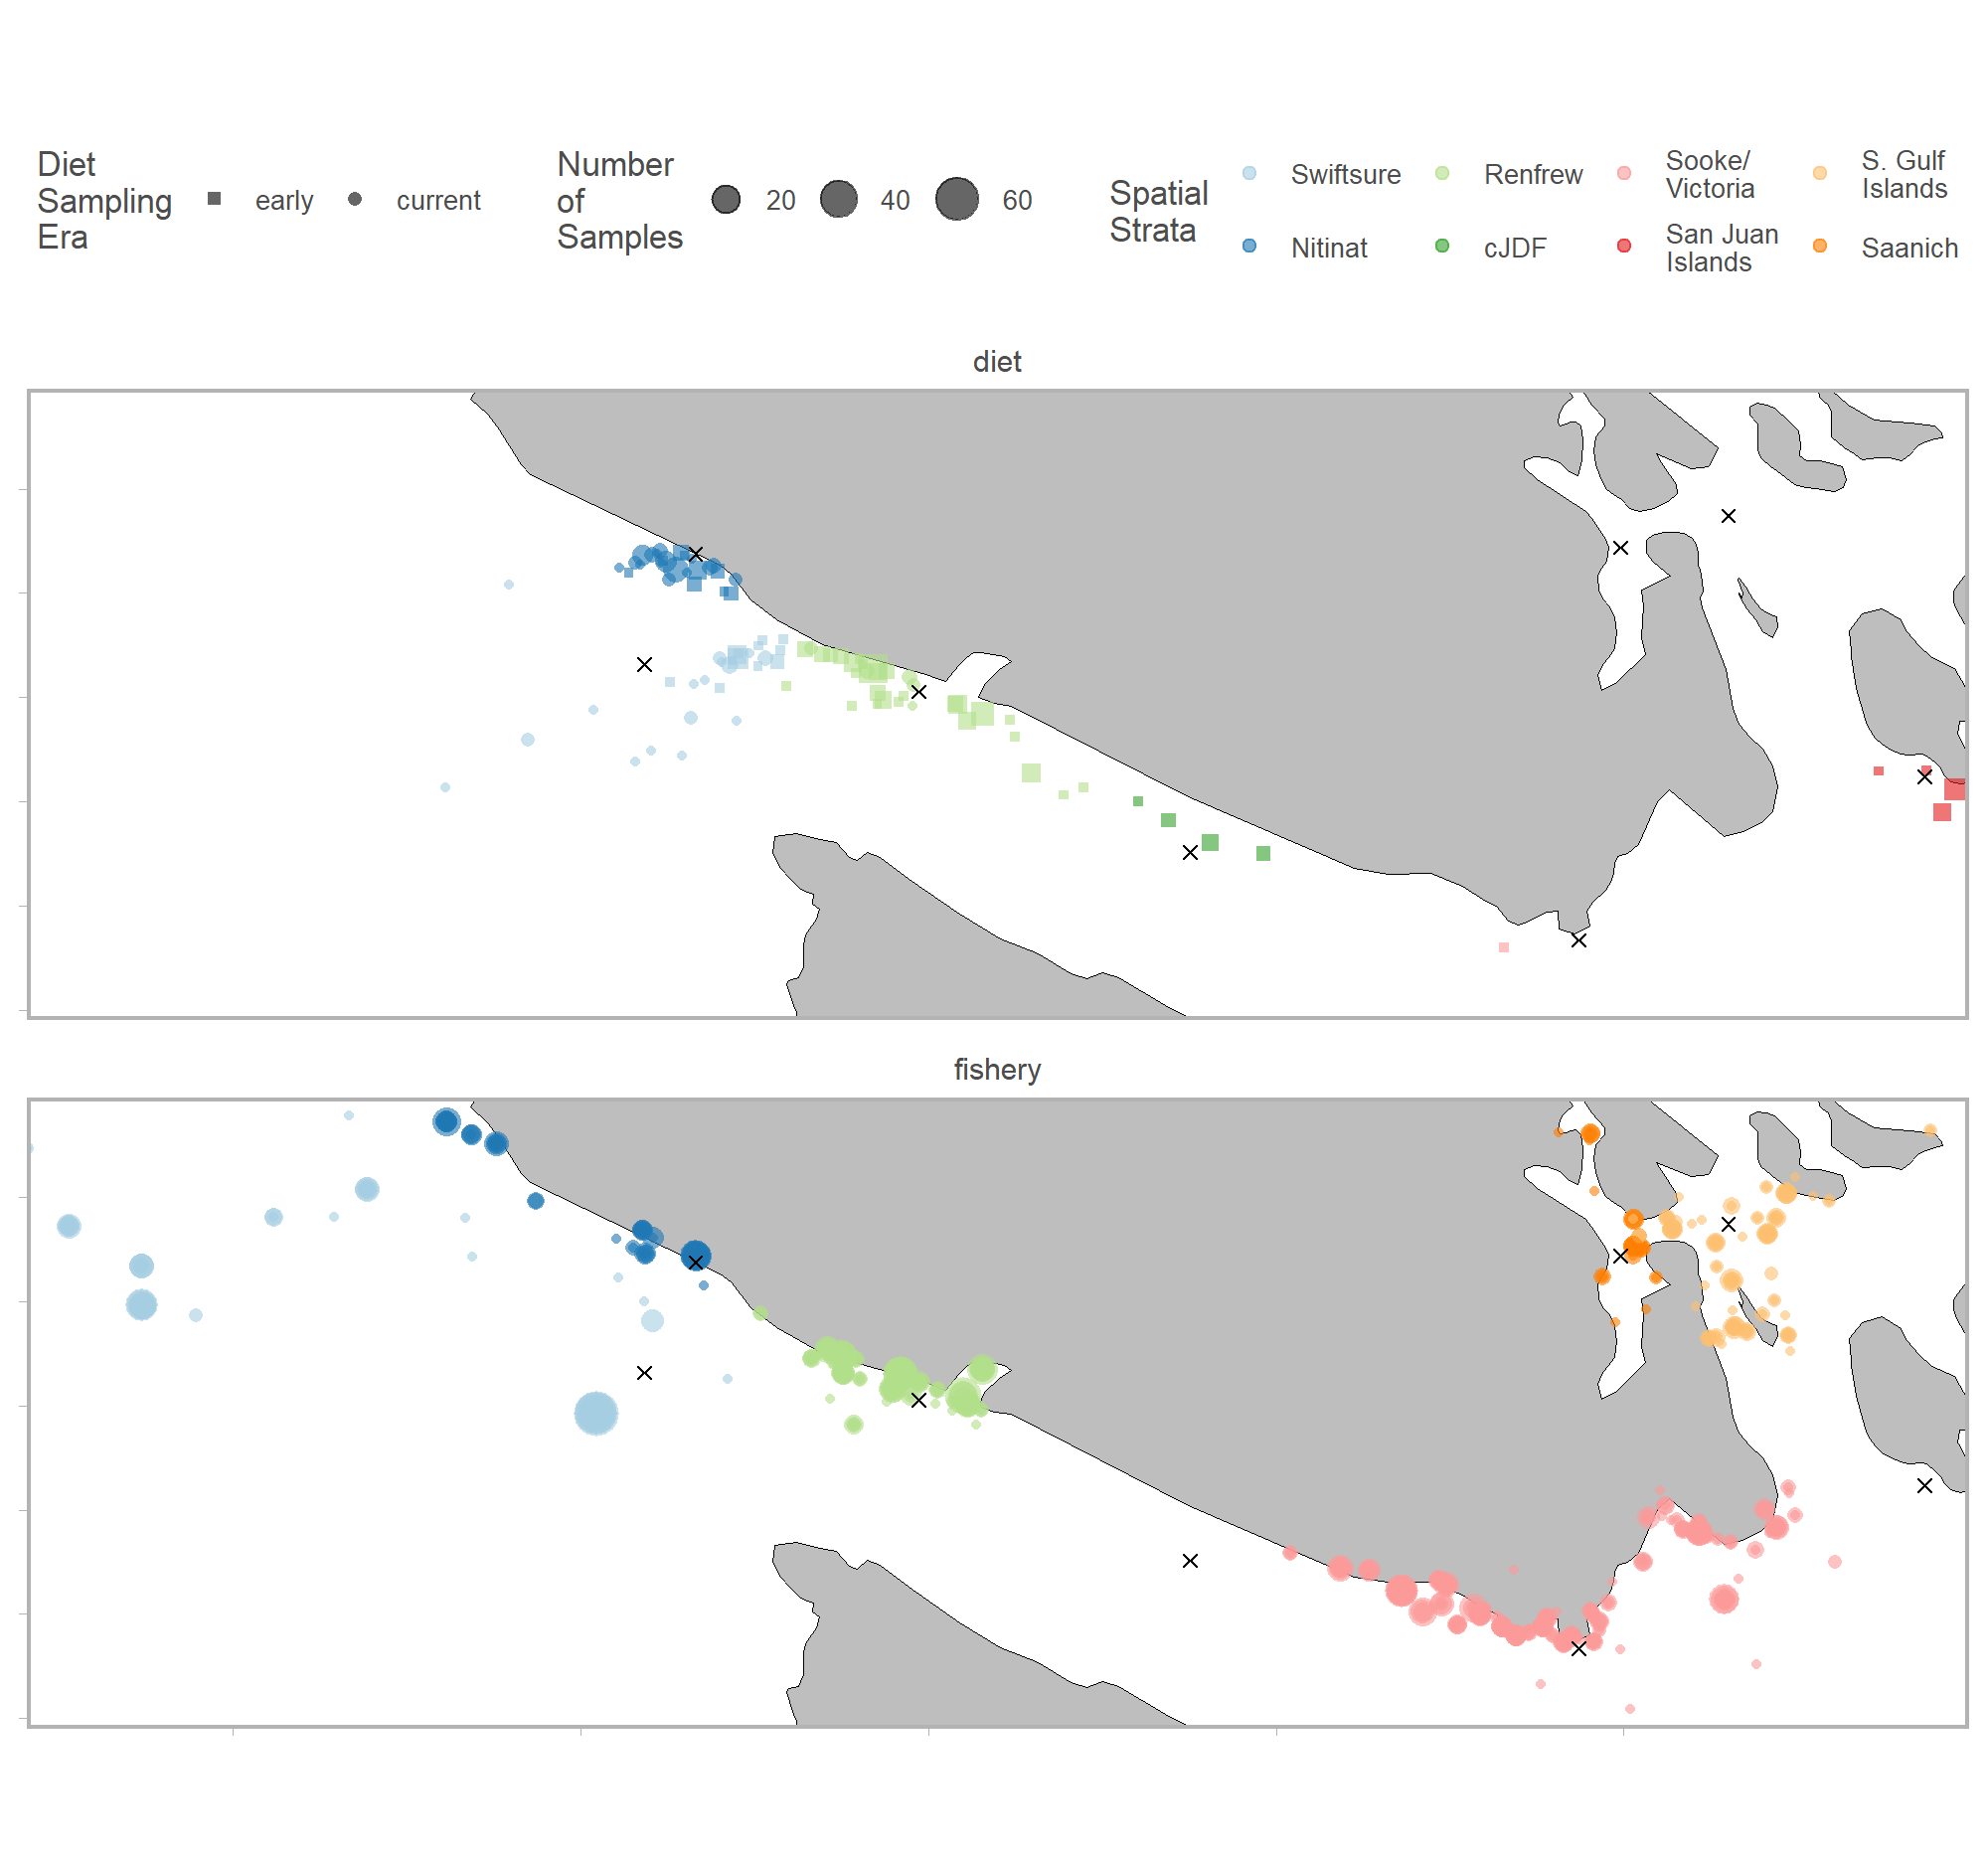
\includegraphics[width=5in]{figs/study_area.png}
    \caption{Zone d'étude dans le sud côtier de la Colombie-Britannique. La bathymétrie du fond marin représentée par l'ombrage bleu et l'habitat essentiel de l'ÉRES dénoté par le polygone ombragé gris.}
    \label{fig:study-area}
\end{figure}

\subsection{Échantillonnage des restes de proies de l'ÉRES}

La collecte des restes de proies d'épaulard résident a commencé en 1974 dans le cadre de l'étude à long terme du MPO sur l'histoire de vie des épaulards. De 2003 à 2013 (désignée comme « période d'échantillonnage précoce »), des relevés côtiers dédiés sur l'alimentation des ÉRE ont été entrepris principalement en utilisant un navire à moteur de 10 m \citep{fordChinookSalmonPredation2010, fordLinkingKillerWhale2010}. Les échantillons obtenus de 2017 à 2023 sont référés comme la « période d'échantillonnage actuelle » et ont été collectés principalement de relevés près du banc Swiftsure en utilisant des embarcations pneumatiques à coque rigide de 7 m \citep{thorntonSouthernResidentKiller2022}, avec trois années d'effort de relevé (2018-2020) s'étendant le long du détroit de Juan de Fuca jusqu'à Sooke (Figure \ref{fig:sampling-map}).

\begin{figure}[H]
    \centering
    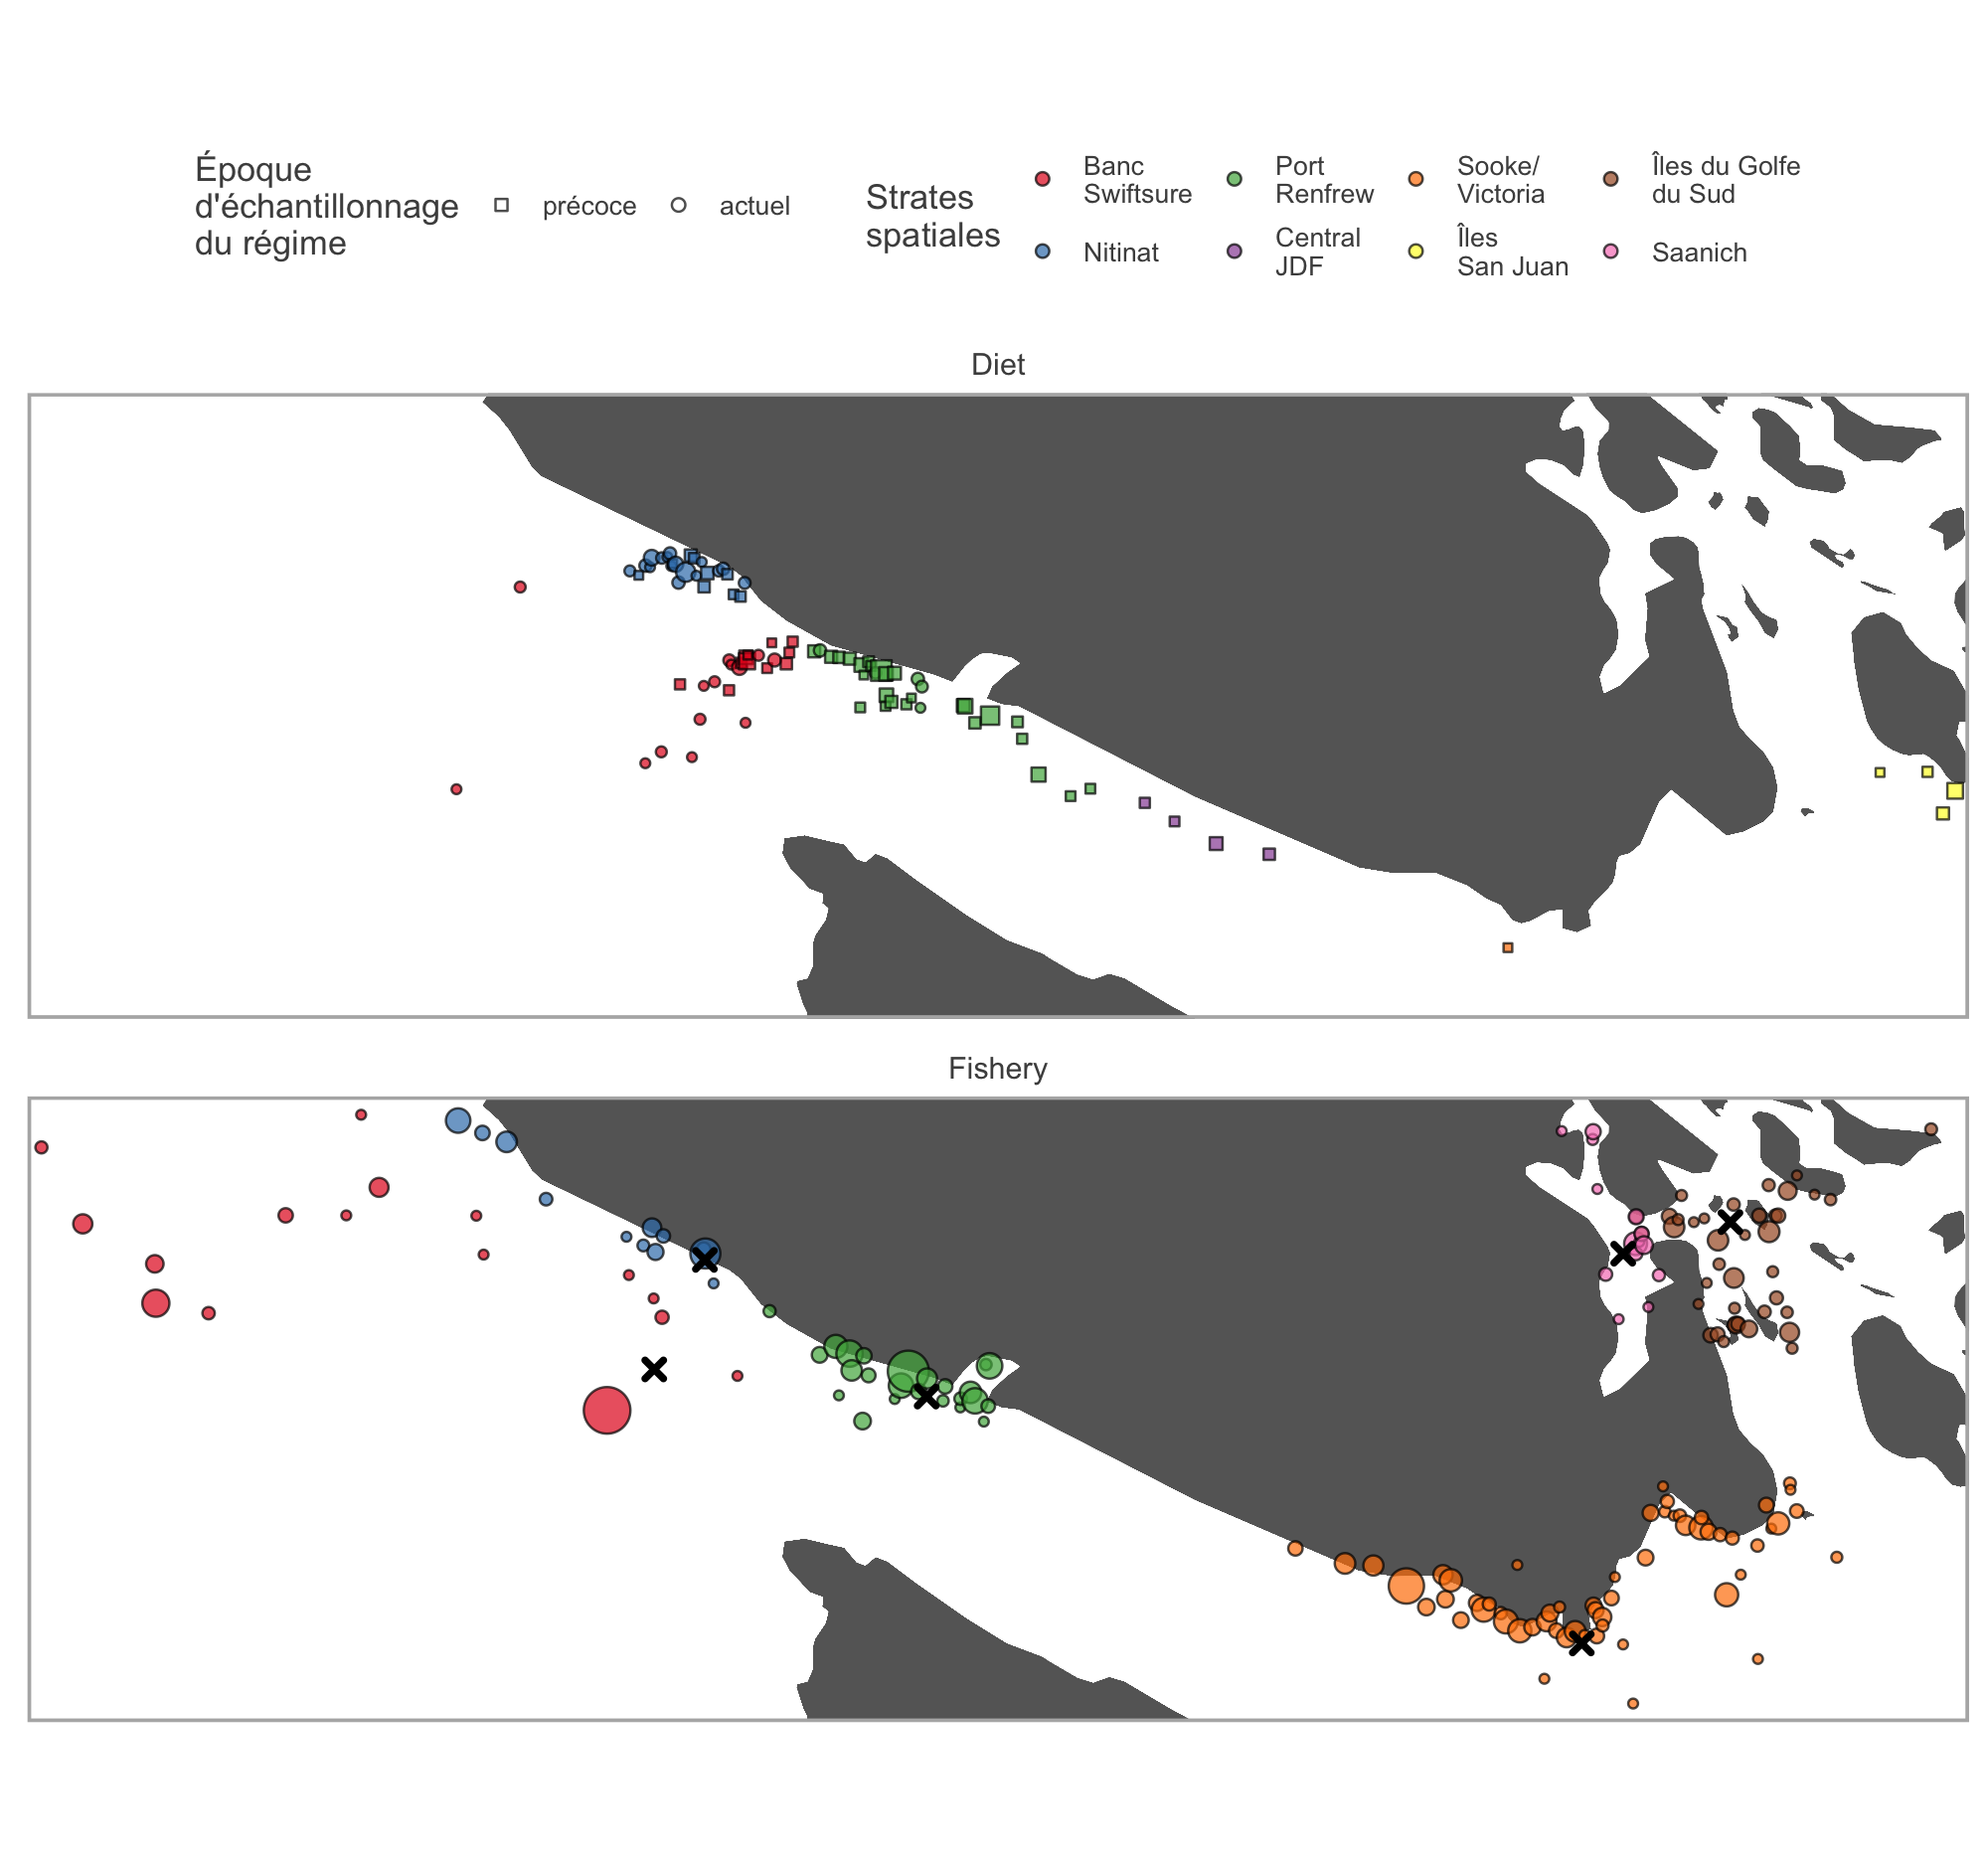
\includegraphics[width=5in]{figs/sampling_map.png}
    \caption{Emplacements des échantillons de composition des stocks de saumon chinook provenant des restes de proies de l'ÉRES (haut) et des pêcheries récréatives (bas). Les carrés et les cercles représentent les ères précoce (2003-2014) et actuelle (2017-2023), respectivement. Les points sont ombrés par strates spatiales et dimensionnés relativement au nombre d'échantillons collectés de cet emplacement sur toute la période d'étude. Les symboles 'x' noirs dans le panneau de pêcherie récréative sont des emplacements représentatifs dans chaque strate qui ont été utilisés pour générer des prédictions spatiales avec les modèles ajustés (Figures \ref{fig:stacked-rec}, \ref{fig:stacked-rec-size}). JDF central réfère au détroit de Juan de Fuca central.}
    \label{fig:sampling-map}
\end{figure}

Les protocoles de collecte d'échantillons utilisés dans les périodes d'échantillonnage précoce et actuelle étaient similaires. Quand des baleines étaient rencontrées, l'identification visuelle et photographique était initiée pour établir l'écotype, et si possible, déterminer le groupe, la matriligne, et/ou l'individu suivant les techniques d'identification décrites dans \cite{biggKillerWhalesStudy1987}. Le comportement des baleines était observé pour tout signe de comportement d'alimentation ou de fourrage actif (événements de prédation ; voir \citet{stredulinskyDelineatingImportantKiller2023} pour une description des indices comportementaux). Quand un événement de prédation est suspecté, le navire était déplacé à travers l'empreinte de nageoire caudale de la baleine pour chercher des écailles et tissus flottants. Les échantillons biologiques (p. ex., écailles, tissus de proie) étaient collectés en utilisant un filet à épuisette et retirés du filet en utilisant des pinces stériles et placés dans des fioles de scintillation en verre de 20 mL contenant 10 mL d'éthanol à 95\% pour identification subséquente. Les trois groupes d'ÉRES utilisent la partie ouest de l'habitat essentiel canadien pendant l'été et des restes de proies ont été collectés de chaque groupe, bien que trop peu étaient disponibles pour tester les différences spécifiques aux groupes.

Il est possible que les restes de proies échantillonnés puissent ne pas être représentatifs des régimes alimentaires de l'ÉRES. Premièrement, la diversité d'espèces dans les régimes alimentaires de l'ÉRES estimée à partir d'échantillons fécaux (présumés être non biaisés) est typiquement plus élevée que celle des échantillons de débris de proies \citep{hansonEndangeredPredatorsEndangered2021}, probablement due aux différences spécifiques aux espèces dans la probabilité que les débris soient collectés. Ces effets ne sont pas pertinents ici, cependant, parce que nous nous sommes concentrés seulement sur le saumon chinook. Deuxièmement, les restes de proies peuvent refléter les proies consommées près de la surface, qui peuvent être plus susceptibles d'être des proies orientées vers la surface ou de grande taille. Pourtant, les données de marquage suggèrent que les épaulards résidents identifient les proies de saumon du Pacifique à des profondeurs modérées, poursuivent des proies individuelles en eau profonde, et consomment ensuite les proies près de la surface \citep{wrightBehavioralContextEcholocation2021}. Ces comportements sont consistants à travers une gamme relativement large d'espèces et de classes de taille de saumon du Pacifique \citep{wrightBehavioralContextEcholocation2021}. Troisièmement, les événements d'échantillonnage de l'ÉRES peuvent ne pas être indépendants. Sans modèle statistique, nous ne pouvons pas quantifier l'autocorrélation spatiale ou temporelle dans les restes de proies ; cependant, les échantillons collectés le même jour et en proximité proche provenaient souvent de multiples stocks, suggérant une autocorrélation modeste (Figures \ref{fig:prey-samples-2007}, \ref{fig:prey-samples-2017}).

\begin{figure}[H]
    \pdftooltip{\centering
    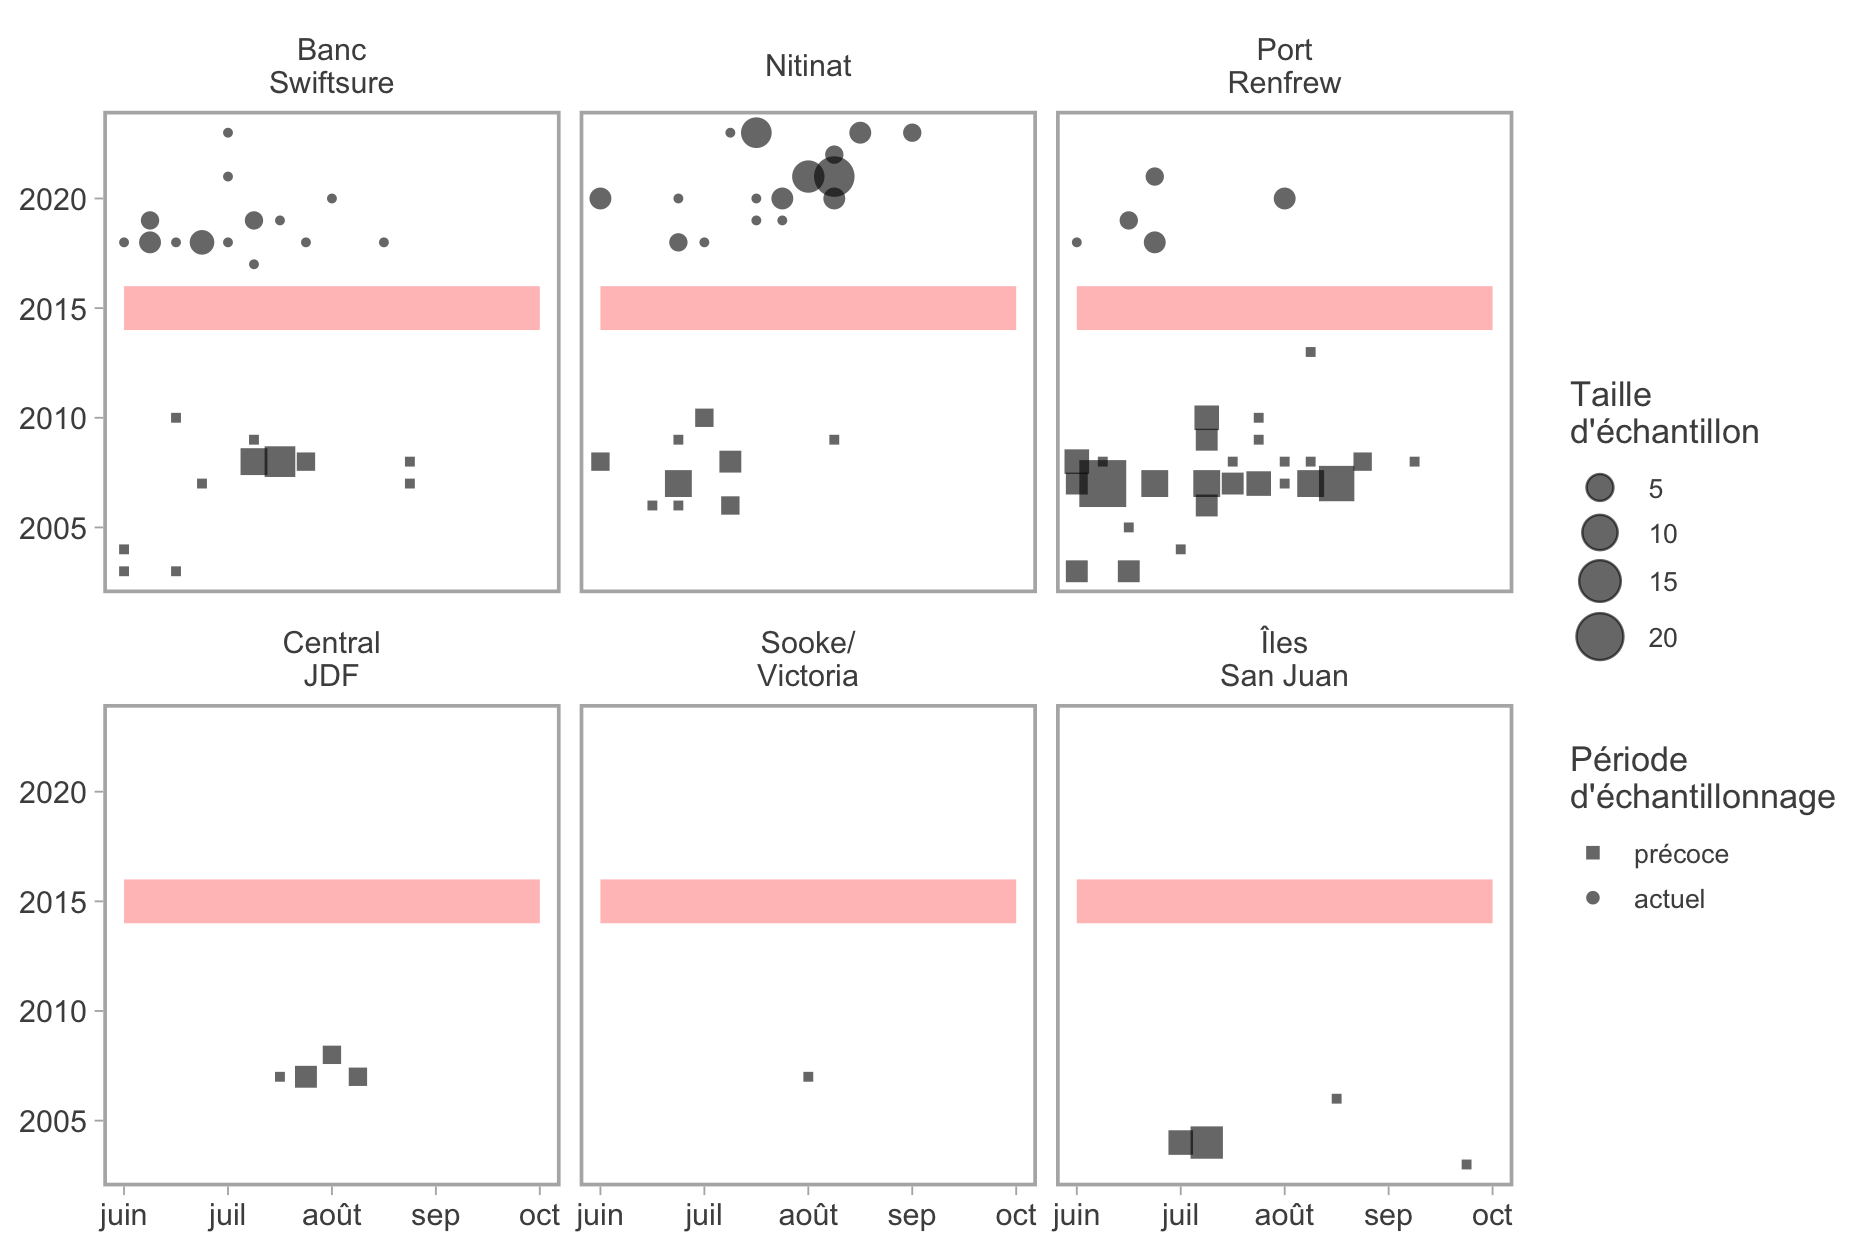
\includegraphics[width=5in]{figs/temporal_sample_coverage.png}}{Figure \ref{fig:temporal-diet-samples}}
    \caption{Distribution temporelle des échantillons de composition des stocks de saumon chinook des restes de proies de l'ÉRES. Les strates (panneaux) correspondent aux domaines spatiaux dans la Figure \ref{fig:sampling-map}. Les périodes d'échantillonnage précoce et actuelle sont représentées par des carrés et des cercles, respectivement, avec le polygone rouge montrant les années intermédiaires. La taille des points mise à l'échelle du nombre d'échantillons collectés dans une semaine et année données.}
    \label{fig:temporal-diet-samples}
\end{figure}

\subsection{Échantillonnage des pêcheries récréatives de saumon chinook}

La section d'évaluation des stocks de la côte sud du MPO collecte des données biologiques des pêcheries récréatives en eau salée à travers le sud de la Colombie-Britannique. Depuis 2014, ces données ont inclus des échantillons d'écailles et de tissus, des mesures de longueur à la fourche, de l'information sur si la nageoire adipeuse d'un poisson est intacte ou coupée, et, quand présentes, des marques à fil codé (MFC) qui assignent un individu à un groupe de lâcher d'écloserie spécifique. Des détails additionnels sur comment les échantillons biologiques sont utilisés pour déterminer l'âge et l'identité de stock sont fournis ci-dessous.

Les échantillons de pêcherie ont été collectés de trois programmes de terrain. La majorité provenait du programme d'observateur d'enquête au quai, où les échantillons sont collectés pendant des entrevues avec des pêcheurs récréatifs. Le programme d'observateur au quai échantillonne seulement les prises débarquées (c.-à-d., poissons retenus pour la récolte). Une portion d'échantillons a été collectée par un programme de science citoyenne, les Avid Anglers, qui est une collaboration entre le MPO, le British Columbia Sport Fishing Institute, les récolteurs récréatifs, et les guides de pêche sportive. Les participants fournissent des données sur la taille et le statut de coupe adipeuse pour tout le saumon qu'ils rencontrent (gardé et relâché), ainsi que des échantillons pour l'identification génétique de stock (IGS). Les échantillons proviennent principalement des prises débarquées ; cependant, les Avid Anglers collectent aussi des échantillons génétiques des poissons relâchés des pêcheries de non-rétention (bien que la fréquence d'échantillonnage dans les pêcheries de non-rétention varie spatialement). Finalement, les échantillons de 2022 et 2023 incluent des données collectées par le personnel scientifique du MPO pendant les Pêcheries de référence, un programme de recherche en collaboration avec le Sport Fishing Institute pour collecter des données biologiques pour évaluer les impacts des pêcheries sélectives de marque. Les Pêcheries de référence échantillonnent tout le saumon chinook rencontré et sont donc représentatives des prises débarquées et relâchées. Nous n'avons pas stratifié basé sur le programme de terrain parce que les échantillons Avid Angler des prises débarquées ne pouvaient pas être distingués de façon fiable de l'échantillonnage au quai des prises débarquées.

Les données dépendantes de la pêcherie peuvent être biaisées dues à des facteurs tels que la sélectivité de l'engin ou le comportement du pêcheur. Ces effets sont amplifiés par les interventions de gestion telles que les pêcheries sélectives de marque ou les limites de taille. Les pêcheries récréatives dans la zone d'étude ont été impactées par des interventions de gestion qui varient saisonnièrement, spatialement, et parmi les années (Figure \ref{fig:temporal-fishery-samples-management} ; voir Dobson et al. 2020 et MPO 2023 pour détails). Bien que notre ensemble de données inclut des échantillons d'individus relâchés, qui sont présumément moins biaisés que les prises débarquées, ceux-ci constituaient une proportion relativement petite du total (approximativement 5\%). Une analyse préliminaire a indiqué que les estimations de composition des stocks étaient similaires indépendamment de si les échantillons de poissons relâchés étaient ou n'étaient pas inclus (résultats non montrés), et toutes les analyses subséquentes ont inclus les échantillons relâchés. Malheureusement, une évaluation plus robuste des effets de sélectivité n'était pas possible due au calendrier et à l'emplacement déséquilibrés des mesures de gestion ; cependant, nous décrivons qualitativement les impacts potentiels des mesures de gestion à nos conclusions dans la discussion.

Les échantillons biologiques incluaient un code d'emplacement représentant l'emplacement de pêche (soit rapporté à l'observateur d'enquête ou enregistré par l'Avid Angler ou le personnel scientifique). Les codes d'emplacement étaient géoréférencés pour fournir une latitude et longitude pour chaque échantillon. En d'autres mots, chaque échantillon de pêcherie avait un emplacement approximatif représentant un site de pêche communément utilisé, pas un emplacement précis basé sur où le poisson a été capturé (Figure \ref{fig:sampling-map}). Bien que la couverture variait spatialement, l'échantillonnage a eu lieu dans certaines régions dans tous les mois (Figure \ref{fig:temporal-fishery-samples}).

\begin{figure}[H]
    \centering
    \pdftooltip{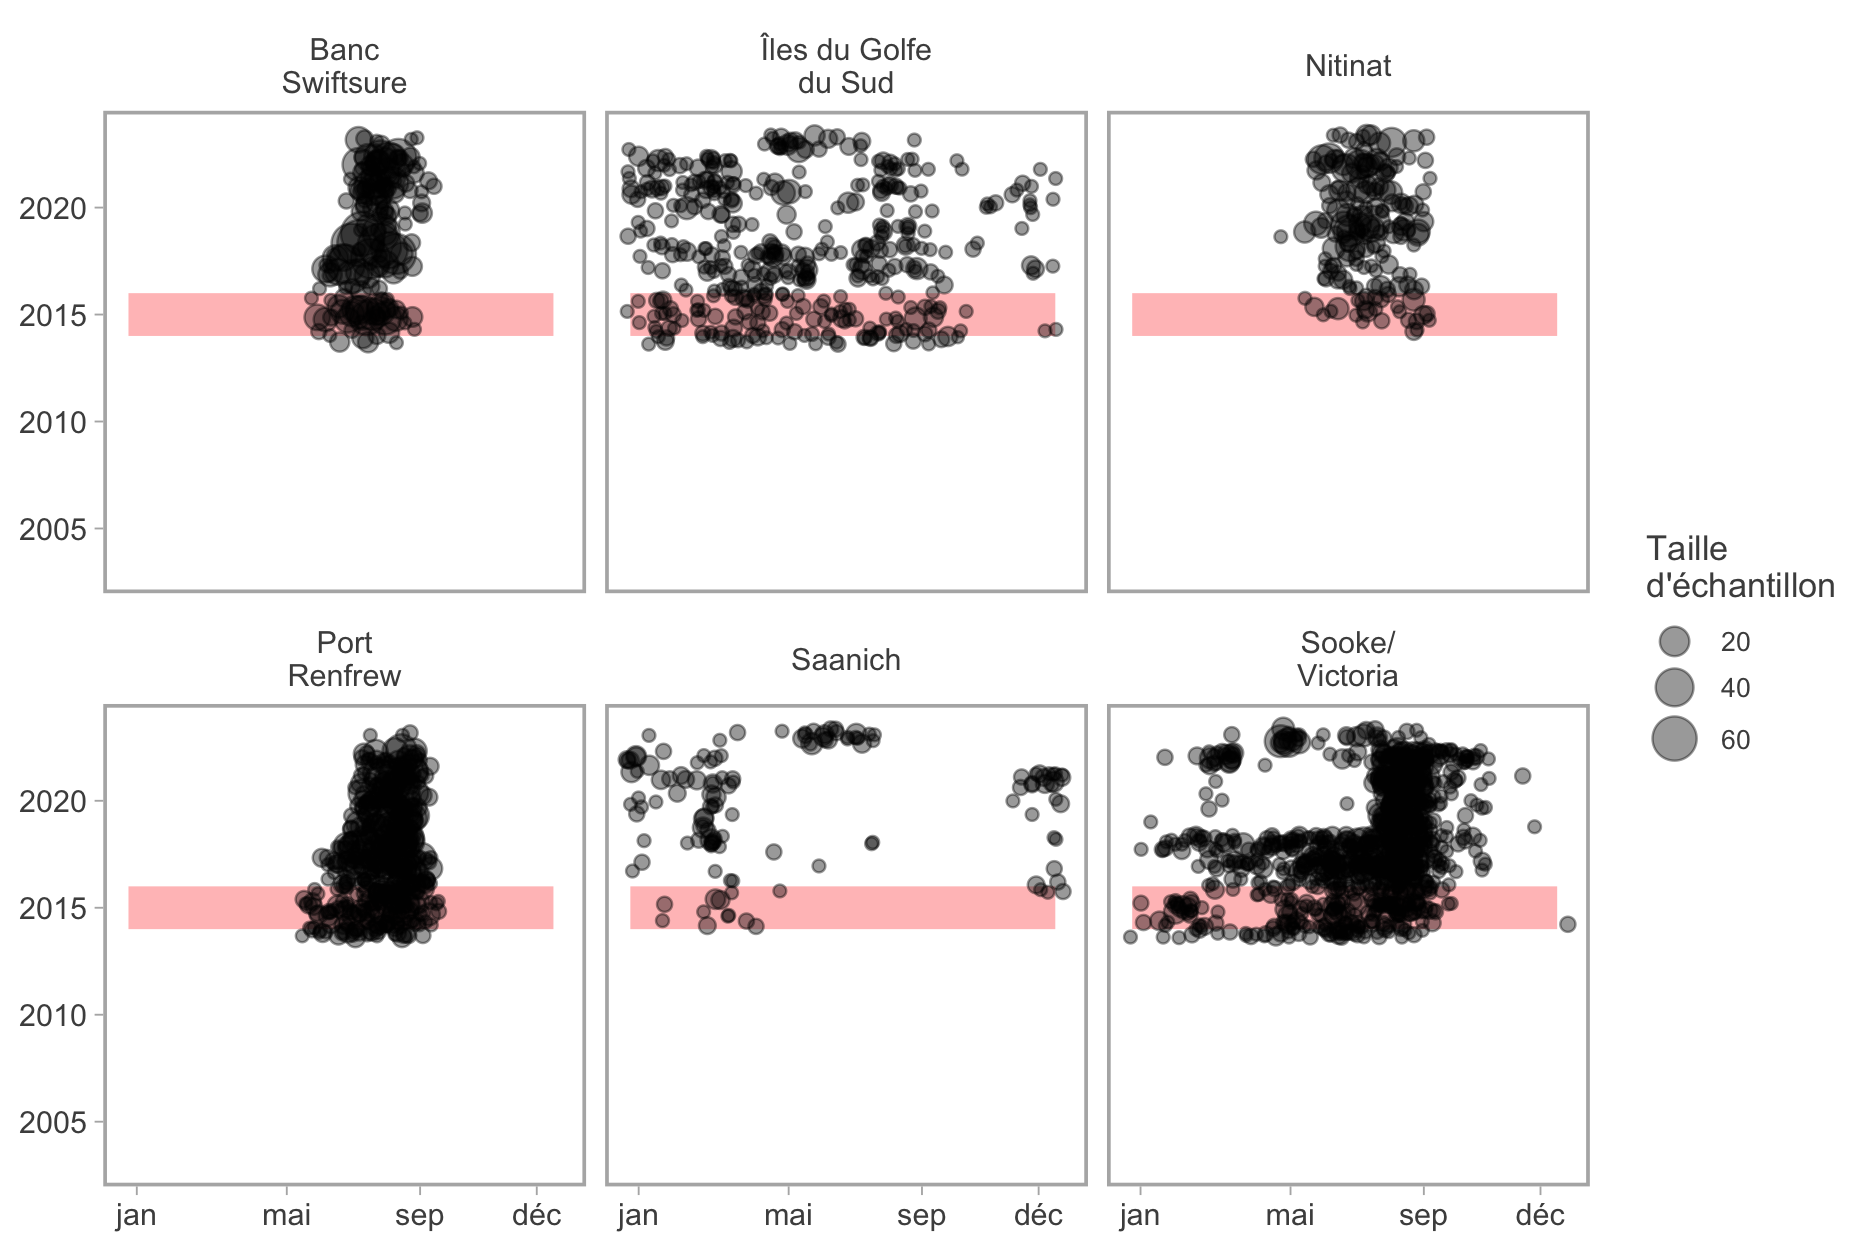
\includegraphics[width=5in]{figs/rec_temporal_sample_coverage.png}}{Figure \ref{fig:temporal-fishery-samples}}
    \caption{Distribution temporelle des échantillons de composition des stocks de saumon chinook des pêcheries récréatives. Les strates (panneaux) correspondent aux domaines spatiaux dans la Figure \ref{fig:sampling-map}. Les années intermédiaires sans échantillons de proies sont représentées par un polygone rouge montrant qu'aucun échantillon de pêcherie n'est disponible de la période d'échantillonnage précoce des restes de proies de l'ÉRES (Figure \ref{fig:temporal-diet-samples}). La taille des points mise à l'échelle du nombre d'échantillons individuels collectés dans un emplacement de pêche, une semaine, et une année donnés. Les points ont été décalés pour maximiser la visibilité. Notez que les échantillons de pêcherie, contrairement aux échantillons de restes de proies, ont été collectés tout au long de l'année.}
    \label{fig:temporal-fishery-samples}
\end{figure>

L'avantage principal de cet ensemble de données relativement aux données de récupération de MFC plus communément utilisées est la précision avec laquelle les échantillons peuvent être assignés à un emplacement et une période de temps. Le programme MFC vise à estimer les taux d'exploitation spécifiques aux stocks à travers une échelle spatiale large — un objectif similaire, mais distinct, à l'estimation des estimations spatialement et temporellement explicites de composition des stocks. Parce que les estimations dérivées de MFC des taux d'exploitation requièrent un nombre relativement grand de récupérations de marques par pêcherie pour être suffisamment précises, elles sont communément agrégées à des échelles saisonnières (p. ex., multiples mois) et régionales (p. ex., sud-ouest de l'île de Vancouver vs. sud du détroit de Georgie). De plus, plusieurs stocks canadiens, incluant Fraser River Spring $5_2$ et Summer $5_2$, qui peuvent être des proies clés des ÉRES ne sont pas adéquatement représentés par les indicateurs MFC actuels.

\subsection{Assignation des échantillons aux stocks, classes de taille, et écloseries}

\subsubsection{Échantillons de proies de l'ÉRES}

Les écailles collectées après un événement de prédation de l'ÉRES ont été montées et examinées visuellement en utilisant des projecteurs Leitz Neopromar pour évaluer les patrons d'anneaux marins et d'eau douce. L'espèce et l'âge ont été déterminés des lectures d'écailles par des âgeurs expérimentés au Laboratoire de vieillissement des poissons au Laboratoire de sclérochronologie de la Station biologique du Pacifique (Pêches et Océans Canada, Nanaimo, Colombie-Britannique, Canada). Le laboratoire fournit une estimation du nombre d'années qu'un saumon a passé dans les habitats d'eau douce et océanique (c.-à-d., âge d'eau douce et marin respectivement) basée sur les incréments de croissance annuels. Puisque la majorité de la croissance du saumon chinook se produit pendant la résidence océanique et les âges d'eau douce n'étaient pas toujours disponibles pour les échantillons de pêcherie, nous avons concentré les analyses sur l'âge marin. De plus, nous avons incorporé l'erreur de vieillissement dans les estimations des restes de proies de l'ÉRES et utilisé l'âge marin, incluant cette erreur, pour prédire la longueur à la fourche des proies de l'ÉRES basée sur les relations taille-selon-l'âge spécifiques aux stocks (détails dans l'Appendice \ref{size-at-age}).

Les échantillons d'écailles et les restes de tissus post-prédation ont été soumis au Laboratoire de génétique moléculaire du MPO à la Station biologique du Pacifique pour l'identification d'espèce et de stock. L'identification des stocks de saumon chinook a suivi la méthodologie décrite dans Beacham et al. (2018)\nocite{beachamParentagebasedTaggingGenetic2022}. Brièvement, l'ADN a été extrait et l'amplification PCR de 321 amplicons cibles a été conduite en utilisant un pool d'amorces développé à partir de données de séquence de saumon chinook publiées. Les échantillons ont ensuite été identifiés au stock en utilisant soit a) une méthodologie de séquençage d'amplicon SNP ciblée ou b) des marques basées sur la parenté (PBT). Sous le programme PBT, les géniteurs d'écloserie sont génotypés, permettant aux descendants échantillonnés d'être assignés aux individus parents et identifiés comme d'origine d'écloserie (détails ci-dessous), avec un haut degré de confiance \citep{beachamParentagebasedTaggingGenetic2022}. Nous avons agrégé les assignations de stocks individuels pour améliorer l'interprétabilité (détails additionnels ci-dessous).

\subsubsection{Échantillons de pêcherie récréative}

L'identité de stock pour les échantillons collectés de la pêcherie récréative a été inférée en faisant correspondre les MFC ou otolithes récupérés aux cohortes de lâcher ou en utilisant des échantillons de tissus avec des SNP ou des microsatellites \citep{beachamPacificRimPopulation2006a, beachamParentagebasedTaggingGenetic2022}. Étant donné le grand nombre de stocks de saumon chinook présents dans le sud de la Colombie-Britannique, nous avons agrégé les assignations individuelles, qui ont été faites approximativement à l'échelle des populations de frai, pour rendre les analyses subséquentes traitables.

Au Canada, le saumon chinook est évalué au niveau de l'UC \citep{holtbyConservationUnitsPacific2007} ; cependant, les actions de gestion domestiques se concentrent souvent sur les unités de gestion de stock (UGS) qui contiennent une ou plusieurs UC. Bien que les UC dans une UGS peuvent ne pas frayer en proximité proche, une seule UGS a typiquement une distribution marine et une phénologie de migration relativement homogènes. Les UC par définition excluent les poissons d'origine d'écloserie, tandis que les UGS ne le font pas. Puisque notre analyse était concentrée sur le contexte de gestion canadien, nous avons agrégé la plupart des populations canadiennes au niveau UGS (Figure \ref{fig:stock-map}, Tableau S1). Nous avons de plus agrégé les UGS Lower Georgia Strait, Middle Georgia Strait, Upper Georgia Strait, et Southern Mainland Inlet comme East Coast Vancouver Island et Southern Mainland Inlets (ECVI/SOMN) puisque ces UGS étaient relativement rarement rencontrées (Figure \ref{fig:stock-map}, Tableau S1). Nous avons assigné les individus restants à un de quatre groupements régionaux : Puget Sound, Columbia River et Snake River spring-run, Columbia et Snake river summer/fall-run (incluant les poissons Willamette River spring-run due à une distribution marine similaire), et un agrégat (« Autre ») incluant les populations rares du nord de la Colombie-Britannique, de la côte de Washington et Oregon, et de Californie (Figure \ref{fig:stock-map}, Tableau S1). Nous soulignons que les stocks Columbia River et « Autre » regroupent des populations avec des histoires de vie disparates, mais étant donné le focus de gestion canadien de cette analyse et la nécessité d'ajuster un modèle traitable, nos groupements permettent qu'une inférence raisonnable soit tirée. À travers ce manuscrit, nous utilisons les termes « stock » et « composition des stocks » quand nous référons à ces groupements spécifiques, ainsi qu'aux agrégats génériques de populations de saumon chinook.

\begin{figure}[H]
    \centering
    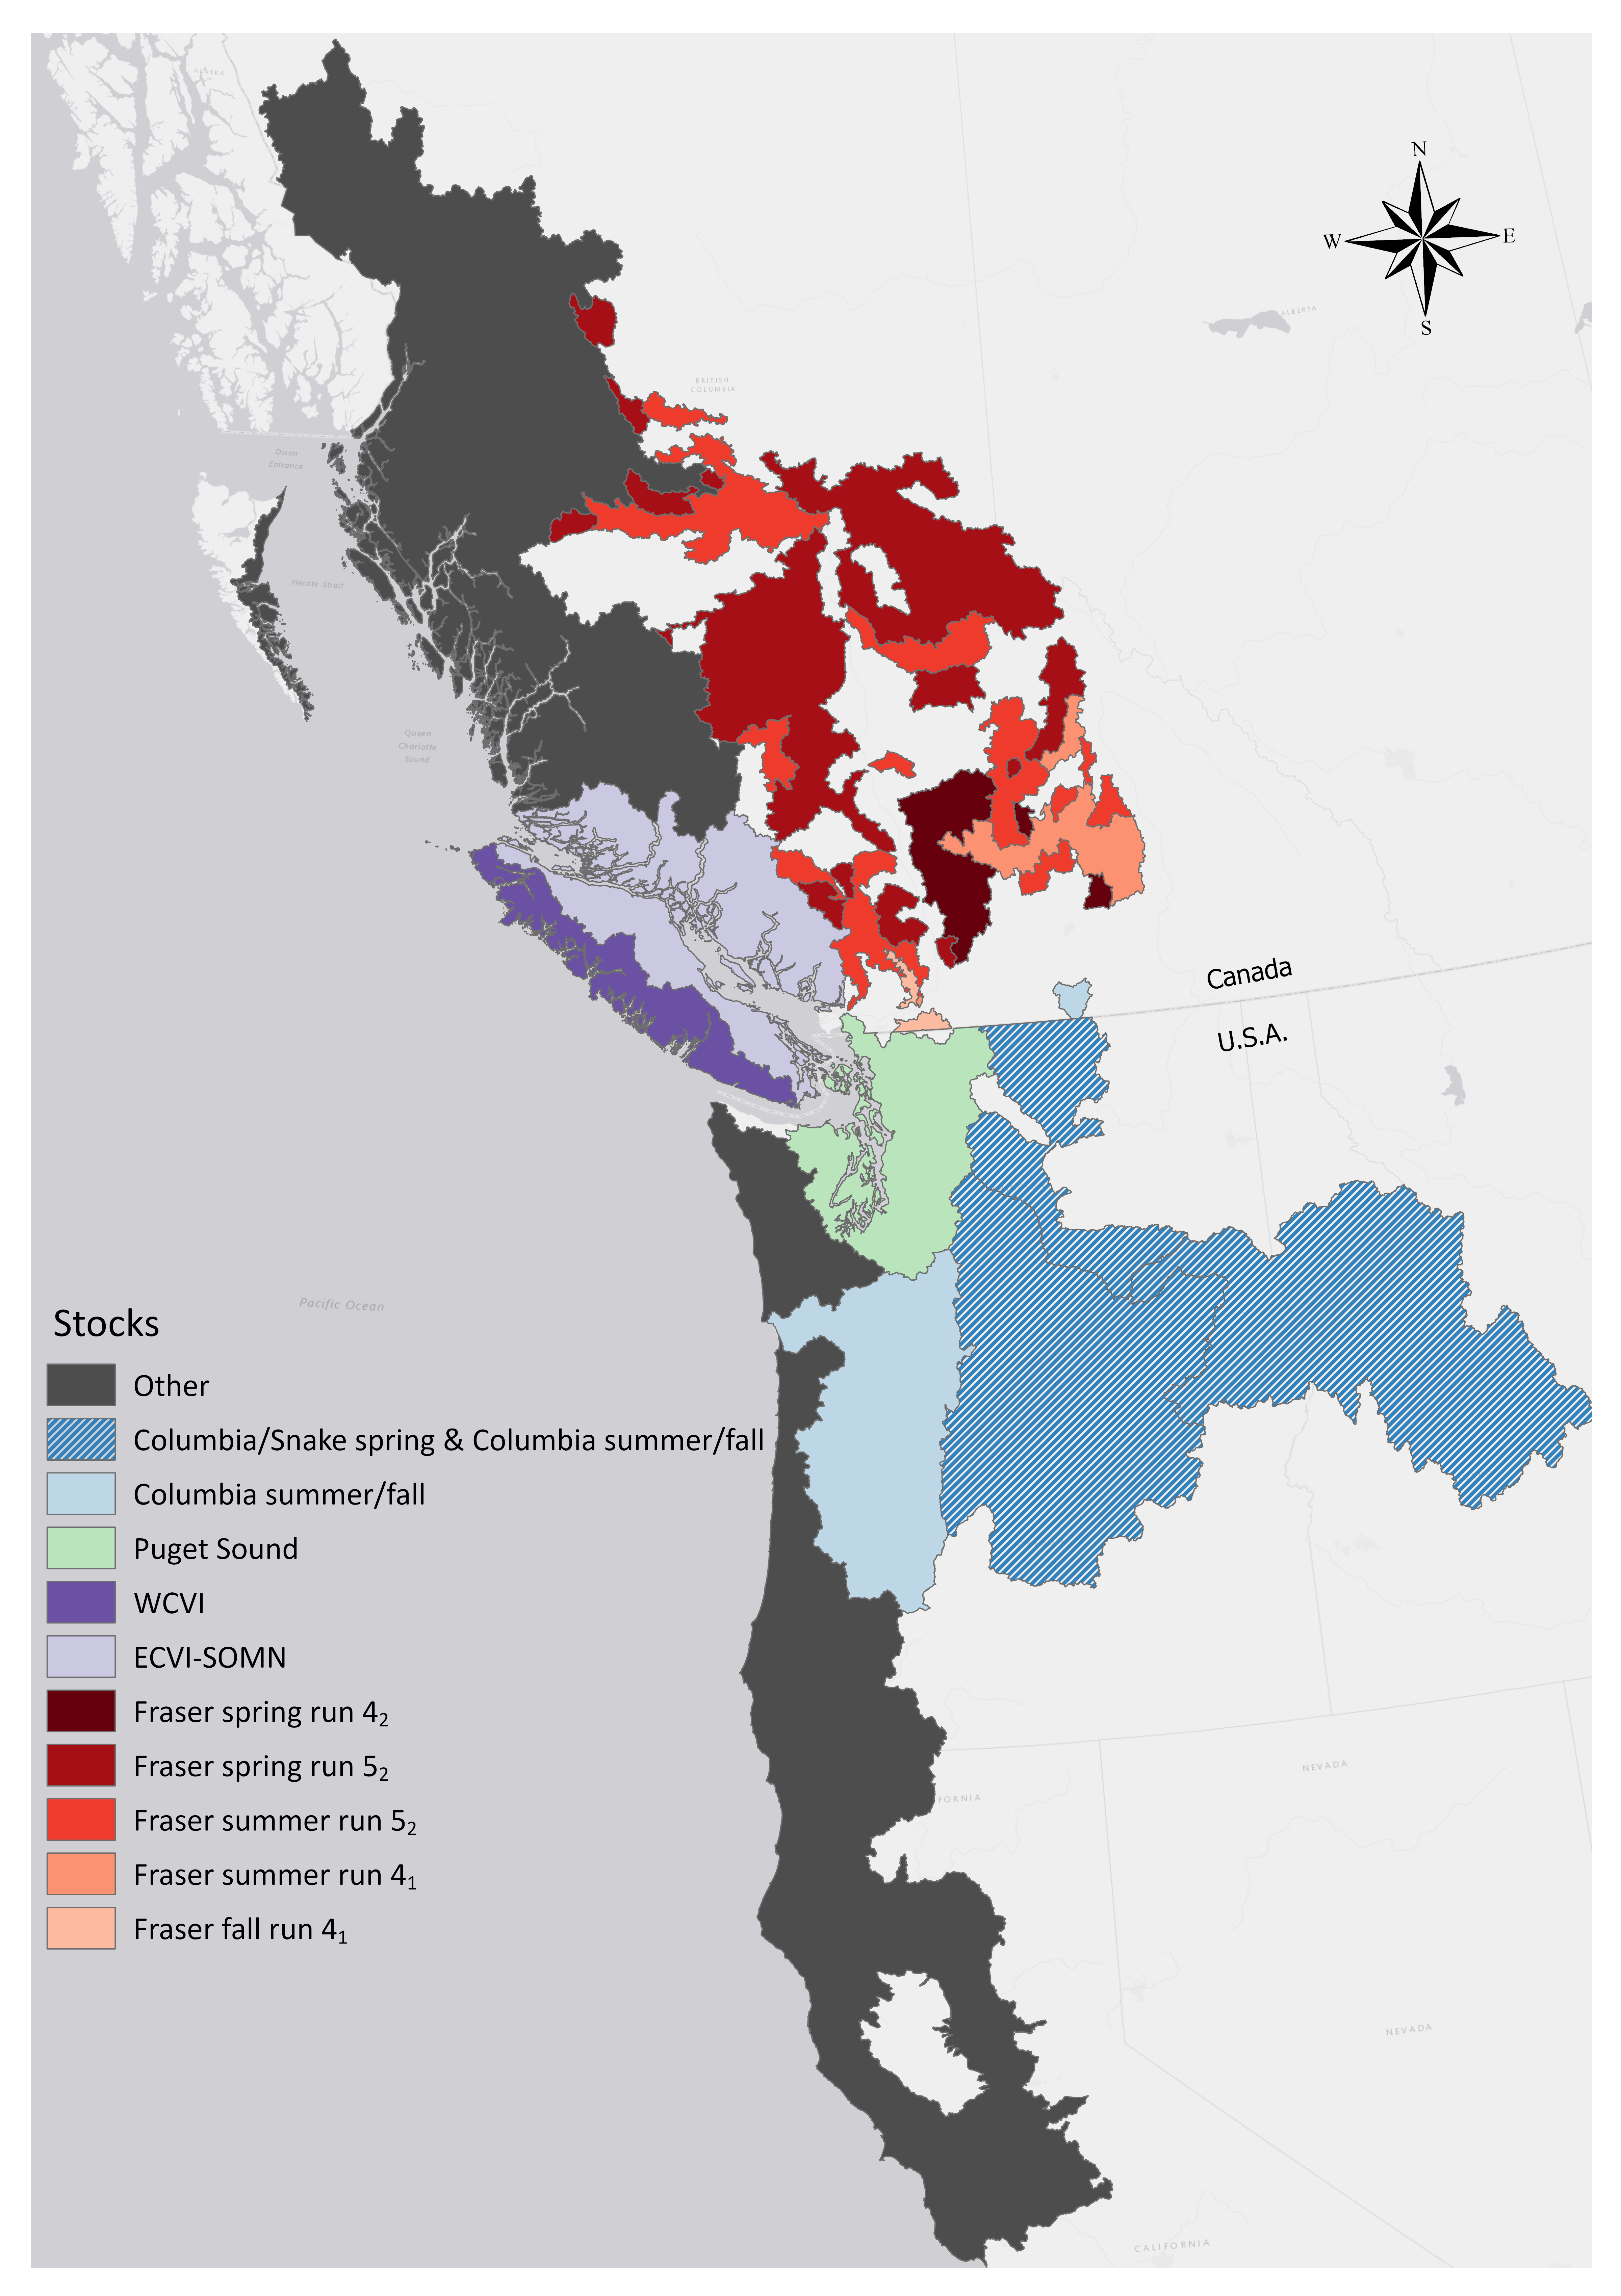
\includegraphics[width=5in]{figs/chinook_stock_map.png}
    \caption{Bassins versants contenant les cours d'eau natals pour chaque stock de saumon chinook. Notez que tous les bassins versants avec des populations Columbia River Spring contenaient aussi des populations Columbia River Summer/Fall et sont représentés par des hachures.}
    \label{fig:stock-map}
\end{figure}

Pour modéliser la variabilité dans la taille du saumon chinook, nous avons créé quatre casiers de taille basés sur la longueur à la fourche à la capture : moins de 65 cm, 65-75 cm, 75-85 cm, et plus de 85 cm. Les poissons plus petits que les limites de taille minimales (soit 62 ou 45 cm de longueur à la fourche selon la zone de gestion) peuvent être échantillonnés et relâchés ; cependant, nous avons inclus seulement les poissons plus grands que 55 cm dans les analyses subséquentes. Les données d'âge pour un sous-ensemble d'individus (n = 7815) étaient disponibles des MFC, PBT, ou estimées en utilisant les anneaux d'écailles (détails ci-dessus).

Nous avons utilisé de multiples approches pour identifier la contribution relative des poissons d'origine d'écloserie dans les échantillons des pêcheries récréatives. Les poissons avec des nageoires adipeuses manquantes ont été identifiés comme d'origine d'écloserie. Les taux de marquage (la proportion de lâchers d'écloserie où les nageoires adipeuses sont retirées) sont presque 100\% dans les écloseries de Washington et Oregon \citep{andersonReviewHatcheryReform2020, wdfwAnadromousSalmonSteelhead2021, odfwFishPropagationAnnual2022}, mais les écloseries de Colombie-Britannique marquent seulement une proportion relativement petite d'individus \citep{pscLessonsLearnedReport2016}. Par conséquent, nous avons aussi utilisé les marques thermiques d'otolithes et l'échantillonnage génétique pour identifier les individus d'origine d'écloserie.

Les écloseries de Colombie-Britannique ont commencé à implémenter le PBT dans l'année de géniteur 2013 et bien que la couverture dans les grandes installations d'amélioration soit typiquement élevée, elle a varié dans le temps (Figure \ref{fig:pbt-coverage}). Les individus avec une assignation PBT ont été identifiés comme d'origine d'écloserie, tandis que ceux identifiés comme provenant de stocks qui ne sont pas présents dans la ligne de base PBT ont été identifiés comme sauvages. Finalement, les individus avec des nageoires adipeuses intactes et des assignations GSI à des stocks avec de faibles taux de marquage et aucune donnée PBT (p. ex., Californie, Alaska) ou appartenant à des années de géniteur dans lesquelles l'écloserie pertinente de Colombie-Britannique avait un taux PBT relativement faible (ici défini comme moins de 80\% de couverture de géniteurs (Figure \ref{fig:pbt-coverage})) ont été assignés une classification « inconnue ». Étant donné que de nombreux échantillons de pêcherie récréative ne pouvaient pas être assignés de façon définitive un statut d'écloserie ou sauvage, et que les contributions d'écloserie covarient avec l'identité de stock, nous n'avons pas ajusté un modèle statistique aux données assignées d'écloserie.

Contrairement aux analyses précédentes \cite[p. ex.,][]{freshwaterIntegratedModelSeasonal2021}, nous n'avons pas mis à l'échelle les estimations de composition des stocks par les prises de saumon chinook par unité d'effort pour dériver un indice d'abondance spécifique aux stocks parce que la comparaison principale d'intérêt était entre la composition de la pêcherie et la composition des restes de proies. De plus, les estimations de prises et d'effort sont typiquement les plus fiables aux échelles de sous-zone d'enquête et mensuelles (ou plus grossières), ce qui diluerait la résolution spatio-temporelle des estimations de composition des stocks. Finalement, nous assumons déjà que la pêcherie récréative échantillonne la composition du saumon chinook d'une manière analogue aux ÉRES (exploré en détail dans la Discussion). Les estimations d'abondance spécifiques aux stocks incorporent des assumptions de sélectivité additionnelles qui peuvent ne pas être valides.

\subsection{Proportion de géniteurs d'origine d'écloserie}

Pour mieux comprendre la variation parmi les stocks canadiens dans l'amélioration d'écloserie, nous présentons à la fois des estimations basées sur l'individu des contributions d'écloserie (décrites dans la section précédente) et des estimations de la proportion de géniteurs d'origine d'écloserie (pHOS). Les estimations de pHOS ont été fournies par le Programme d'amélioration des salmonidés de Pêches et Océans Canada et étaient disponibles pour les années de retour entre 2014 et 2022, bien que le nombre d'années disponibles variait parmi les populations de frai. Puisque chaque stock contient de multiples populations de frai, nous avons calculé le pHOS moyen, par stock, en utilisant un modèle hiérarchique avec des ordonnées à l'origine aléatoires pour la population et un lien bêta. Les estimations de pHOS moyen au niveau de stock devraient être interprétées avec caution puisque relativement peu de populations par stock ont été considérées et les moyennes ne sont pas pondérées par l'abondance relative de chaque population. De plus, pHOS ne fournit pas un indice de l'abondance \textit{globale} des poissons d'écloserie dans un stock, seulement un indice de l'abondance d'écloserie sur les frayères.

\subsection{Abondance terminale du saumon chinook}

Les tendances récentes de l'abondance du saumon chinook ont été rapportées ailleurs \cite[p. ex.,][]{atlasTrendsChinookSalmon2023, ctcAnnualReportCatch2024a} ; cependant, pour contexte additionnel, nous présentons des estimations d'abondance terminale groupées par les stocks focaux dans notre analyse. Les estimations d'abondance terminale incluent l'échappée ainsi que la récolte dans les zones terminales, à l'exception des estimations ECVI/SOMN qui incluent seulement l'échappée. Les zones terminales sont généralement définies comme l'eau douce, mais les estimations de certains stocks incluent aussi la récolte dans les pêcheries marines proximales à l'eau douce (Tableau \ref{tab:sources}). Nous présentons les données d'abondance terminale de 1982 à 2023, mais des moyennes de quatre ans ont été utilisées pour interpoler les valeurs 2023 pour la plupart des stocks Washington Coastal (groupés avec Autre à travers ce manuscrit) et Puget Sound. Détails additionnels dans l'Appendice \ref{terminal-abundance}.

Les estimations d'abondance terminale fournissent un indice d'abondance dans l'habitat essentiel de l'ÉRES canadien, mais seront biaisées relativement à la vraie abondance parce qu'elles excluent la récolte dans les pêcheries marines et la mortalité naturelle. De plus, les estimations d'abondance terminale échouent à tenir compte des différences spécifiques aux stocks dans le calendrier de remontée, les routes de migration, et, dans le cas des stocks de saumon chinook résidents, les individus immatures qui croissent dans l'habitat essentiel de l'ÉRES pour des périodes étendues. Ces facteurs impacteront l'abondance des proies disponible pour l'ÉRES ; cependant, tenir compte de leurs effets était à l'extérieur de la portée de l'analyse actuelle (détails additionnels décrits dans la Discussion).
\subsection{Modèles statistiques}

\subsubsection{Composition des stocks}

Les données de composition des stocks représentent la proportion d'un échantillon total appartenant à chaque stock. Puisque, quand une MTI n'est pas présente, l'identité du stock est estimée basée sur les marqueurs moléculaires et les modèles de mélange, l'inférence basée sur les données de composition des stocks devrait tenir compte d'au moins deux sources d'incertitude — la variabilité associée à la taille d'échantillon d'une observation et la variabilité associée à la précision de l'assignation de stock. Les statistiques sommaires, telles que l'abondance relative moyenne d'un stock, échouent souvent à tenir compte des différences de taille d'échantillon parmi les événements d'échantillonnage, ainsi que l'autocorrélation parmi les événements d'échantillonnage. Par exemple, les données de composition des stocks collectées dans des strates spatiales adjacentes sont peu susceptibles d'être statistiquement indépendantes. De manière similaire, l'incertitude dans les probabilités d'assignation de stock génétique est souvent ignorée en utilisant des seuils arbitraires (p. ex., 75\% de probabilité) pour assigner un individu à un stock avec une confiance absolue.

Pour adresser ces problèmes, nous avons utilisé des modèles statistiques pour évaluer les différences de l'abondance relative des stocks parmi les emplacements et les mois, tenir compte de la variation de l'intensité d'échantillonnage, et propager l'incertitude associée aux assignations de stock individuelles. Les modèles linéaires généralisés (MLG) et les modèles additifs généralisés (MAG) multinomiaux de Dirichlet sont de plus en plus utilisés pour tirer des inférences sur les données de proportions provenant de mesures continues \citep{doumaAnalysingContinuousProportions2019}, telles que les probabilités d'assignation de stock individuelles \citep{freshwaterIntegratedModelSeasonal2021, jensenIntroducingZoidMixture2022}. Cependant, la distribution multinomiale de Dirichlet ne peut pas facilement tenir compte des observations zéro \citep{doumaAnalysingContinuousProportions2019, jensenIntroducingZoidMixture2022}, qui sont communes dans les données de composition avec des événements d'échantillonnage relativement petits et des groupes rares, et les paramètres sous-jacents sont difficiles à interpréter. De plus, il n'y a actuellement aucun MLG ou MAG multinomial de Dirichlet spatialement explicite. Comme alternative, nous avons utilisé des MAG Tweedie multivariés pour quantifier la variabilité dans la composition des stocks à travers le temps et l'espace. Brièvement, le Tweedie multivarié assume que les données de composition proviennent d'un processus de Poisson éclairci et marqué qui peut être exprimé comme une distribution Tweedie \citep{fosterPoissonGammaModel2013, thorsonDietAnalysisUsing2022}. Les études de simulation suggèrent que le Tweedie multivarié a une performance similaire ou supérieure au multinomial de Dirichlet lors de l'analyse des données de composition \citep{thorsonMultivariateTweedieSelfweightingLikelihood2023}.

Nous avons tenté d'ajuster diverses structures de modèles aux données de restes de proies de l'ÉRES, mais il y avait trop peu d'observations pour capturer adéquatement la variabilité parmi les saisons, les strates spatiales, et les périodes d'échantillonnage précoce et actuelle. Ainsi, nous évaluons seulement qualitativement les patrons dans la composition des stocks et de la taille pour ces données.

Nous avons ajusté des MAG Tweedie multivariés aux données de saumon chinook dépendantes de la pêcherie pour quantifier la variabilité saisonnière et spatiale dans la composition des stocks, tout en tenant compte de la variabilité interannuelle de l'abondance. Nous avons défini un événement d'échantillonnage $j$, représentant tous les poissons individuels échantillonnés pour l'identité de stock dans un emplacement de pêche, une semaine, et une année donnés. Puisque les probabilités d'assignation ont été identifiées à l'échelle des populations de frai (c.-à-d., sous-stock), nous avons agrégé les données GSI en stocks (Tableau S1), en sommant, dans $j$, toutes les probabilités associées aux populations appartenant au stock $s$. Ainsi, la densité observée de $s$ dans un événement d'échantillonnage $d_{j_s}$ pouvait prendre toute valeur positive continue entre zéro (tous les individus échantillonnés avaient une probabilité zéro d'être assignés à $s$) à la taille totale de l'échantillon $n_j$ (tous les individus ont été assignés à $s$ avec 100\% de probabilité). Puisque les individus avaient souvent une probabilité non-zéro d'appartenir à de multiples stocks, $d_{j_s}$ n'était souvent pas un entier. Quand l'identité de stock était inférée d'une MTI, PBT, ou marque thermique d'otolithe, alors la probabilité d'assignation pour cet individu était de un. Puisque $d$ était une fonction de $n_j$, la précision des estimations de composition moyenne était mise à l'échelle avec le nombre d'individus inclus dans un événement d'échantillonnage.

Nous avons estimé les changements de l'abondance relative de chaque stock de saumon chinook en utilisant une distribution Tweedie avec moyenne $\mu$, puissance $p$, échelle $\phi$, et un lien logarithmique :

\begin{align}
\label{eq:comp_eq}
\tag{1}
d_{j_s} &\sim \operatorname{Tweedie} \left( \mu_{j_s}, p, \phi \right),\\
\tag{2}
\log(\mu_{j_s}) &= \alpha_s + \alpha_{y_s} + f_{w_{s}}w + f_{{g_s},{h_s}}({g,h})\\
\notag
\end{align}
\noindent

Où $\alpha_s$ est une ordonnée à l'origine représentant l'abondance moyenne de chaque stock, $\alpha_{y_s}$ est une ordonnée à l'origine aléatoire représentant les changements spécifiques à l'année $y$ de l'abondance du stock $s$, $f_{w_s}$ est une fonction lisse de processus gaussien pour la semaine d'échantillonnage $w$ qui varie parmi les stocks, et $f_{g_s,h_s}$ est une fonction lisse de spline de Duchon pour l'emplacement d'échantillon (abscisse $g$ et ordonnée $h$) qui varie parmi les stocks. Nous avons modélisé $\alpha_{y_s}$ en assumant une hyperdistribution avec moyenne zéro et écart-type $\sigma_y$. Les fonctions lisses ont tenu compte de la variation saisonnière dans la composition des stocks, tandis que les fonctions lisses de spline de Duchon ont estimé la variation spatiale de l'abondance relative de différents stocks \citep{thorsonDietAnalysisUsing2022}. Nous avons contraint le modèle à un maximum de 20 et 35 dimensions de base pour les lisses de semaine d'échantillonnage et d'emplacement, ce qui a permis un degré relativement élevé de non-linéarité (pour le contexte, deux dimensions de base approximent une fonction quadratique), tout en assurant la convergence du modèle.

Les prédictions d'un modèle Tweedie multivarié reflètent des estimations continues de la densité moyenne d'une observation (ici un stock donné) dans un échantillon, ainsi que son erreur-type. Les moyennes et les erreurs-types sont ensuite remises à l'échelle comme estimations de composition bornées par 0 et 1 \citep{thorsonDietAnalysisUsing2022, thorsonMultivariateTweedieSelfweightingLikelihood2023}. Nous avons utilisé le modèle ajusté pour générer des prédictions d'effets marginaux représentant a) les prédictions saisonnières moyennes, b) spatiales moyennes, c) saisonnières spatialement-explicites, et d) annuelles spatialement-explicites de la composition des stocks dans la pêcherie au saumon chinook. Ces prédictions ont été utilisées pour évaluer qualitativement les patrons d'abondance spécifiques aux stocks. Nous avons restreint les prédictions saisonnières entre mai et octobre (mai à septembre pour les strates ouest) parce que l'échantillonnage était spatialement déséquilibré à l'extérieur de cette période, ce qui peut résulter en des prédictions de modèle non fiables.

Dans le cas des effets spatiaux moyens, nous présentons des prédictions spatiales mises à l'échelle par l'abondance prédite maximale d'un stock. Les prédictions mises à l'échelle peuvent être interprétées comme représentant la variation spatiale de l'abondance \textit{dans} un stock, tandis que les prédictions spatiales non mises à l'échelle représentent la variation spatiale dans la composition des stocks. Les prédictions spatiales moyennes sont projetées sur une grille, représentant une surface lisse de variabilité dans la composition des stocks. Inversement, les prédictions saisonnières et annuelles spatialement-explicites sont générées pour des emplacements ponctuels spécifiques, pas une grille, pour rendre la visualisation possible. Nous avons généré des prédictions pour un seul emplacement près du centre de chaque strate (symboles X dans la Figure \ref{fig:sampling-map}). Nous notons que ces points ont été choisis arbitrairement et s'ils étaient déplacés, les prédictions changeraient.

Pour évaluer l'ajustement du modèle, nous avons calculé des résidus quantiles randomisés avec des effets fixes à leurs estimations de vraisemblance maximale et des effets aléatoires échantillonnés avec la chaîne de Markov Monte Carlo (CMMC) \citep[\textit{sensu}][]{rufenerBridgingGapCommercial2021}. Nous avons utilisé ces valeurs simulées pour comparer la composition des stocks prédite par le modèle à la composition des stocks observée et assurer que le modèle générait des prédictions plausibles, c.-à-d. vérification prédictive postérieure. Nous avons ajusté les modèles en utilisant le paquet mgcv \citep{woodFastStableRestricted2011}, généré des prédictions en utilisant le paquet mvtweedie \citep{thorsonDietAnalysisUsing2022, thorsonMultivariateTweedieSelfweightingLikelihood2023}, et généré des résidus CMMC en utilisant le paquet sdmTMB \citep{andersonSdmTMBPackageFast2022}. Toutes les analyses ont été conduites dans R version 4.4.0 \citep{rcoreteamLanguageEnvironmentStatistical2021} et les données pertinentes et le code de modèle sont disponibles à \url{https://doi.org/10.5281/zenodo.15843981}.

\subsubsection{Analyse de sélectivité}

Nous avons utilisé le modèle ajusté pour paramétrer une simulation Monte Carlo pour tester l'évidence de sélectivité du régime alimentaire de l'ÉRES. Spécifiquement, nous avons testé si la composition des stocks observée des restes de proies de l'ÉRES différait de la composition des stocks prédite, telle qu'indexée par la pêcherie, tout en tenant compte du nombre relativement petit de restes de proies collectés. Puisque des échantillons de pêcherie concurrents n'ont pas été collectés pendant la période d'échantillonnage précoce des proies, cette analyse a été restreinte aux restes de proies collectés pendant la période actuelle, qui ont tous été collectés dans des emplacements à l'ouest du centre du détroit de Juan de Fuca (Figure \ref{fig:sampling-map}).

Le modèle dépendant de la pêcherie a été utilisé pour prédire un vecteur de composition des stocks moyenne, $\boldsymbol{\hat{\pi}}$, de longueur $S$ (où $S$ est le nombre de stocks) pour chaque événement d'échantillonnage de proies de l'ÉRES basé sur l'emplacement, la semaine, et l'année dans lesquels l'échantillon de proie a été collecté. Puisque les événements d'échantillonnage de l'ÉRES collectaient rarement plus d'un échantillon d'un emplacement donné, nous avons regroupé les échantillons collectés de la même strate, semaine, et année, en utilisant la latitude et longitude moyennes des échantillons originaux, pour créer un nouvel événement d'échantillonnage $j'$ pour l'analyse de sélectivité. Nous avons tenu compte de l'incertitude du modèle en assumant que la contribution proportionnelle de chaque stock provenait d'une distribution normale aléatoire avec moyenne $\hat{\pi_s}$ et écart-type $\sigma_{\pi_s}$, qui ont été remis à l'échelle pour assurer que l'estimation de composition était bornée par 0 et 1. Nous avons ensuite utilisé la composition des stocks observée à $j'$ basée sur l'échantillonnage des restes de proies $\pi$ et $\hat{\pi}$ comme les proportions moyennes dans des tirages aléatoires d'une distribution multinomiale. Nous avons tiré $n_{sim}$ échantillons où $n_{sim}$ est égal au nombre d'échantillons collectés dans un événement d'échantillonnage de l'ÉRES $n_{j'}$, résultant en deux vecteurs $\boldsymbol{Y_{obs_{j'}}}$ et $\boldsymbol{\hat{Y_{sim_{j'}}}}$ représentant les comptes individuels de chaque stock à chaque événement. Nous avons sommé à travers tous les événements d'échantillonnage pour calculer le nombre total d'individus dans chaque stock à travers tous les événements, $\boldsymbol{Y_{obs}}$ et $\boldsymbol{\hat{Y_{sim}}}$. Finalement, nous avons converti les deux vecteurs en proportions et calculé la différence $\boldsymbol{\Delta{Y}}$.

L'analyse de simulation tient explicitement compte de la variabilité saisonnière, spatiale, et interannuelle dans la composition des stocks, tout en propageant l'incertitude due à l'assignation de stock génétique, aux paramètres estimés dans le modèle de pêcherie, et aux tailles d'échantillon des restes de proies eux-mêmes. Nous avons répété l'analyse de simulation 500 fois pour tenir compte de la variabilité dans chaque dimension d'incertitude. Nous avons utilisé la distribution, parmi les simulations, de $\boldsymbol{\Delta{Y}}$ pour visualiser la sélectivité avec des valeurs positives (négatives) représentant un stock se produisant plus (moins) communément dans la composition des stocks observée que prédite.

\subsubsection{Composition de la taille}

Nous avons ajusté un modèle similaire pour quantifier la variation dans la composition de la taille du saumon chinook capturé par la pêcherie récréative. Le modèle était équivalent à l'Équation \ref{eq:comp_eq}, mais au lieu de l'échantillon $j$ représentant les individus appartenant au stock $s$, il représentait les individus appartenant à la classe de taille $c$. Puisque les échantillons individuels de pêcherie récréative ont été mesurés, et pouvaient donc être assignés à un casier de taille avec zéro erreur, nous avons assumé que la contribution de chaque classe suivait une distribution binomiale négative \citep[`NB1', ][]{hilbeNegativeBinomialRegression2011} modélisée avec un lien logarithmique. Comme avec le modèle de composition des stocks, les prédictions moyennes et leurs erreurs-types ont été mises à l'échelle à des estimations proportionnelles post-hoc, qui ont été utilisées pour visualiser les effets marginaux et conduire un exercice de simulation testant l'évidence de sélectivité. L'analyse de sélectivité de taille a propagé l'incertitude associée à la taille estimée des restes de proies due à l'erreur de vieillissement et à la variabilité dans les relations taille-selon-l'âge spécifiques aux stocks (ceci est largement analogue à l'incertitude d'assignation de stock dans la section précédente ; (détails dans l'Appendice \ref{size-at-age})). Nous avons évalué la performance du modèle en utilisant les diagnostics décrits précédemment.

\subsection{Analyse de sensibilité}

Nous avons conduit deux analyses de sensibilité. La première visait à tenir compte des déviations entre la composition des stocks de la pêcherie récréative et les restes de proies de l'ÉRES due à la prédation sélective de taille par les ÉRES. Nous avons exclu les échantillons de la pêcherie récréative plus petits que 75 cm de longueur à la fourche (>70\% des restes de proies estimés être plus grands que cette taille) et réajusté le modèle (Équation \ref{eq:comp_eq}). Dans la seconde, nous avons tenu compte des échantillons de restes de proies qui ont été collectés pendant des moments et emplacements quand les pêcheries étaient fermées ou impactées par des limites de taille (Figure \ref{fig:temporal-fishery-samples-management}). Nous avons exclu le petit nombre d'échantillons impactés (11 des échantillons de stock et huit des échantillons de taille) et répété l'analyse de sélectivité. Des détails additionnels sur les méthodes et résultats sont rapportés dans l'Appendice \ref{sensitivity}. 




\section{RÉSULTATS}\label{sec:results}

\subsection{Restes de proies des ÉRES}

151 échantillons de restes de proies ont été collectés entre 2003 et 2013 (la période d'échantillonnage précoce) et 85 échantillons ont été collectés entre 2017 et 2023 (la période d'échantillonnage actuelle). Le nombre d'échantillons variait selon les strates spatiales et le mois (Figure \ref{fig:bar-diet}). Durant la période précoce, la majorité des échantillons ont été collectés du banc Swiftsure, de Nitinat et de Port Renfrew en juin, juillet et août, tandis que durant la période actuelle, Swiftsure et Nitinat en juillet et août étaient les strates les plus intensément échantillonnées. Bien que des relevés dédiés aux ÉRES aient eu lieu dans le centre du détroit Juan de Fuca et à Sooke/Victoria durant 2018 et 2019, aucun échantillon n'a été collecté. Les programmes de recherche de la NOAA ont collecté des échantillons dans ces strates plus récemment (B. Hanson, comm. pers.), mais ces échantillons n'ont pas été inclus ici. Aucun échantillon durant la période actuelle n'a été inclus du centre du détroit Juan de Fuca, de Sooke/Victoria, ou des strates des îles San Juan.

Nous avons tenté d'ajuster diverses structures de modèles aux données de restes de proies des ÉRES, mais il y avait trop peu d'observations pour capturer adéquatement la variabilité parmi les saisons, les strates spatiales, et les périodes d'échantillonnage précoce et actuelle. En conséquence, nous fournissons une description qualitative de la variabilité dans la composition des stocks. Le saumon quinnat Fraser été $4_1$ était le stock le plus communément observé, particulièrement en juillet et août. Durant la période d'échantillonnage précoce, les individus Fraser printemps $5_2$, et dans une moindre mesure été $5_2$, étaient communs dans les restes de proies durant juin et juillet. Le stock Columbia été/automne était régulièrement observé dans les strates du banc Swiftsure et de Port Renfrew, mais était rare plus à l'est. Le stock Puget Sound était observé tout au long de juin, juillet et août. Les stocks COIV-SOMN et COIV étaient relativement rarement observés.

\begin{figure}[H]
    \centering
    \pdftooltip{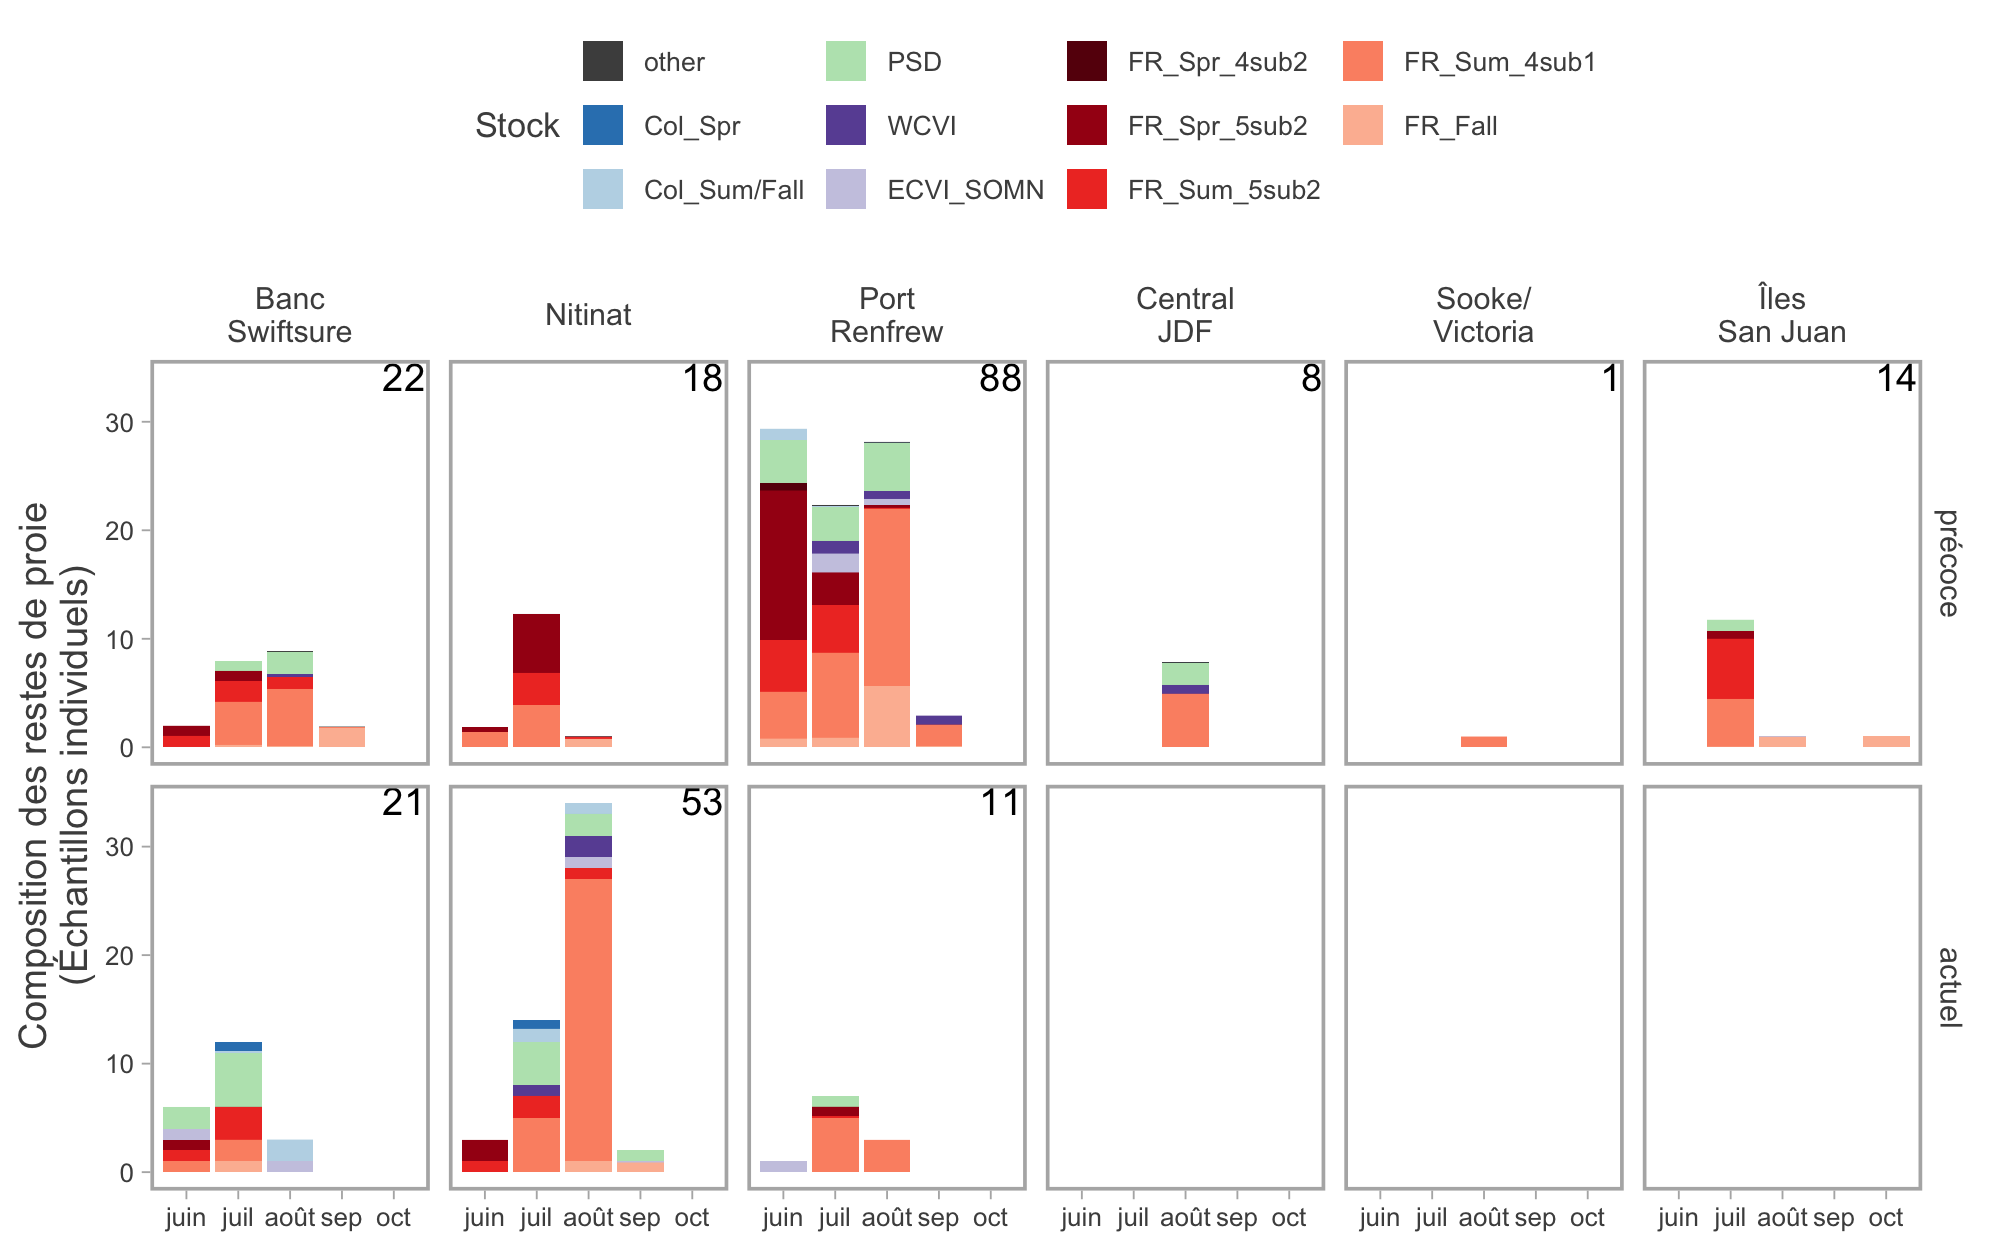
\includegraphics[width=5in]{figs/monthly_comp_bar.png}}{Figure \ref{fig:bar-diet}}
    \caption{Composition mensuelle des stocks de saumon quinnat dans les échantillons de restes de proies des ÉRES. Les strates (colonnes) correspondent aux domaines spatiaux de la Figure \ref{fig:sampling-map}. L'axe des Y représente le nombre d'échantillons collectés dans un mois-strate-période d'échantillonnage donnés. Les chiffres dans le coin supérieur droit de chaque panneau représentent la taille totale de l'échantillon dans chaque strate et période.}
    \label{fig:bar-diet}
\end{figure}

La probabilité que les échantillons d'origine d'écloserie puissent être identifiés de manière fiable dans les restes de proies était relativement faible car les taux de marquage TPB n'excédaient pas 80\% dans de nombreuses écloseries jusqu'à l'année de ponte 2015 ou plus tard (Figure \ref{fig:pbt-coverage}). Six échantillons de restes de proies appartenaient à des populations et des années de ponte avec un taux de marquage TPB supérieur à 80\%. De ceux-ci, trois ont été identifiés selon le stock basé sur le TPB--deux du ruisseau Robertson (COIV) et un de l'écloserie Chilliwack (Fraser automne) respectivement. Quatre autres échantillons de restes de proies ont été identifiés selon le stock basé sur le TPB, mais provenaient d'années population-ponte avec des taux de marquage inférieurs à 80\%--un individu chacun des écloseries Capilano (COIV-SOMN), Puntledge (COIV-SOMN), Big Qualicum (COIV-SOMN), et Chilliwack. Un échantillon de proie a été identifié avec une grande certitude (>99\%) comme provenant de la rivière Nitinat (une population COIV avec un taux PHOS >75\% durant plusieurs années) durant une année avec un faible taux TPB et a donc une probabilité raisonnablement élevée d'être d'origine d'écloserie. Aucun autre échantillon n'avait une assignation de stock qui suggérait une forte probabilité de provenir d'écloseries canadiennes basée sur des taux PHOS élevés (>75\%) durant les années récentes, bien que nous notions que ceci est une technique de classification incertaine.

La majorité des échantillons de restes de proies provenaient de saumons quinnat d'âge océanique-3. Les individus d'âge océanique-4 étaient relativement communs durant la période d'échantillonnage précoce, mais plus rarement observés durant la période actuelle. Peu de saumons quinnat d'âge océanique-2 et aucun d'âge océanique-1 n'ont été identifiés (Figure \ref{fig:bar-age-diet}). L'erreur de vieillissement, ainsi que la variation parmi les échantillons en âge, identité de stock, et date d'échantillonnage ont résulté en une variation additionnelle dans la taille corporelle estimée (Figure \ref{fig:bar-size-diet}). La probabilité que les poissons observés dans les régimes alimentaires étaient plus petits que $65$ cm était très faible à travers tous les mois et strates, tandis que les individus de $65-75$ cm étaient relativement rares. Durant la période précoce, la probabilité que les proies étaient dans la plus grande classe de taille $>85$ cm était relativement élevée, tandis que durant la période actuelle la classe de taille $75-85$ cm avait la plus grande probabilité. Cependant, les différences dans quand et où les échantillons ont été collectés empêchent un test quantitatif pour les changements dans la composition de la taille.

\begin{figure}[H]
    \centering
    \pdftooltip{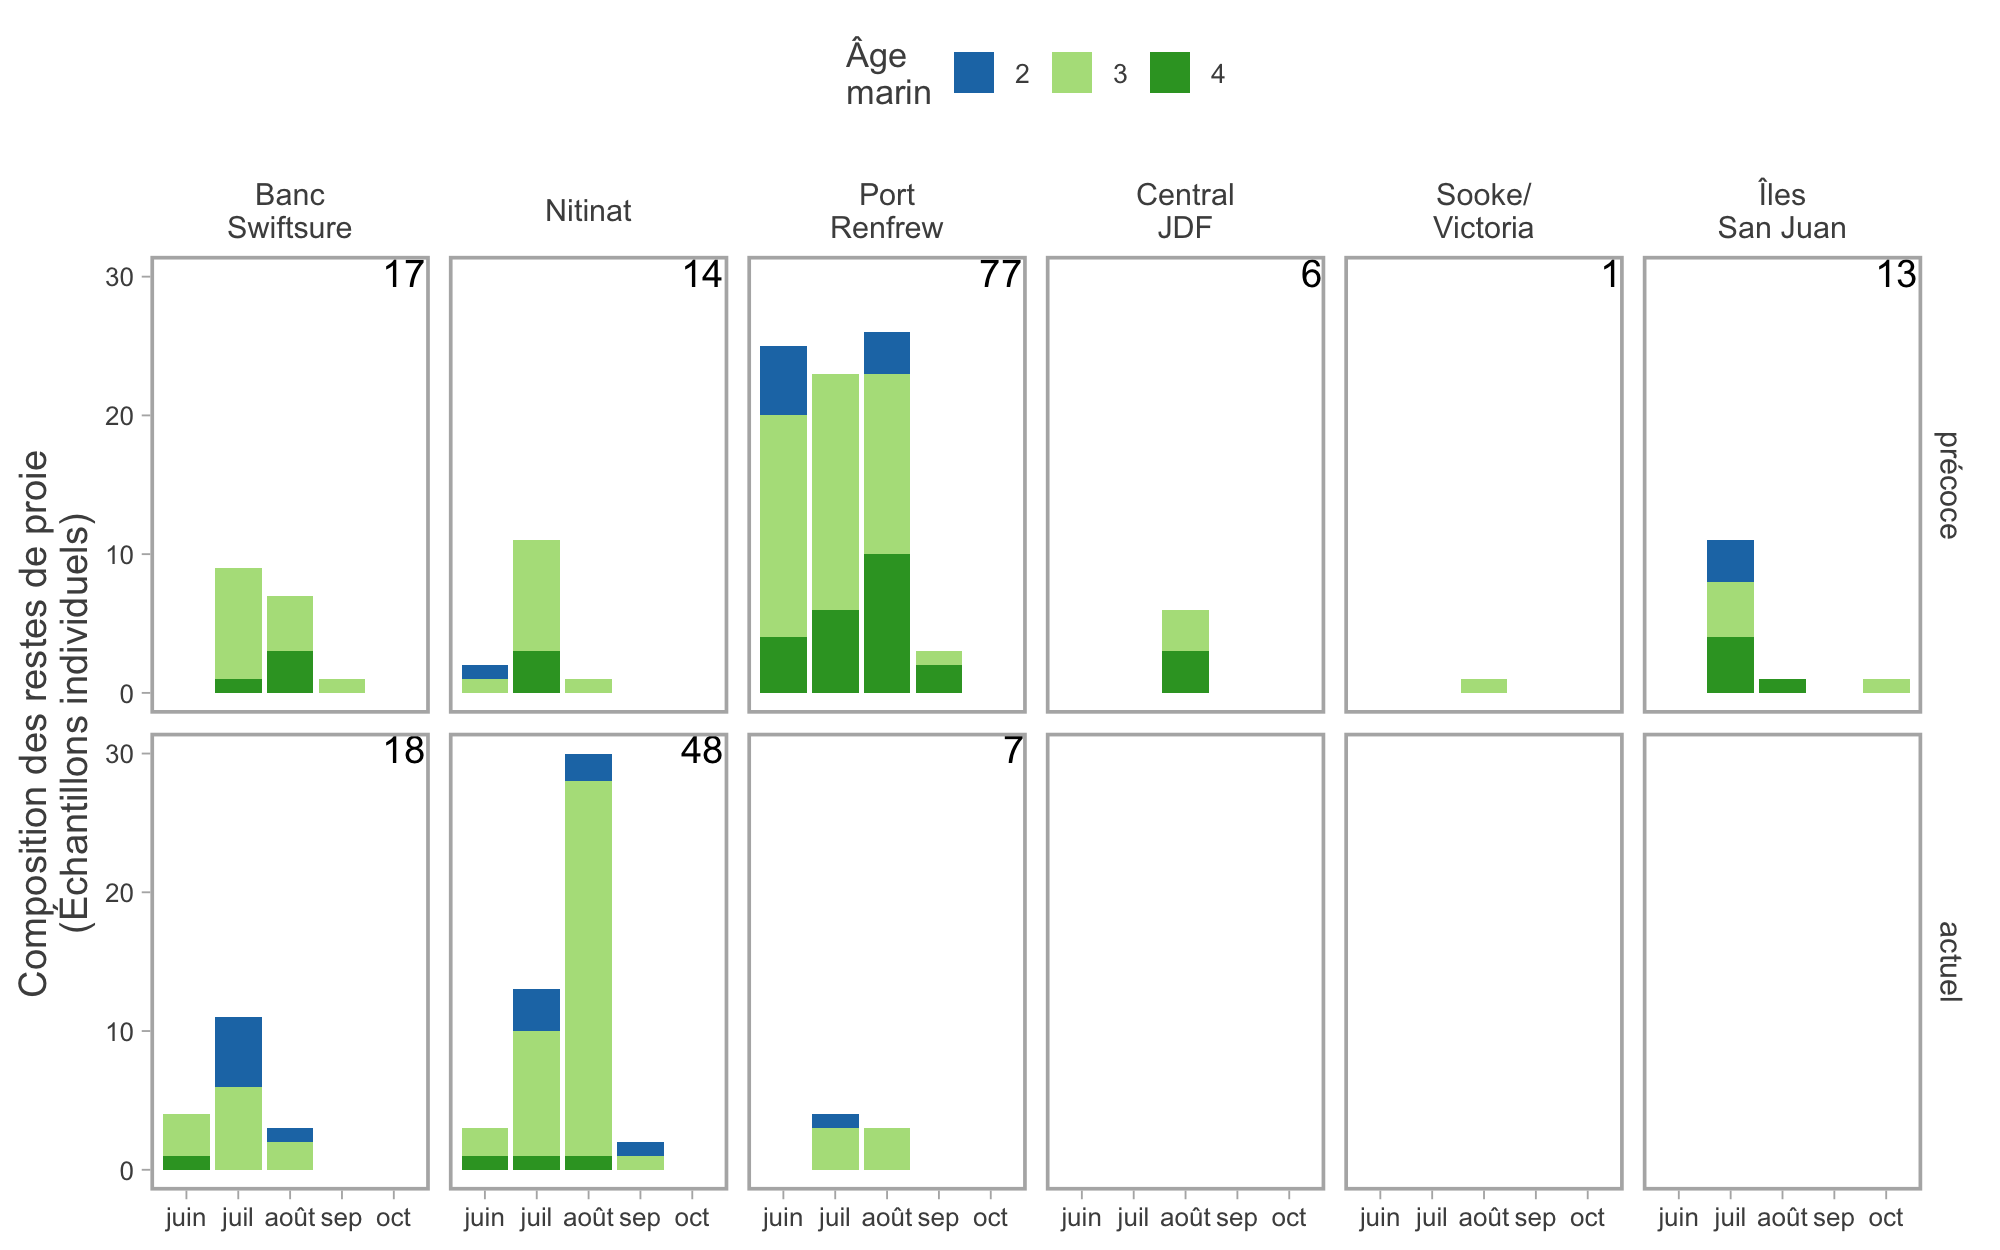
\includegraphics[width=5in]{figs/comp_bar_prey_age.png}}{Figure \ref{fig:bar-age-diet}}
    \caption{Composition mensuelle de l'âge marin du saumon quinnat dans les échantillons de restes de proies des ÉRES. Les données d'âge incorporent l'erreur d'observation associée aux estimations des annuli d'écailles. Les strates (colonnes) correspondent aux domaines spatiaux de la Figure \ref{fig:sampling-map}. L'axe des Y représente le nombre d'échantillons collectés dans un mois-strate-période d'échantillonnage donnés. Les chiffres dans le coin supérieur droit de chaque panneau représentent la taille totale de l'échantillon dans chaque strate et période.}
    \label{fig:bar-age-diet}
\end{figure}

\begin{figure}[H]
    \centering
    \pdftooltip{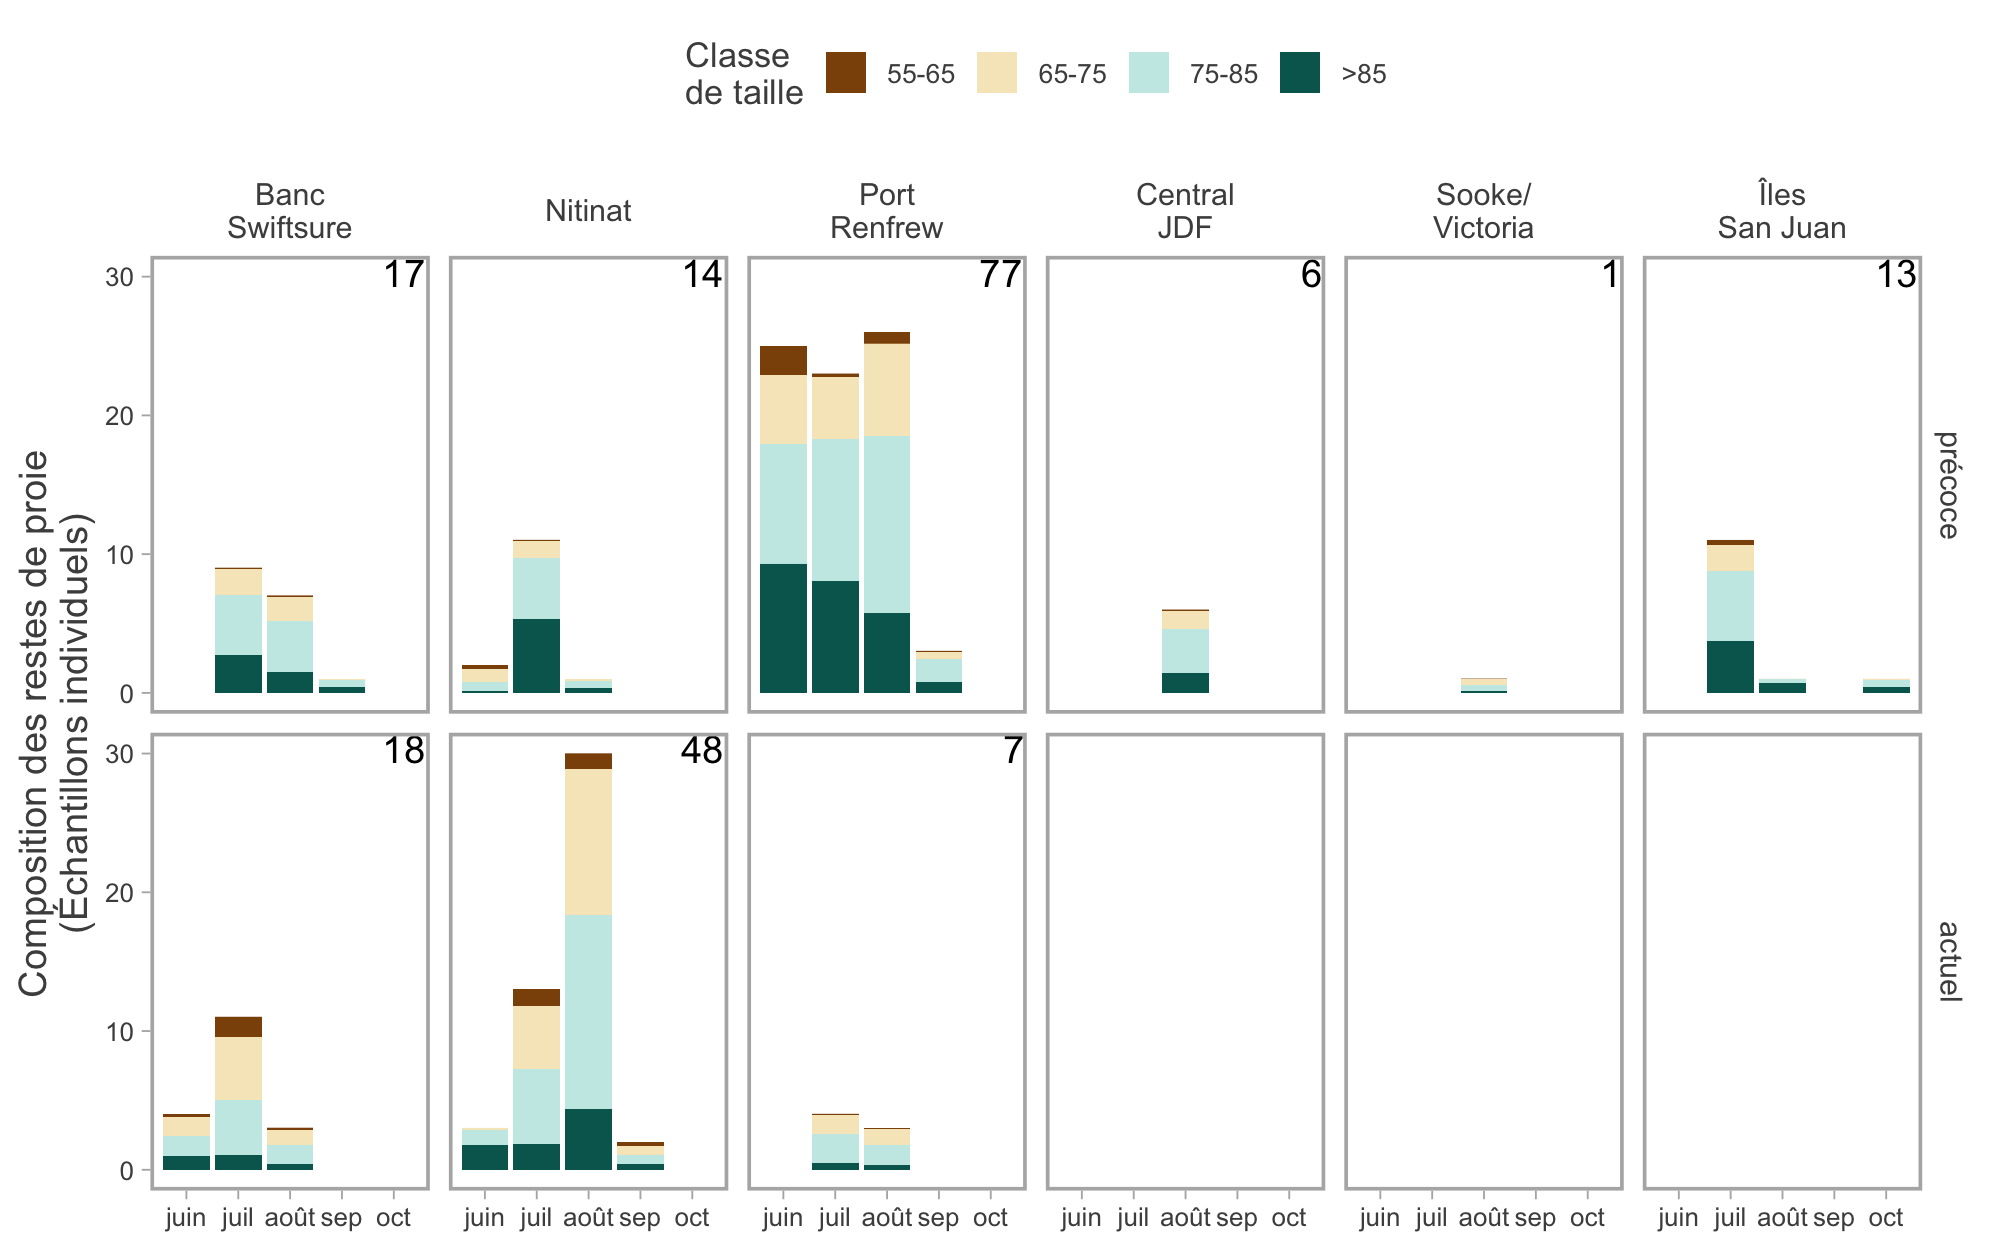
\includegraphics[width=5in]{figs/comp_bar_prey_size.png}}{Figure \ref{fig:bar-size-diet}}
    \caption{Composition mensuelle des classes de taille du saumon quinnat dans les échantillons de restes de proies des ÉRES basée sur les prédictions des modèles taille-selon-l'âge spécifiques aux saisons (Annexe \ref{size-at-age}). Les strates (colonnes) correspondent aux domaines spatiaux de la Figure \ref{fig:sampling-map}. L'axe des Y représente le nombre d'échantillons collectés dans un mois-strate-période d'échantillonnage donnés. Les chiffres dans le coin supérieur droit de chaque panneau représentent la taille totale de l'échantillon dans chaque strate et période.}
    \label{fig:bar-size-diet}
\end{figure}

\subsection{Pêches récréatives de saumon quinnat}

\subsubsection{Composition des stocks}

Il y avait 8 000 échantillons de saumon quinnat qui ont été collectés de saumons quinnat qui étaient (a) plus grands que 55 cm de longueur à la fourche, (b) capturés entre les zones à l'ouest du détroit Juan de Fuca et les îles Gulf du sud de 2014 à 2023, et (c) identifiés selon le stock. La majorité des échantillons de pêche récréative ont été collectés durant les mois d'été d'emplacements à l'intérieur des strates du banc Swiftsure, Port Renfrew, et Victoria/Sooke (Figures \ref{fig:bar-rec-summer}, \ref{fig:bar-rec-full}). Dans les strates où les échantillons de pêche étaient disponibles à travers toutes les saisons, la composition des stocks a transité d'être dominée par le stock Puget Sound entre novembre et mai vers un assemblage plus mixte durant l'été (Figure \ref{fig:bar-rec-full}).

\begin{figure}[H]
    \centering
    \pdftooltip{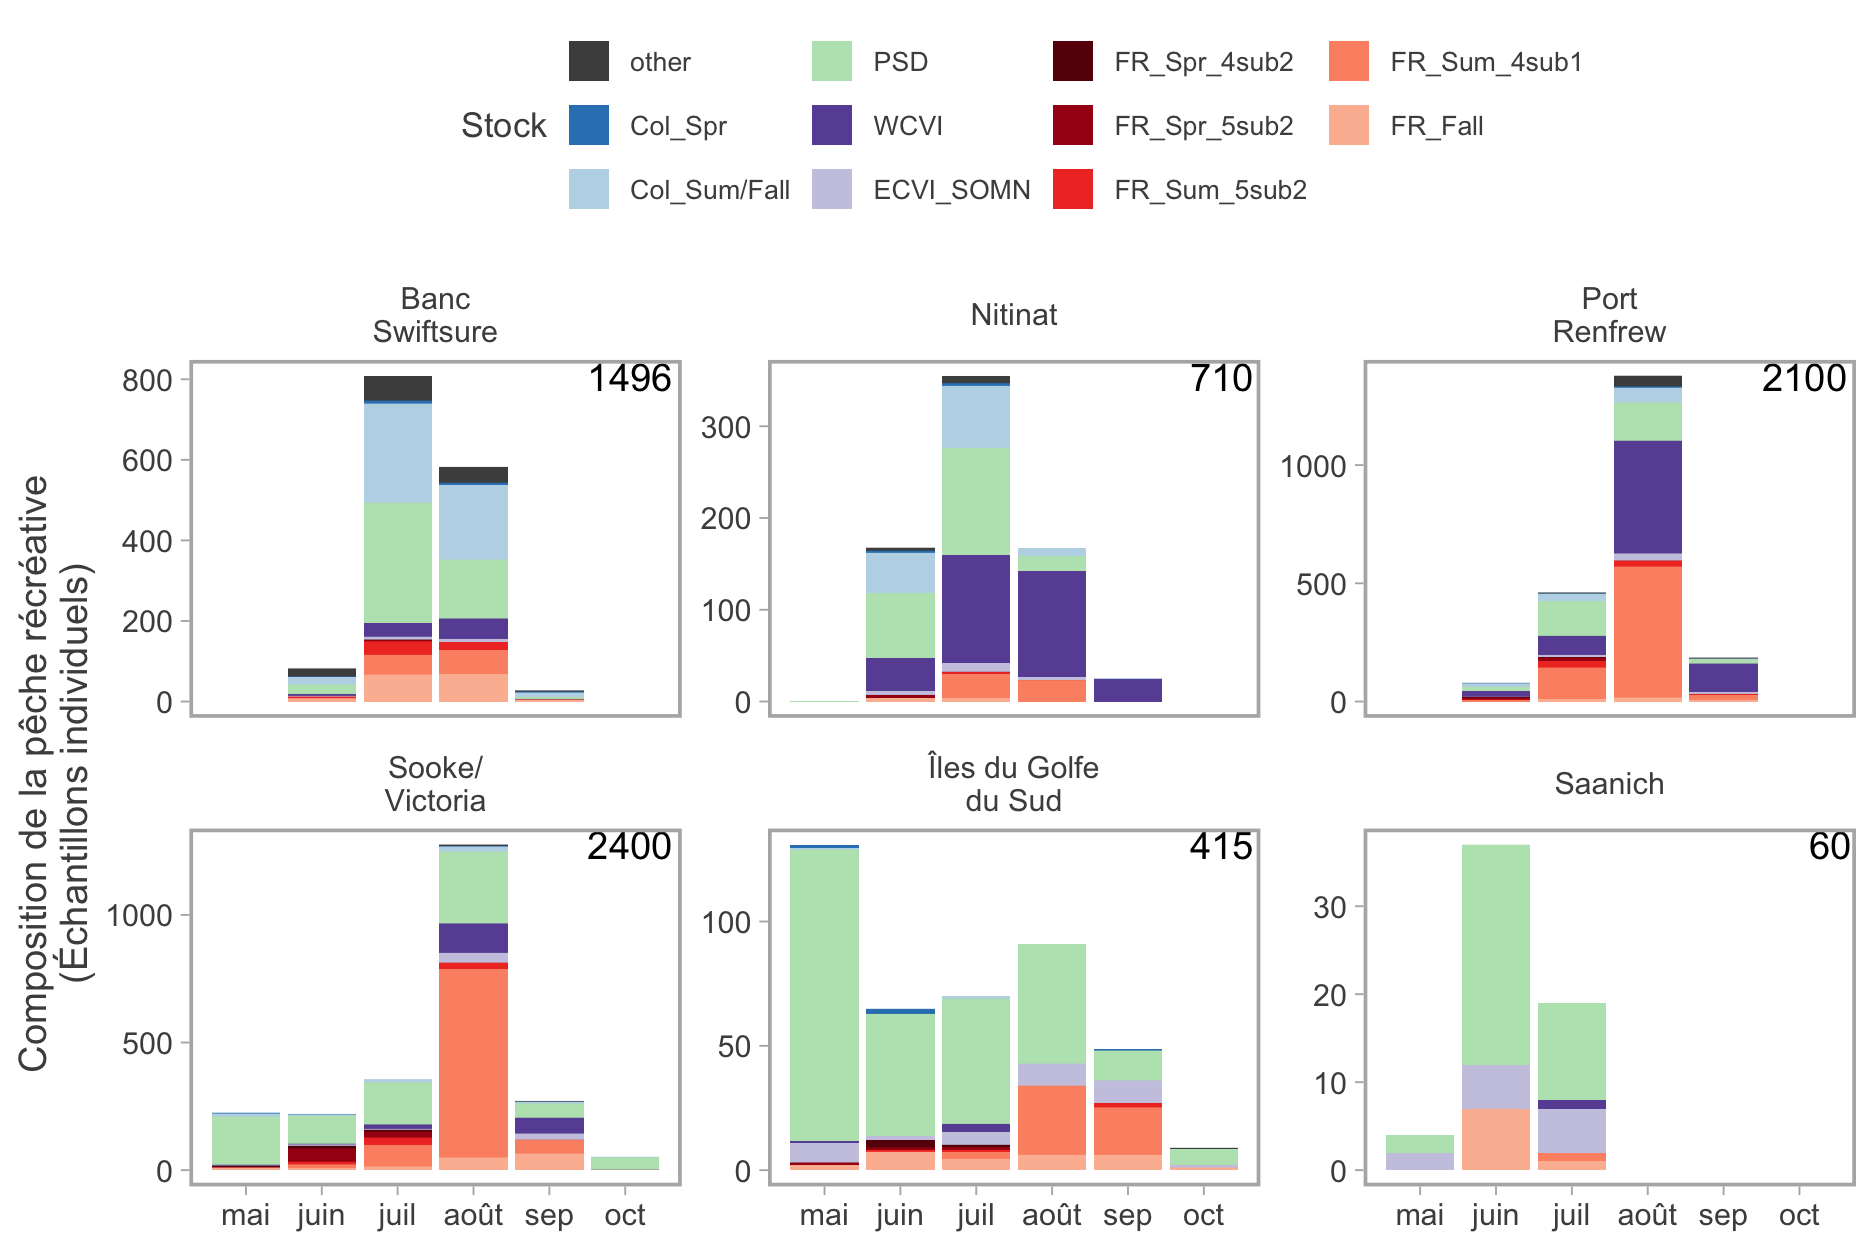
\includegraphics[width=5in]{figs/rec_monthly_comp_bar_summer.png}}{Figure \ref{fig:bar-rec-summer}}
    \caption{Composition mensuelle (mai-octobre) des stocks d'échantillons de pêche récréative de saumon quinnat. Les strates (panneaux) correspondent aux domaines spatiaux de la Figure \ref{fig:sampling-map}. L'axe des Y représente le nombre d'échantillons collectés dans un mois et une strate spatiale donnés. Les chiffres dans le coin supérieur droit de chaque panneau représentent la taille totale de l'échantillon dans chaque strate.}
    \label{fig:bar-rec-summer}
\end{figure}

La moyenne et la variance de la longueur à la fourche différaient parmi les stocks (Figure \ref{fig:density-fl}). Les poissons COIV, Fraser printemps $5_2$, été $5_2$, et été $4_1$ étaient typiquement plus grands (longueurs médianes entre 75 et 80 cm), tandis que les stocks Puget Sound et COIV-SOMN étaient relativement plus petits (longueurs médianes inférieures à 70 cm). Le stock Fraser rivière été $4_1$ avait une distribution de taille plus homogène (CV=0,09) que les stocks Puget Sound, Columbia rivière printemps, Fraser rivière automne, et COIV-SOMN (CV=0,12-0,13).

\begin{figure}[H]
    \centering
    \pdftooltip{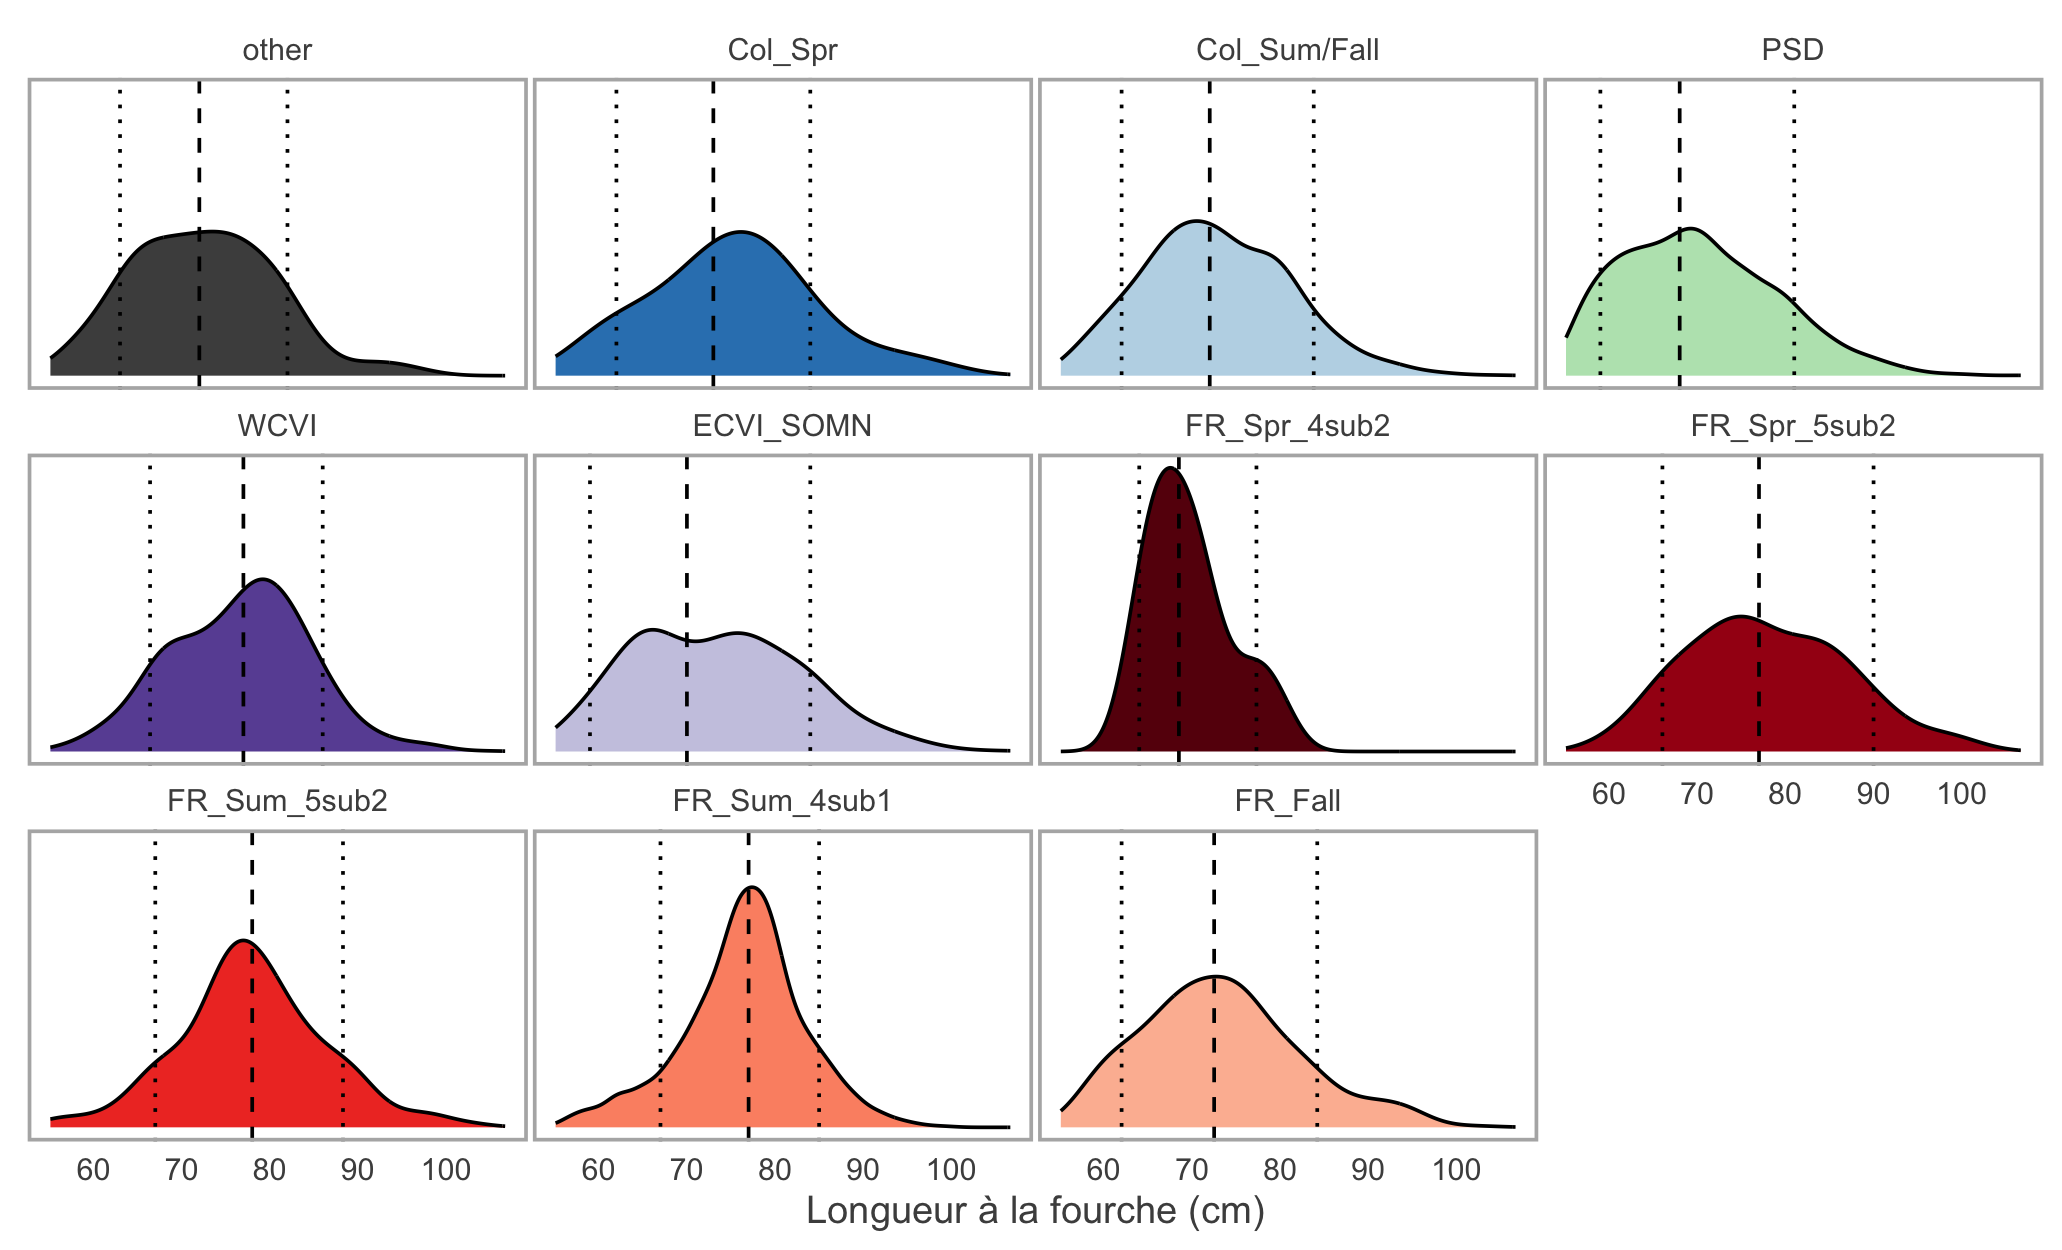
\includegraphics[width=5in]{figs/size_density.png}}{Figure \ref{fig:density-fl}}
    \caption{Estimations de densité par noyau de la longueur à la fourche (mm) spécifique aux stocks observée d'échantillons de pêche récréative de saumon quinnat (collectés entre mai-octobre). Les lignes verticales représentent les médianes spécifiques aux stocks (pointillées) et les intervalles du 80e percentile (ponctuées). Notez que les échantillons plus petits que 55 cm sont exclus. Notez que l'échelle de l'axe des y diffère parmi les strates.}
    \label{fig:density-fl}
\end{figure}

Notre modèle statistique a capturé la variabilité saisonnière, spatiale, et interannuelle dans l'abondance relative des stocks de saumon quinnat, tout en tenant compte de l'effort d'échantillonnage inégal. Les stocks de saumon quinnat différaient non seulement dans l'abondance relative moyenne, mais aussi les tendances saisonnières dans l'abondance relative. L'abondance relative des stocks juvéniles Fraser (c.-à-d., printemps $4_2$, printemps $5_2$, et été $5_2$) a décliné au cours de l'été, tandis que l'abondance Puget Sound a décliné durant l'été puis s'est rétablie durant septembre (Figure \ref{fig:season-pred-rec}). Les stocks Fraser été $4_1$ et COIV ont tous deux atteint l'abondance maximale à la fin de l'été, mais avec des pics à plusieurs semaines d'intervalle, tandis que le stock Fraser automne a atteint un pic à la fin septembre (Figure \ref{fig:season-pred-rec}).

\begin{figure}[H]
    \centering
    \pdftooltip{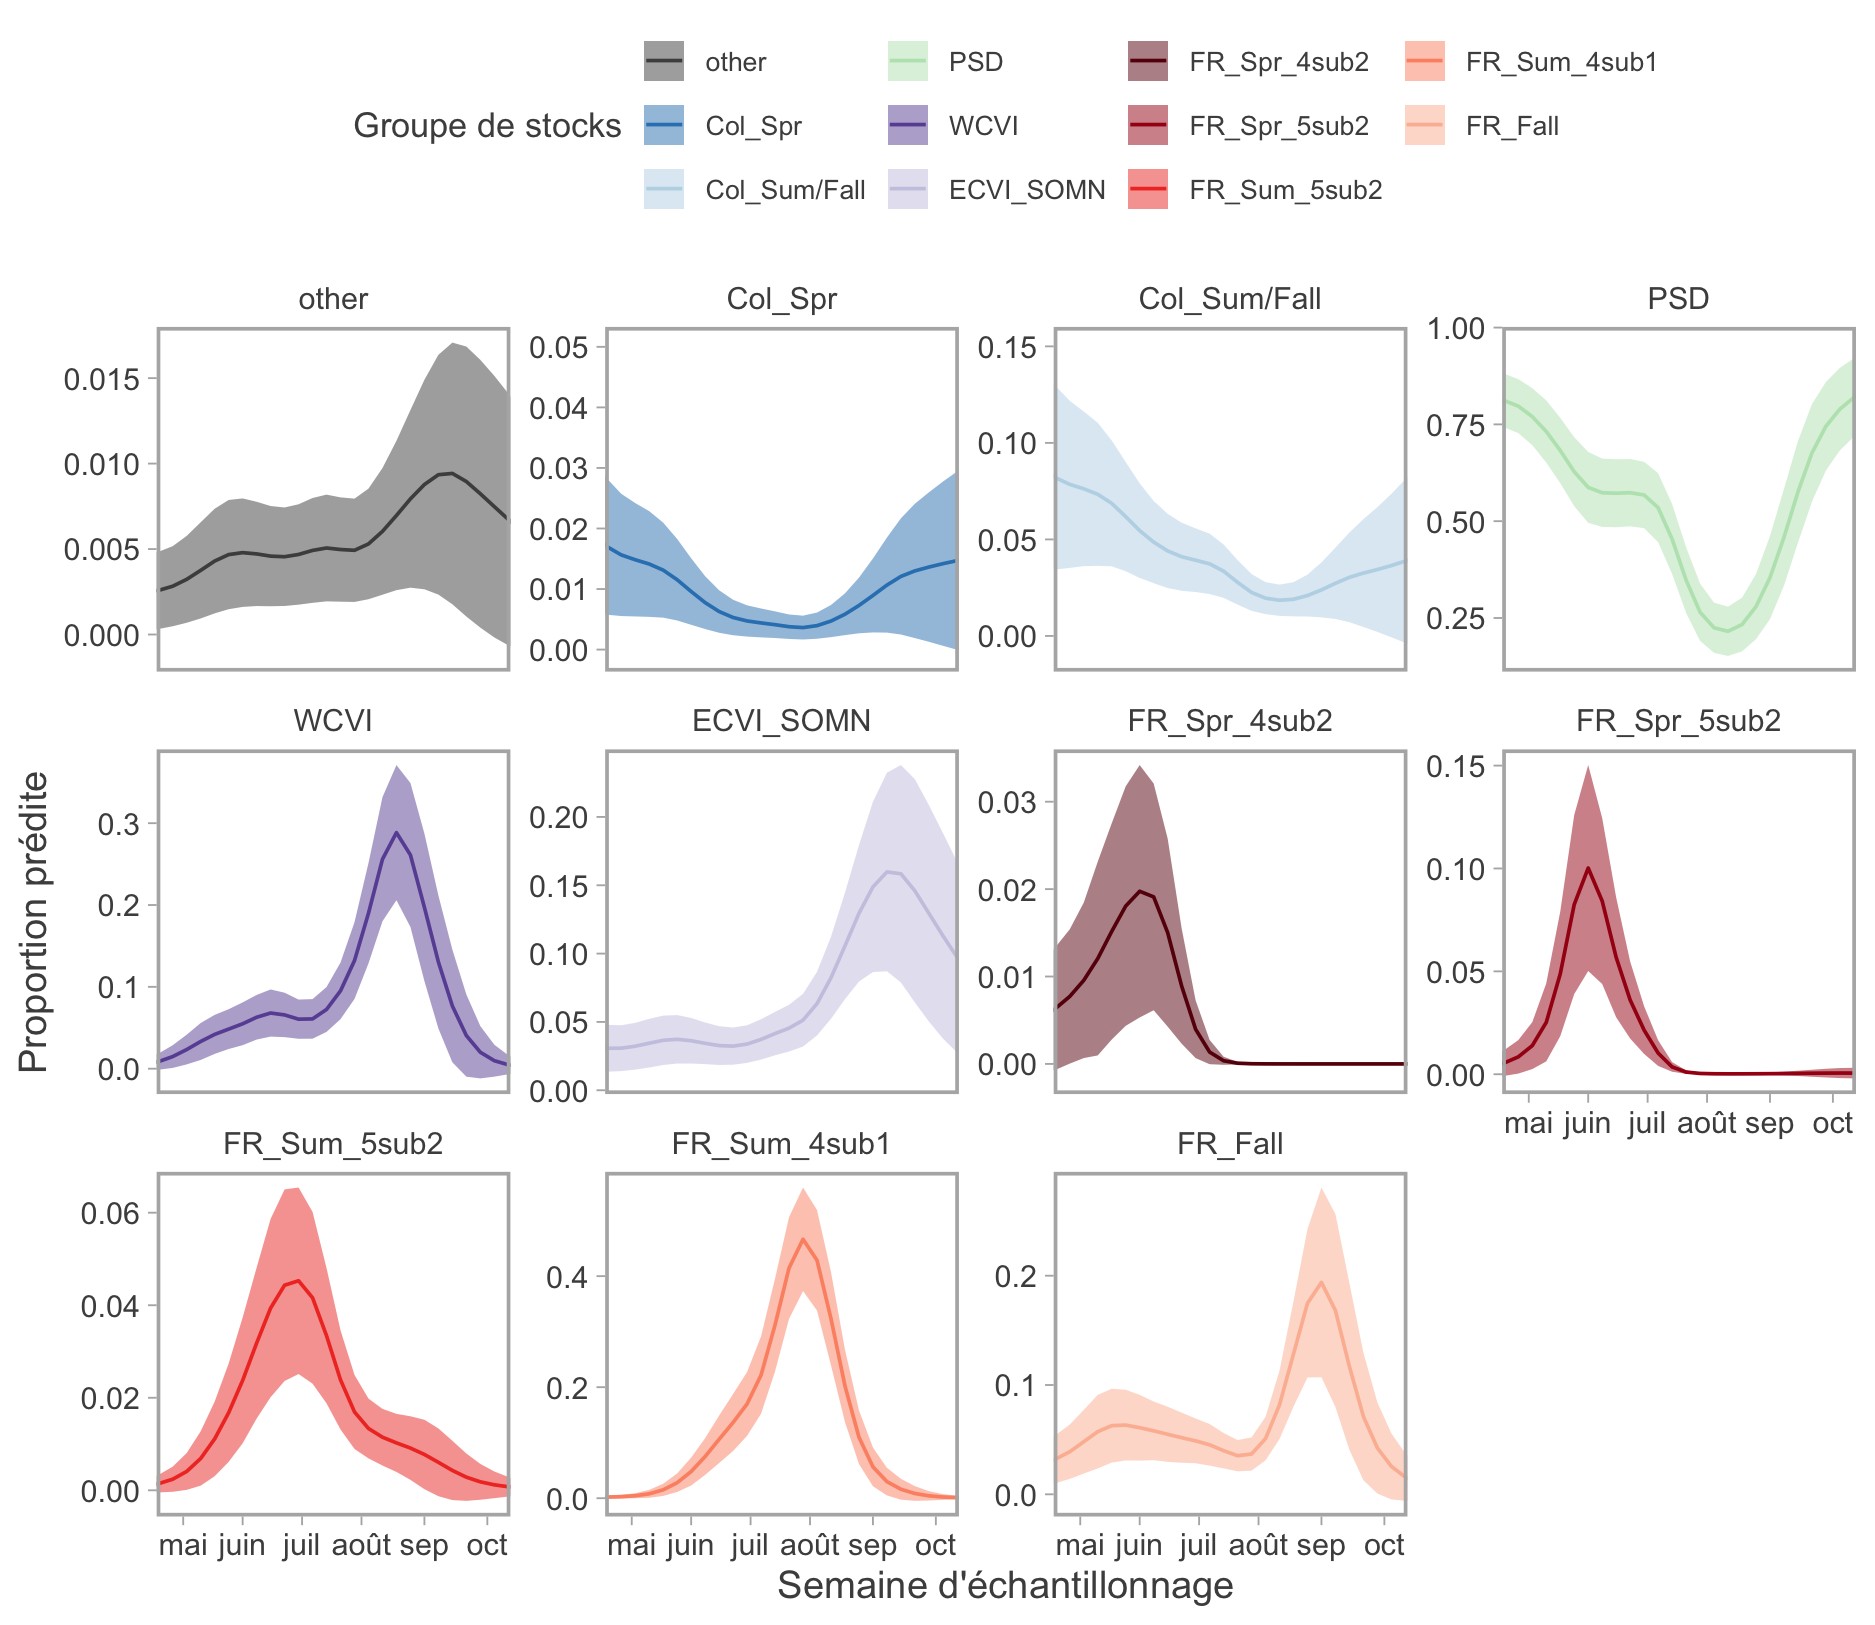
\includegraphics[width=5in]{figs/season_preds_chinook.png}}{Figure \ref{fig:season-pred-rec}}
    \caption{Composition saisonnière moyenne prédite des stocks, basée sur un modèle ajusté aux échantillons de pêche récréative, de mai à octobre. Le ruban représente l'intervalle de confiance à 95\% de la prédiction moyenne. Les prédictions représentent les effets conditionnels, excluant les covariables spatiales (c.-à-d., représentent l'effet saisonnier moyen à l'intérieur de la zone d'étude). Notez que l'échelle de l'axe des y diffère parmi les stocks.}
    \label{fig:season-pred-rec}
\end{figure}

Les stocks montraient aussi des distributions spatiales uniques. Les stocks 'Autre', Columbia printemps, Columbia été/automne, et Fraser automne étaient à leur abondance la plus élevée près de l'embouchure du détroit Juan de Fuca et du banc Swiftsure, tandis que le stock Puget Sound montrait le patron opposé (Figure \ref{fig:spatial-pred-scaled}). Le stock COIV était concentré près des côtes, particulièrement près du lac Nitinat, tandis que les stocks Fraser printemps $4_2$, printemps $5_2$, été $5_2$, et été $4_1$ étaient les plus abondants au milieu du détroit Juan de Fuca (Figure \ref{fig:spatial-pred-scaled}). Les prédictions non mises à l'échelle soulignent que la composition des stocks, en moyennant parmi les mois de mai à octobre, variait spatialement. Généralement Columbia été/automne et Puget Sound étaient les stocks dominants---le premier sur le banc Swiftsure et le dernier dans le sud du détroit de Georgie (Figure \ref{fig:spatial-pred}). Le stock COIV était dominant dans les emplacements côtiers près du lac Nitinat, tandis que le détroit Juan de Fuca avait une composition de stocks plus équilibrée due à l'abondance relativement élevée du stock Fraser été $4_1$ (Figure \ref{fig:spatial-pred}).

\begin{figure}[H]
    \centering
    \pdftooltip{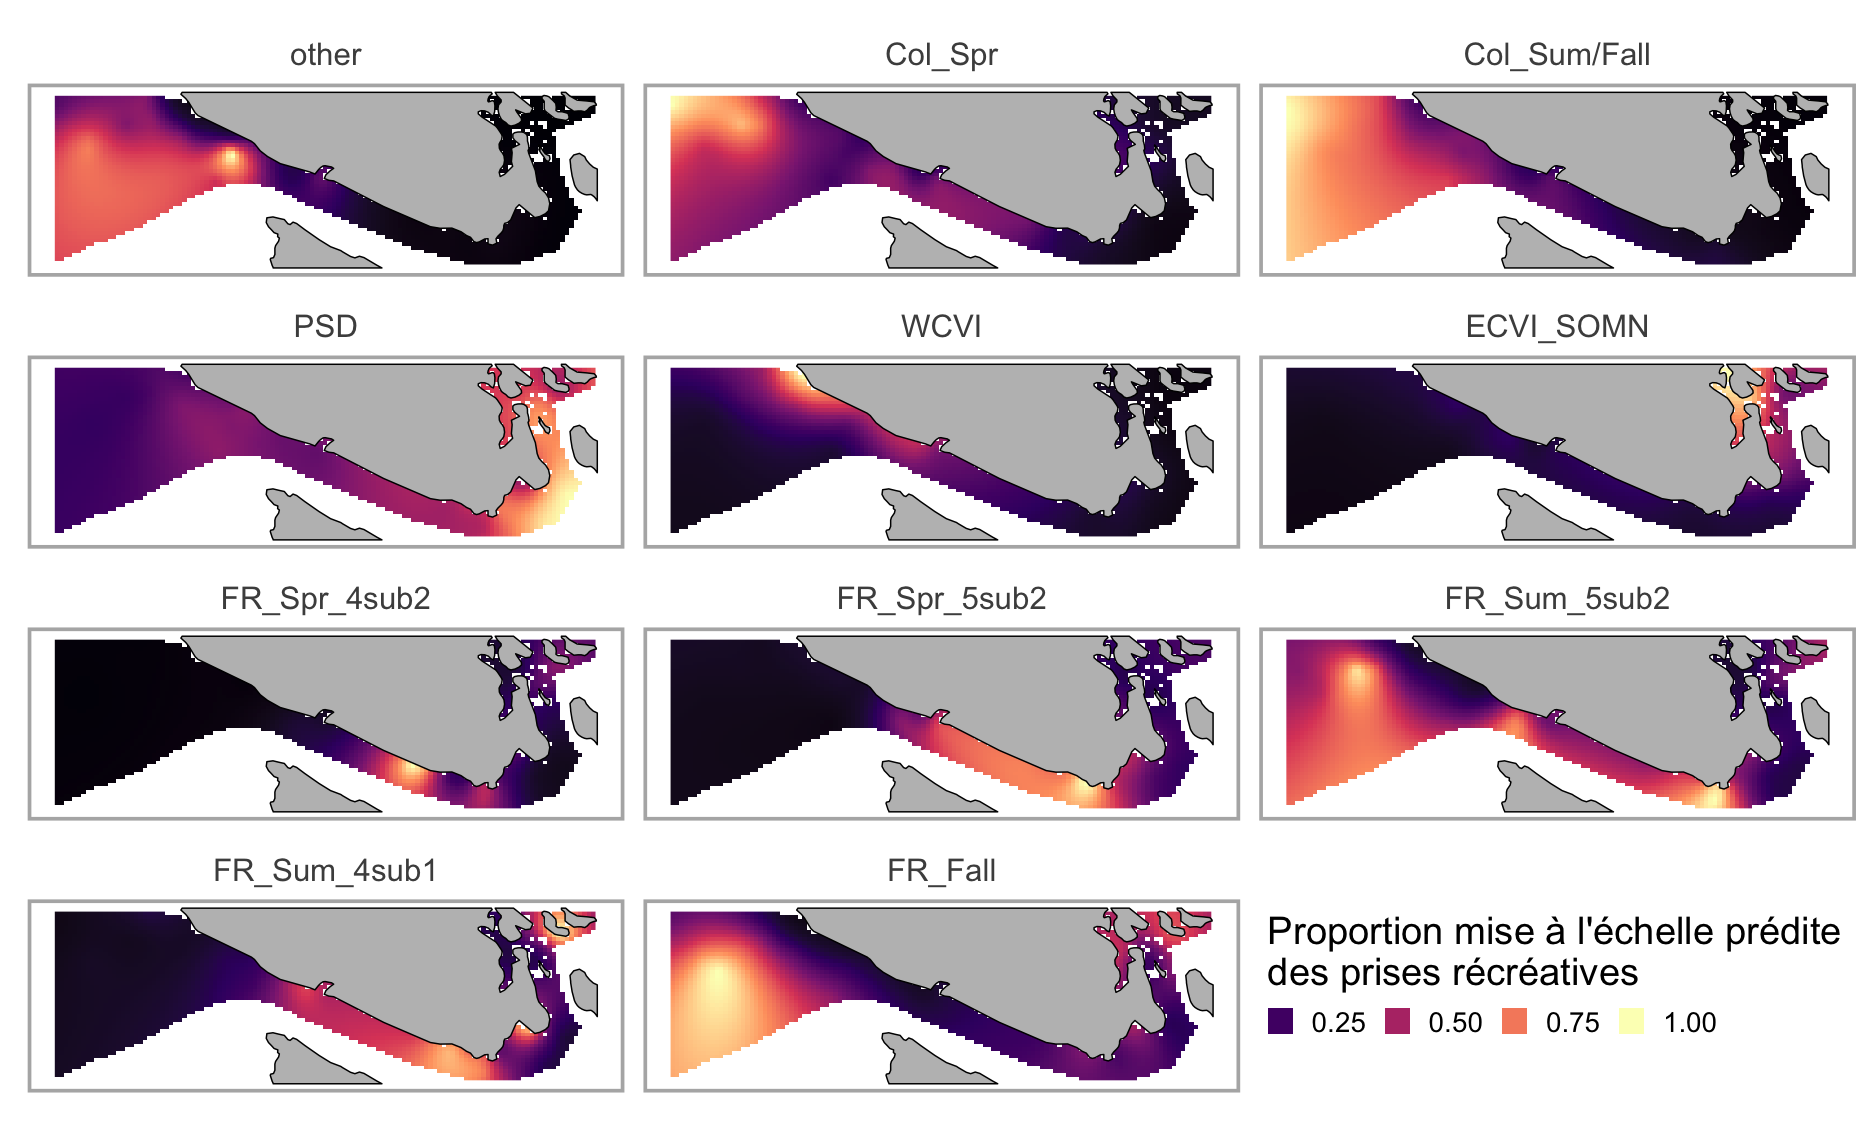
\includegraphics[width=5in]{figs/spatial_preds_scaled.png}}{Figure \ref{fig:spatial-pred-scaled}}
    \caption{Variation spatiale dans la composition moyenne prédite des stocks mise à l'échelle à travers la portion canadienne du détroit Juan de Fuca et le sud du détroit de Georgie basée sur les échantillons de pêche récréative. Les prédictions sont des moyennes spécifiques aux stocks pour mai à octobre et ont été mises à l'échelle relativement à la prédiction maximale à l'intérieur d'un stock pour souligner les différences spécifiques aux stocks. Une valeur de un (zéro) indique l'emplacement où un stock était à son abondance prédite maximale (minimale).}
    \label{fig:spatial-pred-scaled}
\end{figure}

\begin{figure}[H]
    \centering
    \pdftooltip{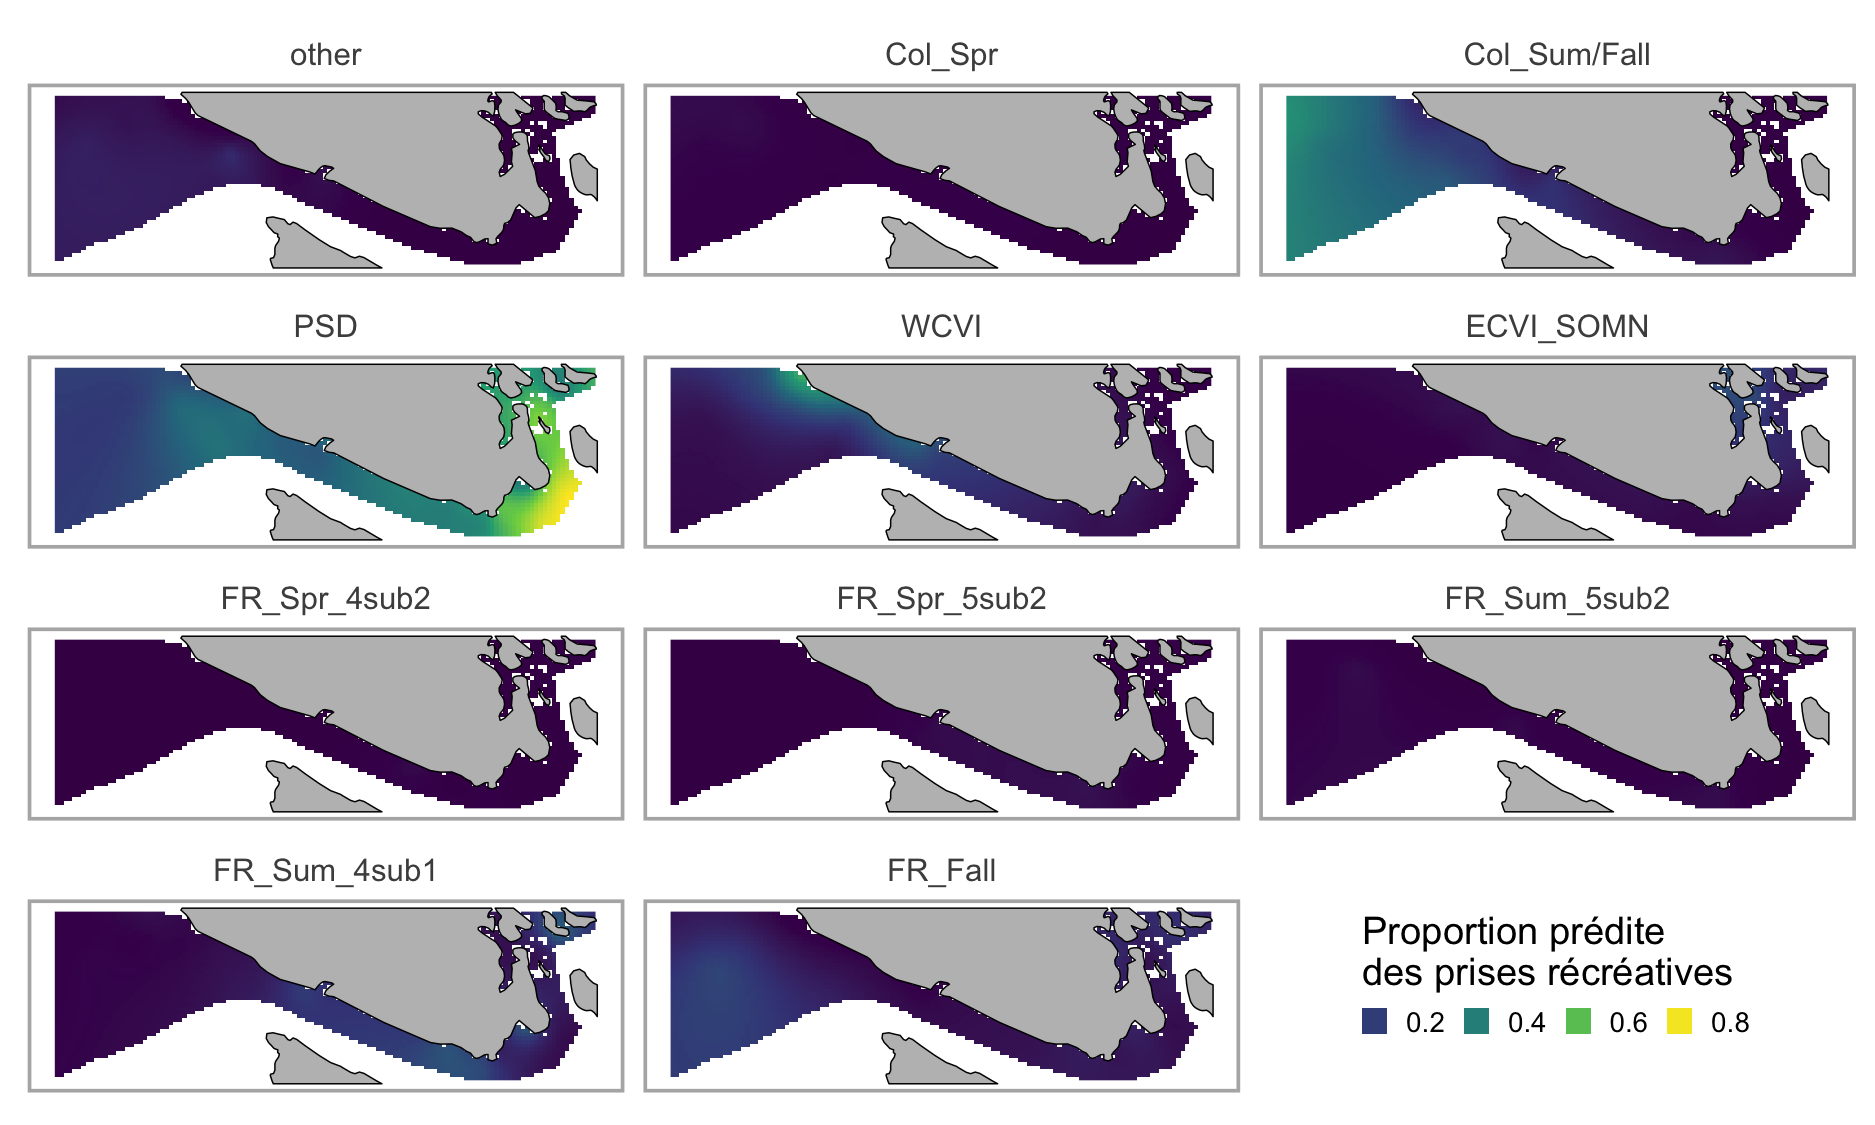
\includegraphics[width=5in]{figs/spatial_preds.png}}{Figure \ref{fig:spatial-pred}}
    \caption{Variation spatiale dans la composition moyenne prédite des stocks à travers la portion canadienne du détroit Juan de Fuca et le sud du détroit de Georgie basée sur les échantillons de pêche récréative. Les prédictions sont des moyennes spécifiques aux stocks pour mai à octobre. Une valeur de un (zéro) indique qu'un stock représentait 100\% (0\%) de l'échantillon moyen prédit.}
    \label{fig:spatial-pred}
\end{figure>

Les prédictions saisonnières de la composition moyenne des stocks pour des strates spécifiques soulignent simultanément la variabilité spatiale et temporelle dans l'abondance relative de différents stocks (Figure \ref{fig:stacked-rec}). Près du banc Swiftsure, les stocks Puget Sound et Columbia été/automne constituaient plus de 90\% de la capture en juin, mais les stocks Fraser été $4_1$ et COIV constituaient des composantes significatives de la capture au fur et à mesure que l'été progressait. Nitinat montrait un patron similaire, sauf avec une contribution beaucoup plus grande d'individus COIV, particulièrement en août et septembre quand ce stock constituait plus de 50\% de la capture. Les strates Port Renfrew et Sooke/Victoria montraient la plus grande contribution de poissons appartenant aux stocks de la rivière Fraser. Les poissons en route vers Fraser constituaient approximativement 50\% de la capture en août, prédominamment le stock été $4_1$, mais les stocks avec une chronologie de montaison plus précoce étaient quelque peu communs en juin. Les strates Port Renfrew et Sooke/Victoria différaient principalement dans la proportion des stocks Puget Sound et COIV. Les strates des îles Gulf du sud montraient une composition de stocks similaire à Sooke/Victoria, mais incluaient plus d'individus COIV/SOMN.

\begin{figure}[H]
    \centering
    \pdftooltip{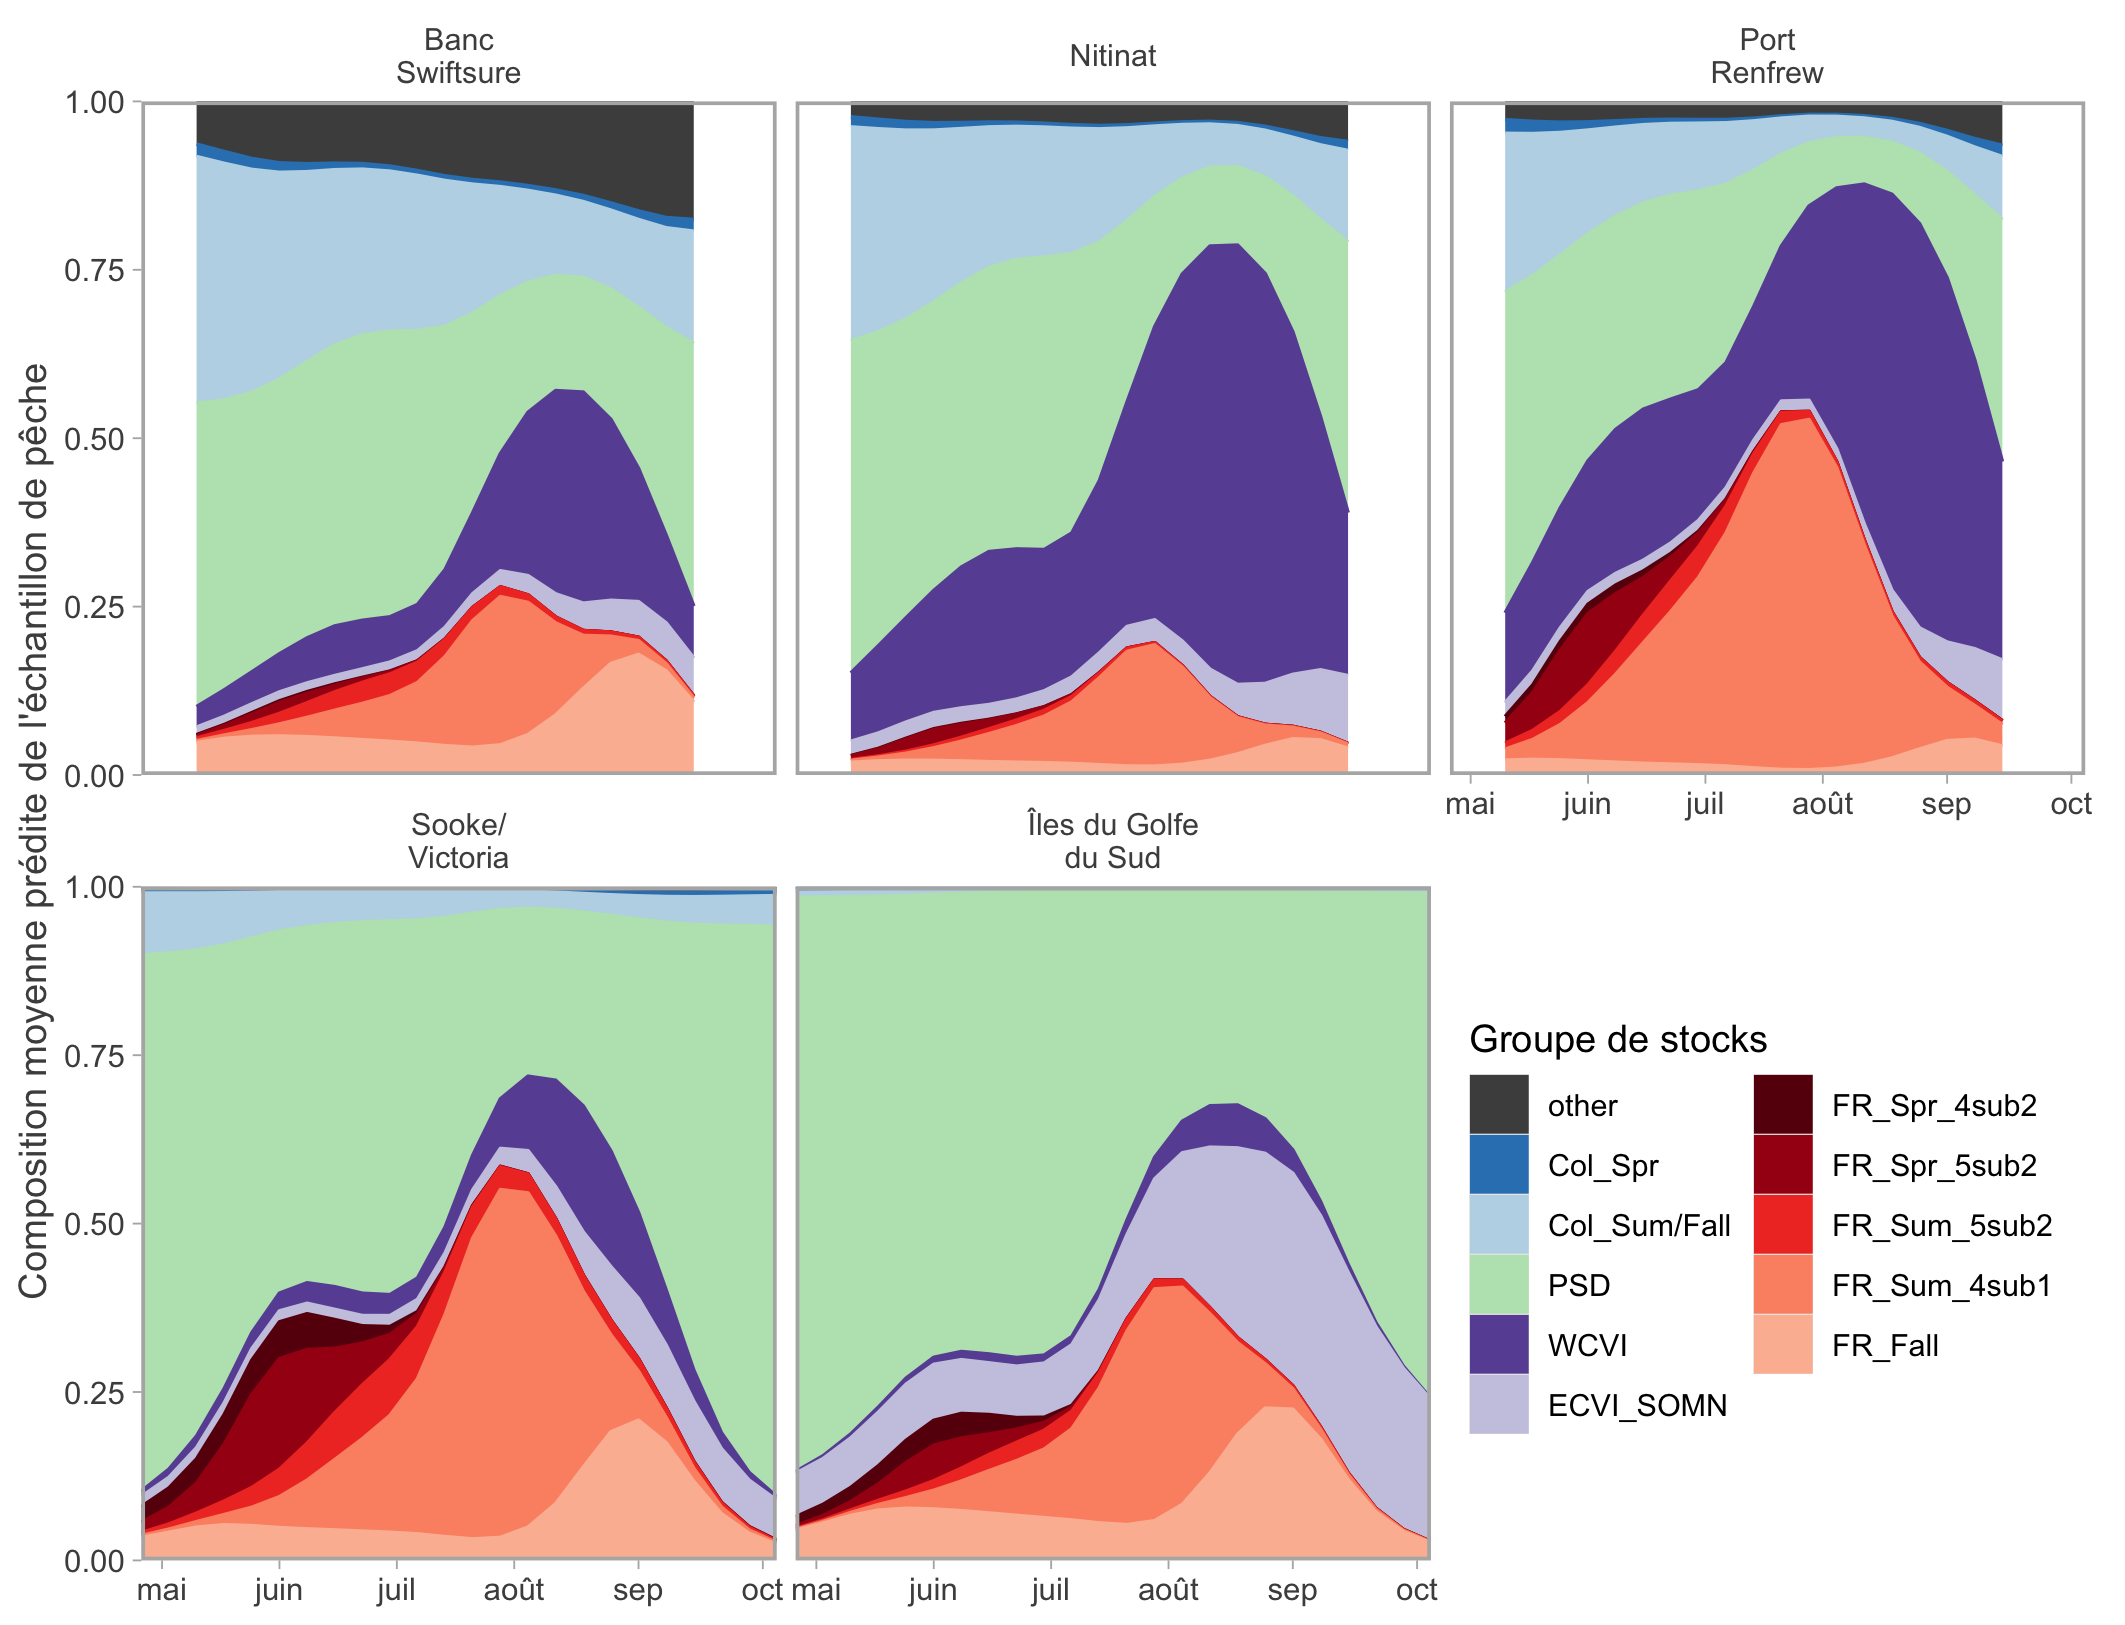
\includegraphics[width=5in]{figs/smooth_preds_chinook_stacked.png}}{Figure \ref{fig:stacked-rec}}
    \caption{Composition saisonnière moyenne prédite des stocks durant les mois d'été parmi cinq strates spatiales basée sur les échantillons de pêche récréative. Les prédictions ont été estimées en utilisant les emplacements (représentés par un « x ») à l'intérieur de chaque domaine spatial de la Figure \ref{fig:sampling-map} et excluent la variabilité interannuelle. Saanich non montré en raison de données limitées en juillet et août, ainsi que son emplacement à l'extérieur de l'habitat essentiel des ÉRES.}
    \label{fig:stacked-rec}
\end{figure}

La variabilité interannuelle dans l'abondance relative différait parmi les stocks et les emplacements spatiaux. Les stocks Columbia rivière printemps, Puget Sound, et COIV étaient relativement stables comparés aux stocks restants (Figure \ref{fig:smooth-pred-rec-year}). Par exemple, la proportion moyenne prédite de l'échantillon appartenant au Fraser rivière été $5_2$ à Sooke/Victoria en juillet variait de 4,6\% à 17,7\% parmi les années.

Les résidus du modèle ajusté étaient appropriément distribués (Figure \ref{fig:qqplot-stock}) et les vérifications prédictives postérieures ont confirmé que la composition moyenne simulée des stocks, tenant compte de la variance résiduelle, était généralement similaire à la composition observée des stocks (Figures \ref{fig:posterior-stock1}, \ref{fig:posterior-stock2}, \ref{fig:posterior-stock3}). Cependant la nature hiérarchique des modèles spatio-temporels, qui était nécessaire pour générer des prédictions pour un nombre relativement grand de stocks, a résulté en un rétrécissement qui tirait les observations individuelles vers la moyenne globale. En conséquence, les observations des strates avec relativement peu d'échantillons, comme Saanich, et les combinaisons stock-strates avec des patrons saisonniers fortement non-linéaires (p. ex., COIV à Nitinat) déviaient le plus fortement des prédictions du modèle.

\subsubsection{Composition de la taille}

Nous avons évalué la composition de la taille en utilisant les données de 10 651 saumons quinnat, plus grands que 55 cm de longueur à la fourche. Bien que la taille totale de l'échantillon pour l'analyse de composition de la taille était plus grande, plusieurs échantillons étaient partagés avec l'ensemble de données de composition des stocks décrit précédemment, résultant en une distribution saisonnière et spatiale similaire d'échantillons. Les individus plus petits que 75 cm étaient relativement communs dans les strates du banc Swiftsure, des îles Gulf du sud, et de Saanich, tandis que les classes de taille plus grandes étaient les plus abondantes à Nitinat et Port Renfrew (Figure \ref{fig:bar-rec-summer-size}). Dans les strates où les échantillons étaient disponibles à travers toutes les saisons, les poissons plus grands que 75 cm étaient largement absents avant mai et après septembre (Figure \ref{fig:bar-rec-full-size}).

\begin{figure}[H]
    \centering
    \pdftooltip{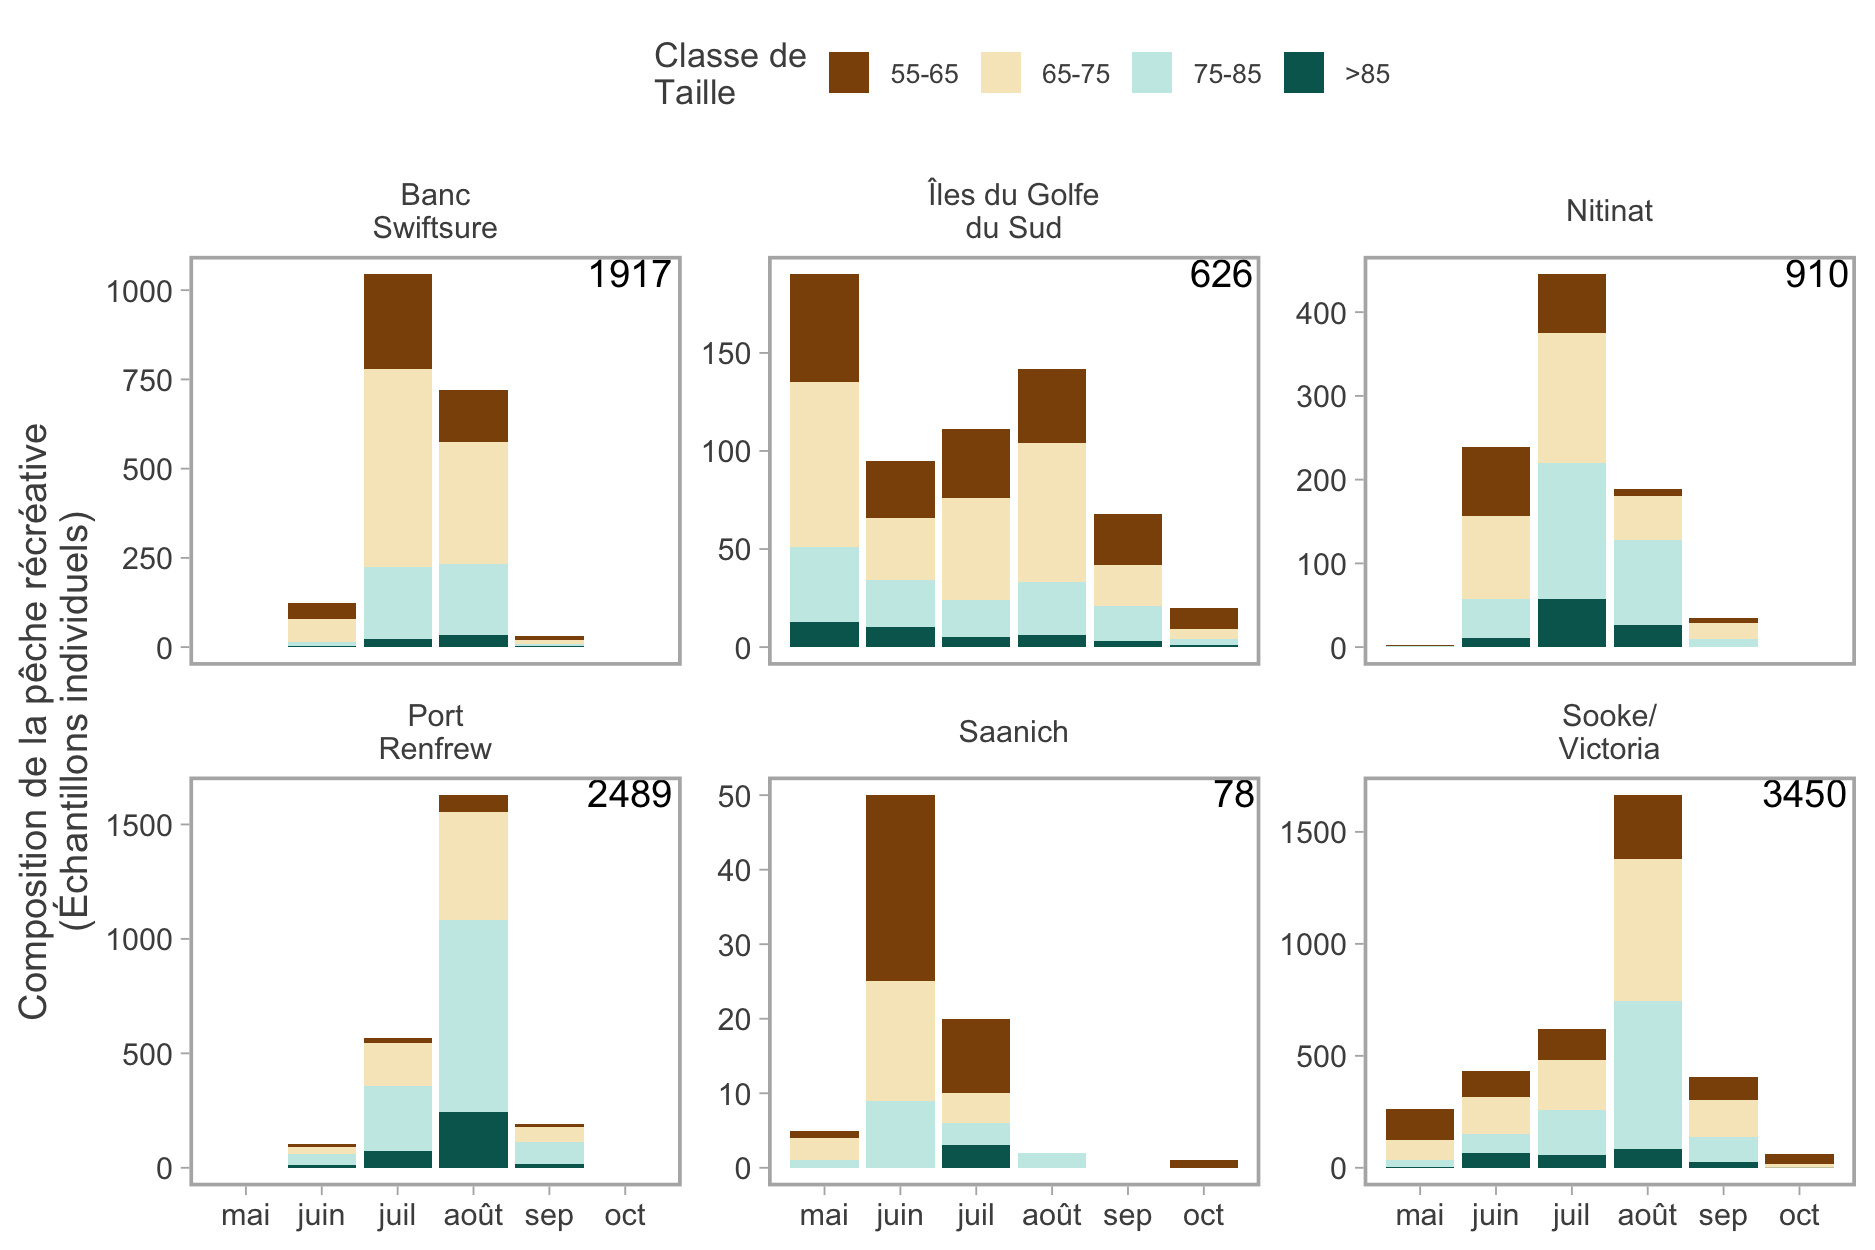
\includegraphics[width=5in]{figs/rec_monthly_size_bar_summer.png}}{Figure \ref{fig:bar-rec-summer-size}}
    \caption{Composition mensuelle de la taille d'échantillons de pêche récréative de saumon quinnat durant les mois d'été. Les strates (panneaux) correspondent aux domaines spatiaux de la Figure \ref{fig:sampling-map}. L'axe des Y représente le nombre d'échantillons collectés dans un mois et une strate spatiale donnés (notez que l'échelle diffère parmi les strates). Les chiffres dans le coin supérieur droit de chaque panneau représentent la taille totale de l'échantillon dans chaque strate.}
    \label{fig:bar-rec-summer-size}
\end{figure}

Les classes de taille du saumon quinnat différaient dans l'abondance moyenne et saisonnière (Figure \ref{fig:season-pred-size}). L'abondance relative de la classe de taille 55-65 cm a décliné à travers l'été avant d'augmenter en septembre, tandis que les individus de 75-85 cm étaient les plus abondants à la fin juillet et en août. Les classes de taille 65-75 cm et supérieure à 85 cm étaient relativement plus stables, bien que les deux aient décliné en septembre (Figure \ref{fig:season-pred-size}).

\begin{figure}[H]
    \centering
    \pdftooltip{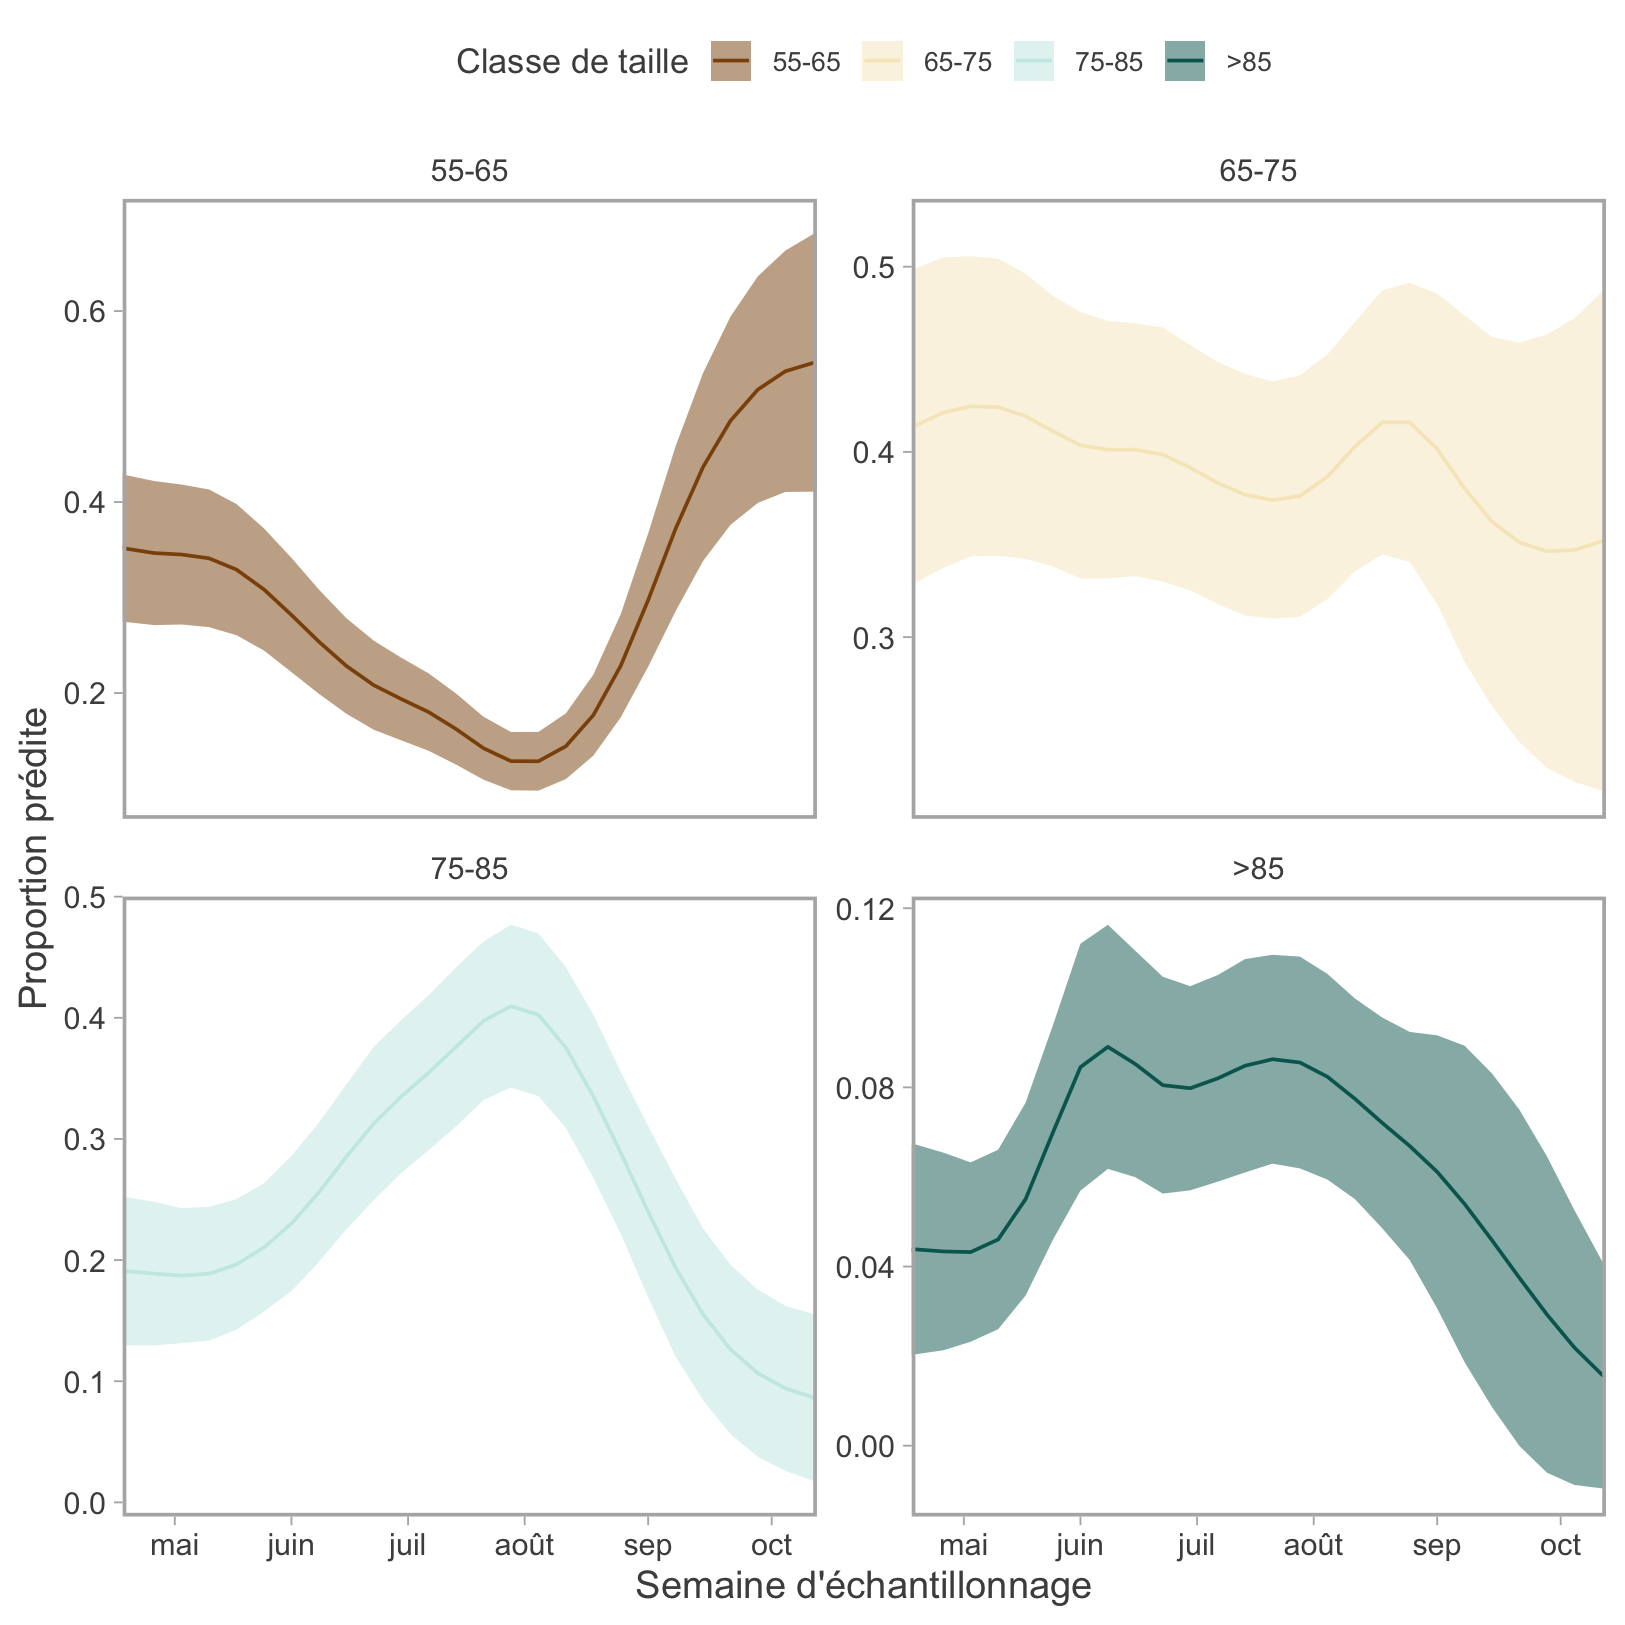
\includegraphics[width=5in]{figs/size_season_preds_chinook.png}}{Figure \ref{fig:season-pred-size}}
    \caption{Composition saisonnière moyenne prédite de la taille basée sur les échantillons de pêche récréative. Le ruban représente l'intervalle de confiance à 95\% de la prédiction moyenne. Les prédictions représentent les effets conditionnels, excluant les termes spatiaux (c.-à-d., représentent l'effet saisonnier « moyen » dans la zone d'étude). Notez que l'échelle de l'axe des y diffère parmi les classes de taille.}
    \label{fig:season-pred-size}
\end{figure}

Les classes de taille du saumon quinnat montraient différentes distributions spatiales entre mai et octobre. La classe de taille 55-65 cm atteignait l'abondance relative maximale près de Victoria et du banc Swiftsure, tandis que l'abondance relative des deux plus grandes classes de taille atteignait un pic près des côtes du banc Swiftsure, ainsi qu'entre Port Renfrew et Sooke. La classe de taille 65-75 cm était plus homogènement distribuée à travers la zone d'étude (Figure \ref{fig:size-spatial-pred-scaled}). La composition de la taille transitait d'être dominée par la classe de taille 65-75 cm au large et sur le banc Swiftsure, vers la classe de taille 75-85 cm près de Port Renfrew, et la plus petite classe de taille au sud de Victoria (Figure \ref{fig:size-spatial-pred}).

\begin{figure}[H]
    \centering
    \pdftooltip{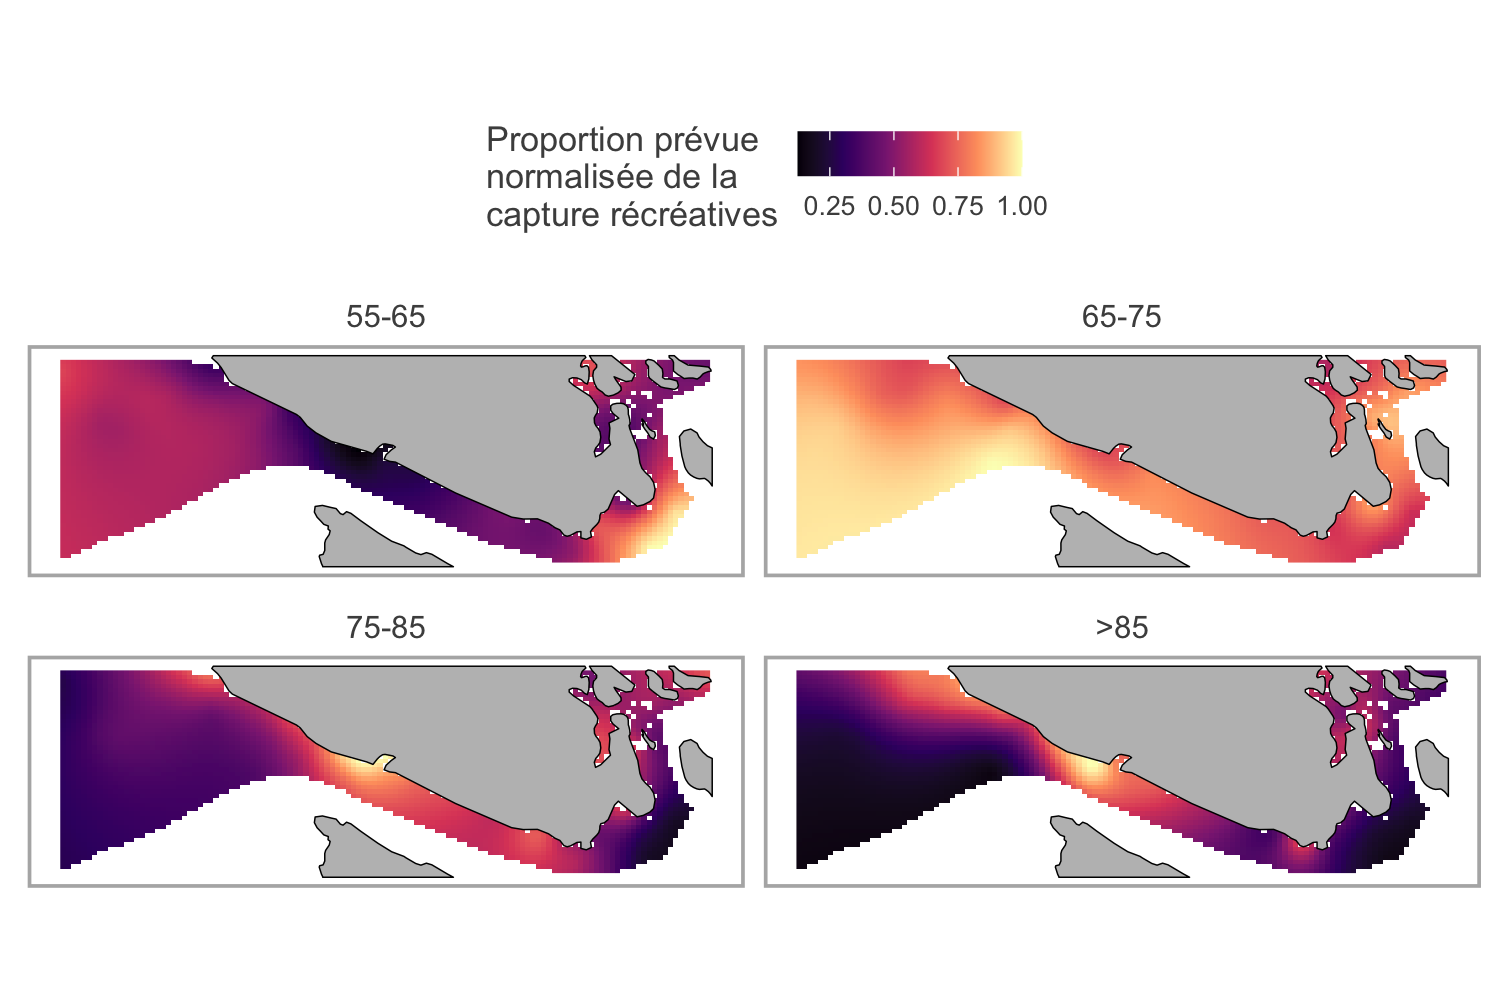
\includegraphics[width=5in]{figs/size_spatial_preds_scaled.png}}{Figure \ref{fig:size-spatial-pred-scaled}}
    \caption{Variation spatiale dans la composition moyenne prédite de la taille mise à l'échelle à travers la portion canadienne du détroit Juan de Fuca et le sud du détroit de Georgie basée sur les échantillons de pêche récréative. Les prédictions sont des moyennes spécifiques aux classes de taille pour mai à octobre et ont été mises à l'échelle relativement à la prédiction maximale à l'intérieur d'une classe de taille pour souligner les différences spécifiques à la taille. Une valeur de un (zéro) indique l'emplacement où une classe de taille était à son abondance prédite maximale (minimale).}
    \label{fig:size-spatial-pred-scaled}
\end{figure}

\begin{figure}[H]
    \centering
    \pdftooltip{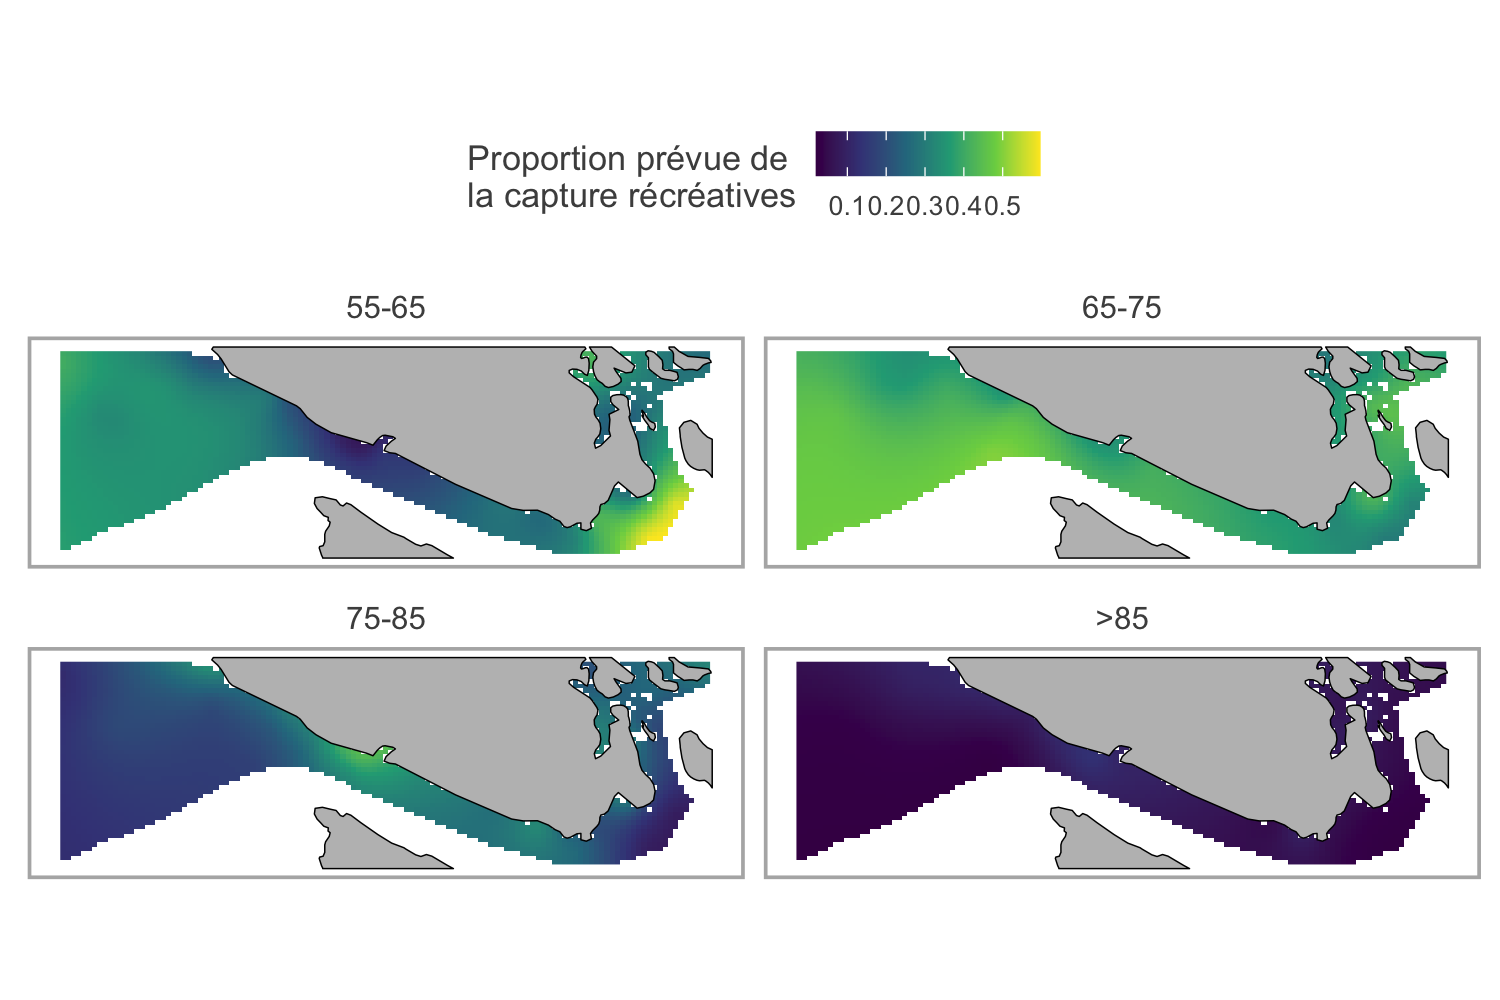
\includegraphics[width=5in]{figs/size_spatial_preds.png}}{Figure \ref{fig:size-spatial-pred}}
    \caption{Variation spatiale dans la composition moyenne prédite de la taille à travers la portion canadienne du détroit Juan de Fuca et le sud du détroit de Georgie basée sur les échantillons de pêche récréative. Les prédictions sont des moyennes spécifiques aux classes de taille pour mai à octobre. Une valeur de un (zéro) indique qu'une classe de taille représentait 100\% (0\%) de l'échantillon moyen prédit.}
    \label{fig:size-spatial-pred}
\end{figure>

Comme pour la composition des stocks, nous avons utilisé un modèle spatio-temporel pour prédire la composition moyenne de la taille à travers l'été pour chaque strate. Le banc Swiftsure et Nitinat avaient des contributions similaires de la plus petite classe de taille, mais Nitinat avait une abondance relativement plus grande des deux plus grandes classes de taille (Figure \ref{fig:stacked-rec}). Port Renfrew avait la contribution relativement la plus grande des grandes classes de taille, avec la proportion moyenne prédite de poissons de plus de 75 cm excédant 65\% en août. Plus à l'est, Sooke/Victoria et les îles Gulf du sud avaient des patrons saisonniers dans la composition de la taille similaires à Nitinat, bien que les poissons plus petits que 55 cm étaient particulièrement abondants à Sooke/Victoria.

\begin{figure}[H]
    \centering
    \pdftooltip{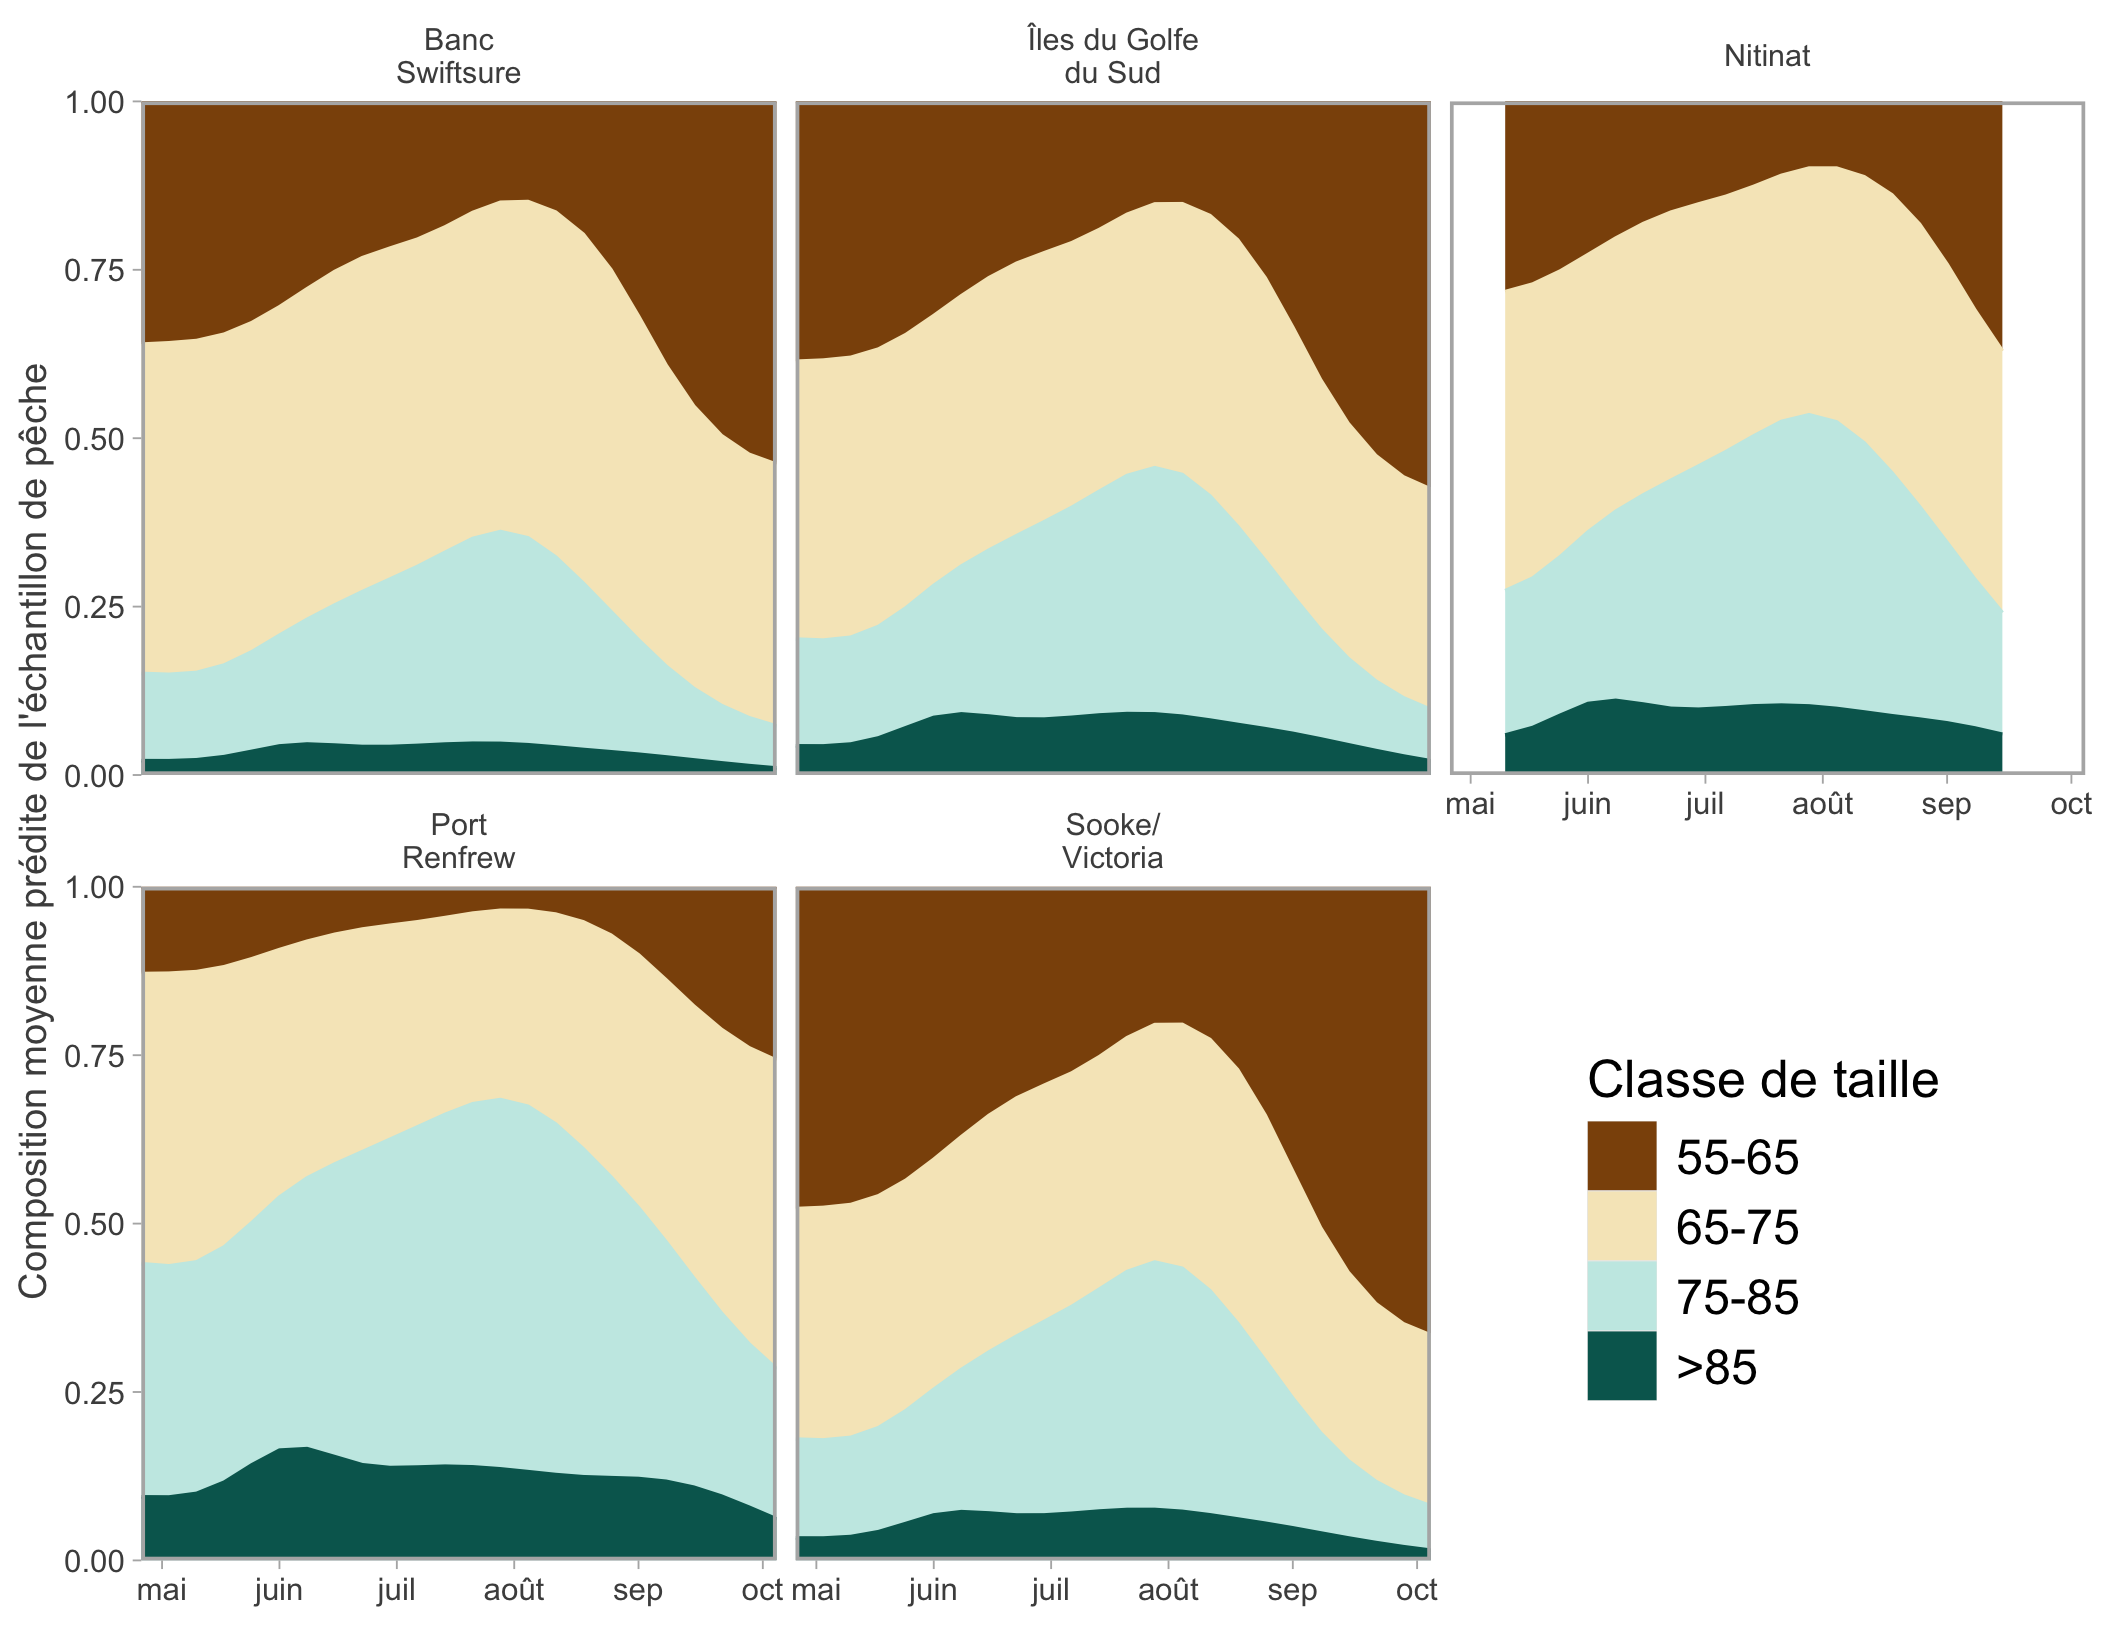
\includegraphics[width=5in]{figs/size_smooth_preds_chinook_stacked.png}}{Figure \ref{fig:stacked-rec-size}}
    \caption{Composition saisonnière moyenne prédite de la taille durant les mois d'été parmi cinq strates spatiales basée sur les échantillons de pêche récréative. Les prédictions ont été estimées en utilisant les emplacements (représentés par un « x ») à l'intérieur de chaque domaine spatial de la Figure \ref{fig:sampling-map} et excluent la variabilité interannuelle. Saanich non montré en raison de données limitées en juillet et août, ainsi que son emplacement à l'extérieur de l'habitat essentiel des ÉRES.}
    \label{fig:stacked-rec-size}
\end{figure}

L'abondance relative de différentes classes de taille variait considérablement parmi les années (Figure \ref{fig:size-smooth-pred-rec-year}). Par exemple, la proportion moyenne prédite de l'échantillon appartenant à la classe de taille supérieure à 85 cm à Port Renfrew en juin variait de 7,7\% à 20,9\% parmi les années d'échantillonnage.

Les résidus du modèle de composition de la taille ajusté étaient appropriément distribués (Figure \ref{fig:qqplot-size}) et les vérifications prédictives postérieures ont confirmé que la composition moyenne simulée des stocks, tenant compte de la variance résiduelle, était généralement similaire à la composition observée de la taille (Figure \ref{fig:posterior-size}). Comme pour le modèle de composition des stocks, les déviations les plus fortes étaient dans les strates avec relativement peu d'échantillons (p. ex., Saanich) ou les classes de taille et strates avec des patrons saisonniers fortement non-linéaires (p. ex., 55-65 cm dans les îles Gulf du sud).

\subsubsection{Contribution des écloseries}

De mai à octobre, le statut d'origine d'écloserie ou sauvage pouvait être déterminé pour la plupart des échantillons de la pêche récréative. Les individus d'origine d'écloserie étaient relativement communs dans toutes les strates, mais constituaient la majorité de la capture dans la plupart des mois dans les strates du banc Swiftsure, Nitinat, et Saanich (Figure \ref{fig:bar-hatchery-summer}). Inversement, les poissons d'origine sauvage étaient relativement plus abondants, particulièrement en août, dans les strates Port Renfrew et Sooke/Victoria (Figure \ref{fig:bar-hatchery-summer}).

\begin{figure}[H]
    \centering
    \pdftooltip{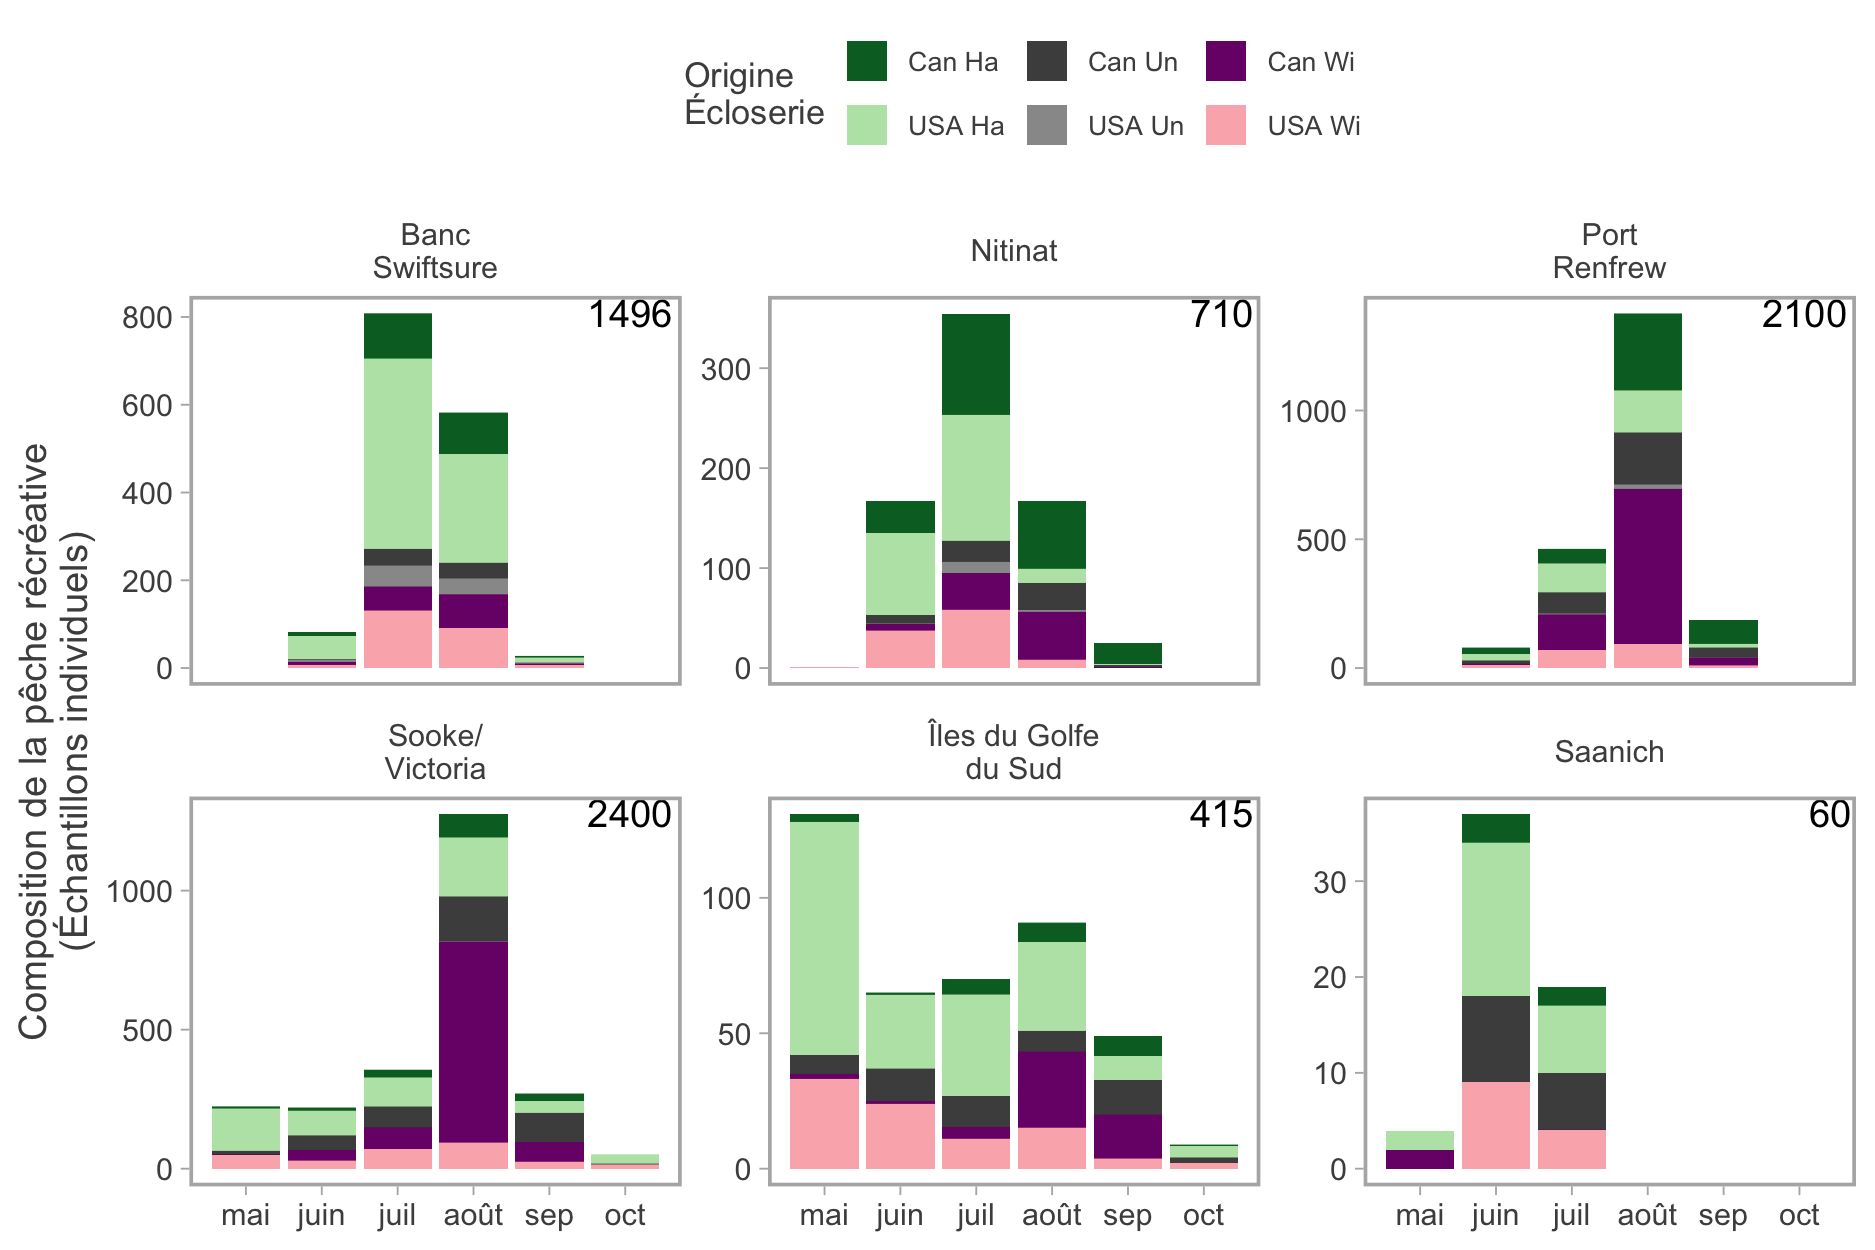
\includegraphics[width=5in]{figs/rec_monthly_hatchery_comp_bar_summer.png}}{Figure \ref{fig:bar-hatchery-summer}}
    \caption{Abondance relative d'individus d'origine d'écloserie (vert), sauvage (violet), et inconnue (gris), groupés par pays (Canada foncé; États-Unis pâle). Les assignations inconnues se sont produites quand un individu avec une nageoire adipeuse intacte était assigné, basé sur l'ISG, à un stock sans marquage de masse et couverture de marquage basé sur la parenté incomplète.}
    \label{fig:bar-hatchery-summer}
\end{figure}

Les stocks différaient dans la contribution relative d'individus d'origine d'écloserie, sauvage et inconnue. La majorité des individus des stocks américains étaient d'origine d'écloserie (approximativement 55-75\%) et relativement peu étaient non assignés en raison de la prévalence du marquage de masse dans les écloseries de Washington et de l'Oregon (Figure \ref{fig:bar-hatchery-stocks}). La contribution de poissons d'écloserie aux stocks canadiens était plus variable et il y avait une plus grande proportion d'individus d'origine inconnue due au fait que peu d'écloseries canadiennes emploient le marquage de masse. Bien que la couverture TPB soit actuellement répandue dans les écloseries canadiennes, la couverture a varié à travers le temps et était faible avant l'année de ponte 2013 (Figure \ref{fig:pbt-coverage}). Ainsi plusieurs poissons, particulièrement ceux capturés avant approximativement 2017, ne pouvaient pas être assignés un statut d'écloserie de manière fiable.

\begin{figure}[H]
    \centering
    \pdftooltip{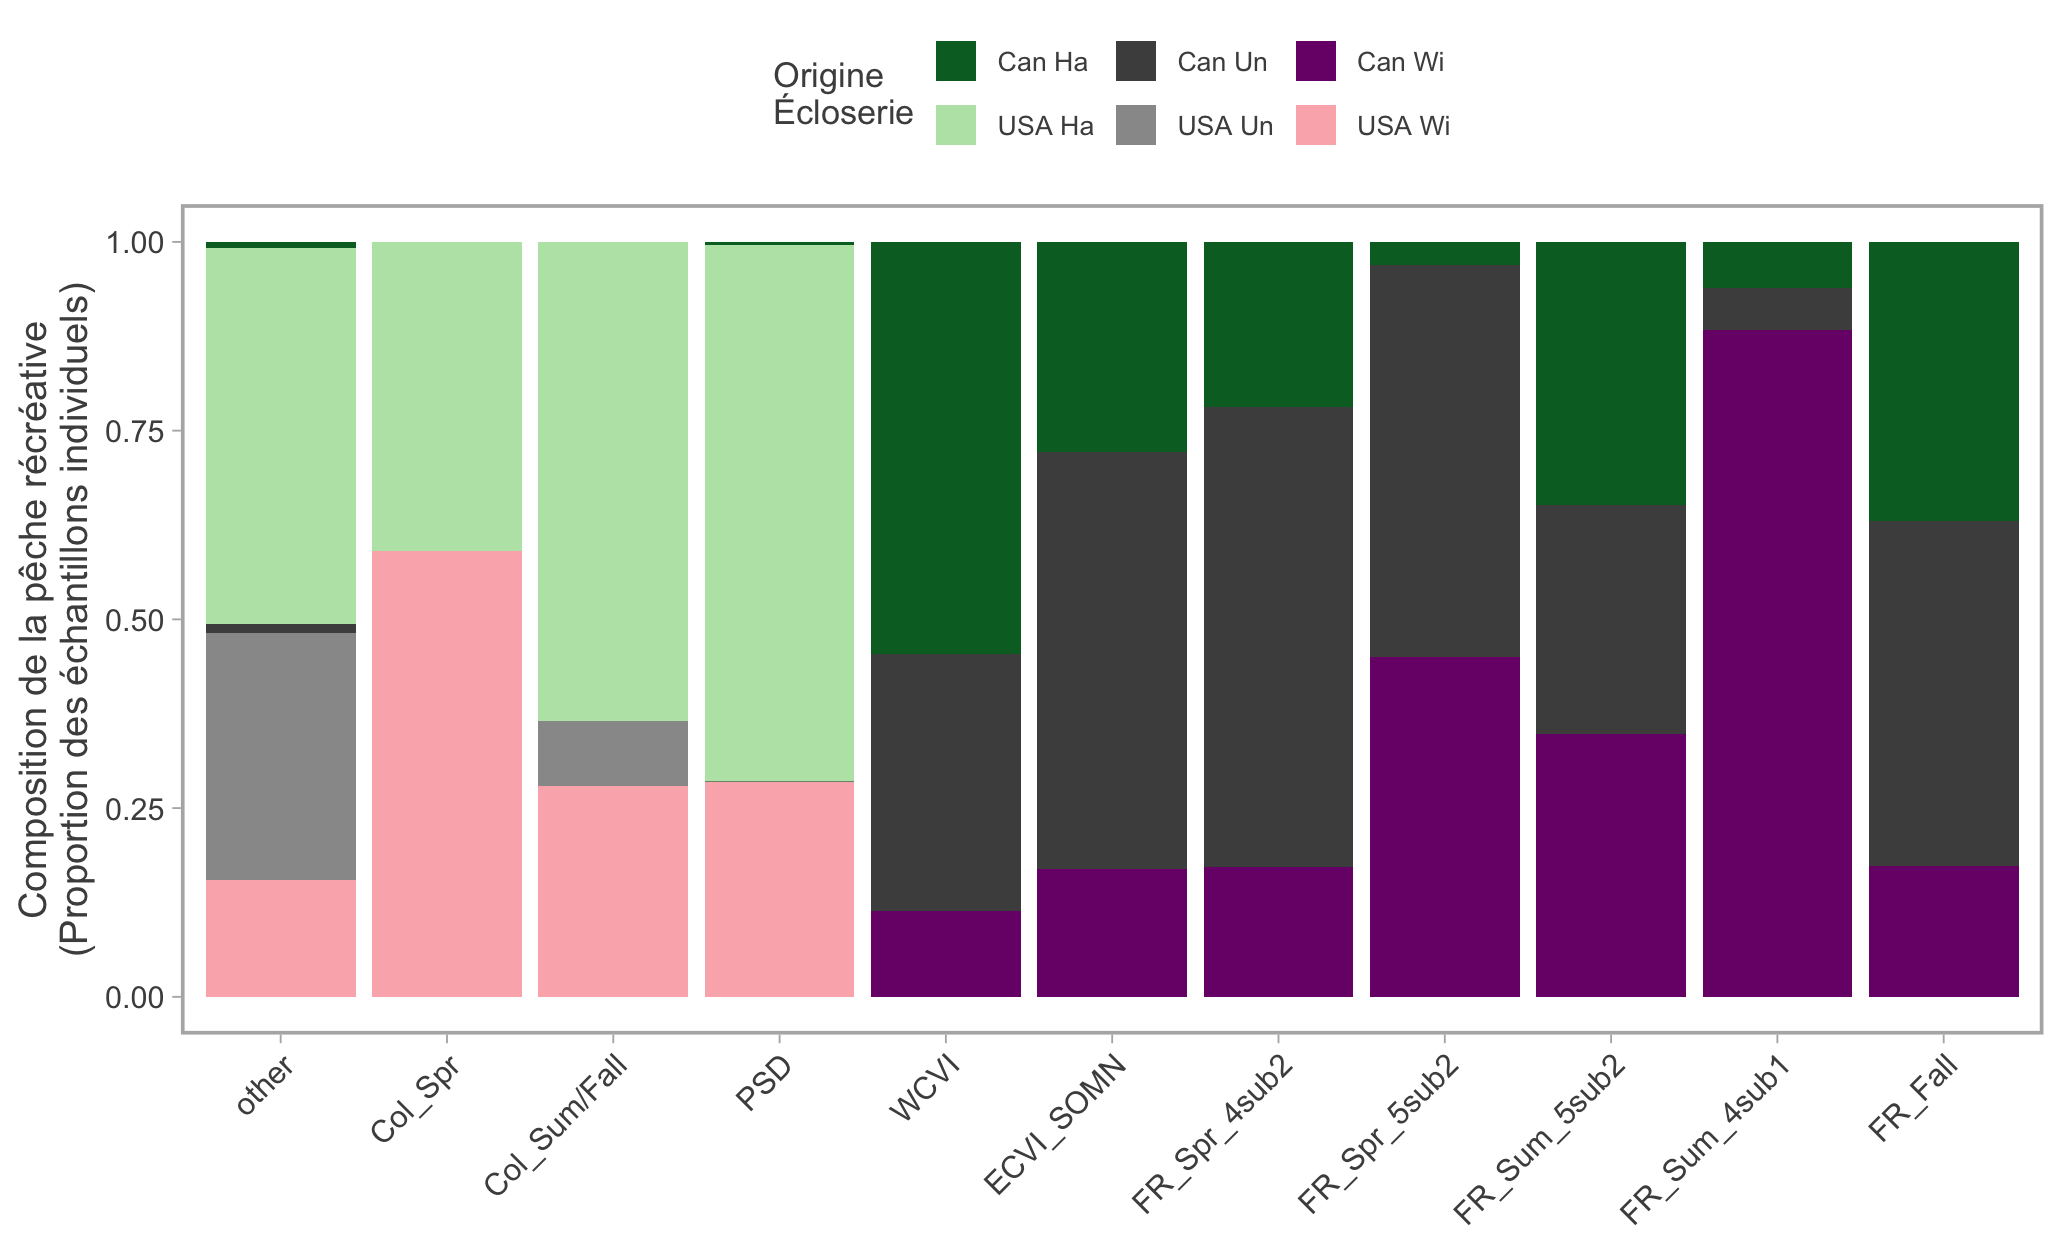
\includegraphics[width=5in]{figs/rec_stock_hatchery_bar.png}}{Figure \ref{fig:bar-hatchery-stocks}}
    \caption{Abondance relative d'individus d'origine d'écloserie (vert), sauvage (violet), et inconnue (gris) dans chaque stock. Les assignations inconnues se sont produites quand un individu avec une nageoire adipeuse intacte était assigné à un stock sans marquage de masse ou couverture de marquage basé sur la parenté incomplète.}
    \label{fig:bar-hatchery-stocks}
\end{figure}

La proportion de géniteurs d'origine d'écloserie (pHOS) entre 2014 et 2022 différait parmi les stocks canadiens et parmi les années (Figure \ref{fig:box-phos}). Le pHOS moyen était de 72\% parmi les populations surveillées dans le stock COIV et de 53\% pour les populations à l'intérieur du stock COIV/SOMN. Les niveaux pHOS étaient légèrement plus bas parmi les stocks de la rivière Fraser, mais la plupart des stocks avaient seulement une ou deux populations améliorées par écloserie (Figure \ref{fig:box-phos}). Il y avait une variabilité considérable parmi les populations à l'intérieur d'un stock, soulignant que les estimations au niveau des stocks des contributions d'écloserie basées sur le pHOS seul devraient être interprétées avec prudence.

\subsection{Sélectivité dans les restes de proies des ÉRES}

Nous avons utilisé des simulations Monte Carlo pour tester l'évidence que la composition observée des stocks et de la taille des restes de proies des ÉRES (collectés après 2016 et dans les strates du banc Swiftsure, Nitinat, et Port Renfrew) déviait de la composition attendue telle qu'indexée par la pêche récréative. Notre approche tenait compte de la variabilité spatiale, saisonnière, et interannuelle en utilisant les modèles de composition décrits précédemment, tout en propageant l'incertitude due à l'assignation génétique des stocks, l'assignation de l'âge, les petites tailles d'échantillon, et les paramètres estimés du modèle.

Nous avons trouvé de l'évidence de sélection positive pour les stocks Fraser rivière printemps $5.2$, été $5.2$, et été $4.1$ (Figure \ref{fig:sel-stock}). Ces stocks constituaient 4-36\% de plus de l'échantillon observé de restes de proies que prédit par le modèle de composition des stocks paramétrisé avec les données de pêche récréative. Inversement, les stocks COIV, Puget Sound, Columbia été/automne, et « Autre » étaient sous-représentés dans les restes de proies, avec leur contribution proportionnelle 5-27\% de moins que la prédiction du modèle (Figure \ref{fig:sel-stock}). Il n'y avait pas d'évidence de sélectivité dans les stocks restants, probablement parce que leur abondance relative observée était faible dans les restes de proies et prédite pour être faible aux moments et emplacements où les restes de proies ont été collectés (Figures \ref{fig:bar-diet}, \ref{fig:stacked-rec}).

\begin{figure}[H]
    \centering
    \pdftooltip{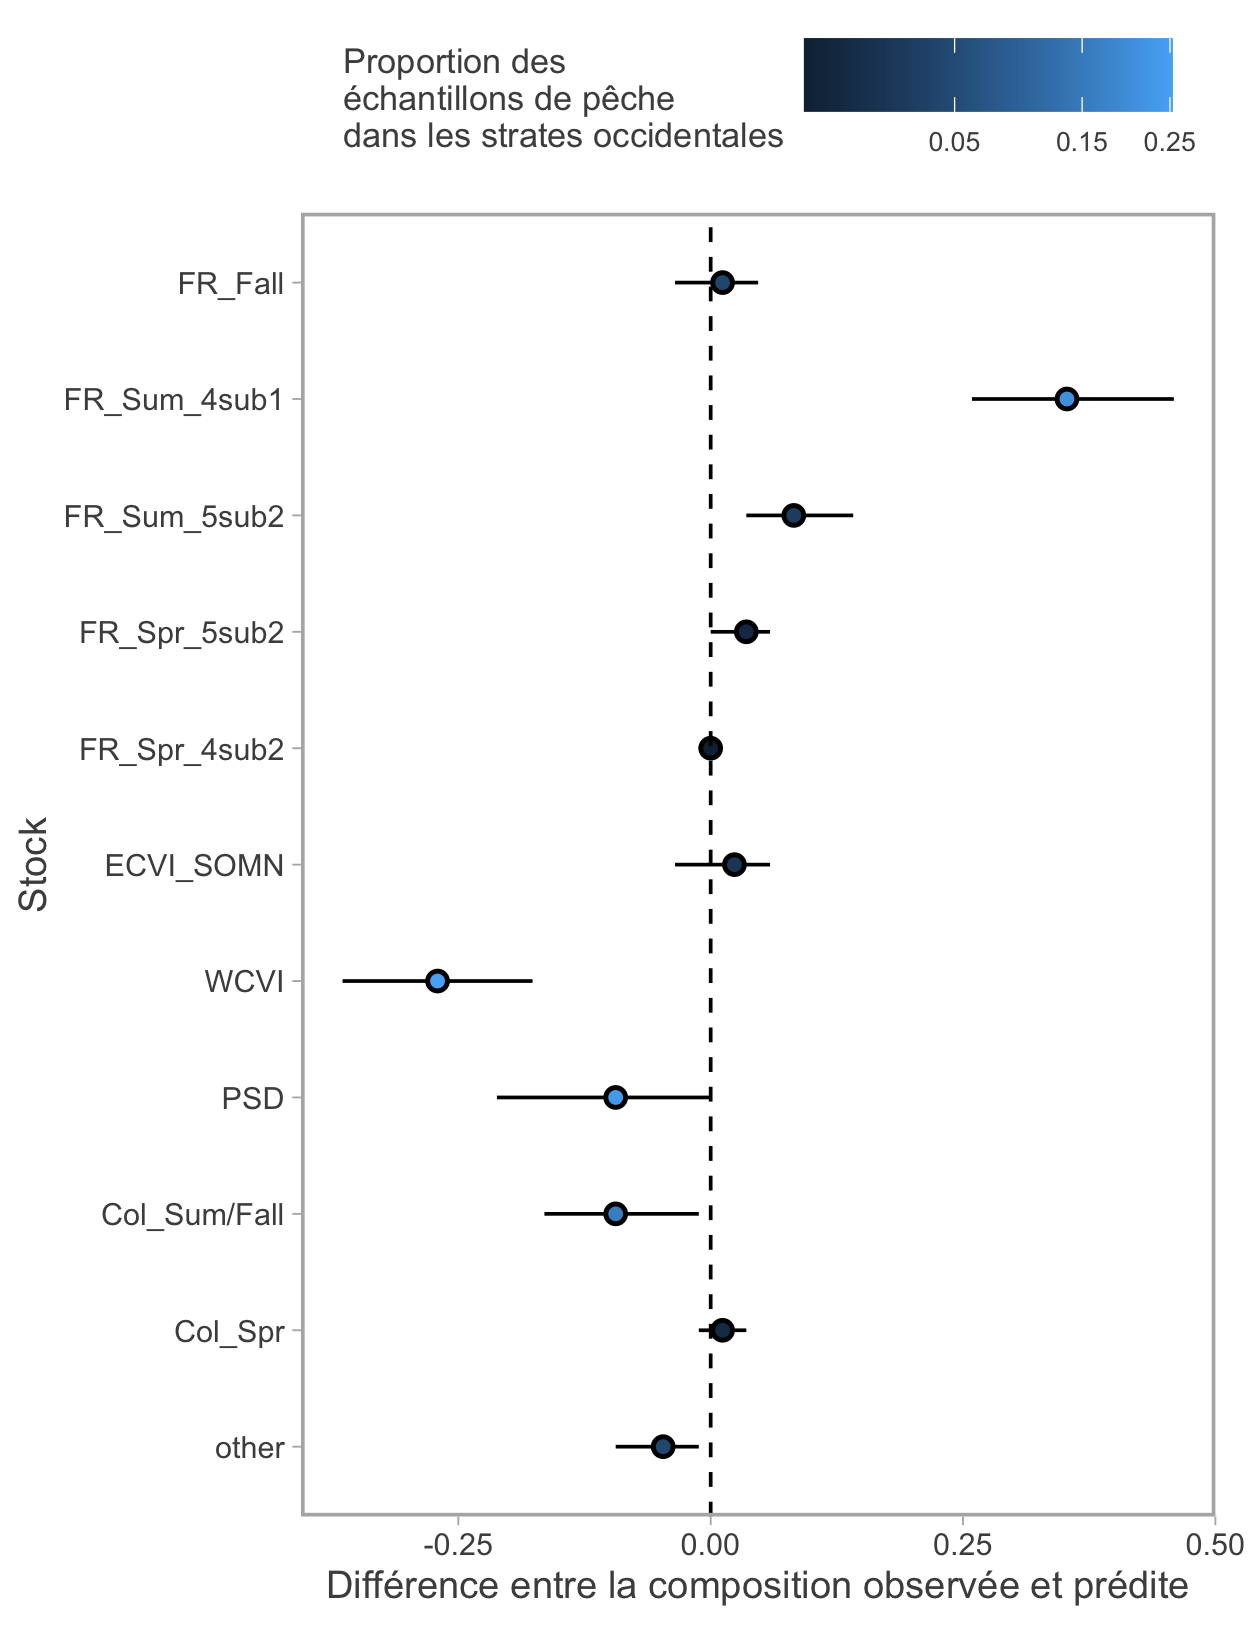
\includegraphics[width=5in]{figs/selectivity_bean_stock.png}}{Figure \ref{fig:sel-stock}}
    \caption{Différences entre la contribution observée et prédite par le modèle de chaque stock aux restes de proies des ÉRES. Les valeurs positives (négatives) indiquent qu'un stock donné était observé plus (moins) fréquemment dans les restes de proies des ÉRES que prédit par le modèle dépendant de la pêche. Les points représentent les médianes et les moustaches représentent les intervalles du 95e percentile parmi 500 simulations Monte Carlo. Les points plus brillants (plus foncés) représentent les stocks qui étaient plus (moins) communs dans les échantillons de pêche récréative des moments et strates coïncidents avec les restes de proies des ÉRES.}
    \label{fig:sel-stock}
\end{figure}

Les deux plus petites classes de taille du saumon quinnat constituaient une proportion plus petite (approximativement 10\% et 7\% respectivement) des restes de proies observés que prédit par le modèle de composition de la taille paramétrisé avec les données de pêche récréative (Figure \ref{fig:sel-size}). Nous avons aussi trouvé de l'évidence de sélection positive pour les deux plus grandes classes de taille, qui étaient approximativement 8\% plus communes dans les restes de proies observés que prédit par le modèle (Figure \ref{fig:sel-size}). Les estimations de sélectivité pour les deux classes de taille intermédiaires (65-75 et 75-85 cm) étaient plus incertaines que les deux autres classes de taille malgré des médianes similaires (Figure \ref{fig:sel-size}).

\begin{figure}[H]
    \centering
    \pdftooltip{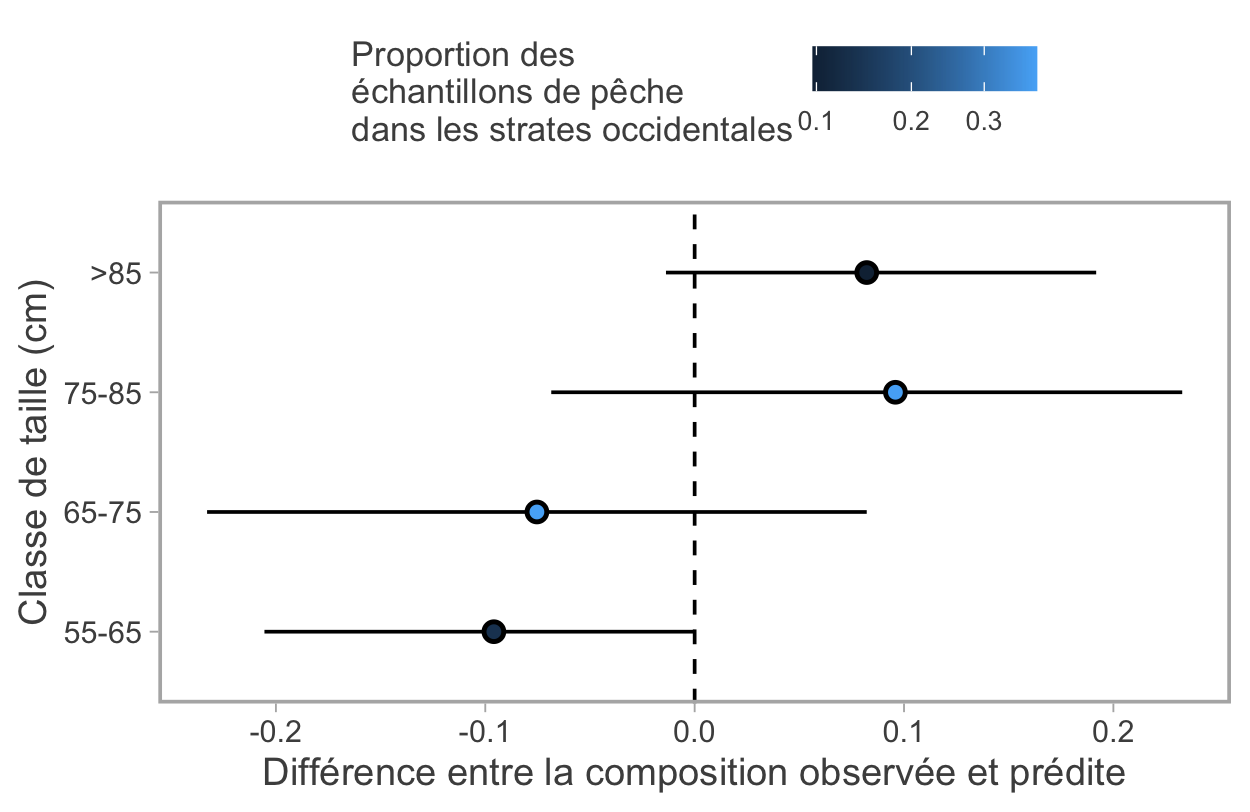
\includegraphics[width=5in]{figs/selectivity_bean_size.png}}{Figure \ref{fig:sel-size}}
    \caption{Différences entre la contribution observée et prédite par le modèle de chaque classe de taille aux restes de proies des ÉRES. Les valeurs positives (négatives) indiquent qu'une classe de taille donnée était observée plus (moins) fréquemment dans les restes de proies des ÉRES que prédit par le modèle dépendant de la pêche. Les points représentent les médianes et les moustaches représentent les intervalles du 95e percentile parmi 500 simulations Monte Carlo. Les points plus brillants (plus foncés) représentent les classes de taille qui étaient plus (moins) communes dans les échantillons de pêche récréative des moments et strates coïncidents avec les restes de proies des ÉRES.}
    \label{fig:sel-size}
\end{figure>

\subsection{Analyses de sensibilité}

Le modèle de composition des stocks qui a été ajusté aux données qui incluaient seulement les échantillons de pêches récréatives supérieurs à 75 cm de longueur à la fourche a prédit une composition des stocks légèrement différente, particulièrement tôt dans l'année (Figures \ref{fig:comb-pred-stock1}, \ref{fig:comb-pred-stock2}). Cependant, les mêmes stocks montraient de l'évidence de sélectivité positive et négative (Figure \ref{fig:comb-sel-stock}). Similairement, les résultats de sélectivité des stocks et de sélectivité de la taille étaient similaires quand les échantillons qui chevauchaient avec les interventions de gestion des pêches étaient exclus. Détails additionnels dans l'Annexe \ref{sensitivity}.

\subsection{Abondance terminale du saumon quinnat}

Tous les stocks de saumon quinnat présents dans la zone d'étude ont montré des tendances cycliques dans l'abondance terminale au cours des 40 dernières années; cependant, ces dynamiques n'ont pas été homogènes. Les stocks côtiers de Washington et de l'Oregon (inclus dans le stock « Autre » à travers cette analyse); Columbia rivière printemps; et Fraser rivière printemps $4_2$, printemps $5_2$, et été $5_2$ ont décliné à travers les années 2010 et ont montré des degrés variables de récupération (Figure \ref{fig:esc-stock}). Inversement, l'abondance terminale des stocks COIV, COIV/SOMN, et Fraser rivière été $4_1$ a augmenté (Figure \ref{fig:esc-stock}).

\begin{figure}[H]
    \centering
    \pdftooltip{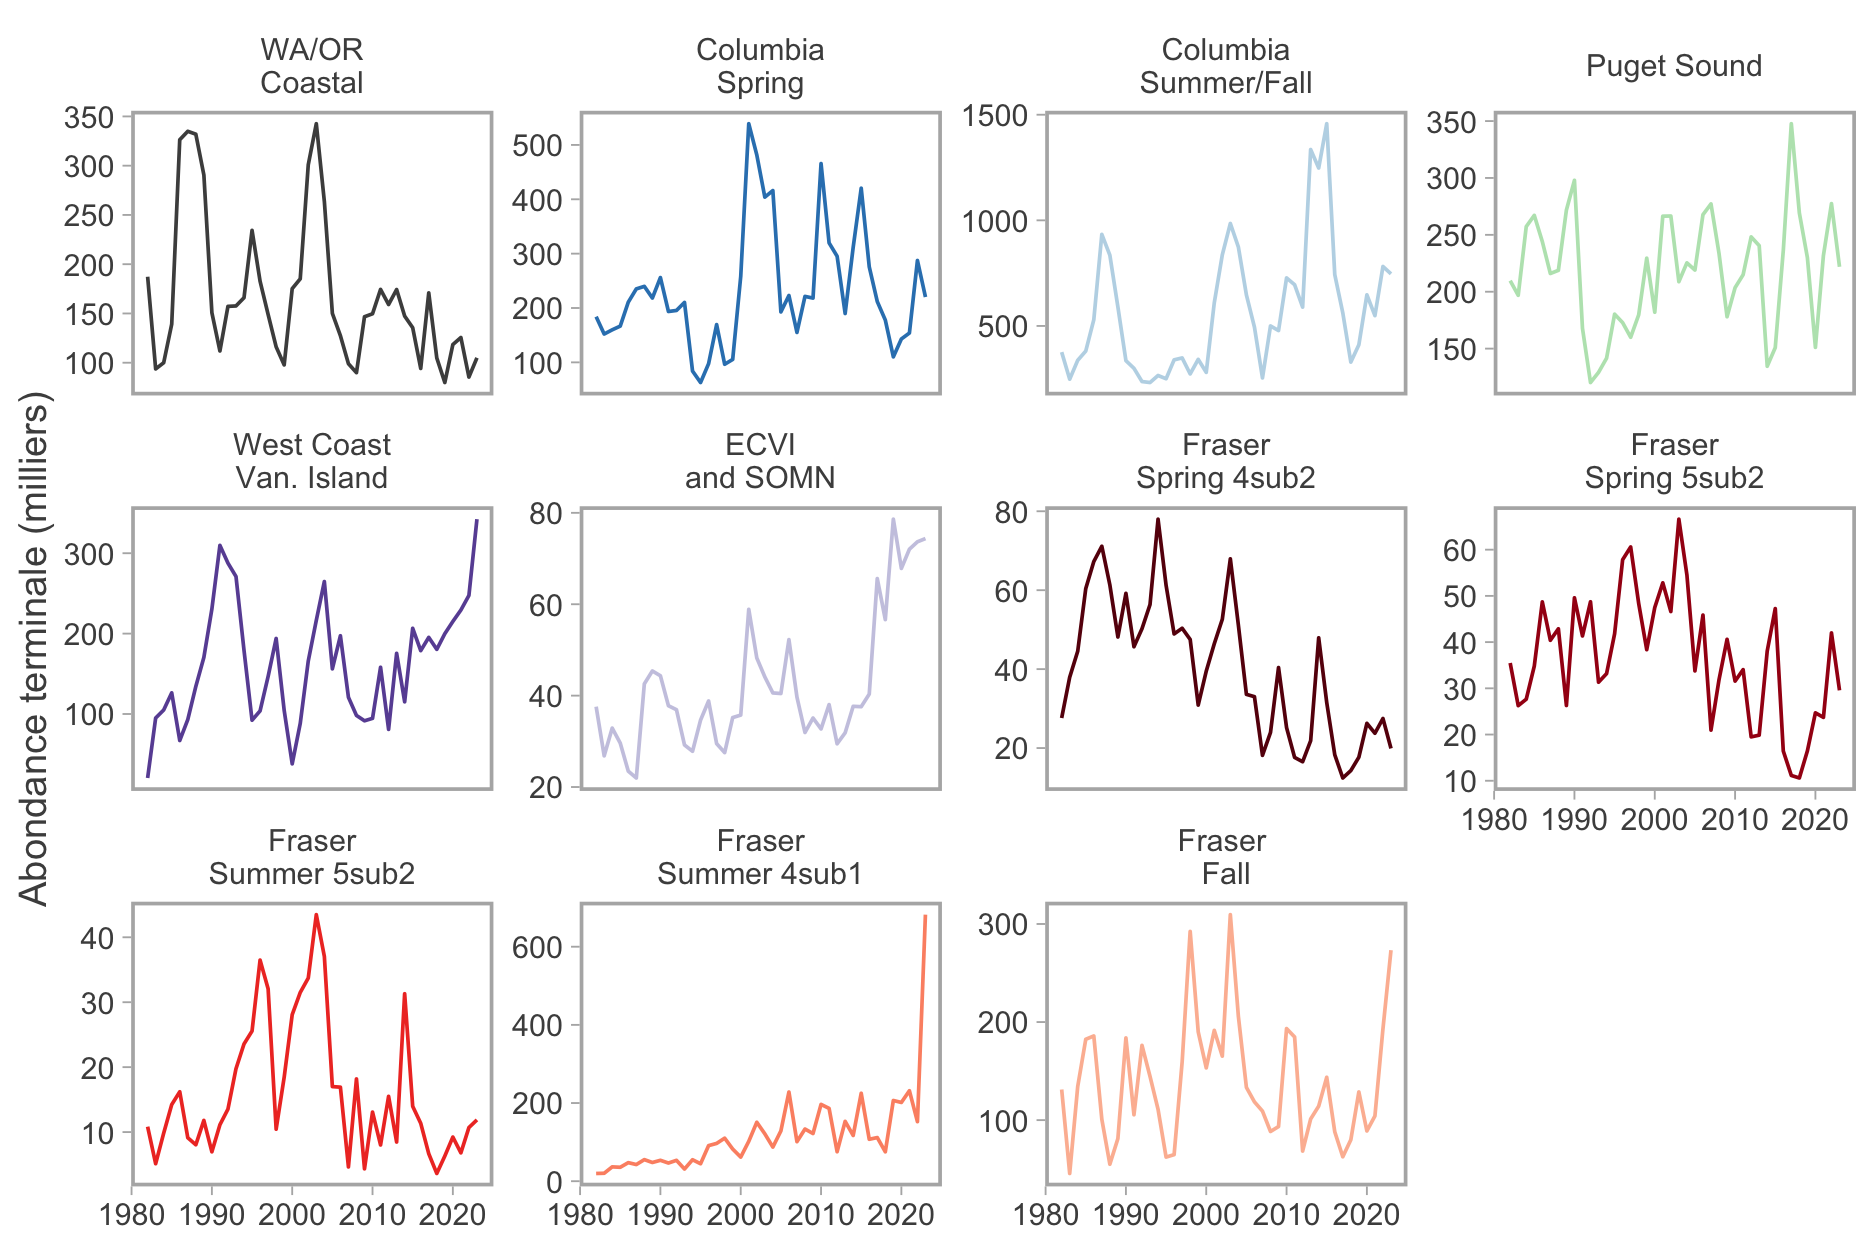
\includegraphics[width=5in]{figs/escapement_stock_group.png}}{Figure \ref{fig:esc-stock}}
    \caption{Abondance terminale des stocks de saumon quinnat. Les populations côtières de Washington et de l'Oregon (WA/OR) sont incluses dans le stock « Autre » à travers ce manuscrit. Les données de 2023 n'étaient pas disponibles pour les stocks côtiers WA/OR et Puget Sound et ont été imputées basées sur les moyennes 2019-2022. Les échelles de l'axe des Y diffèrent parmi les stocks. Définitions de l'abondance terminale et sources de données disponibles dans l'Annexe \ref{terminal-abundance}.}
    \label{fig:esc-stock}
\end{figure}

L'abondance terminale agrégée (c.-à-d., sommée parmi les stocks) a aussi varié cycliquement, mais est relativement élevée comparée à l'abondance terminale avant 2000 (Figure \ref{fig:esc-stock}). Généralement la majorité de l'abondance terminale agrégée provient des stocks de la côte extérieure (côtiers de Washington et de l'Oregon, Columbia rivière, côte ouest de l'île de Vancouver); cependant, la contribution des stocks qui frayent dans les bassins versants de la mer des Salish a augmenté durant les années récentes.

\begin{figure}[H]
    \centering
    \pdftooltip{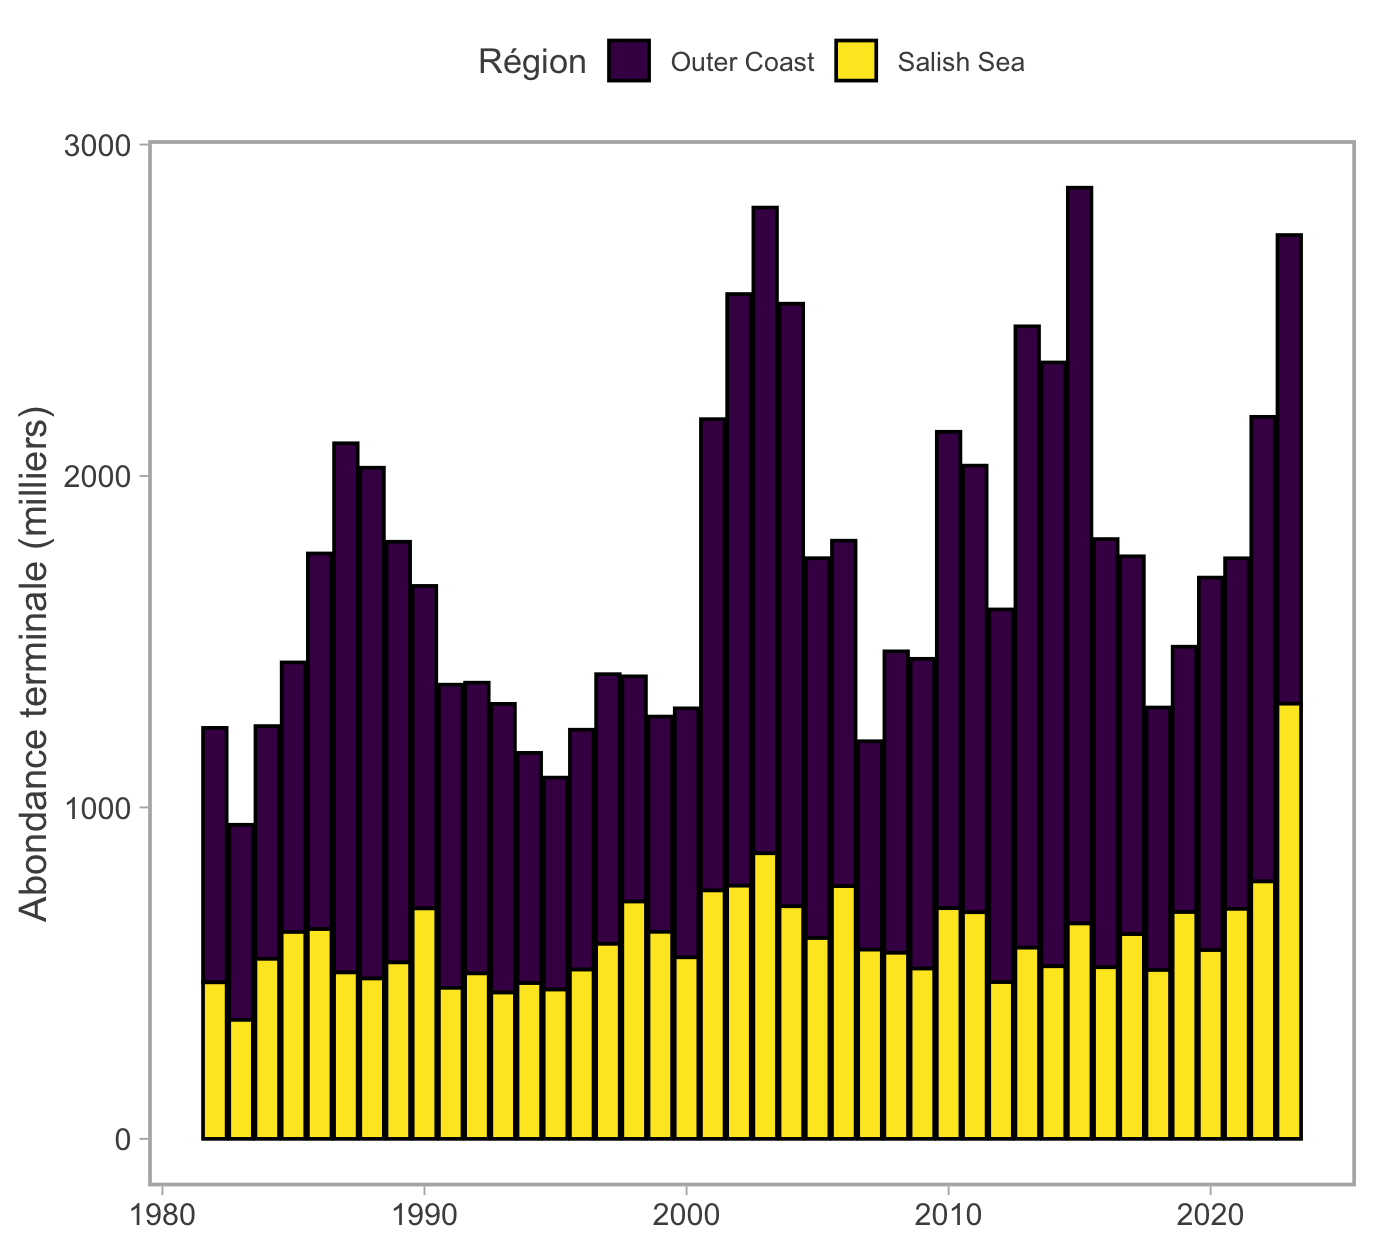
\includegraphics[width=5in]{figs/escapement_region.png}}{Figure \ref{fig:esc-region}}
    \caption{Abondance terminale agrégée des stocks de saumon quinnat, communs dans l'habitat essentiel des ÉRES, frayant à l'intérieur de la mer des Salish (jaune) ou dans la côte extérieure, incluant la Columbia rivière (violet). Les barres légèrement ombrées représentent les valeurs moyennes sur cinq ans. 2023 n'est pas montré étant donné les données manquantes pour les stocks côtiers de Washington et Puget Sound. Définitions de l'abondance terminale et sources de données disponibles dans l'Annexe \ref{terminal-abundance}.}
    \label{fig:esc-region}
\end{figure}

\section{DISCUSSION}\label{sec:discussion}

Notre compréhension de la relation entre les ÉRES et le saumon quinnat a évolué au cours des cinq dernières décennies. Depuis l'identification de l'écotype « résident » se nourrissant de poissons \citep{fordSelectiveForagingFisheating2006} jusqu'à la corrélation entre les indices d'abondance du saumon quinnat à l'échelle de la côte et la mortalité des épaulards résidents \citep{fordChinookSalmonPredation2010}, l'importance du saumon quinnat comme proie principale est incontestée. Cependant, la variabilité de l'abondance et de la distribution saisonnière des stocks contribuant aux indices de saumon quinnat à l'échelle de la côte, ainsi que l'influence probable d'autres menaces, ont obscurci la relation entre l'abondance du quinnat et la dynamique des populations d'ÉRES \citep{velez-espinoRelativeImportanceChinook2015, nelsonIdentifyingDriversDemographic2024, saygiliPrevalenceChinookSalmon2024}.

Dans cette étude, nous avons exploité des échantillons de restes de proies d'ÉRES et de pêches récréatives, tous deux collectés dans l'habitat essentiel des ÉRES dans le sud de la Colombie-Britannique, pour explorer trois questions interconnectées. Premièrement, quels stocks de saumon quinnat et quelles classes de taille sont les plus couramment observés dans l'alimentation des ÉRES ? Deuxièmement, quelle est la composition du champ de proies disponible pour les ÉRES, particulièrement dans les endroits où les données sur les restes de proies sont limitées ? Troisièmement, y a-t-il des preuves de butinage sélectif par stock ou par taille chez les ÉRES ? Nous présentons nos résultats dans le contexte plus large des changements dans l'abondance du saumon quinnat, de la variabilité du supplément de pisciculture entre les stocks, et des facteurs potentiels de sélectivité par les ÉRES. Enfin, nous relions nos résultats aux actions de gestion potentielles qui pourraient améliorer la disponibilité du saumon quinnat pour les ÉRES. Reconnaître les différences entre les régimes alimentaires observés et le champ de proies disponible fournit un degré de granularité nécessaire pour envisager les opportunités d'options de gestion raffinées à l'appui des besoins en proies des ÉRES.

\subsection{Composition des restes de proies des ÉRES}

Les échantillons de restes de proies d'ÉRES collectés pendant les mois d'été entre le détroit Juan de Fuca et les îles San Juan étaient dominés par un sous-ensemble de stocks de saumon quinnat du fleuve Fraser. Les poissons Fraser Spring $5_2$ et Summer $5_2$, des stocks avec un cycle vital de saumoneau d'un an et une période de montaison précoce, étaient relativement abondants en juin et juillet, tandis que les individus Fraser Summer $4_1$ de saumoneau de l'année constituaient la composante dominante dans l'ensemble, particulièrement en juillet et août. Les stocks restants ont été observés à une abondance relativement faible. Il y avait des preuves que les stocks précoces de saumoneaux d'un an constituaient une proportion plus petite du régime alimentaire dans la période actuelle que dans la période précoce ; cependant, nous n'avons pas pu tester cette hypothèse en raison des différences dans le moment et l'emplacement de l'échantillonnage. Bien que nous n'ayons pas pu identifier de manière fiable le saumon quinnat d'origine de pisciculture dans les restes de proies d'ÉRES, sept échantillons ont été identifiés sur la base de l'ITGP et provenaient de piscicultures du bas Fraser Fall, COIV, et COIV.

Nous avons également évalué la composition de taille des régimes alimentaires des ÉRES, en utilisant les écailles pour estimer la longueur à la fourche moyenne des restes de proies échantillonnés basée sur les relations taille-âge. Le saumon quinnat prédit comme étant plus petit que 65 cm de longueur à la fourche était largement absent des échantillons identifiés par âge, qui étaient plutôt dominés par les classes de taille de 75-85 et >85 cm. Ces tendances sont cohérentes avec les observations estivales antérieures de la mer des Salish qui ont trouvé que les populations intérieures du fleuve Fraser et les classes d'âge plus anciennes étaient des composantes majeures des régimes alimentaires des ÉRES \citep{fordSelectiveForagingFisheating2006, hansonSpeciesStockIdentification2010}.

Trop peu d'échantillons de restes de proies ont été collectés pour tenir compte statistiquement de la variabilité entre les périodes d'échantillonnage, les semaines d'échantillonnage et les emplacements spatiaux. Bien que les observations d'emplacements et de mois avec un plus grand nombre d'échantillons soient plus fiables que celles avec moins, sans modèle nous ne pouvons pas présenter d'estimations d'incertitude fiables ou déterminer la taille d'échantillon minimale nécessaire pour tirer des inférences de manière fiable \citep[p. ex.,][]{tritesDietaryAnalysisFecal2005}. Nous mettons en garde contre l'hypothèse que les régimes alimentaires des ÉRES dans des endroits ou des mois sans échantillons seront similaires aux observations ailleurs, étant donnée la variabilité saisonnière et spatiale dans la composition des stocks et des tailles de saumon quinnat.

\subsection{Composition de la pêche récréative}

Les stocks de saumon quinnat diffèrent dans leur distribution, leurs caractéristiques physiques et leur moment de migration en eau douce \citep{healeyLifeHistoryChinook1991, weitkampMarineDistributionsChinook2010}, résultant en une variabilité spatiale et saisonnière substantielle dans l'abondance spécifique aux stocks dans les habitats marins \citep{sheltonUsingHierarchicalModels2019, freshwaterIntegratedModelSeasonal2021}. Nous avons exploité un grand nombre d'échantillons collectés dans les pêches récréatives canadiennes pour quantifier la variabilité dans la composition des stocks et des tailles de saumon quinnat à des échelles particulièrement fines. Nous avons trouvé des différences marquées dans la composition de la pêche récréative entre les semaines d'échantillonnage à l'intérieur d'un endroit et entre des endroits distants de cinq à dix kilomètres à l'intérieur d'une semaine d'échantillonnage.

Un facteur principal de variation temporelle dans la composition des stocks de saumon quinnat est la contribution relative des stocks résidents, qui sont présents dans les habitats du plateau continental méridional toute l'année, et des stocks migrateurs qui deviennent plus abondants à mesure que les individus matures migrent vers les habitats d'eau douce. Par exemple, le stock de Puget Sound est présent dans la mer des Salish toute l'année \citep{oneillMarineDistributionLife2009, freshwaterIntegratedModelSeasonal2021}, et dominait la composition des pêches récréatives, particulièrement tôt en été. Inversement, les stocks du fleuve Fraser, à l'exception des individus de montaison automnale, migrent typiquement vers le nord le long du plateau continental ou au large \citep{ctc2021AnnualReport2022}. La composition des stocks montrait des pics successifs alors que les reproducteurs de retour Spring $4_2$, puis Spring $5_2$, Summer $5_2$, et Summer $4_1$ migraient vers le fleuve Fraser. Les individus COIV, qui atteignent typiquement la maturité dans les eaux de l'Alaska \citep{sheltonUsingHierarchicalModels2019}, et les individus Fraser River Fall, qui sont résidents le long du plateau et dans le nord du détroit de Georgie, étaient abondants dans des endroits spécifiques à la fin de l'été. Notamment, les individus Columbia River Spring étaient rares, même dans les zones extérieures, suggérant que ce stock peut migrer plus au large jusqu'à atteindre le fleuve Columbia.

Les tendances spatiales différaient également entre les stocks. Les individus COIV étaient largement contraints aux eaux côtières du lac Nitinat à Port Renfrew. Les individus Columbia River Summer/Fall étaient abondants du banc Swiftsure vers l'ouest jusqu'au banc La Perouse. Cette région incluait également une contribution relativement importante de poissons Fraser River Fall, cohérente avec les données récentes de prises accessoires au chalut \citep{lagasseReviewSalmonBycatch2024}, et indiquant qu'elle pourrait être une zone d'élevage pour ce stock. Les individus Fraser River Summer $4_1$ étaient les plus abondants dans le détroit Juan de Fuca. Enfin, les individus de Puget Sound étaient répandus du Swiftsure à l'est jusqu'au sud du détroit de Georgie, mais étaient plus dominants dans les zones côtières.

Les différences dans la composition des tailles sont associées à la composition des stocks parce que le saumon quinnat varie en taille et âge à maturité \citep{healeyLifeHistoryChinook1991}, mais elles reflètent également des différences ontogénétiques alors que les poissons continuent de grandir pendant l'été et montrent des changements dans l'utilisation de l'habitat \citep{freshwaterChinookSalmonDepth2024, freshwaterSeasonalVariabilityCondition2024}. Généralement, les poissons plus petits que 65 cm étaient les plus abondants tôt et tard dans l'année, avant et après que les individus reproducteurs aient migré à travers la zone. Les classes de taille 75-85 et >85 cm montraient la tendance opposée, tandis que la classe de taille 65-75 cm montrait une faible variabilité saisonnière. Les deux classes de taille plus grandes sont principalement des poissons matures, mais cette dernière inclut à la fois des poissons sexuellement matures, ainsi que des individus qui resteront en mer pour une année supplémentaire \citep{freshwaterChinookSalmonDepth2024, freshwaterSeasonalVariabilityCondition2024}. Les tendances spatiales soutenaient également cette hypothèse---les poissons plus petits que 75 cm étaient répandus et particulièrement abondants au large du banc Swiftsure et au sud de Victoria, des endroits communément considérés comme habitat d'élevage pour les poissons résidents, tandis que ceux plus grands que 75 cm étaient concentrés près de l'embouchure du détroit Juan de Fuca. Les points chauds d'abondance pour les classes de taille plus grandes étaient similaires aux endroits où les comportements de recherche de nourriture des ÉRES sont le plus couramment observés \citep{thorntonSouthernResidentKiller2022}.

Les estimations de composition des stocks et des tailles ont le potentiel d'être fortement influencées par les mesures de gestion telles que les pêches sélectives par marque et les limites de taille. Bien qu'il n'ait pas été possible de tenir compte statistiquement de ces influences, nos résultats ne correspondent pas uniformément au moment et à l'emplacement des interventions de gestion. Par exemple, des changements graduels dans la composition des stocks et des tailles tout au long de l'été, plutôt que des transitions abruptes associées à un changement de régime de pêche, étaient présents dans des strates telles que Sooke/Victoria qui ont eu des limites de taille maximale en place pendant l'été pour toute la série chronologique. Le banc Swiftsure, Sooke/Victoria, et les îles Gulf du sud montraient des tendances similaires dans la composition des tailles les unes aux autres malgré des régimes de gestion très différents. Enfin, Nitinat avait une distribution de taille plus petite que Port Renfrew malgré des interventions de gestion beaucoup moins restrictives. Ainsi, bien que l'impact des interventions de gestion sur les estimations de composition ne soit probablement pas nul, il est aussi improbable qu'elles soient uniquement responsables de la variation saisonnière et spatiale. Nous explorons ces facteurs plus en détail dans la section Limitations.

\subsection{Abondance relative des poissons d'origine de pisciculture}

Fournir des estimations précises de l'abondance relative des poissons d'origine de pisciculture dans les restes de proies d'ÉRES et l'habitat essentiel est difficile. Les données des restes de proies eux-mêmes ne peuvent être assignées comme d'origine de pisciculture qu'avec une certitude relativement élevée basée sur l'ITGP. Pourtant, les estimations des contributions de pisciculture au régime alimentaire basées uniquement sur l'ITGP seront biaisées vers le bas parce que les assignations ITGP ne sont pas disponibles pour les stocks américains et la couverture ITGP variait entre les années et entre les piscicultures pour les stocks canadiens alors que la méthode était graduellement introduite.

La précision des estimations de contribution de pisciculture pour les échantillons dépendants de la pêche est plus élevée parce que les individus de pisciculture peuvent être identifiés sur la base de nageoires adipeuses manquantes. Puisque les taux de coupure de la nageoire adipeuse sont relativement élevés dans les piscicultures de Washington et de l'Oregon \citep{andersonReviewHatcheryReform2020, wdfwAnadromousSalmonSteelhead2021, odfwFishPropagationAnnual2022}, les poissons d'origine américaine pourraient normalement être assignés de manière fiable. Les taux de marquage canadiens, cependant, sont beaucoup plus bas et les poissons canadiens non marqués qui appartenaient à une classe d'âge avec un faible taux d'ITGP ne pouvaient pas être identifiés de manière fiable comme étant d'origine de pisciculture ou sauvage. Le Programme de mise en valeur des salmonidés (le programme de MPO responsable des opérations de pisciculture) quantifie une dimension des impacts de pisciculture en estimant la proportion d'individus d'origine de pisciculture sur les frayères (pHOS). Pourtant, seulement un sous-ensemble de populations à l'intérieur de chaque stock sont évaluées et les estimations pHOS ne reflètent pas l'abondance de pisciculture dans les retours aux installations de mise en valeur ou dans la récolte. Ainsi, il n'est pas possible actuellement de dériver un indice de l'abondance relative des poissons de pisciculture à l'intérieur d'un stock canadien donné, particulièrement pendant la résidence marine où plusieurs cohortes co-occurent.

\subsection{Comportement de recherche de nourriture des ÉRES}

Évaluer la disponibilité des proies pour les ÉRES exige une compréhension nuancée des besoins de recherche de nourriture et du comportement de recherche de nourriture des ÉRES. Les populations d'épaulards exhibent une spécialisation écologique rigoureuse \citep{rieschCulturalTraditionsEvolution2012}, qui réduit la compétition \citep{whiteheadConsequencesCulturallydrivenEcological2018}. Chez les épaulards, cette focalisation sur une petite portion du spectre de ressources soutient la coexistence de trois écotypes dans les eaux canadiennes du Pacifique (épaulards résidents, transitoires et du large). Bien que la spécialisation comportementale réduise la compétition et favorise la survie quand les proies ne sont pas limitantes, la sélectivité de proies hautement spécialisée peut être néfaste à la survie d'une population quand les populations de proies principales sont moins abondantes, comme le démontre la population d'ÉRES.

Bien que la spécificité culturelle de la sélection de proies des ÉRES semble être rigide, la population montre des changements dans le comportement de recherche de nourriture et la distribution spatiale qui sont cohérents avec une réponse à la disponibilité des proies. Les données de régime alimentaire hivernal indiquent une diversité d'espèces de proies relativement élevée, probablement en réponse aux densités saisonnières plus faibles de saumon quinnat \citep{hansonEndangeredPredatorsEndangered2021} ; cependant, le saumon quinnat demeure une composante importante du régime alimentaire tout au long de l'année \citep{vanciseSpatialSeasonalForaging2024}. En concert avec la diversité accrue dans la sélection de proies hivernales, les mouvements des ÉRES sont également plus irréguliers et s'étendent dans toute leur aire de répartition \citep{hansonAssessingMovementsOccurrence2017}. La fidélité saisonnière au site semble être corrélée avec l'augmentation de l'abondance du saumon quinnat, commençant à la fin mars avec une utilisation accrue des habitats près de l'embouchure du fleuve Columbia \citep{zamonWinterObservationsSouthern2007, hansonAssessingMovementsOccurrence2017}. Au début juin, les ÉRES sont plus communs dans les environs du banc Swiftsure \citep{thorntonSouthernResidentKiller2022}, et leur utilisation des habitats du sud de la C.-B. continue de croître tout au long de l'été \citep{ettingerShiftingPhenologyEndangered2022, stewartTraditionalSummerHabitat2023}. Crucialement, la condition physique des ÉRES covarie avec les mouvements saisonniers et est typiquement la plus mauvaise au printemps et au début de l'été, puis se rétablit pendant la fin de l'été et l'automne (Fearnbach et al. 2020; J. Durban, comm. pers.). Les tendances saisonnières de la condition physique sont probablement associées à une réduction de la contribution du saumon quinnat aux régimes alimentaires des ÉRES et à une dépense énergétique accrue pour se nourrir sur une base de proies plus diverse et moins spatialement concentrée. Nous notons que ces tendances reflètent le comportement des ÉRES au cours des décennies récentes, qui peut avoir divergé des tendances historiques en raison de grandes réductions de la taille de la population d'ÉRES, ainsi que des changements dans l'abondance relative de stocks spécifiques de saumon quinnat (p. ex., les populations de saumoneaux d'un an du fleuve Fraser).

\subsection{Sélectivité des ÉRES}

Bien que la co-occurrence du prédateur et de la proie soit un prérequis de la recherche de nourriture, les prédateurs peuvent sélectionner les proies de manière disproportionnée à leur abondance. Nous avons trouvé de larges similitudes entre la composition des stocks des restes de proies d'ÉRES et les données dépendantes de la pêche, incluant un déclin saisonnier dans les stocks Fraser River Spring $5_2$ et Summer $5_2$, une augmentation saisonnière dans le stock Fraser River Summer $4_1$, et la présence persistante du stock de Puget Sound. Pourtant, la variabilité temporelle et spatiale dans la composition des stocks et des tailles de saumon quinnat interagit pour produire un champ de proies variable pour les ÉRES, même aux échelles relativement petites sur lesquelles les restes de proies ont été collectés ici. Pour tenir compte de la variabilité spatio-temporelle dans la composition du saumon quinnat, ainsi que de l'échantillonnage inégal des restes de proies d'ÉRES, nous avons utilisé un modèle de simulation pour tester s'il y avait des preuves que des stocks et des classes de taille spécifiques étaient présents dans les restes de proies de manière disproportionnée à leur abondance telle qu'indexée par la pêche.

Les ÉRES montraient une sélection positive pour les stocks Fraser Spring $5_2$, Summer $5_2$, et Summer $4_1$, ainsi qu'une sélection négative vers les stocks COIV, Columbia Summer/Fall, Puget Sound, et « Autres ». Les différences entre les restes de proies et les échantillons dépendants de la pêche étaient négligeables pour les stocks restants après propagation de l'incertitude d'échantillonnage, d'identification de stock et de modèle. De plus, les ÉRES montraient un gradient de sélectivité de taille. Les classes de taille les plus petites et les plus grandes étaient sous- et sur-représentées, respectivement, dans les régimes alimentaires par rapport à la pêche récréative. La sélectivité pour les classes de taille intermédiaires était similaire directionnellement, mais plus incertaine.

Nos résultats sont cohérents avec des preuves que les ÉRES ciblent préférentiellement les saumons quinnat plus grands et plus âgés comme proies, présumément pour maximiser les retours énergétiques par élément de proie \citep{fordSelectiveForagingFisheating2006, oneillEnergyContentPacific2014}. Cependant, plusieurs stocks avec la plus grande taille corporelle (Fraser Spring $5_2$, Fraser Summer $5_2$, Fraser Summer $4_1$, et COIV) montraient des preuves à la fois de sélectivité positive et négative dans les restes de proies d'ÉRES. La sélectivité de stock était également encore présente après que nous ayons contraint notre analyse aux classes de taille de saumon quinnat les plus grandes (Figure \ref{fig:comb-sel-stock}).

Notre première hypothèse est que la variabilité dans le contenu lipidique, ainsi que la taille corporelle, influence la valeur de proie. Typiquement, le saumon quinnat subissant des migrations de frai plus longues vers les bassins versants intérieurs ont un contenu lipidique plus élevé, par gramme de poids corporel, que les populations côtières migrant sur des distances plus courtes \citep{quinnBehaviourEcologyPacific2018}. Les différences de contenu lipidique entre stocks sont présentes dans les habitats marins et d'eau douce terminaux une fois que les migrations de frai ont commencé \citep{oneillEnergyContentPacific2014, lernerSeasonalVariationLipid2023}, mais aussi dans les zones marines non terminales où à la fois le saumon quinnat et les ÉRES recherchent activement de la nourriture \citep{hendriksBehaviourMovementReturn2024, freshwaterSeasonalVariabilityCondition2024}. Dans ces zones marines, les stocks Fraser River Spring $5_2$ et Summer $5_2$ ont un contenu lipidique environ 10 % plus élevé (par unité de masse corporelle) que les stocks Fraser River Summer $4_1$ ou Upper Columbia River et Snake River Summer/Fall, 20 % plus élevé que les stocks Fraser River Fall, Puget Sound, ou lower Columbia River Fall, et 30 % plus élevé que le stock COIV \citep{freshwaterSeasonalVariabilityCondition2024}. Généralement, les stocks avec des preuves de sélectivité positive dans les restes de proies d'ÉRES étaient ceux qui migrent vers les bassins versants intérieurs, tandis que ceux avec une sélection négative sont plus susceptibles d'inclure des populations de saumoneaux de l'année qui migrent sur des distances plus courtes vers des sites de frai côtiers. Il y avait une sélectivité neutre vers plusieurs stocks de montaison printanière avec des populations de frai intérieures, ce qui pourrait être dû à leur taille moyenne plus petite (Fraser River Spring $4_2$) ou à une abondance proportionnelle très faible résultant en un pouvoir statistique limité.

Bien que la variation dans le contenu lipidique soit une explication parcimonieuse, il est possible que la sélectivité de stock soit influencée par d'autres facteurs. La sélection d'un saumon quinnat individuel par les ÉRES peut être influencée par l'emplacement du poisson dans la colonne d'eau \citep{wrightFinescaleForagingMovements2017}, l'environnement de bruit ambiant \citep{tennessenMalesMissFemales2024}, et les caractéristiques bathymétriques qui interfèrent avec la réception d'un signal d'écholocation (p. ex., composition du substrat, rugosité). Ces facteurs peuvent réduire l'accessibilité des proies par une efficacité diminuée de l'écholocation ou en réduisant la probabilité d'une poursuite réussie.

Les différences entre les saumons quinnat dans l'utilisation d'habitats qui varient dans ces traits peuvent déterminer leur disponibilité comme proies. Par exemple, les distributions verticales diffèrent entre les stocks de saumon quinnat en raison de voies migratoires uniques ou de différences dans la proportion relative d'individus matures et immatures \citep{freshwaterChinookSalmonDepth2024}. Le saumon quinnat COIV dans les zones terminales est orienté vers le fond et peut être moins susceptible d'exhiber des comportements de recherche de nourriture qui les exposent à la prédation par les ÉRES \citep[p. ex.,][]{waltersRecruitmentLimitationConsequence1993}. D'autre part, les poissons liés au fleuve Fraser semblent migrer plus rapidement à travers la mer des Salish que les individus de Puget Sound \citep{hendriksBehaviourMovementReturn2024}, ce qui intuitivement pourrait réduire leur disponibilité comme proies---l'opposé de nos résultats de sélectivité. Bien que notre simulation ait tenu compte des différences entre stocks dans la distribution spatiale, elle n'est pas appropriée pour évaluer les tendances granulaires dans l'utilisation de l'habitat. La recherche future visant à comprendre le comportement et la physiologie spécifiques aux stocks du saumon quinnat peut être nécessaire pour comprendre les tendances de sélectivité des ÉRES.

Enfin, nos résultats peuvent être influencés par la sélectivité de la pêche indépendamment de la sélectivité des ÉRES. Nous évaluons cette possibilité dans la section Limitations et orientations de recherche future.

\subsection{Implications pour la gestion}

La valeur de différents stocks de saumon quinnat comme proies pour les ÉRES peut être influencée par au moins trois caractéristiques : la condition physique plus faible des ÉRES pendant le printemps, la qualité nutritionnelle de différents stocks de saumon quinnat, et le chevauchement spatio-temporel entre le saumon quinnat et les habitats de recherche de nourriture des ÉRES. Étant donné ces hypothèses, ainsi que les tendances divergentes dans l'abondance entre les stocks de saumon quinnat, nous suggérons que la disponibilité des proies pour les ÉRES dans l'habitat essentiel canadien pourrait être maximisée en atteignant deux objectifs---augmenter l'abondance des stocks à risque Fraser River Spring $5_2$ et Summer $5_2$ et augmenter la taille corporelle ou la densité énergétique des stocks de saumoneaux de l'année relativement abondants qui sont présents dans les habitats de recherche de nourriture des ÉRES.

Les individus Fraser River Spring $5_2$ et Summer $5_2$ peuvent être des éléments de proie particulièrement importants pendant la période du printemps et du début de l'été parce que leur migration se produit après les populations Columbia River Spring, mais avant celle des stocks Columbia River Summer/Fall, Fraser River Summer $4_1$, et Fraser River Fall relativement plus abondants \citep{keeferStockspecificMigrationTiming2004, parkenGeneticCodedWire2008, jepsonPopulationCompositionMigration2010}. Les individus Fraser River Spring $5_2$ et Summer $5_2$ étaient présents dans les restes de proies d'ÉRES de manière disproportionnée à leur abondance, cohérent avec des preuves antérieures que les individus de ces stocks sont des proies communes \citep{hansonSpeciesStockIdentification2010}. Les deux stocks sont également riches en lipides et de grande taille corporelle (Xu et al. 2020, Lerner and Hunt 2023, Freshwater and King 2024, cette étude). Enfin, l'abondance des populations Fraser River Spring $5_2$ et Summer $5_2$ a décliné par rapport aux niveaux historiques \citep{cosewicChinookSalmonOncorhynchus2018, dfoRecoveryPotentialAssessment2020a, dfoRecoveryPotentialAssessment2021} et d'autres stocks plus abondants présents dans l'habitat essentiel tôt dans l'année sont typiquement plus petits et ont un contenu lipidique moyen plus faible \citep{oneillEnergyContentPacific2014, freshwaterIntegratedModelSeasonal2021, hendriksBehaviourMovementReturn2024, freshwaterSeasonalVariabilityCondition2024}.

Pourtant, il y a des options limitées pour augmenter rapidement l'abondance des stocks Fraser River Spring $5_2$ et Summer $5_2$. Les taux d'exploitation marine canadiens ont été faibles pendant plusieurs années \citep{dfoFraserChinookFishery2023}. Aucune population Spring $5_2$ ou Summer $5_2$ n'a actuellement de programmes de mise en valeur à grande échelle (définis ici comme plus de 140 000 relâches de juvéniles par année (Programme de mise en valeur des salmonidés de MPO, données non publiées)). Il est bénéfique de continuer des efforts diversifiés pour reconstruire ces stocks via la restauration d'habitat, la pression de récolte réduite, et la mise en valeur ciblée via des piscicultures de conservation à petite échelle même s'ils sont peu susceptibles d'augmenter l'abondance à court terme.

Bien que de nombreux stocks de saumon quinnat saumoneaux d'un an aient décliné en abondance, l'abondance de plusieurs stocks de saumoneaux de l'année qui sont communs dans l'habitat essentiel des ÉRES a augmenté ou est demeurée stable (Atlas et al. 2023, CTC 2024, cette étude)\nocite{atlasTrendsChinookSalmon2023,ctcAnnualReportCatch2024a}. Par exemple, les retours Fraser River Summer $4_1$ en 2023 étaient les plus importants jamais enregistrés \citep{ctcAnnualReportCatch2024a}, continuant une augmentation de plusieurs décennies en abondance. Ce stock a également un contenu lipidique relativement élevé et était sélectionné de manière disproportionnée par les ÉRES, suggérant qu'il est un élément de proie important ; cependant, ce stock n'est disponible dans la zone d'étude que relativement tard en été en raison de leur distribution nordique \citep{weitkampMarineDistributionsChinook2010, freshwaterIntegratedModelSeasonal2021, ctc2021AnnualReport2022}. Inversement, les individus Columbia Fall, Fraser Fall, et Puget Sound sont disponibles dans la zone d'étude sur une période plus longue en raison de leurs cycles vitaux résidents \citep{weitkampMarineDistributionsChinook2010, sheltonUsingHierarchicalModels2019, freshwaterIntegratedModelSeasonal2021}, mais ont typiquement un contenu lipidique plus faible et, tôt dans l'année, peuvent être plus petits \citep{oneillEnergyContentPacific2014, lernerSeasonalVariationLipid2023, freshwaterSeasonalVariabilityCondition2024}. De plus, plusieurs des populations à l'intérieur de ces stocks, mais pas les populations Fraser River Summer $4_1$, sont fortement mises en valeur par les piscicultures. Les efforts pour augmenter la disponibilité des proies via la mise en valeur devraient tenir compte des différences entre les stocks de saumon quinnat dans les distributions marines et la sélectivité des ÉRES. Par exemple, augmenter l'abondance de l'ECVI/SOMN peut être moins efficace à court terme parce que ces individus sont rarement rencontrés dans la portion occidentale de la zone d'étude et d'autres eaux extérieures où les ÉRES passent une plus grande portion de l'année \citep{stewartTraditionalSummerHabitat2023}. Augmenter l'abondance du stock COIV peut également être inefficace si les ÉRES montrent une sélection négative vers ce stock malgré la co-occurrence spatio-temporelle.

Les changements dans les stratégies de récolte et de mise en valeur peuvent fournir une opportunité d'améliorer les conditions de recherche de nourriture des ÉRES via des changements dans la qualité des proies, plutôt que l'abondance des proies. Par exemple, MPO a incorporé des limites de taille maximale dans plusieurs pêches marines \citep{dfoPacificRegionFinal2023}. L'objectif principal des limites de taille actuelles est de minimiser les impacts de récolte sur les UC à risque ; cependant, ces restrictions augmentent probablement aussi l'abondance locale de grands individus d'autres stocks. Il peut être possible d'augmenter la taille moyenne ou le contenu lipidique d'individus de saumon quinnat saumoneaux de l'année abondants via des changements dans les pratiques de pisciculture. L'âge à maturité est à la fois héréditaire \citep{mckinneyYchromosomeHaplotypesAre2020} et influencé par des facteurs environnementaux pendant l'élevage en eau douce \citep{larsenGrowthModulationAlters2006}. La capacité d'augmenter le contenu lipidique moyen via des changements aux stratégies de mise en valeur est moins claire, mais les tendances divergentes entre stocks suggèrent que c'est un trait héréditaire. Néanmoins, les conséquences écologiques de la mise en valeur sont complexes et les risques associés aux programmes expérimentaux devraient être considérés soigneusement. Par exemple, augmenter l'abondance d'espèces de proies riches en lipides peut bénéficier à d'autres prédateurs de saumons, augmentant les pressions compétitives sur les ÉRES et annulant tout bénéfice anticipé.

Ultimement, des stratégies multiples et diverses peuvent être plus réussies que d'implémenter des changements drastiques dans les réglementations de récolte ou la mise en valeur seule. L'augmentation de la disponibilité des proies via des changements dans la taille et la densité énergétique du saumon quinnat devrait être considérée aux côtés de réductions du bruit des navires pour améliorer le succès de recherche de nourriture des ÉRES et la restauration d'habitat en eau douce de saumon pour améliorer la productivité. Implémenter une gamme d'interventions destinées à reconstruire les populations de saumon quinnat appauvries tout en atténuant simultanément les menaces non-proies et en continuant la recherche sur les mécanismes de déclin dans la productivité du saumon quinnat est cohérent avec des recommandations antérieures \citep{hilbornEffectsSalmonFisheries2012}.

\subsection{Limitations et orientations de recherche future}

Bien que nous ayons incorporé plusieurs jeux de données pour estimer la variabilité dans la préférence de proies des ÉRES entre les saumons quinnat, notre étude avait plusieurs limitations. Nous avons été forcés de faire l'hypothèse que les échantillons dépendants de la pêche reflétaient le saumon quinnat disponible pour les ÉRES parce qu'il n'y a pas de données indépendantes de la pêche disponibles pour quantifier la composition des stocks dans les zones marines. La sélectivité des engins ou le comportement des pêcheurs peuvent causer que les données dépendantes de la pêche diffèrent de la population sous-jacente et ces biais peuvent varier entre les groupes de récolteurs (c.-à-d., les flottilles). Malgré l'inclusion d'au moins trois flottilles potentielles, nous n'avons pas pu estimer ces effets statistiquement.

Les interventions de gestion destinées à minimiser les impacts de récolte sur les UC de saumon quinnat à risque peuvent amplifier les biais associés aux données dépendantes de la pêche. Les restrictions domestiques sur la récolte basées sur la taille et le statut de marque, ainsi que les fermetures de temps-zone, ont varié saisonnièrement, spatialement, et interannuellement, mais ont été présentes dans une certaine portion de l'habitat essentiel canadien depuis 2008 (\citealt{dobsonTechnicalReviewManagement2020} fournissent un résumé détaillé des actions avant 2019, tandis que les fermetures récentes sont résumées dans \citealt{dfoPacificRegionFinal2023}). Généralement, les restrictions étaient les plus sévères dans les zones statistiques à l'est de 20-3 (approximativement le centre du détroit Juan de Fuca), avant le 1er août, et à partir de 2019. Les données collectées à Nitinat, ainsi que dans les strates du banc Swiftsure et de Port Renfrew avant 2019 ou après le 1er août depuis 2019, sont relativement non biaisées parce que seulement les limites de taille et de sac standards étaient en place (Figure \ref{fig:temporal-fishery-samples-management}). De plus, les échantillons de poissons relâchés étaient relativement communs (25-50 % des échantillons par événement depuis 2018) dans les endroits du détroit de Haro aux îles Gulf du sud, ce qui réduira le biais dans les strates des îles Gulf du sud. Ainsi, les estimations de composition prédites sont les plus susceptibles d'être biaisées dans les endroits entre Victoria et Sooke, où les interventions de gestion étaient présentes pendant mai et juin depuis avant 2014 et l'échantillonnage de poissons relâchés était rare.

La combinaison de pêches sélectives par marque avec des limites de taille maximale et un échantillonnage limité de poissons relâchés entre Sooke et Victoria peut avoir réduit la proportion relative d'individus des plus grands groupes de taille et augmenté l'abondance apparente de poissons de Puget Sound, qui sont à la fois abondants et ont un taux de marquage élevé. Pourtant, sans échantillonnage indépendant de la pêche supplémentaire ou des modèles complexes de reconstruction de montaison, il n'est pas possible de quantifier le biais des estimations de composition des stocks et des tailles dans ces zones. Bien que les estimations de composition basées sur les échantillons de pêche puissent être biaisées par les changements dans le régime de gestion, ces effets n'ont pas impacté les résultats de notre analyse de sélectivité. Presque tous les échantillons de restes de proies d'ÉRES de la période d'échantillonnage actuelle ont été collectés dans des endroits à l'ouest de la zone 20-3 et à partir de juillet---c.-à-d., l'analyse de simulation a comparé les restes de proies aux sorties de modèle qui étaient paramétrées avec des données dépendantes de la pêche collectées pendant des temps et endroits avec des mesures de gestion supplémentaires négligeables. Exclure le petit nombre d'échantillons de restes de proies qui ont été collectés quand les pêches récréatives étaient fermées ou des limites de taille étaient en place n'a pas impacté les résultats de l'analyse de sélectivité (Annexe \ref{sensitivity}).

Les restes de proies n'étaient également disponibles que pour une seule espèce, pendant les mois d'été, et sur une portion relativement petite de l'aire de répartition des ÉRES. Nos résultats ne fournissent aucune information sur la sélectivité des ÉRES dans des endroits ou des périodes où les restes de proies n'ont pas été collectés. Les stocks de saumon quinnat d'origine de Columbia peuvent être favorisés dans des endroits tels que la côte de Washington \citep{sheltonUsingHierarchicalModels2019} ou les stocks canadiens avec un moment de montaison plus tardif ou une abondance relative plus grande (p. ex., Fraser River Fall) peuvent être préférés dans le sud du détroit de Georgie \citep{freshwaterIntegratedModelSeasonal2021}. En effet, le saumon quinnat du fleuve Columbia est couramment observé dans les restes de proies d'ÉRES collectés de la côte de Washington, particulièrement pendant l'hiver et au début du printemps \citep{hansonEndangeredPredatorsEndangered2021}. Idéalement, des tests similaires pour la sélectivité pourraient être répliqués dans d'autres endroits et saisons. Il y a aussi des preuves considérables que d'autres espèces de proies peuvent être des composantes importantes du régime alimentaire des ÉRES en dehors des mois d'été \citep{hansonEndangeredPredatorsEndangered2021, vanciseSpatialSeasonalForaging2024}. La recherche devrait être étendue au-delà du saumon quinnat pour mieux comprendre la disponibilité des proies pendant les périodes saisonnières où les ÉRES peuvent être les plus limités en proies. Une telle recherche est particulièrement critique étant donné les déclins récemment observés dans l'abondance du saumon kéta du sud de la C.-B., une autre espèce de proie dominante dans les régimes alimentaires des ÉRES \citep{hansonEndangeredPredatorsEndangered2021, vanciseSpatialSeasonalForaging2024}.

La variabilité entre les stocks et classes de taille de saumon quinnat dans les régimes alimentaires des ÉRES est une fonction à la fois de la sélectivité et de l'abondance locale. En raison de comportements ou distributions spécifiques aux stocks, l'abondance locale dans l'habitat de recherche de nourriture des ÉRES peut ou ne pas être hautement corrélée avec l'abondance absolue d'un stock. Puisque nous n'avons pas pu évaluer l'abondance locale et la sélectivité dans tous les habitats de recherche de nourriture des ÉRES, nous ne pouvons pas fournir une évaluation de l'importance absolue de chaque stock de saumon quinnat comme proie des ÉRES. Plutôt, nos résultats soulignent que le champ de proies disponible pour les ÉRES varie sur de petites échelles spatio-temporelles et notre modèle fournit un outil pour quantifier l'abondance \textit{relative} spécifique aux stocks à des temps et endroits spécifiques. La recherche supplémentaire est nécessaire pour intégrer l'information sur l'abondance spécifique aux stocks et les distributions à échelle fine, ainsi que l'utilisation de l'habitat par les épaulards résidents. La recherche future focalisée sur l'identification des mécanismes contribuant aux dynamiques divergentes entre les stocks de saumon quinnat (p. ex., Fraser River Spring et Summer $5_2$ vs. Summer $4_1$) peut également être précieuse pour informer les efforts de reconstruction des stocks.

Nous avions un pouvoir statistique insuffisant pour modéliser adéquatement la variabilité dans les restes de proies d'ÉRES et n'avons donc pas pu évaluer les changements dans le régime alimentaire entre la période d'échantillonnage précoce et actuelle. Similairement, un manque d'échantillonnage génétique dans les pêches avant 2014 a empêché une analyse des tendances à long terme dans la composition des stocks. En l'absence de ces données, l'abondance de retour spécifique aux stocks facilement disponible (c.-à-d., prise plus échappement) pourrait être utilisée comme proxy pour les tendances à long terme dans l'abondance du saumon quinnat \citep[p. ex.,][]{atlasTrendsChinookSalmon2023}, ainsi que l'abondance dans les zones de recherche de nourriture \citep[p. ex.,][]{wardQuantifyingEffectsPrey2009, nelsonIdentifyingDriversDemographic2024}. Nous notons qu'il n'y a pas de preuves d'un déclin répandu et uniforme dans l'abondance terminale agrégée du saumon quinnat dans la zone d'étude, mais plutôt des tendances divergentes entre et à l'intérieur des stocks (Atlas et al. 2023, CTC 2024, cette étude).

Les données d'abondance terminale fournissent un indice d'abondance minimale. Elles ne peuvent pas tenir compte de l'échappement vers chaque système à l'intérieur d'une région, mais plus important elles ne tiennent pas compte de la récolte marine ou de l'abondance d'individus immatures. Les changements dans le régime de gestion sont moins susceptibles d'impacter les liens entre l'abondance terminale et la disponibilité des proies parce que les pêches commerciales à grande échelle se produisaient historiquement au large de l'habitat essentiel canadien des ÉRES (c.-à-d., côte ouest de l'île de Vancouver, nord de la Colombie-Britannique, et sud-est de l'Alaska). Les estimations d'abondance terminale échouent également à tenir compte des distributions spatio-temporelles spécifiques aux stocks qui impactent leur disponibilité comme proies pour les ÉRES. Nous suggérons que les analyses futures se concentrent sur les stocks qui sont les plus susceptibles de servir de proies, basées sur le chevauchement spatio-temporel avec les zones de recherche de nourriture des ÉRES, plutôt que sur de grands agrégats multi-stocks. Les analyses peuvent être améliorées en mettant à l'échelle les estimations d'abondance par la proportion d'un stock qui migre à travers l'habitat des ÉRES et son temps de résidence. Même si ces améliorations analytiques sont faites, cependant, nous exhortons les chercheurs à être prudents quand ils interprètent les relations statistiques entre l'abondance du saumon quinnat et les dynamiques des ÉRES comme strictement mécanistes, particulièrement étant donné les séries chronologiques relativement courtes d'abondance de saumon qui sont disponibles.

\subsection{Conclusions}

Nous avons utilisé des données dépendantes de la pêche et des échantillons de restes de proies d'ÉRES pour mieux comprendre la variabilité saisonnière et spatiale dans l'abondance du saumon quinnat dans le contexte des proies disponibles pour les ÉRES. Des données suffisantes étaient disponibles pour estimer la composition moyenne des stocks et des tailles dans toute la zone d'étude (banc Swiftsure aux îles Gulf du sud) entre mai et octobre (juin et septembre dans les zones occidentales). Nos résultats soulignent que les ÉRES rencontrent une gamme diverse de stocks de saumon quinnat. Une disponibilité adéquate des proies dépend probablement de l'accès à plusieurs stocks avec des distributions de frai et des cycles vitaux distincts. Il peut être possible d'améliorer l'efficacité des mesures de gestion en concentrant les interventions sur les stocks de saumon quinnat qui sont abondants dans les habitats de recherche de nourriture des ÉRES pendant les périodes de stress énergétique, plutôt que sur ceux qui sont abondants dans les eaux du sud de la Colombie-Britannique dans l'ensemble. Les ÉRES montrent des preuves de sélectivité de taille et de lipides, et semblent être en condition physique particulièrement mauvaise tôt dans l'année. Ainsi, nous suggérons que les actions de gestion destinées à augmenter la disponibilité des proies devraient prioriser l'augmentation de l'abondance de proies grandes et riches en lipides, particulièrement pendant le printemps et le début de l'été, et nous mettons en garde contre l'utilisation d'indices grossiers et multi-stocks d'abondance pour tirer des inférences sur la disponibilité des proies. Enfin, nous notons que nos conclusions reflètent les processus écologiques actuels, qui peuvent être impactés par des changements dans l'abondance et le comportement des ÉRES ou du saumon quinnat, particulièrement étant donné le changement climatique en cours.  

\section{REMERCIEMENTS}\label{sec:acknowledgements}

Nous sommes reconnaissants envers les techniciens, biologistes et observateurs d'enquête qui ont collecté des échantillons de la pêche récréative. Nous remercions les membres des Avid Anglers qui ont bénévolement donné de leur temps et de leurs ressources pour soumettre des échantillons scientifiques. Nous apprécions les contributions d'Eric Rondeau et Brock Ramshaw, qui ont partagé des données sur les taux de PBT, pHOS, et les lâchers d'écloserie. Nous sommes profondément reconnaissants envers le Dr John Ford, Graeme Ellis, et Brian Gisborne pour leurs perspectives et leurs efforts considérables de collecte de proies de l'ÉRES qui ont résulté en les données de la Période d'échantillonnage précoce de l'alimentation. Nous sommes reconnaissants pour les efforts infatigables de l'équipe de terrain de physiologie de conservation des mammifères marins du MPO, qui ont passé des centaines d'heures d'enquête à collecter des échantillons pour la Période d'échantillonnage actuelle ; et à Brianna Wright, aux membres du Laboratoire de sclérochronologie, et aux membres du Laboratoire de génétique moléculaire, pour le soutien continu de traitement et d'analyse des échantillons. Nous remercions Chuck Parken pour sa suggestion d'incorporer l'erreur de vieillissement dans cette analyse et de fournir les données nécessaires pour le faire. Le manuscrit a été amélioré par les révisions fournies par Eric Ward, Brendan Connors, Aswea Porter, Chuck Parken, et Pat Ahrens. Nous remercions les participants de la Réunion d'examen régional pour avoir fourni des commentaires constructifs et des suggestions qui ont amélioré ce document. Nous remercions Cory Lagasse d'avoir présidé le processus d'examen par les pairs régional du Centre des avis scientifiques du Pacifique.

\addcontentsline{toc}{section}{RÉFÉRENCES CITÉES}
\bibliography{refs}

\clearpage

\Appendices

\clearpage

\renewcommand{\thechapter}{A}
\refstepcounter{chapter}
\starredchapter{ANNEXE~\thechapter. FIGURES SUPPLÉMENTAIRES}\label{app:supp-figs}

\begin{figure}[htb]
    \centering
    \pdftooltip{\includegraphics[width=5in]{figs/supp_figs/August30,2007Prey241217.png}}{Figure \ref{fig:prey-samples-2007}}
    \caption{Emplacements et identité du stock (probabilité la plus élevée pour un échantillon donné) des restes de proies des ERSN récoltés le 30 août 2007.}
    \label{fig:prey-samples-2007}
\end{figure}

\begin{figure}[htb]
    \centering
    \pdftooltip{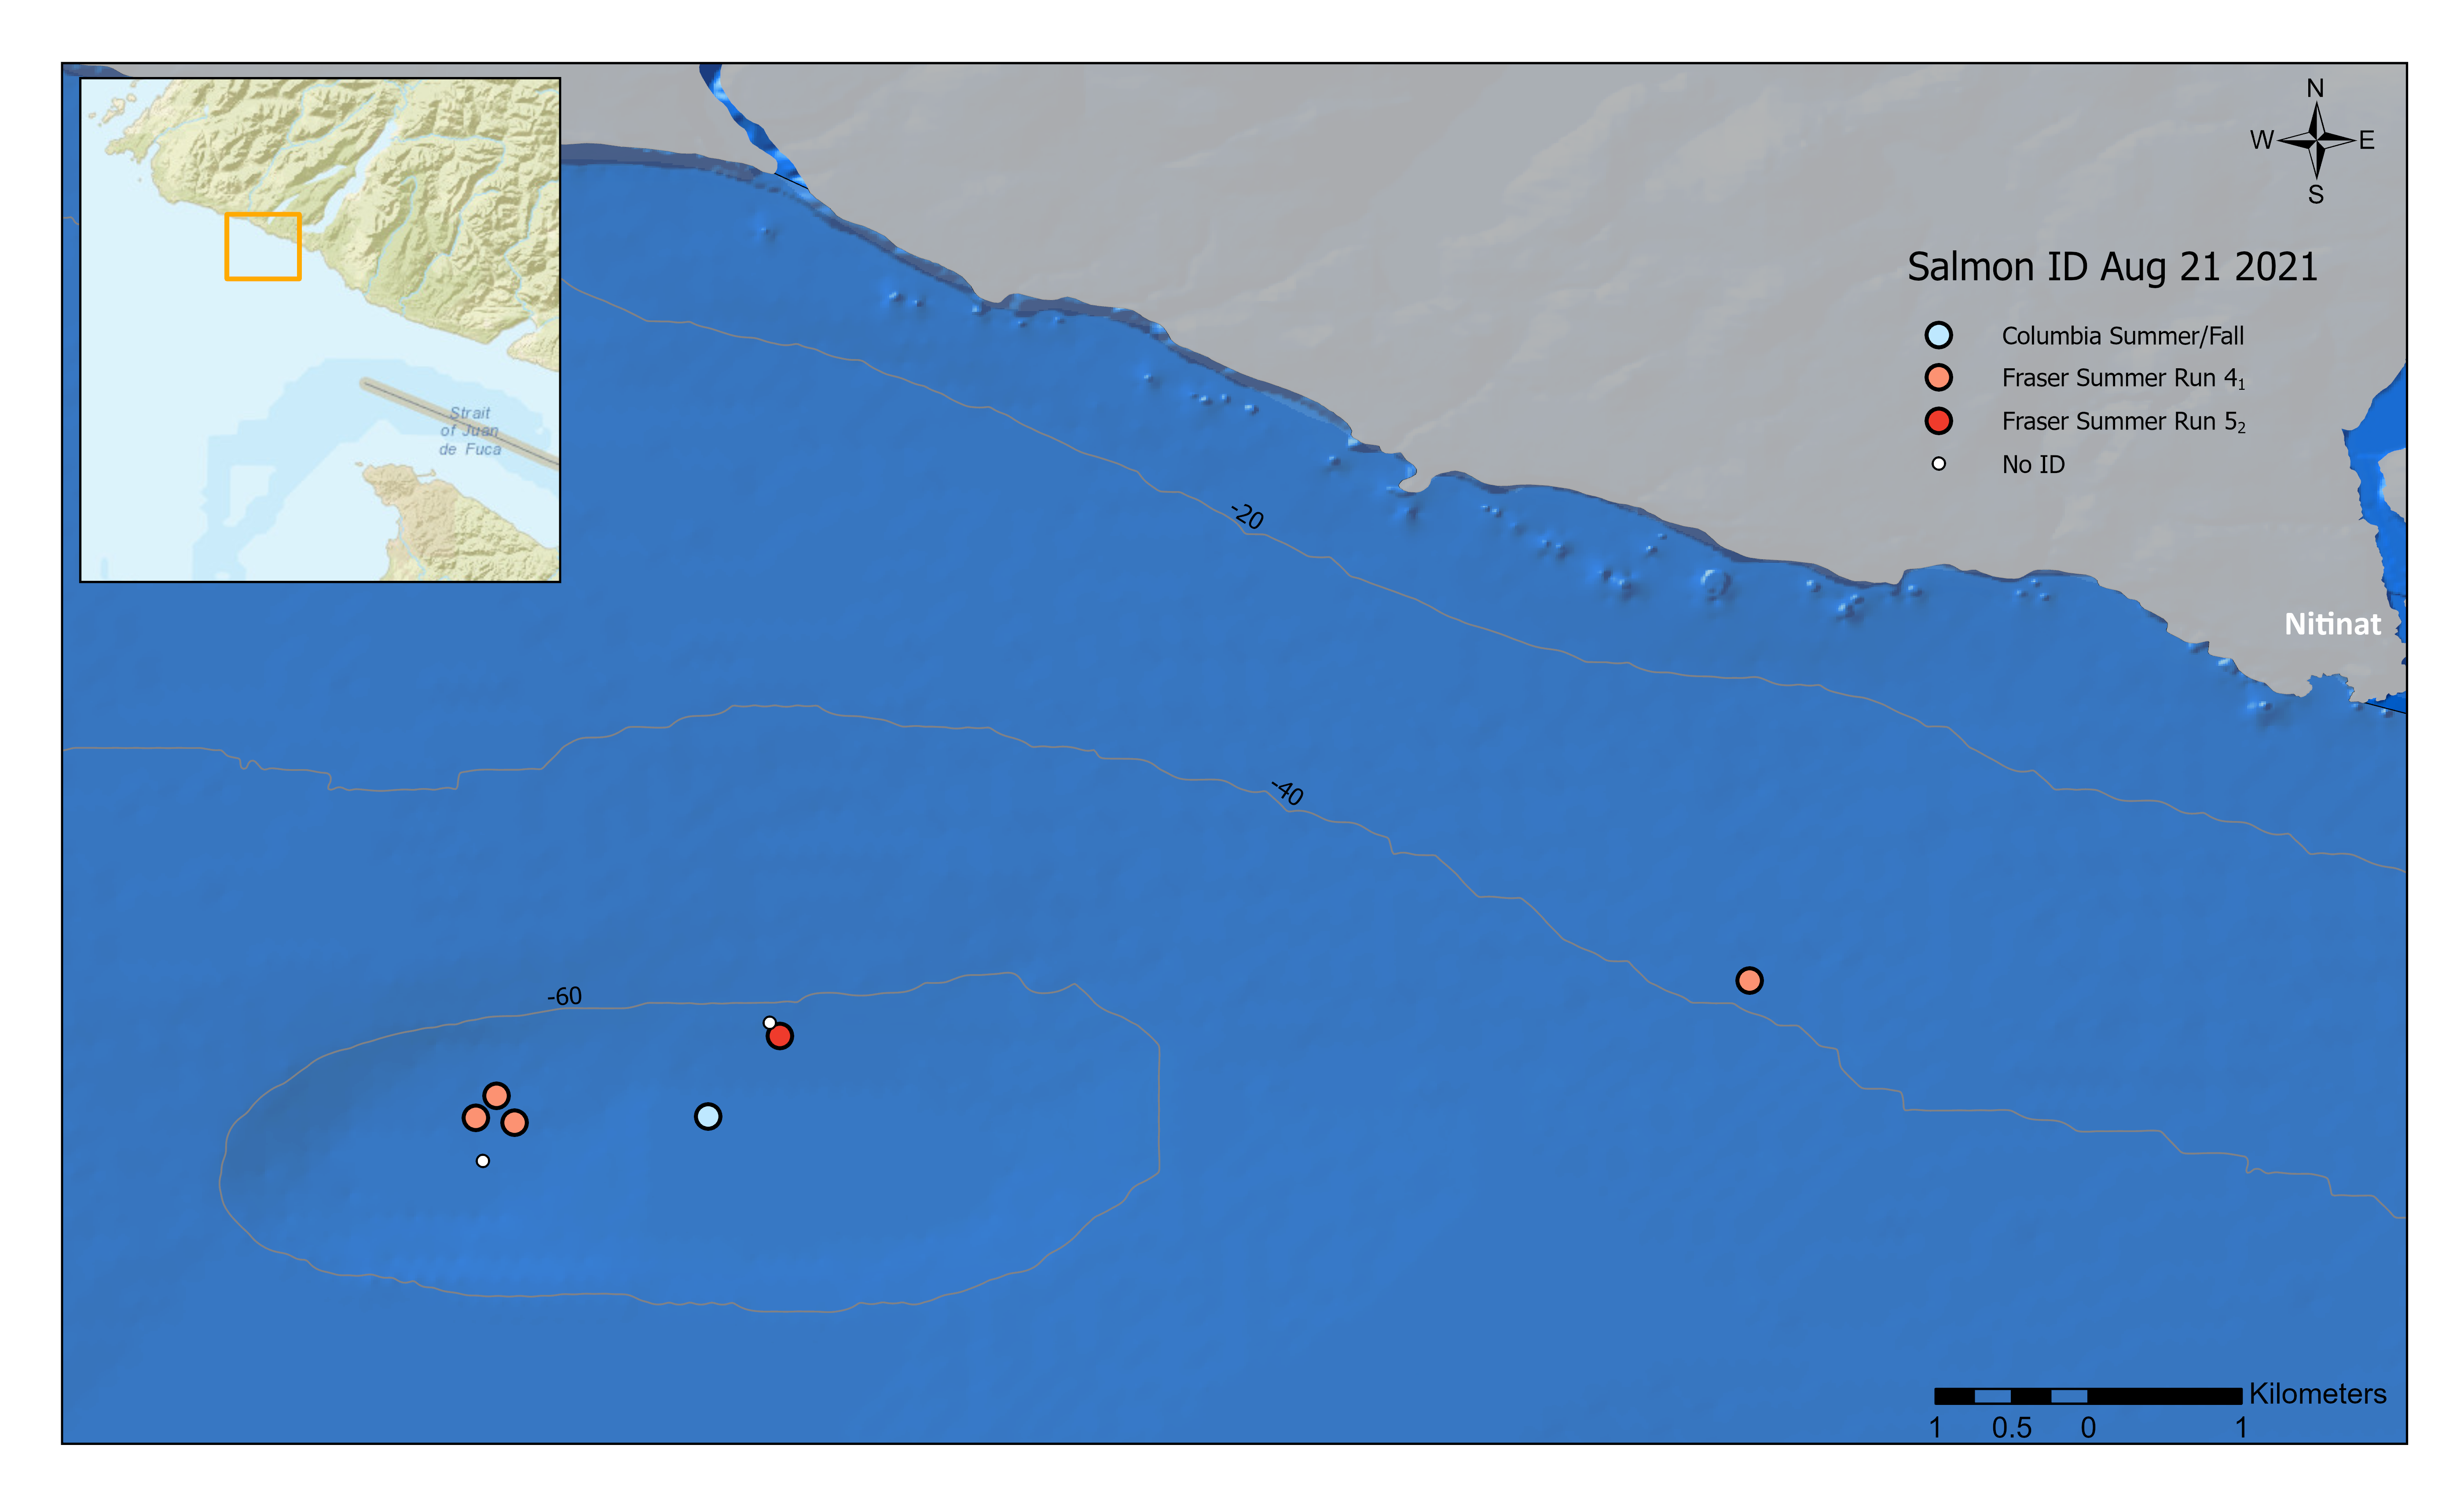
\includegraphics[width=5in]{figs/supp_figs/August21,2021Prey241217.png}}{Figure \ref{fig:prey-samples-2017}}
    \caption{Emplacements et identité du stock (probabilité la plus élevée pour un échantillon donné) des restes de proies des ERSN récoltés le 21 août 2017.}
    \label{fig:prey-samples-2017}
\end{figure}

\begin{figure}[htb]
    \centering
    \pdftooltip{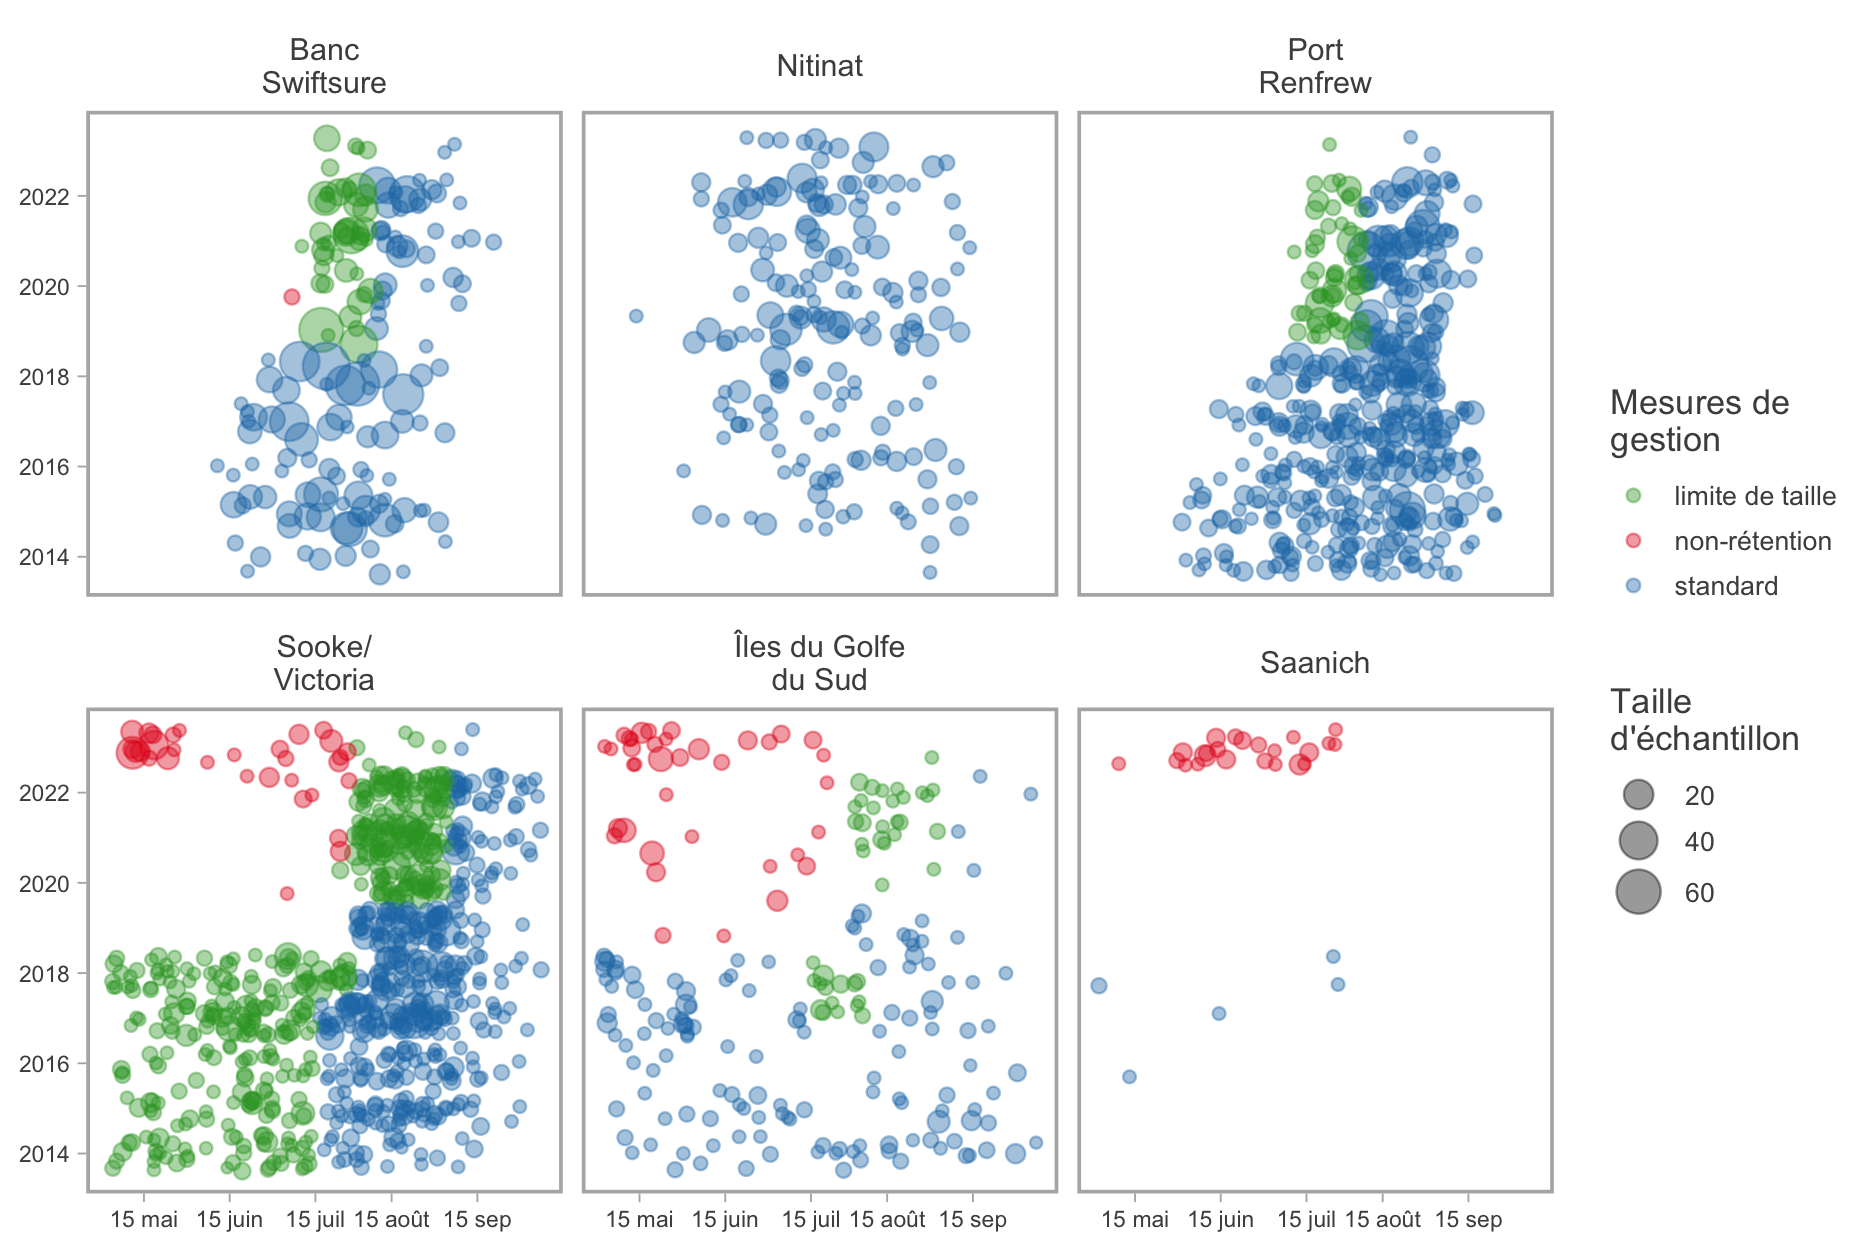
\includegraphics[width=5in]{figs/supp_figs/rec_temporal_sample_coverage_management.png}}{Figure \ref{fig:temporal-fishery-samples-management}}
    \caption{Distribution temporelle des échantillons de composition du stock de saumon chinook provenant des pêches récréatives entre mai et octobre, et mesures de gestion supplémentaires associées (couleurs). Les strates (panneaux) correspondent aux domaines spatiaux de la Figure \ref{fig:sampling-map}. Les échantillons prélevés pendant la non-rétention provenaient soit d'échantillons de pêcheurs passionnés de poissons remis à l'eau, soit de pêches de référence scientifiques. Notez que cette figure n'est pas destinée à saisir précisément les actions de gestion. Les limites de taille varient entre et à l'intérieur des strates et peuvent inclure à la fois des limites de taille minimale et maximale. Pour des informations détaillées sur les interventions spécifiques, consultez Dobson et al. 2020 pour les années antérieures à 2019 et les PGIP annuels (p. ex., MPO 2023). La taille des points est mise à l'échelle du nombre d'échantillons individuels collectés dans un lieu de pêche, une semaine et une année donnés. Les points ont été décalés pour maximiser la visibilité.}
    \label{fig:temporal-fishery-samples-management}
\end{figure}

\begin{figure}[htb]
    \centering
    \pdftooltip{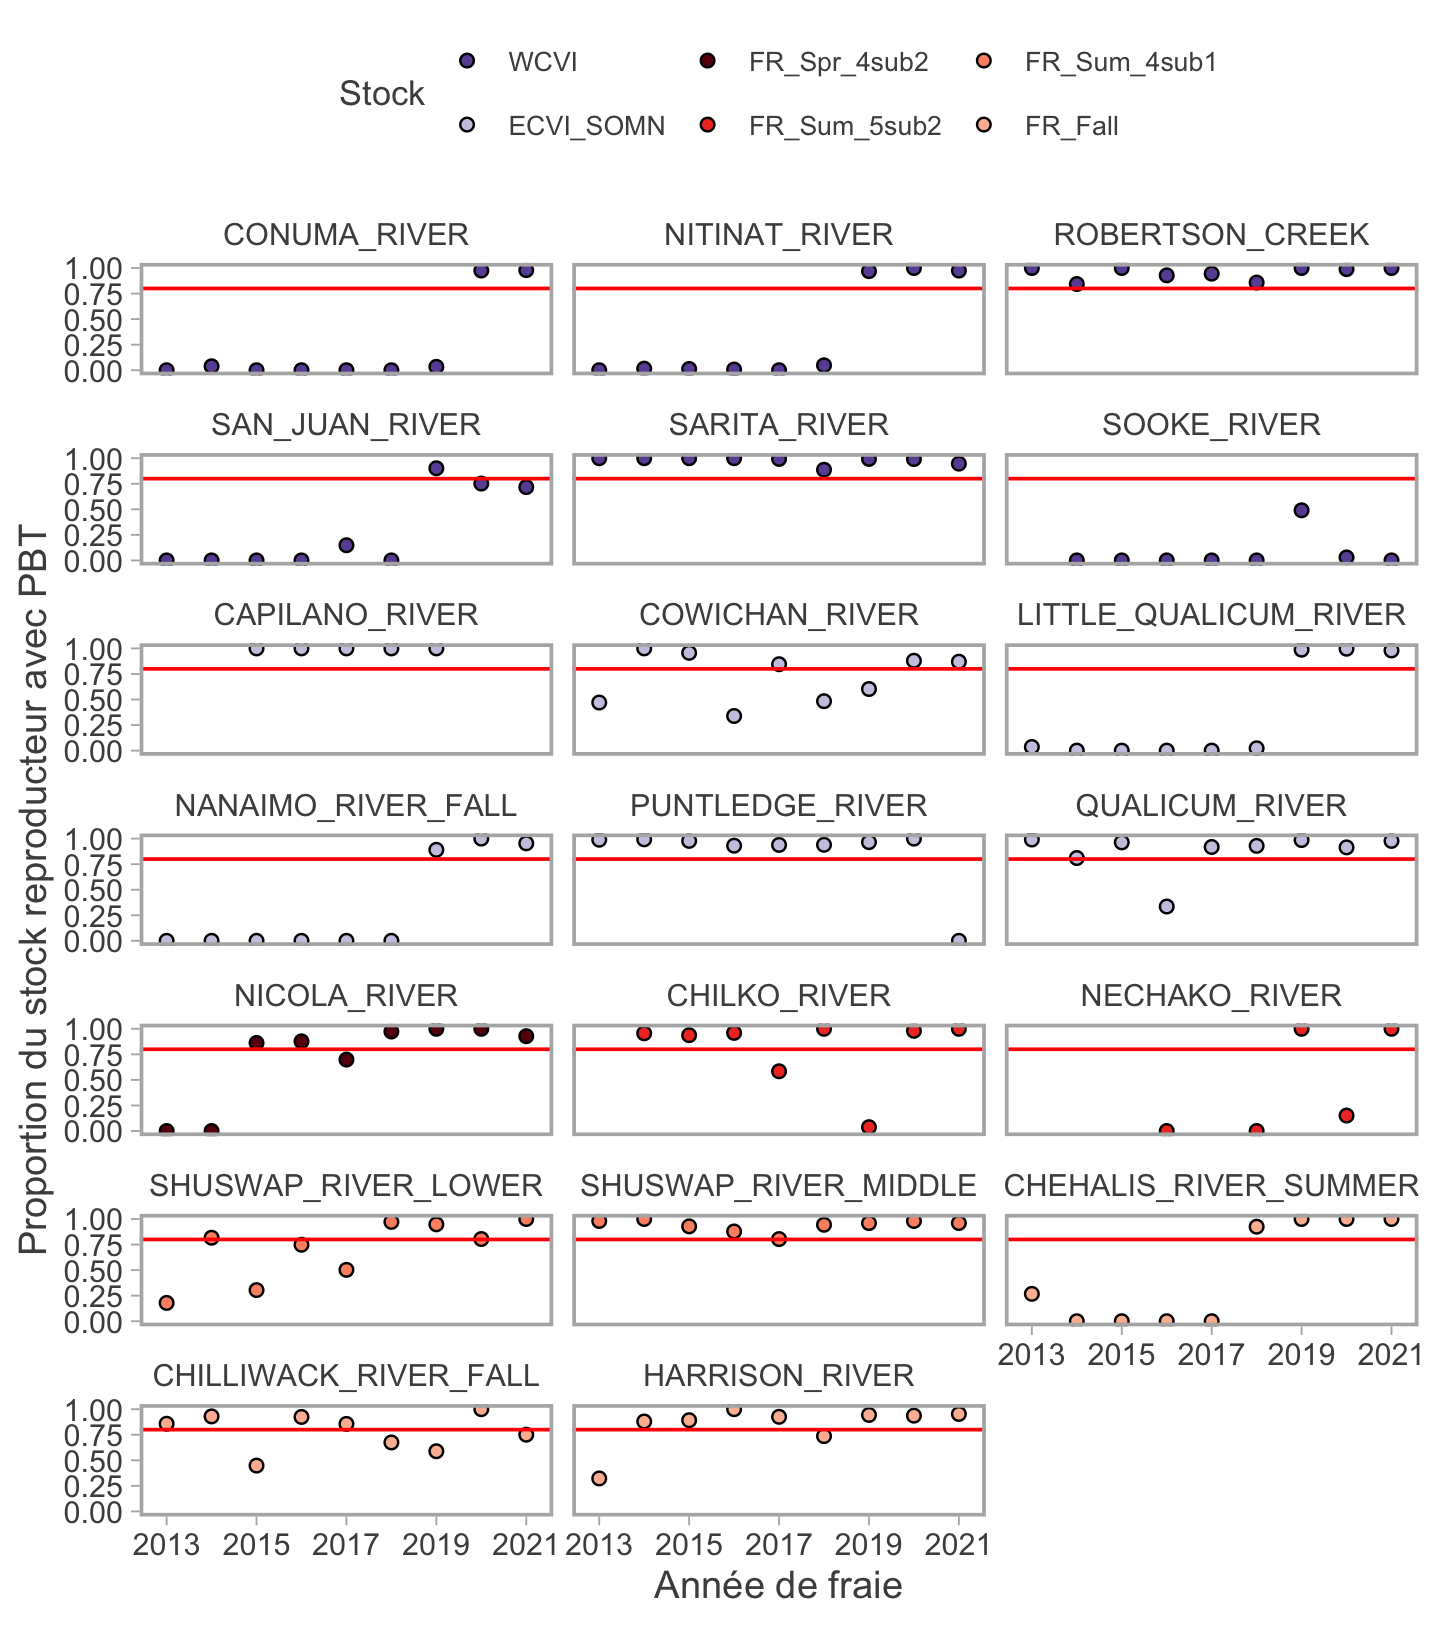
\includegraphics[width=5in]{figs/supp_figs/pbt_rate.png}}{Figure \ref{fig:pbt-coverage}}
    \caption{La proportion du stock géniteur de saumon chinook d'écloserie, par année de frai, incorporée dans la base de données EPF. La ligne rouge horizontale représente le seuil de marquage en deçà duquel les individus identifiés par GSI ont été assignés à une origine inconnue. Seules les principales installations d'amélioration (libérations annuelles moyennes supérieures à 140 000) avec des routes migratoires près de la zone d'étude sont présentées. Nechako et Chilko ont des tailles de libération annuelles moyennes inférieures à 140 000, mais sont présentées car les deux stocks étaient relativement abondants dans les pêches récréatives. Notez que les années de frai précèdent les années de retour d'au moins deux ans.}
    \label{fig:pbt-coverage}
\end{figure}

\begin{figure}[htb]
    \centering
    \pdftooltip{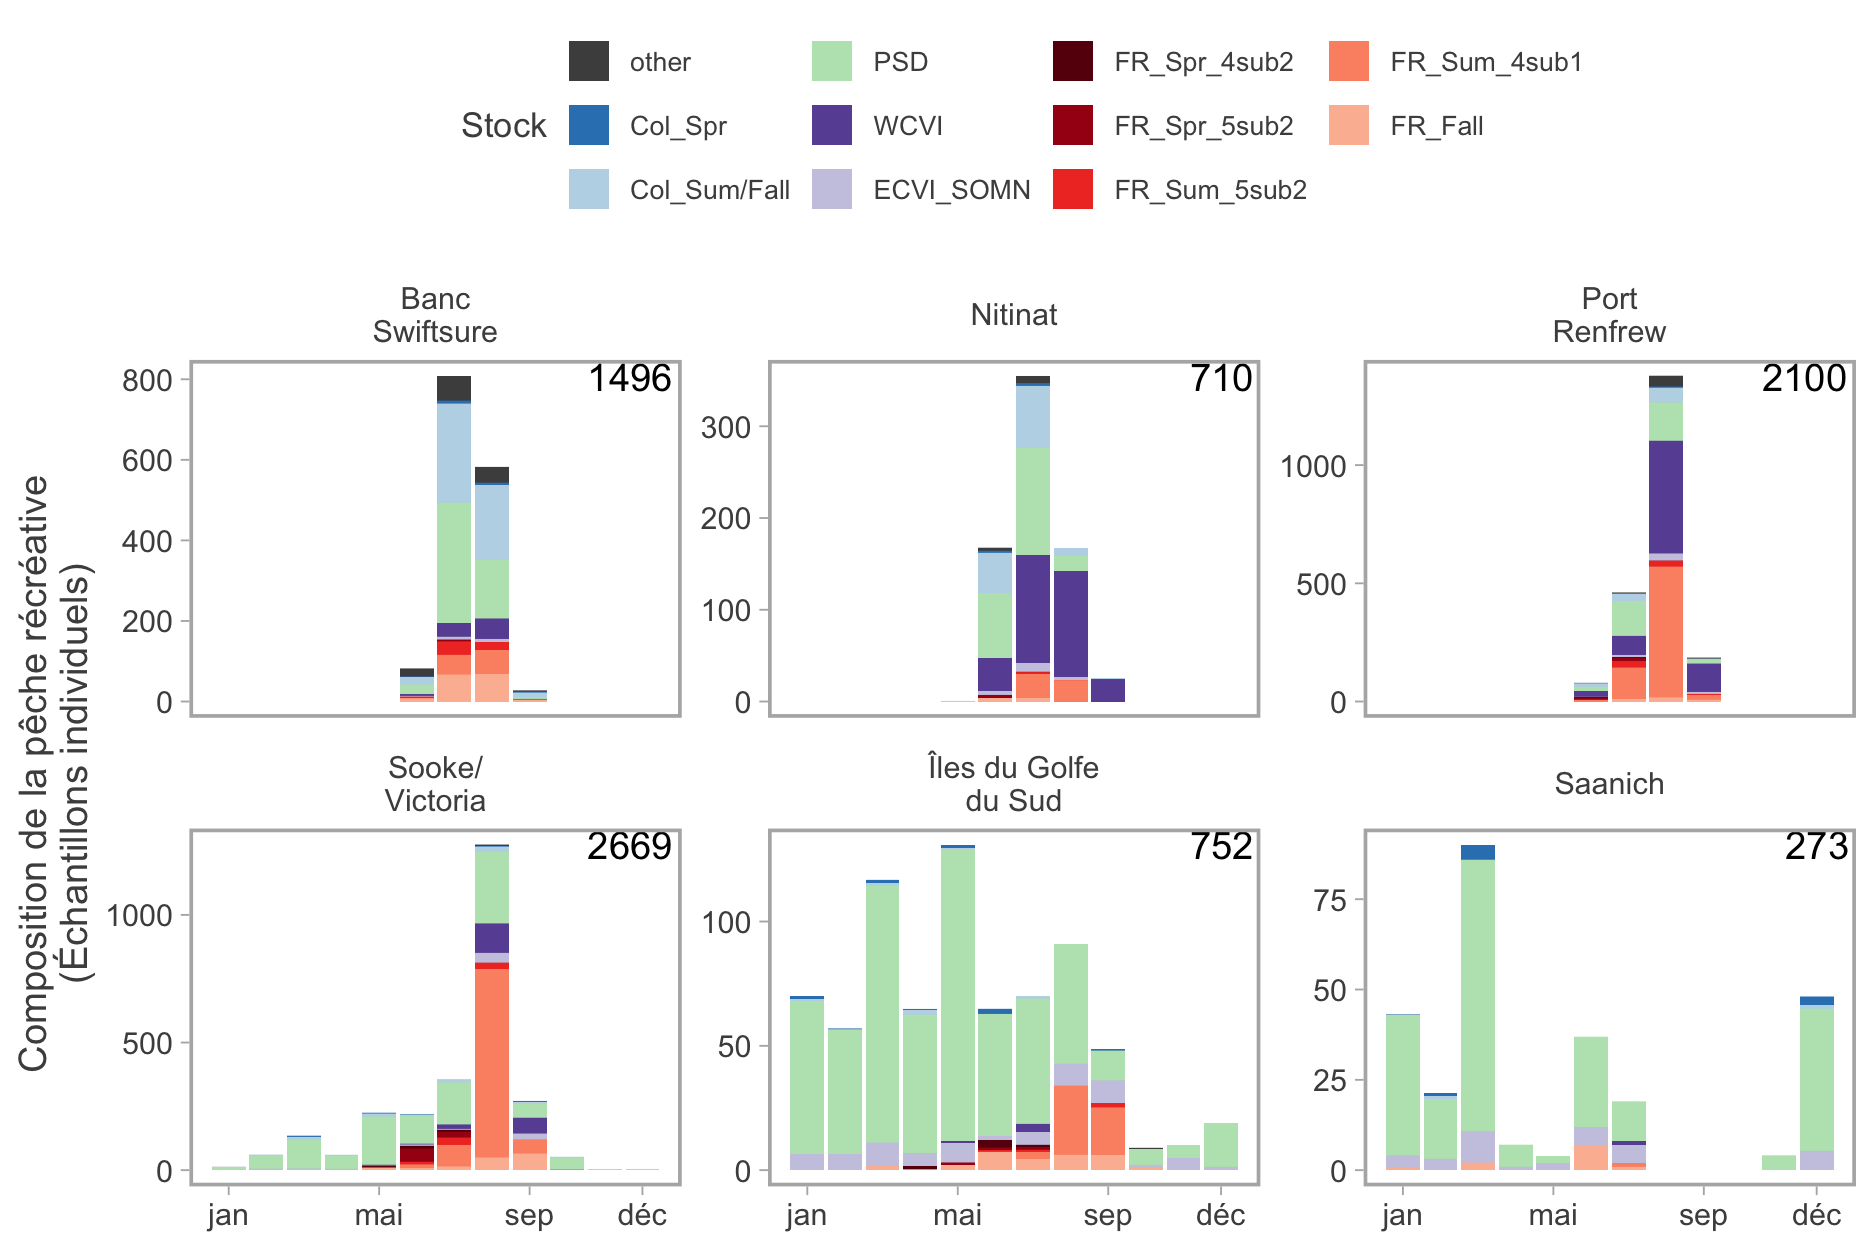
\includegraphics[width=5in]{figs/supp_figs/rec_monthly_comp_bar.png}}{Figure \ref{fig:bar-rec-full}}
    \caption{Composition mensuelle du stock d'échantillons de la pêche récréative de saumon chinook pendant tous les mois. Les strates (panneaux) correspondent aux domaines spatiaux de la Figure \ref{fig:sampling-map}. L'axe des y représente le nombre d'échantillons collectés dans un mois et une strate spatiale donnés. Les chiffres dans le coin supérieur droit de chaque panneau représentent la taille totale de l'échantillon dans chaque strate.}
    \label{fig:bar-rec-full}
\end{figure}

\begin{figure}[htb]
    \centering
    \pdftooltip{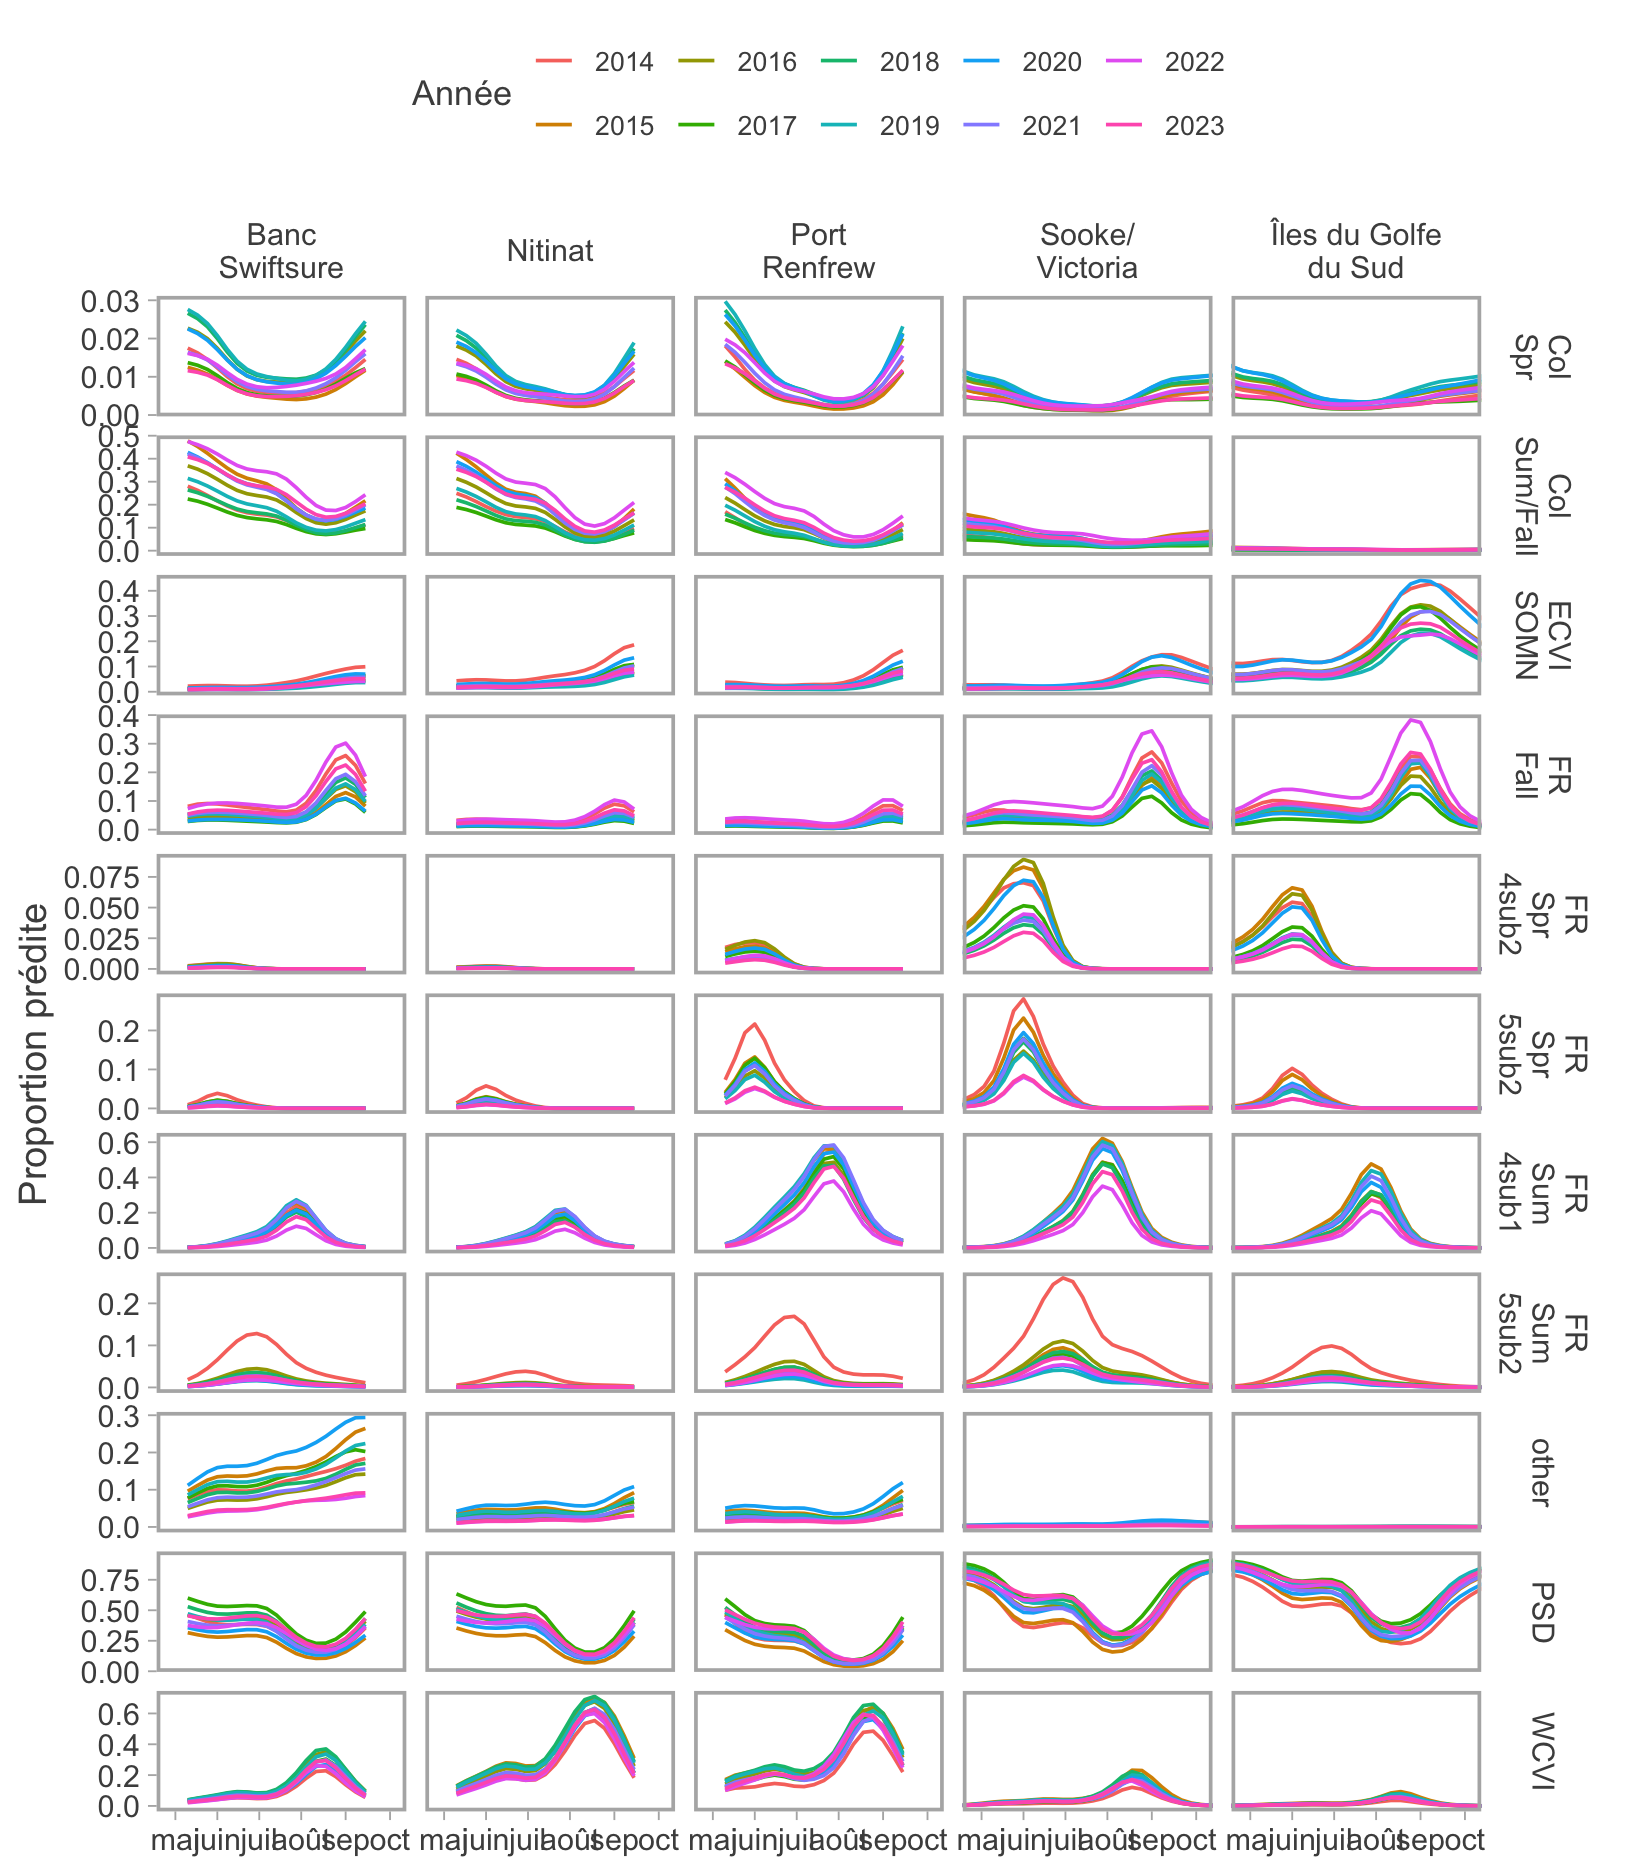
\includegraphics[width=5in]{figs/supp_figs/smooth_preds_chinook_year.png}}{Figure \ref{fig:smooth-pred-rec-year}}
    \caption{Composition moyenne prédite du stock spécifique à l'année. Les strates (panneaux) correspondent aux domaines spatiaux de la Figure \ref{fig:sampling-map}. Les intervalles de confiance ne sont pas montrés pour améliorer la lisibilité.}
    \label{fig:smooth-pred-rec-year}
\end{figure}

\begin{figure}[htb]
    \centering
    \pdftooltip{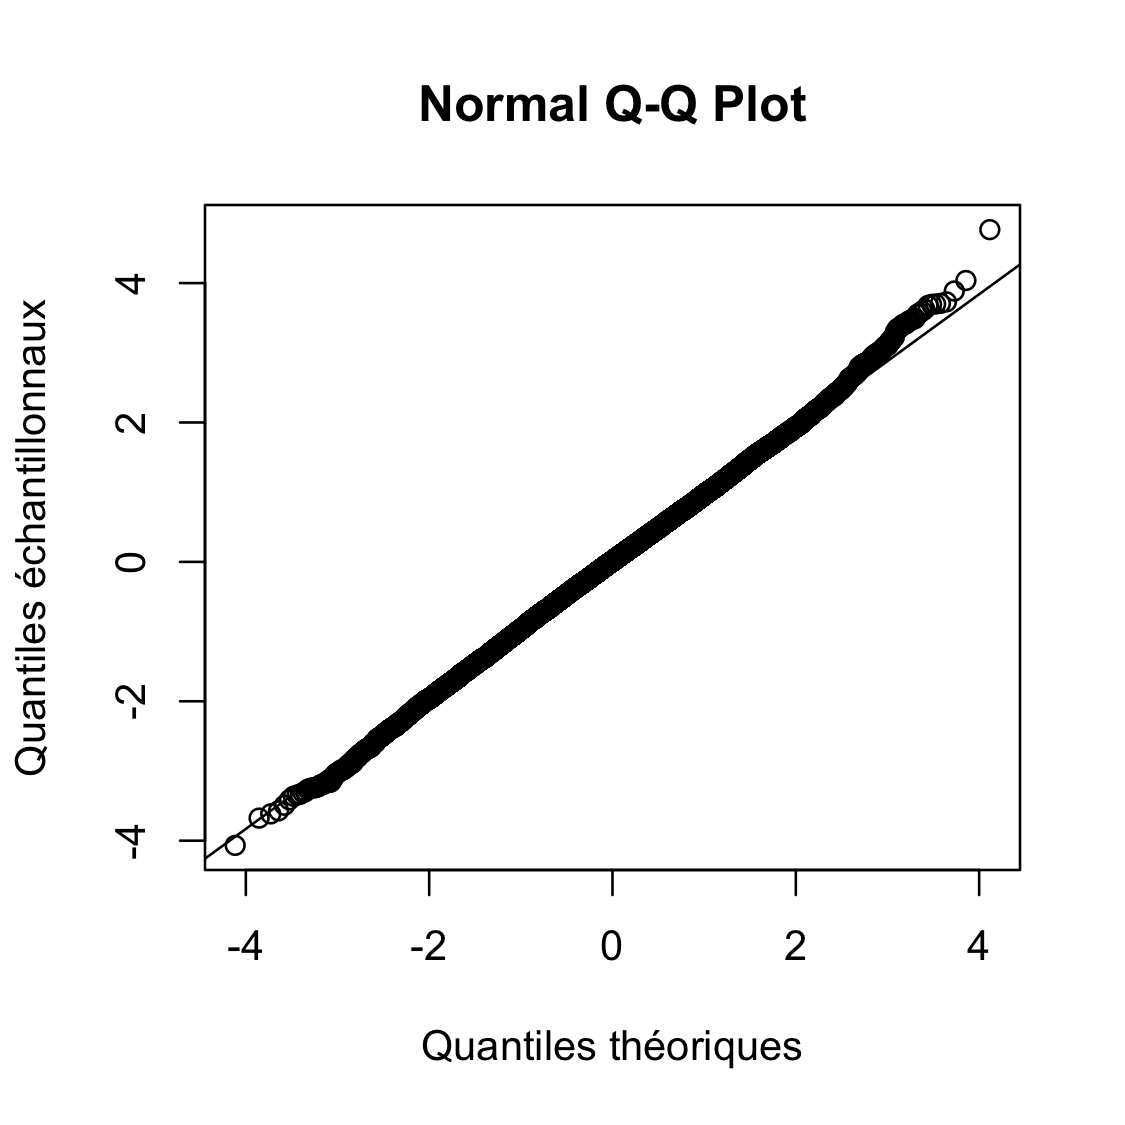
\includegraphics[width=5in]{figs/supp_figs/qq_plot_stock.png}}{Figure \ref{fig:qqplot-stock}}
    \caption{Résidus du modèle calculés à l'aide de tirages MCCM à partir de la distribution postérieure des prédictions avec des effets fixes aux estimations du maximum de vraisemblance et des effets aléatoires (c.-à-d., variance résiduelle) échantillonnés à partir de la distribution de Tweedie.}
    \label{fig:qqplot-stock}
\end{figure}

\begin{figure}[htb]
    \centering
    \pdftooltip{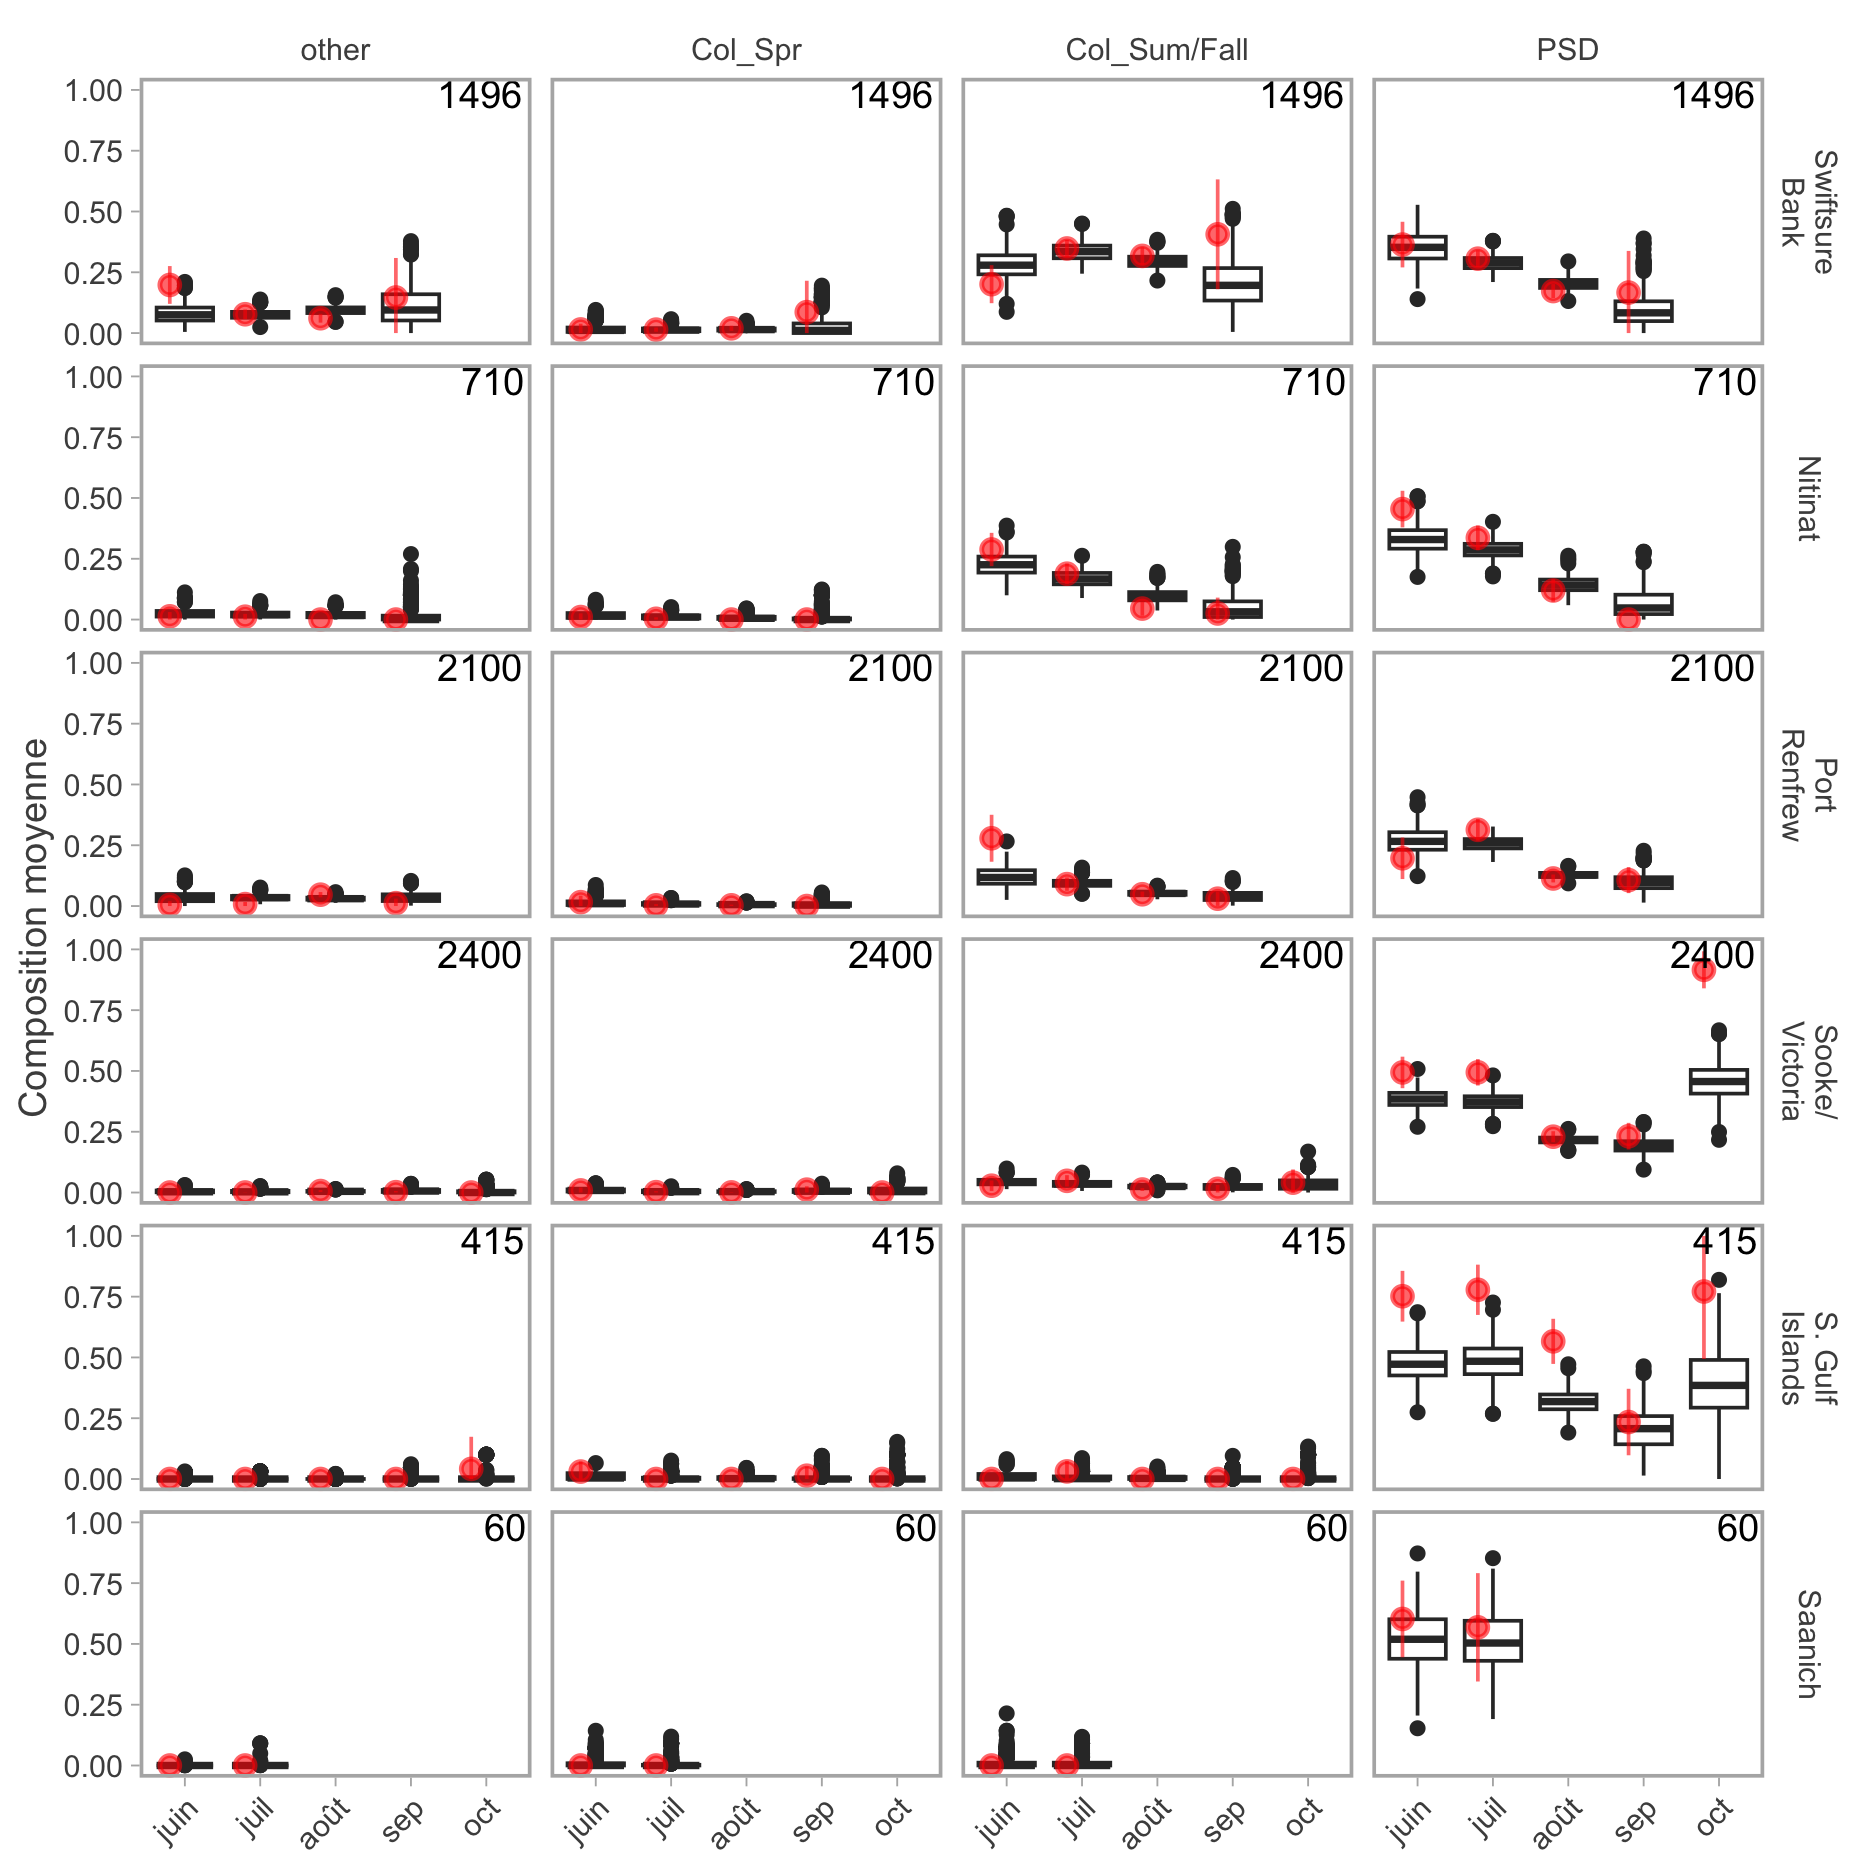
\includegraphics[width=5in]{figs/supp_figs/posterior_sims_stock1.png}}{Figure \ref{fig:posterior-stock1}}
    \caption{Composition moyenne simulée par modèle (diagrammes en boîte) et observée (points rouges) du stock pour les stocks «\,autre\,», Columbia Spring, Columbia Summer/Fall et Puget Sound. Les simulations représentent 500 tirages du modèle de Tweedie multivarié estimé, incluant la variance résiduelle, ajusté au jeu de données original. Les moustaches rouges représentent les intervalles de confiance approximatifs de 95\,\% associés à l'échantillon observé. Composition moyenne du stock calculée pour chaque strate et chaque mois. Les strates (panneaux) correspondent aux domaines spatiaux de la Figure \ref{fig:sampling-map}.}
    \label{fig:posterior-stock1}
\end{figure}

\begin{figure}[htb]
    \centering
    \pdftooltip{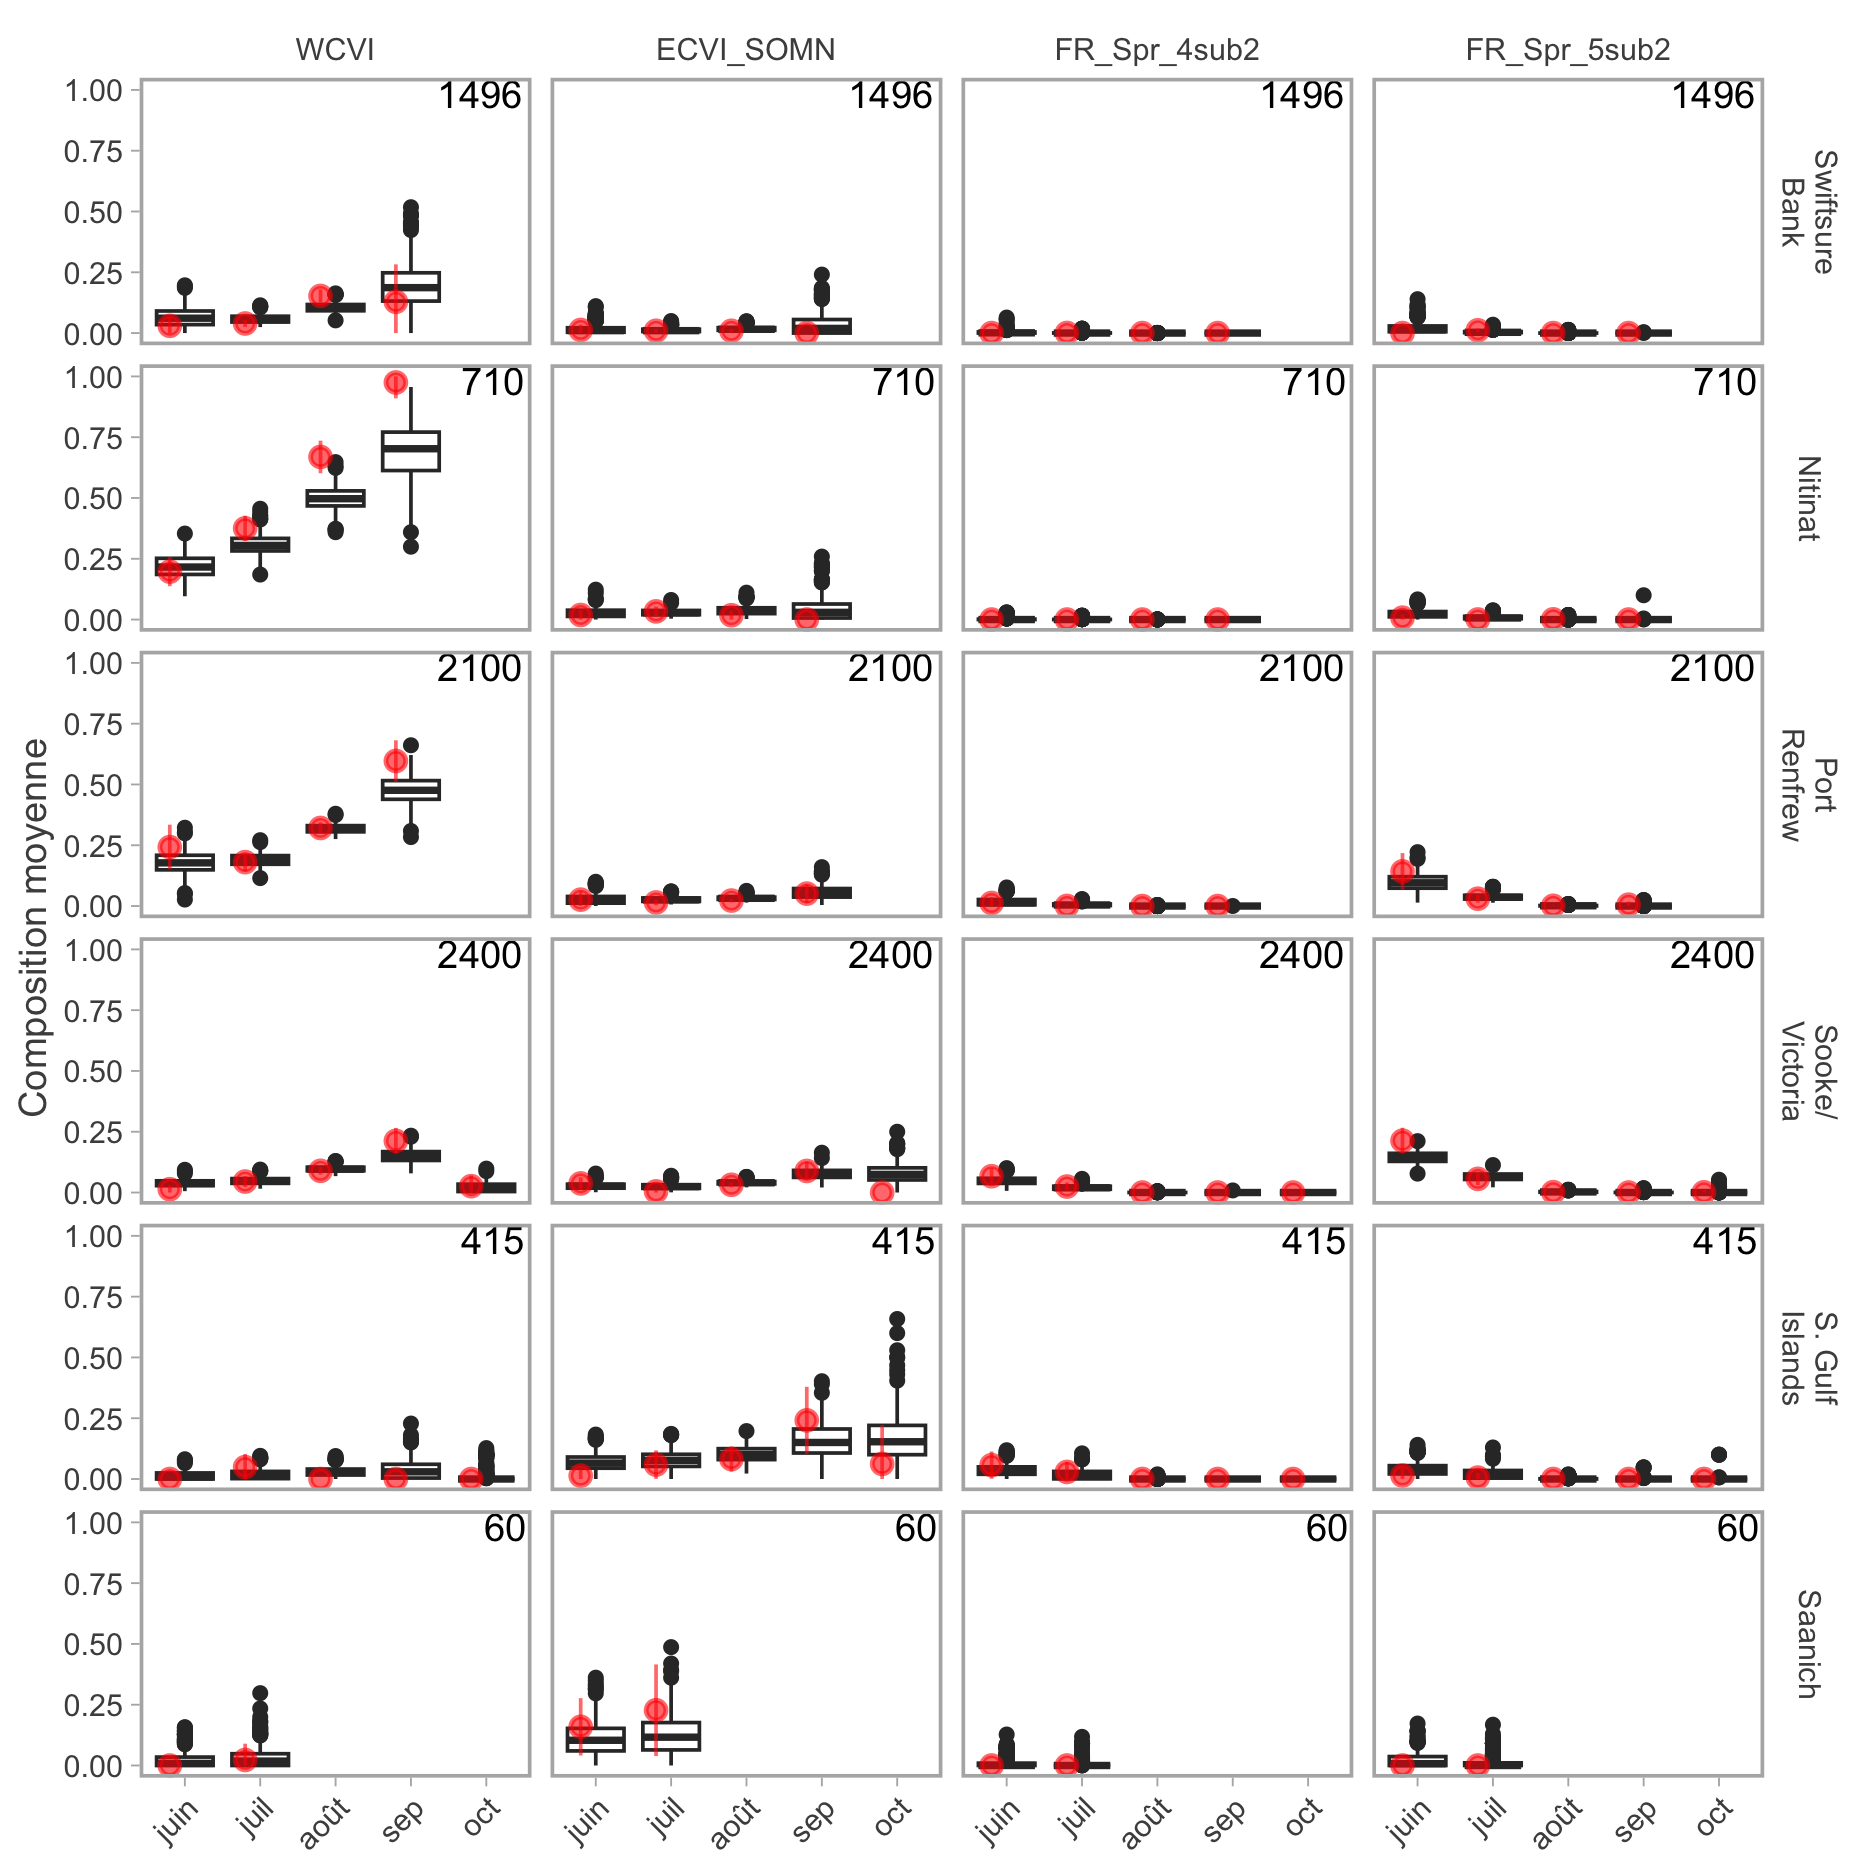
\includegraphics[width=5in]{figs/supp_figs/posterior_sims_stock2.png}}{Figure \ref{fig:posterior-stock2}}
    \caption{Composition moyenne simulée par modèle (diagrammes en boîte) et observée (points rouges) du stock pour les stocks de la côte ouest de l'île de Vancouver, de la côte est de l'île de Vancouver/continent méridional, Fraser Spring $4_2$ et Fraser Spring $5_2$. Les simulations représentent 500 tirages du modèle de Tweedie multivarié estimé, incluant la variance résiduelle, ajusté au jeu de données original. Les moustaches rouges représentent les intervalles de confiance approximatifs de 95\,\% associés à l'échantillon observé. Composition moyenne du stock calculée pour chaque strate et chaque mois. Les strates (panneaux) correspondent aux domaines spatiaux de la Figure \ref{fig:sampling-map}.}
    \label{fig:posterior-stock2}
\end{figure}

\begin{figure}[htb]
    \centering
    \pdftooltip{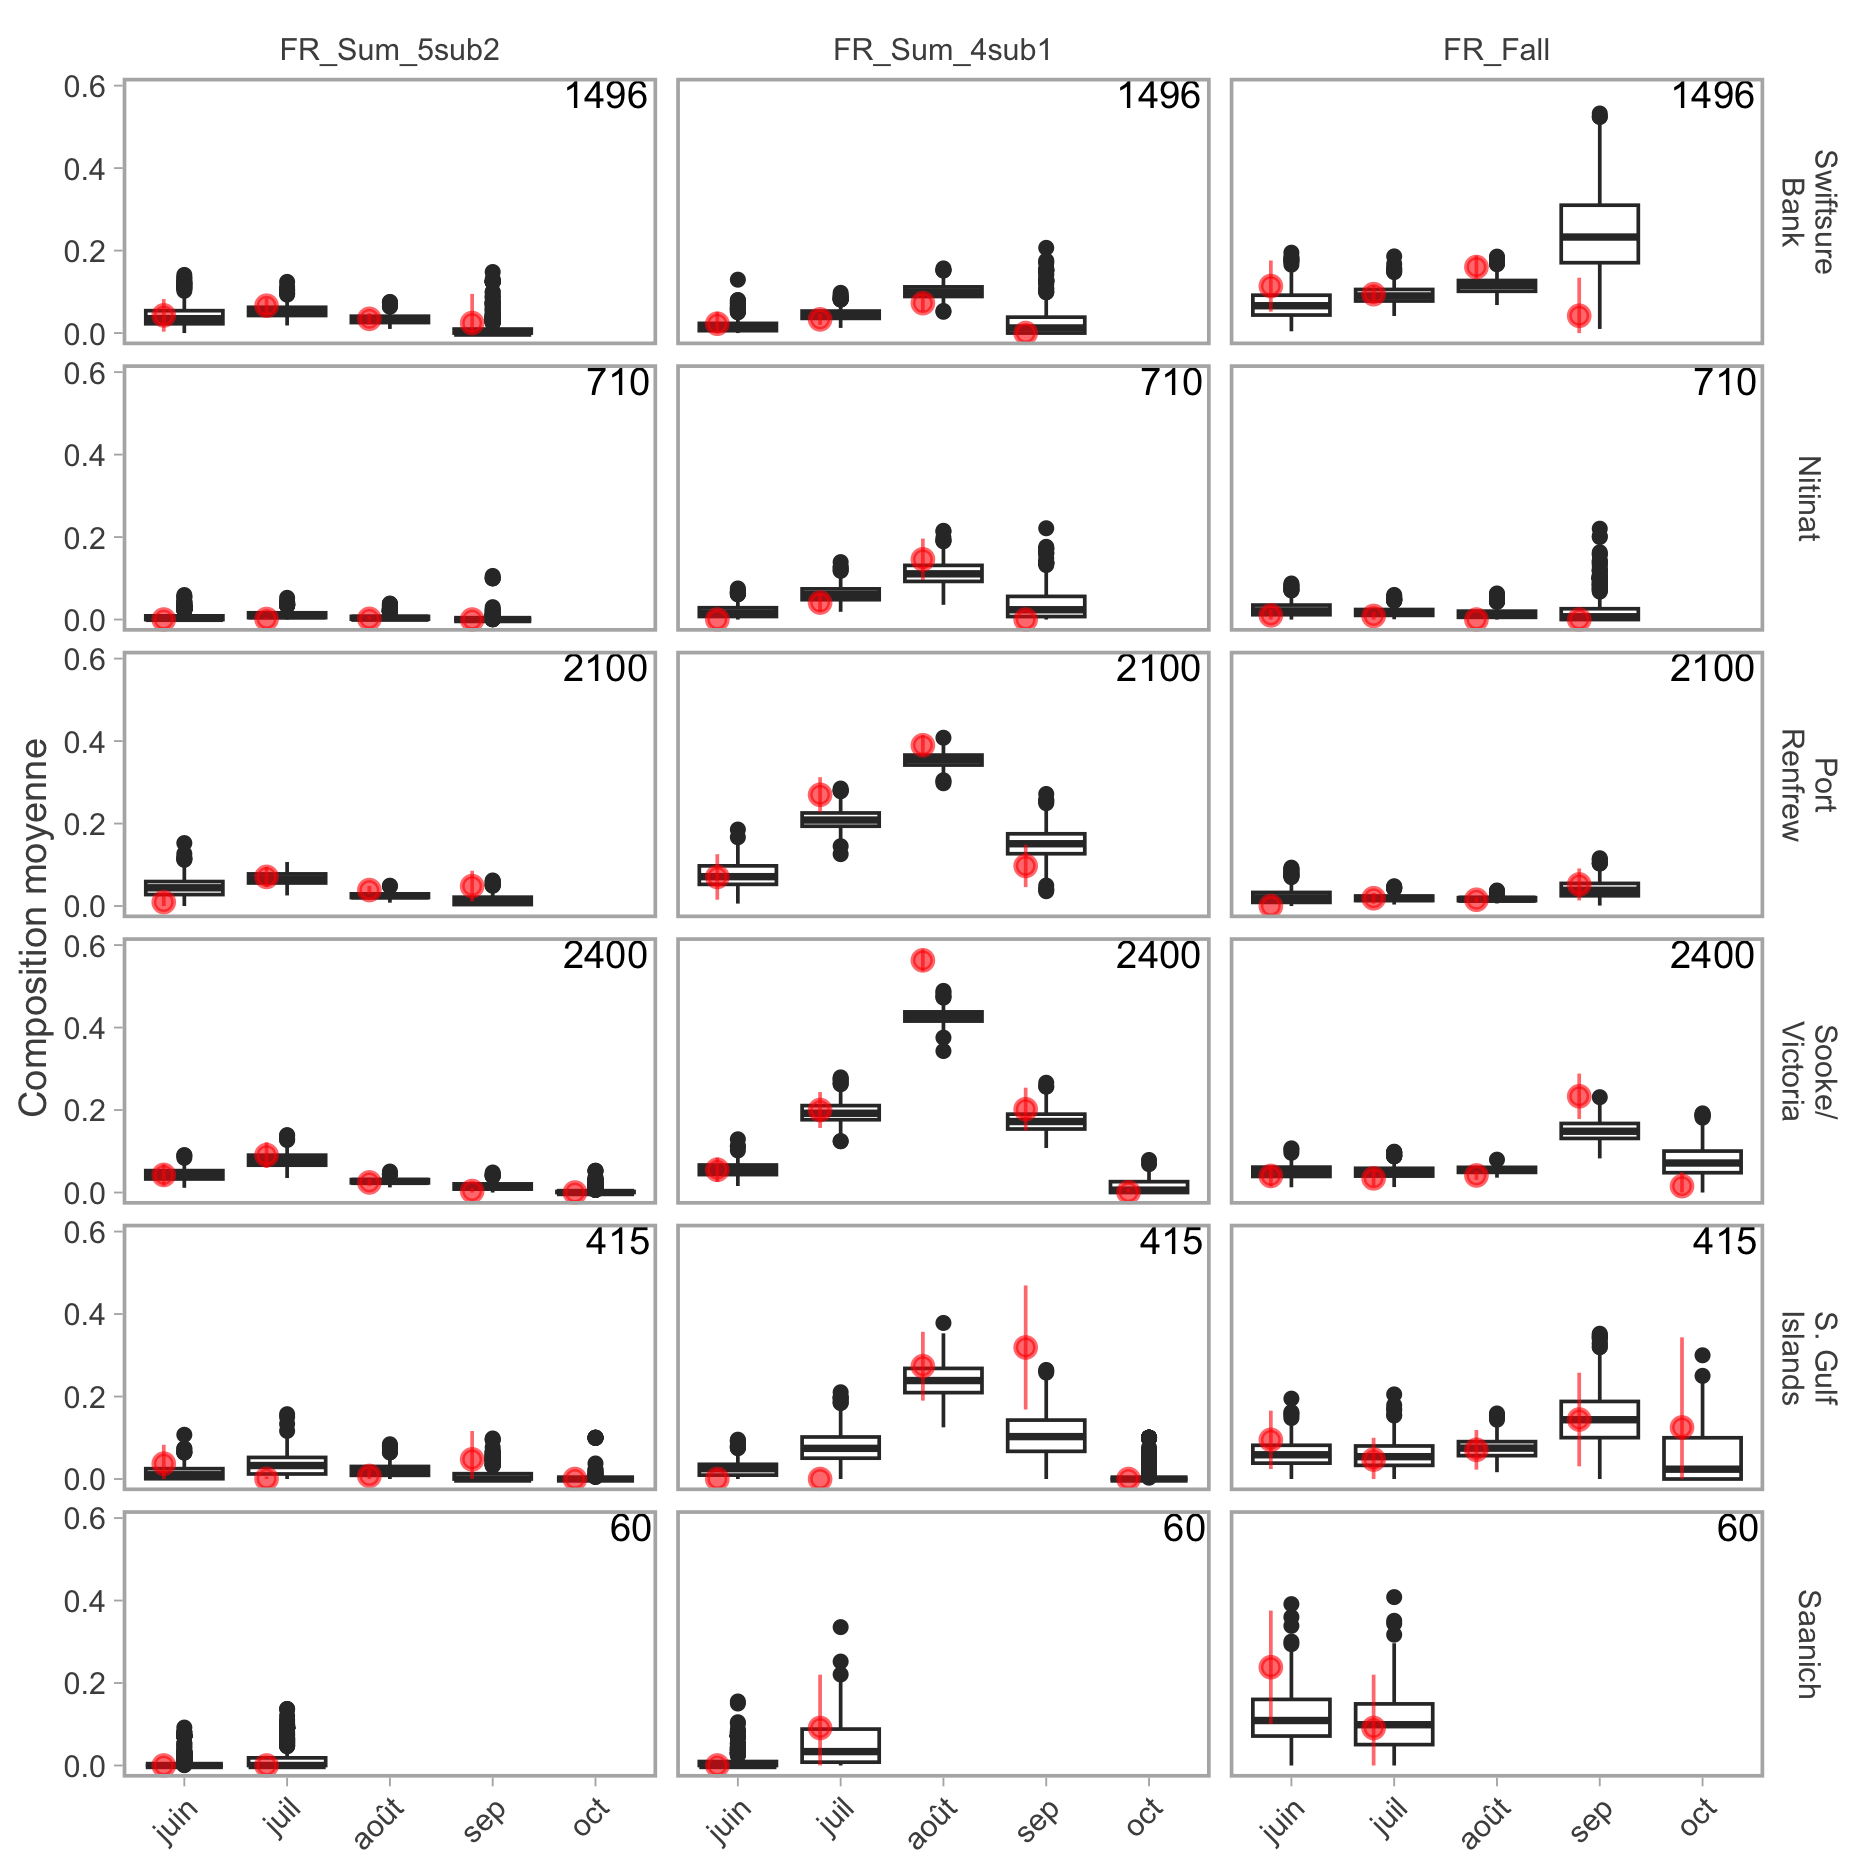
\includegraphics[width=5in]{figs/supp_figs/posterior_sims_stock3.png}}{Figure \ref{fig:posterior-stock3}}
    \caption{Composition moyenne simulée par modèle (diagrammes en boîte) et observée (points rouges) du stock pour les stocks Fraser Summer $5_2$, Fraser Summer $4_1$ et Fraser Fall. Les simulations représentent 500 tirages du modèle de Tweedie multivarié estimé, incluant la variance résiduelle, ajusté au jeu de données original. Les moustaches rouges représentent les intervalles de confiance approximatifs de 95\,\% associés à l'échantillon observé. Composition moyenne du stock calculée pour chaque strate et chaque mois. Les strates (panneaux) correspondent aux domaines spatiaux de la Figure \ref{fig:sampling-map}.}
    \label{fig:posterior-stock3}
\end{figure}

\begin{figure}[htb]
    \centering
    \pdftooltip{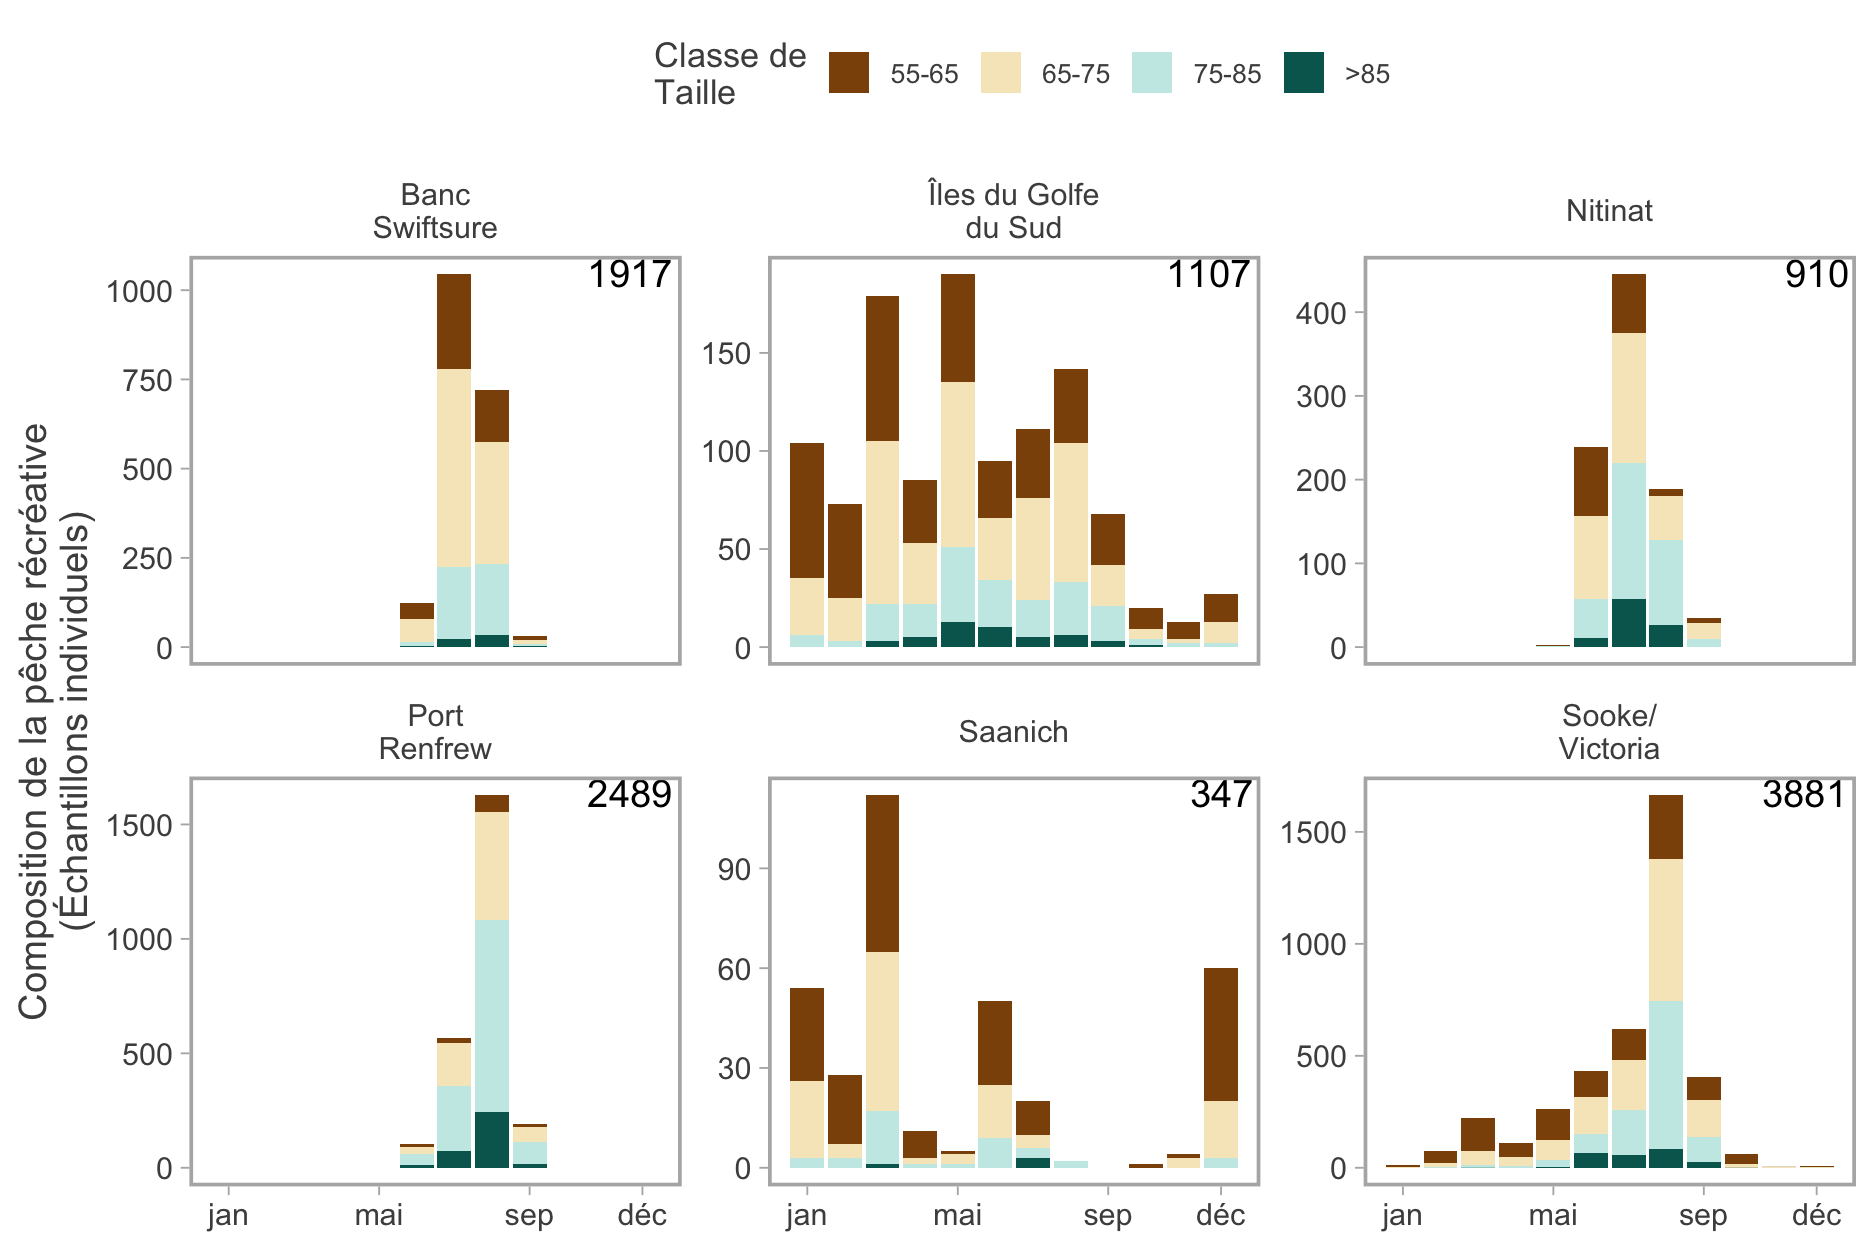
\includegraphics[width=5in]{figs/supp_figs/rec_monthly_size_bar.png}}{Figure \ref{fig:bar-rec-full-size}}
    \caption{Composition mensuelle de taille d'échantillons de la pêche récréative de saumon chinook pendant tous les mois. Les strates (panneaux) correspondent aux domaines spatiaux de la Figure \ref{fig:sampling-map}. L'axe des y représente le nombre d'échantillons collectés dans un mois et une strate spatiale donnés (notez que l'échelle diffère entre les strates). Les chiffres dans le coin supérieur droit de chaque panneau représentent la taille totale de l'échantillon dans chaque strate.}
    \label{fig:bar-rec-full-size}
\end{figure}

\begin{figure}[htb]
    \centering
    \pdftooltip{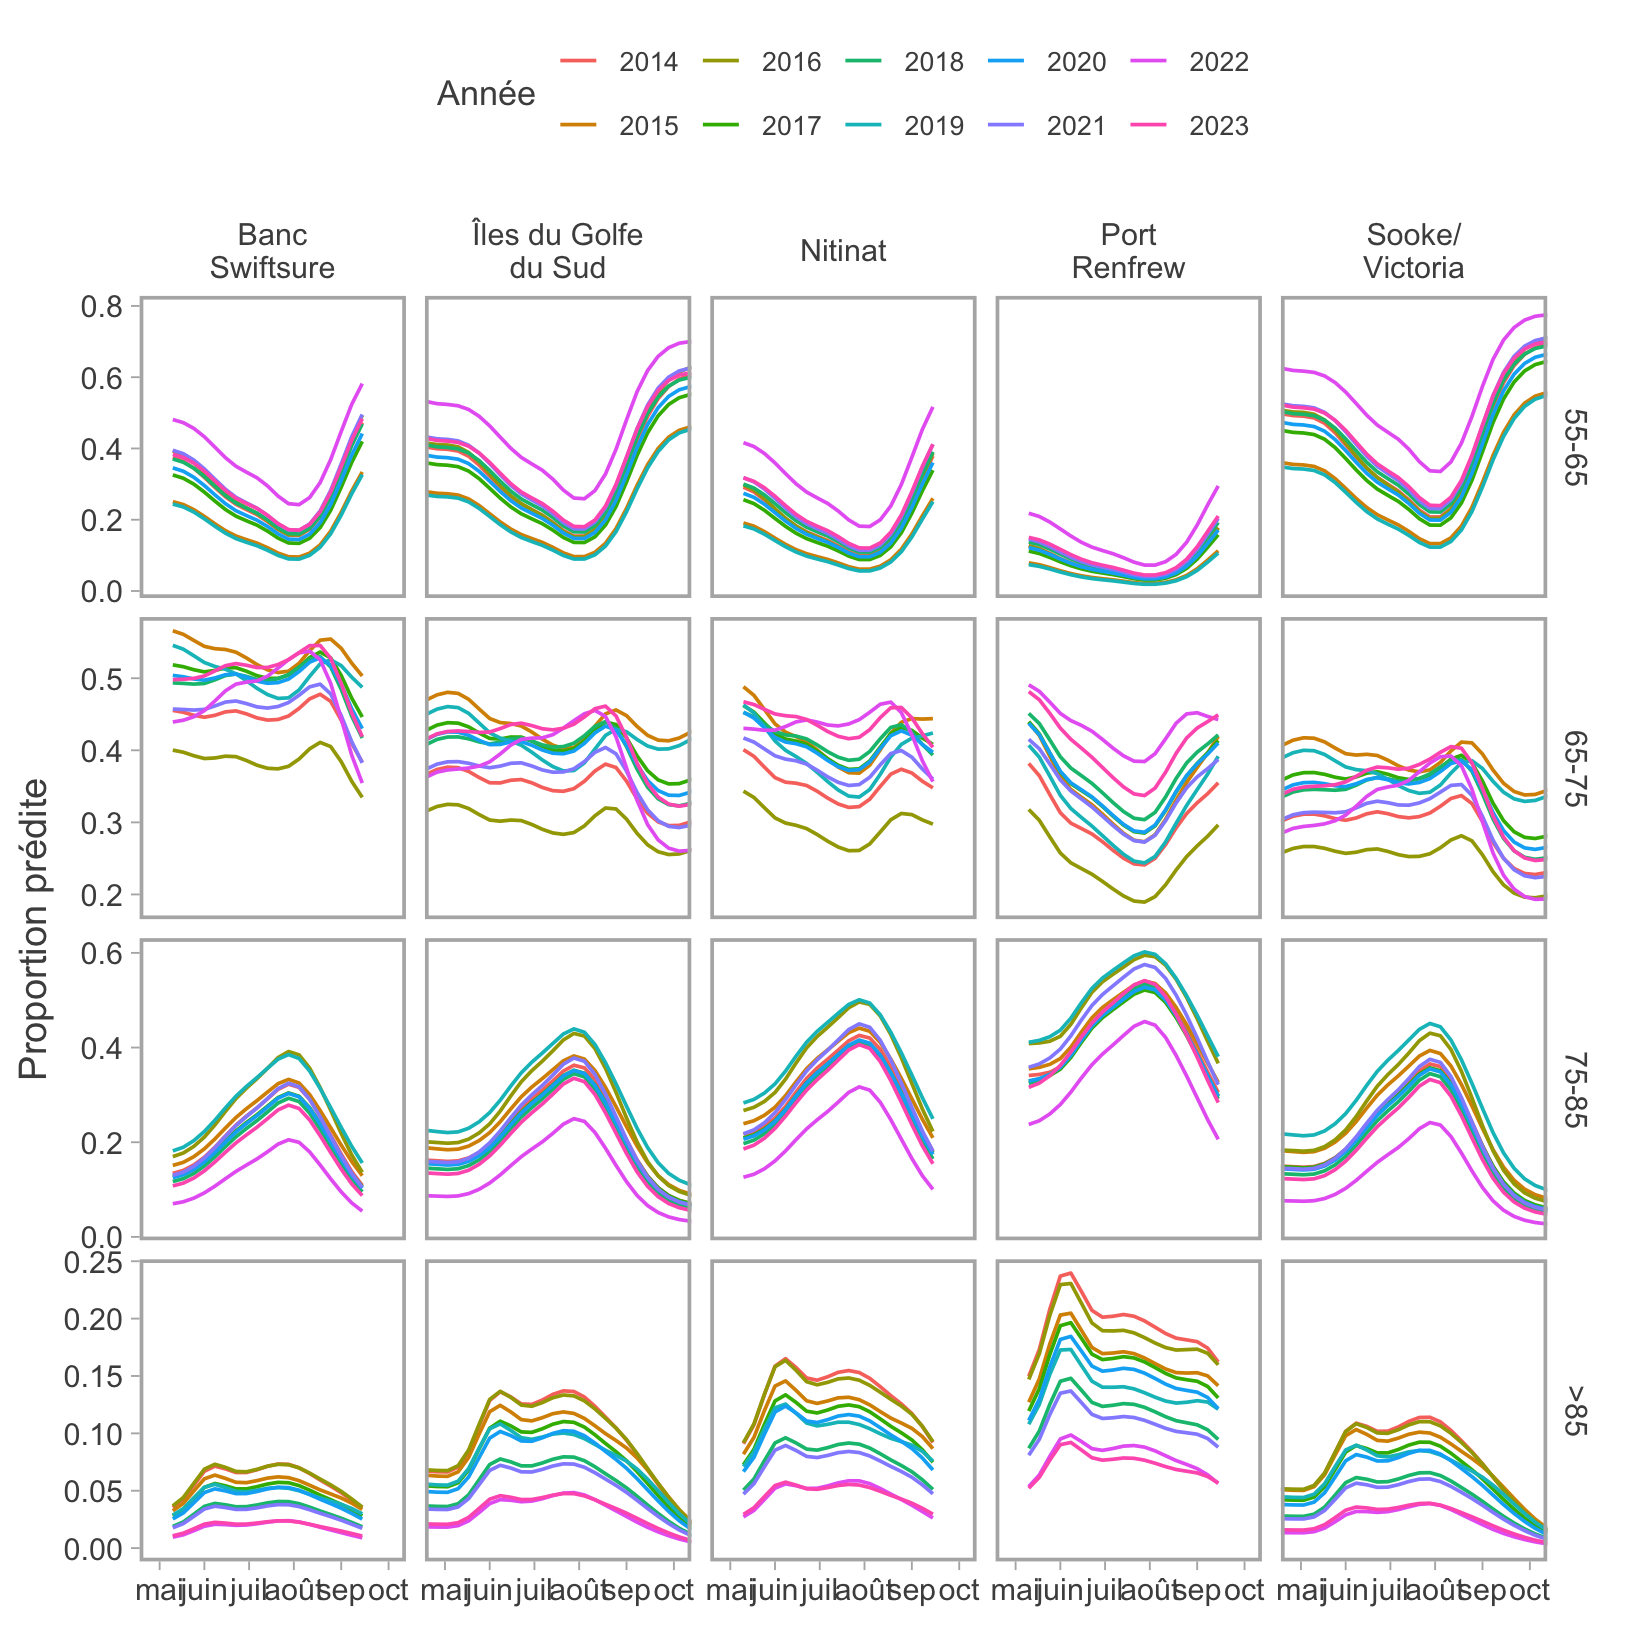
\includegraphics[width=5in]{figs/supp_figs/size_smooth_preds_chinook_year.png}}{Figure \ref{fig:size-smooth-pred-rec-year}}
    \caption{Composition moyenne prédite de taille spécifique à l'année. Les strates (panneaux) correspondent aux domaines spatiaux de la Figure \ref{fig:sampling-map}. Les intervalles de confiance ne sont pas montrés pour améliorer la lisibilité.}
    \label{fig:size-smooth-pred-rec-year}
\end{figure}

\begin{figure}[htb]
    \centering
    \pdftooltip{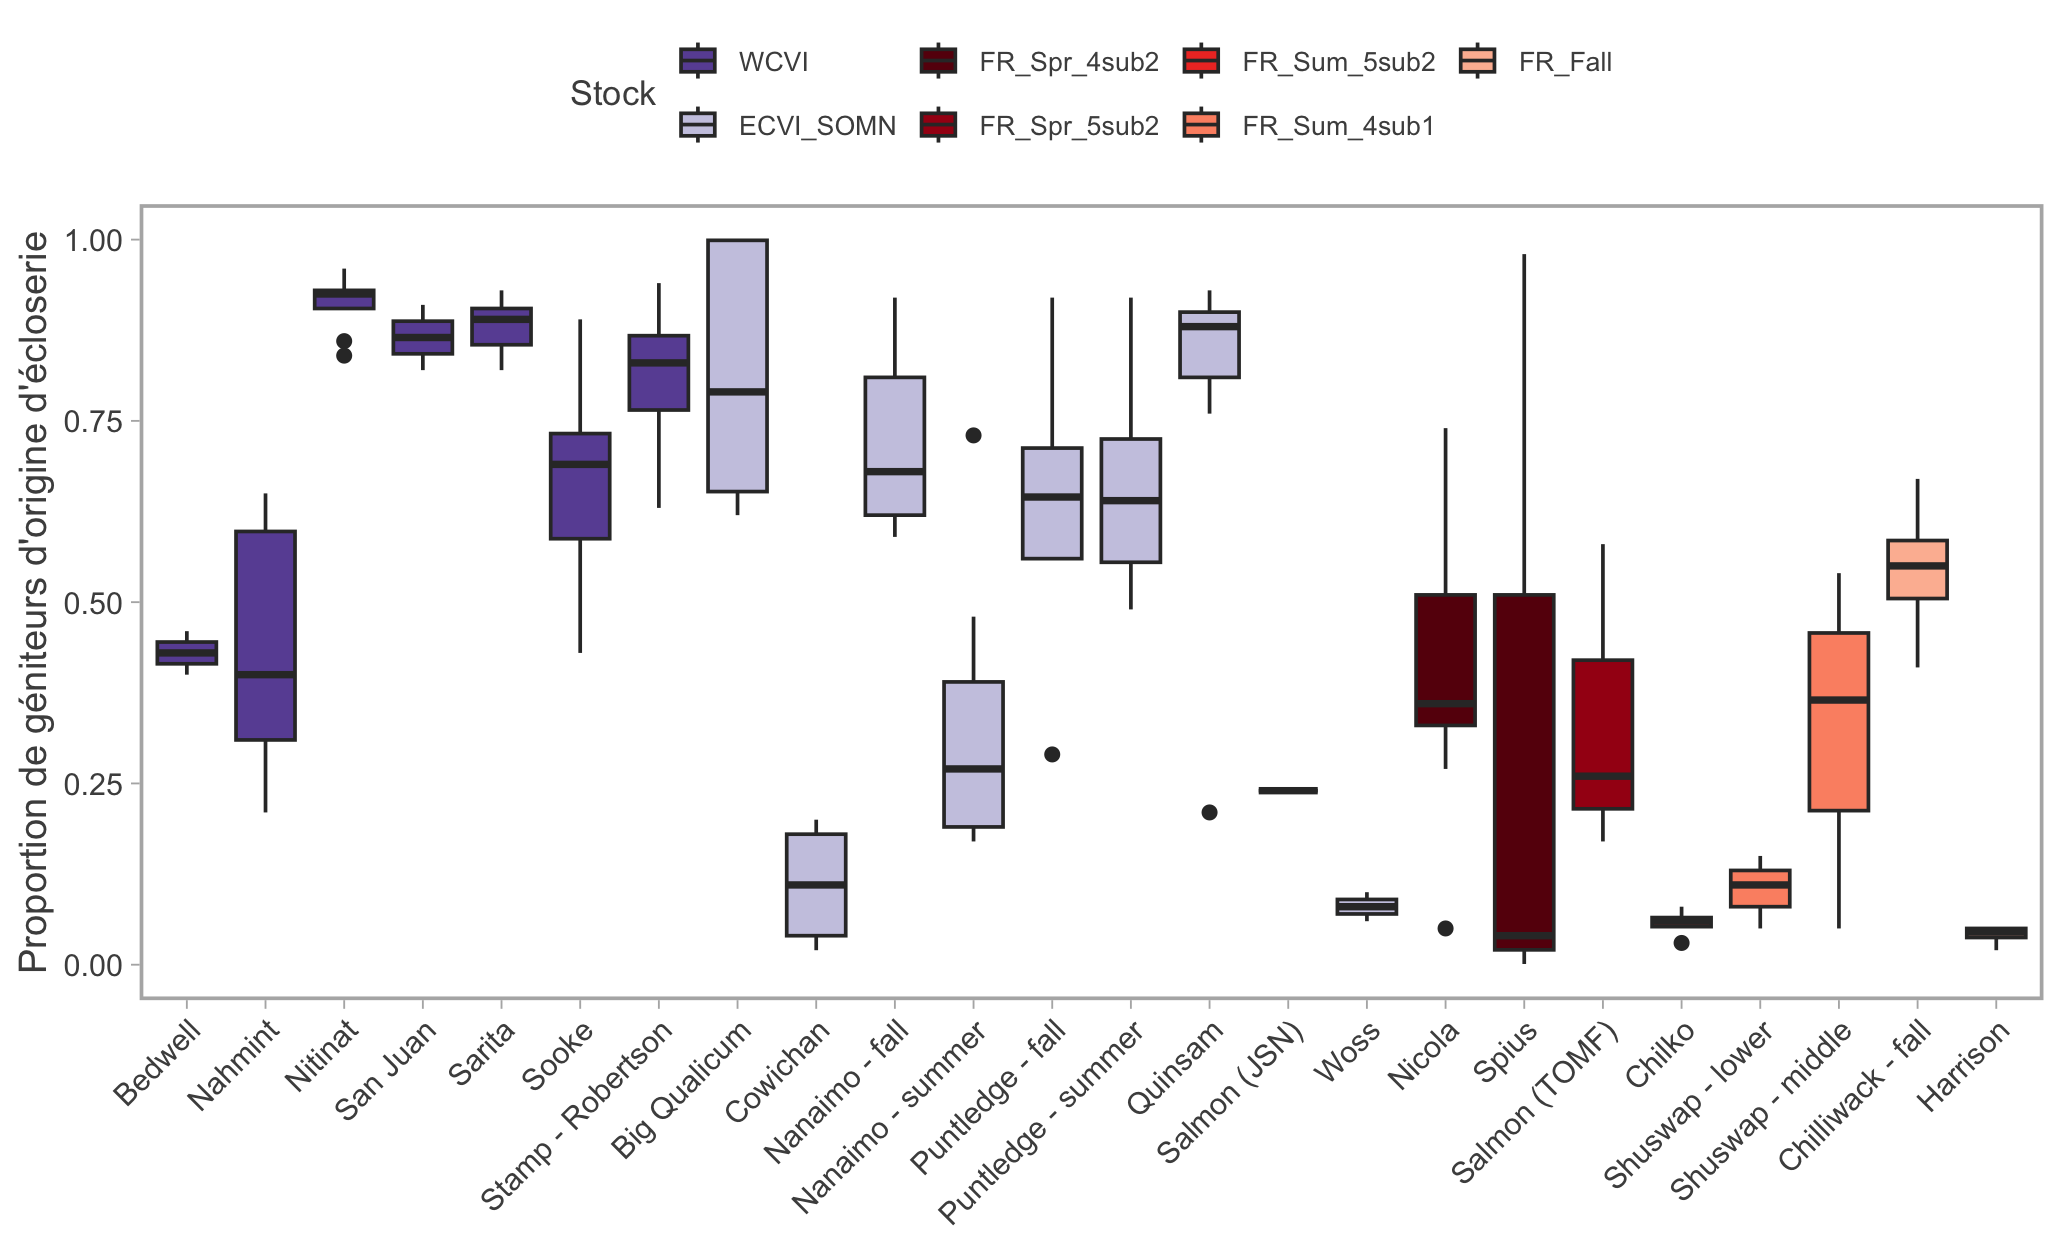
\includegraphics[width=5in]{figs/supp_figs/phos_box.png}}{Figure \ref{fig:box-phos}}
    \caption{La proportion estimée de géniteurs d'origine d'écloserie pour un sous-ensemble de populations de saumon chinook canadiennes. Les diagrammes en boîte représentent la variabilité entre les années (2014-2022). Les couleurs représentent les stocks d'origine canadienne.}
    \label{fig:box-phos}
\end{figure}

\begin{figure}[htb]
    \centering
    \pdftooltip{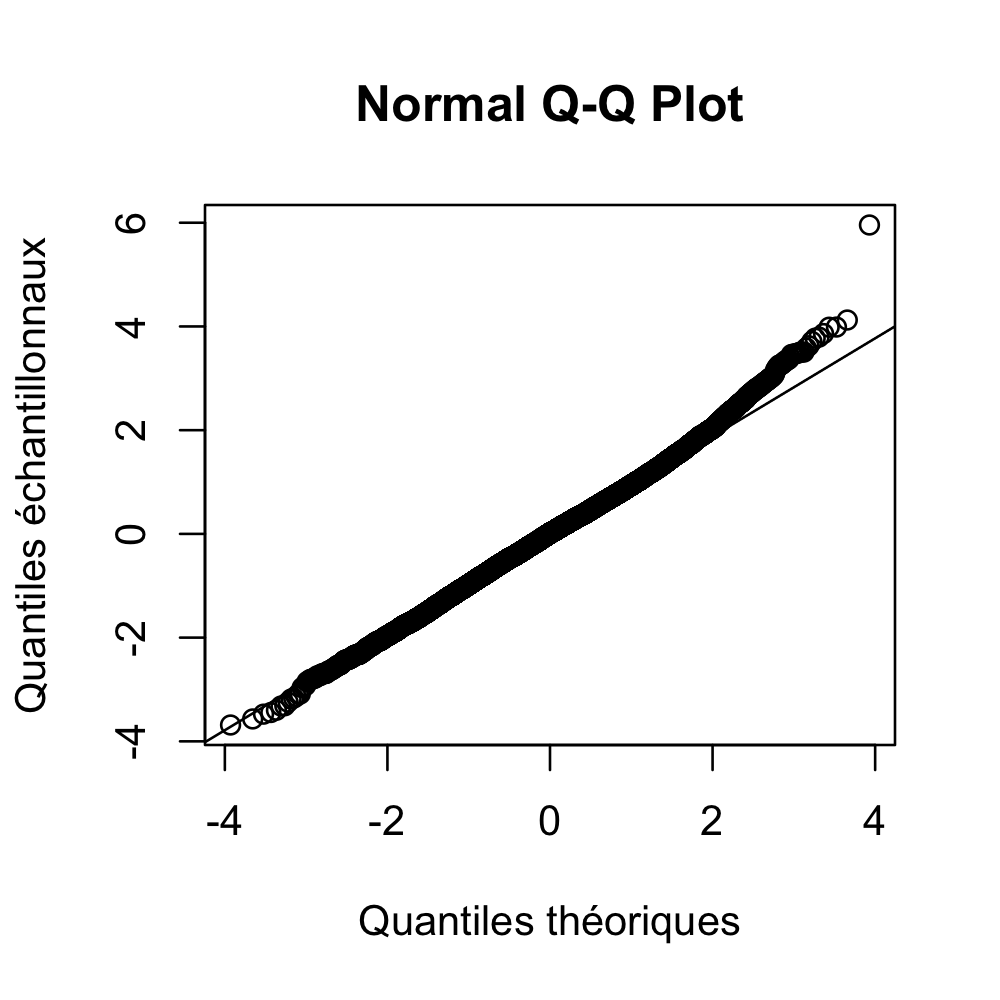
\includegraphics[width=5in]{figs/supp_figs/qq_plot_size.png}}{Figure \ref{fig:qqplot-size}}
    \caption{Graphique quantile-quantile des résidus du modèle de composition de taille calculés à l'aide de tirages MCCM à partir de la distribution postérieure des prédictions avec des effets fixes fixés aux estimations du maximum de vraisemblance et des effets aléatoires (c.-à-d., variance résiduelle) échantillonnés à partir de la distribution binomiale négative.}
    \label{fig:qqplot-size}
\end{figure}

\begin{figure}[htb]
    \centering
    \pdftooltip{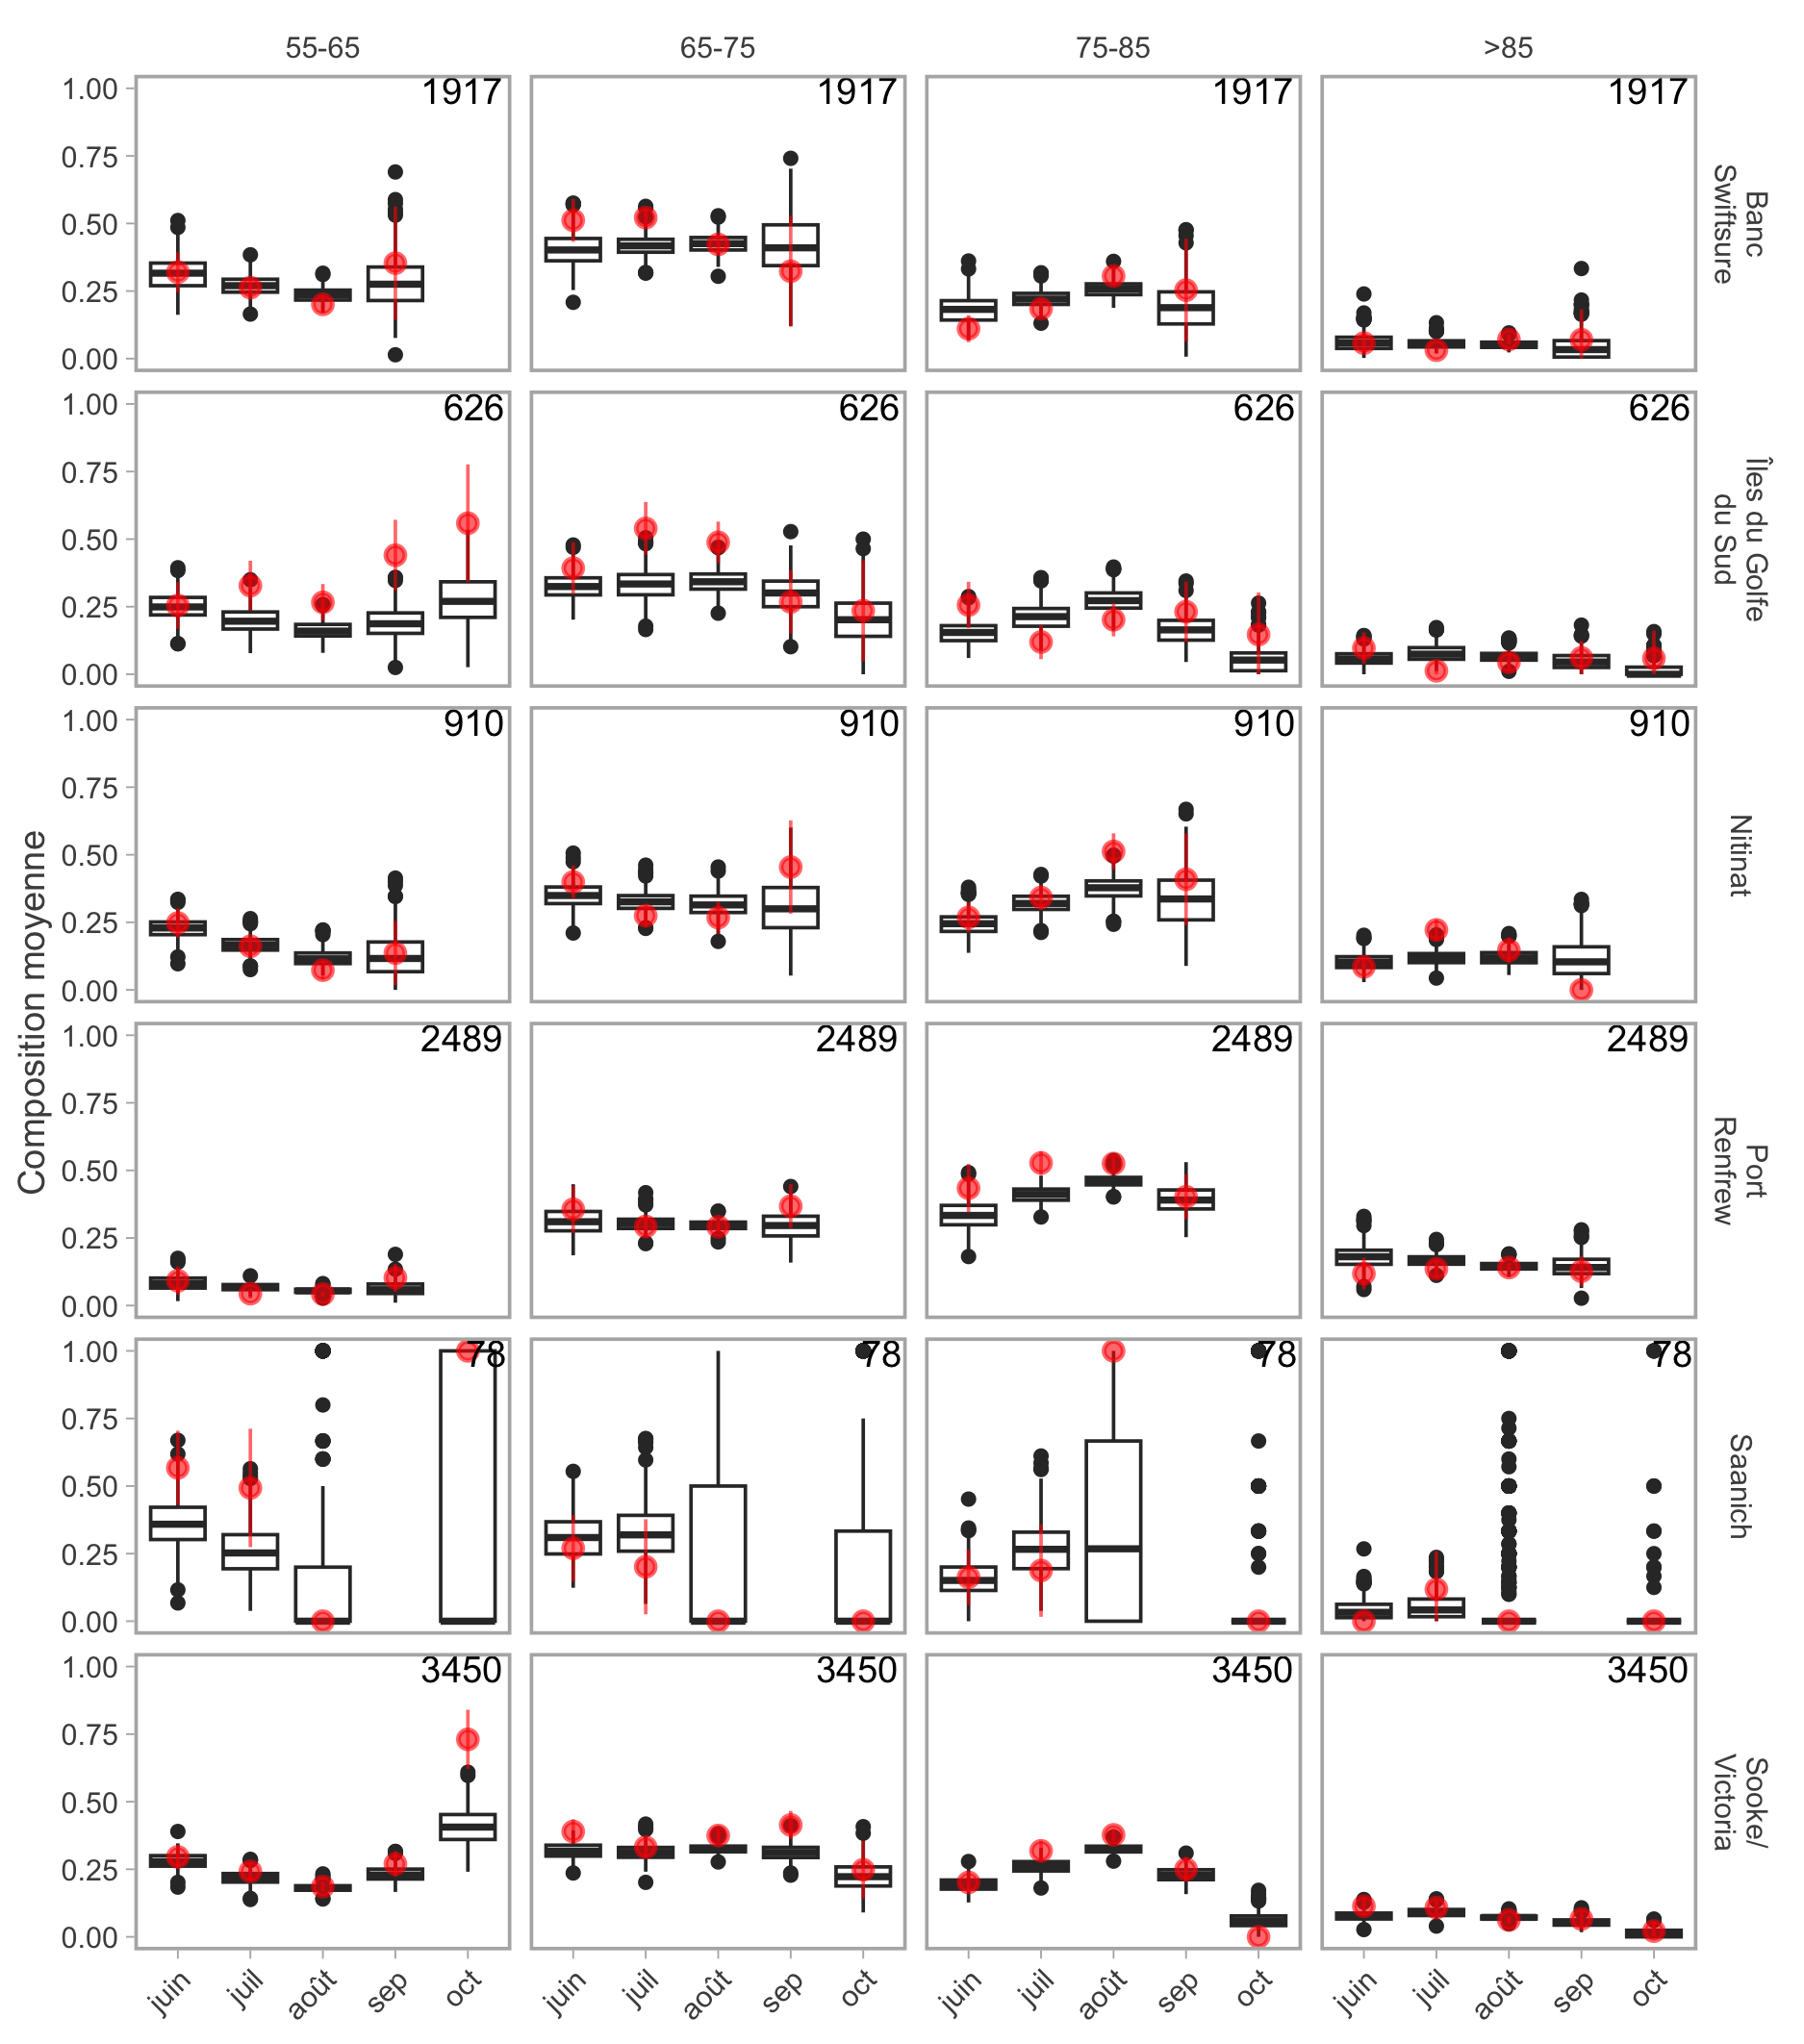
\includegraphics[width=5in]{figs/supp_figs/posterior_sims_size.png}}{Figure \ref{fig:posterior-size}}
    \caption{Composition moyenne simulée par modèle (diagrammes en boîte) et observée (points rouges) du stock. Les simulations représentent 500 tirages du modèle de Tweedie estimé, incluant la variance résiduelle, ajusté au jeu de données original. Les moustaches rouges représentent les intervalles de confiance approximatifs de 95\,\% associés à l'échantillon observé. Composition moyenne du stock calculée pour chaque strate et chaque mois. Les strates (panneaux) correspondent aux domaines spatiaux de la Figure \ref{fig:sampling-map}.}
    \label{fig:posterior-size}
\end{figure}

\clearpage

\renewcommand{\thechapter}{B}
\refstepcounter{chapter}
\starredchapter{ANNEXE~\thechapter. ESTIMATION DE LA TAILLE DES RESTES DE PROIES}\label{app:size-at-age}

Nous avons combiné les estimations de l'incertitude d'assignation de l'âge et la taille selon l'âge spécifique au stock pour convertir les estimations de l'âge marin des restes de proies des ERSN en estimations de la probabilité qu'un échantillon donné appartienne à une des quatre classes de taille.

\appsection{Incertitude d'assignation de l'âge}

Les restes de proies des ERSN ont été âgés en utilisant les annuli d'écailles par des techniciens du laboratoire de détermination de l'âge des poissons au laboratoire de sclérochronologie de la station biologique du Pacifique (Pêches et Océans Canada, Nanaimo, Colombie-Britannique, Canada). Les assignations d'âge basées sur les écailles sont couramment utilisées dans les évaluations de stock de saumon du Pacifique et l'exactitude est typiquement élevée \citep{mcnicolAccuracyUsingScales2010}; cependant, ces estimations peuvent dévier de l'âge véritable résultant en erreur. Nous avons d'abord estimé l'ampleur et la direction (c.-à-d., surestimation vs. sous-estimation) de l'erreur de détermination de l'âge en utilisant des données de saumon chinook avec à la fois un âge estimé à partir des lectures d'écailles, ainsi qu'un âge connu des étiquettes de fil codé ou des étiquettes basées sur la parenté. Nous avons ensuite ajusté un modèle hiérarchique pour estimer l'erreur de détermination de l'âge associée à un échantillon collecté à partir des restes de proies des ERSN.

Les données d'âge estimé et véritable étaient disponibles pour 16 528 saumons chinook. Ces données provenaient du jeu de données de la pêche récréative présenté dans le texte principal, ainsi que des données de l'Évaluation des stocks du Fraser et de l'intérieur, qui ont collecté des échantillons dans le cadre de pêches d'essai en eau douce et d'échantillonnage d'échappée. Bien que des échantillons étaient disponibles pour chacun des stocks inclus dans le texte principal, les tailles d'échantillon spécifiques au stock variaient largement (p. ex., deux échantillons pour Columbia River Spring, 4 508 pour Fraser River Fall). Nous n'avons pas tenu compte de l'incertitude d'assignation du stock dans cette analyse. Chaque échantillon a été assigné à une des trois catégories de biais : zéro (âges estimé et véritable étaient identiques), sous-estimation (âge véritable supérieur à l'âge estimé), ou surestimation (âge véritable inférieur à l'âge estimé). Nous avons exclu 48 échantillons où la différence entre les âges véritables et estimés était supérieure à une année. 

La directionalité des erreurs différait entre les âges estimés -- les poissons estimés être plus âgés que quatre ans étaient plus susceptibles d'être surestimés, tandis que ceux estimés être plus jeunes que quatre ans étaient plus susceptibles d'être sous-estimés (Figure \ref{fig:age-error-bar}). L'exactitude était aussi typiquement la plus élevée pour les classes d'âge dominantes dans un stock (Figure \ref{fig:age-error-bar}).

\begin{figure}[htb]
    \centering
    \pdftooltip{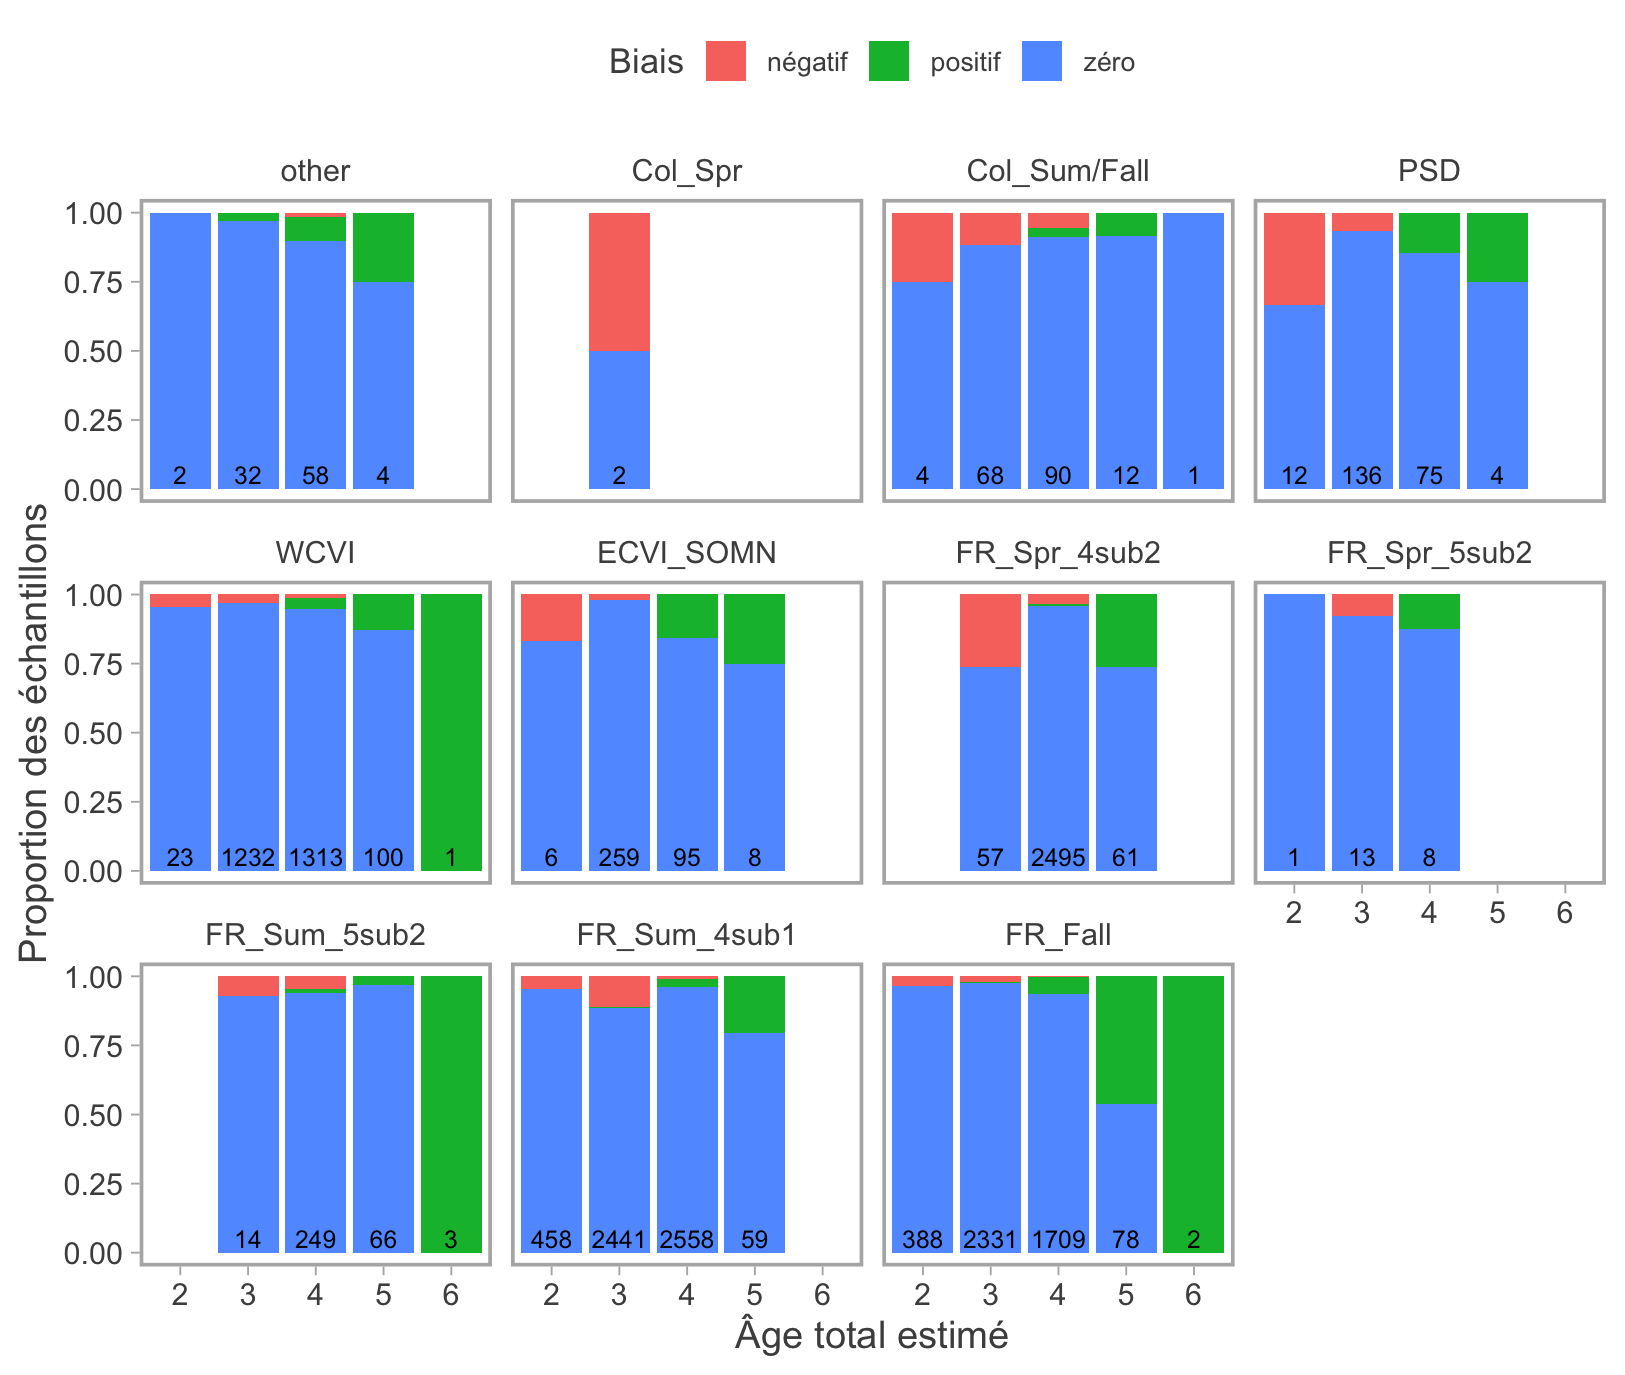
\includegraphics[width=5in]{figs/supp_figs/age_error.png}}{Figure \ref{fig:age-error-bar}}
    \caption{Biais dans l'âge total estimé parmi les stocks de saumon chinook. Les chiffres représentent le nombre d'échantillons dans une classe d'âge et un stock donnés.}
    \label{fig:age-error-bar}
\end{figure}

Pour générer des estimations d'erreur de détermination de l'âge pour les restes de proies des ERSN, nous avons ajusté un modèle multinomial hiérarchique dans lequel les trois catégories de biais (zéro, sous, ou sur) étaient la variable réponse, l'âge estimé était un effet fixe, et l'identité du stock était une interception aléatoire. Cette structure nous a permis de générer des taux d'erreur spécifiques à l'âge et au stock, tout en exploitant les stocks riches en données pour informer les stocks limités en données. Nous avons ajusté le modèle dans Stan via le paquet brms \citep{burknerBrmsPackageBayesian2017}, en utilisant des a priori faiblement informatifs. Nous avons utilisé le modèle ajusté pour convertir l'âge estimé associé à chaque échantillon de proie des ERSN en un vecteur de probabilités d'assignation de l'âge total $a_t$ $\boldsymbol{q_{a_t}}$, qui incorporait les taux d'erreur spécifiques à l'âge et au stock. Par exemple, un échantillon identifié comme provenant d'un individu Fraser Fall avec un âge total estimé de cinq ans pourrait résulter en une probabilité de 50\,\% d'être âgé de 4 ans et une probabilité de 50\,\% d'être âgé de 5 ans. 

\appsection{Estimations de taille selon l'âge}

Pour estimer la taille des proies à partir d'échantillons d'écailles, nous avons utilisé un modèle statistique pour prédire la taille selon l'âge en utilisant des données de la pêche récréative de saumon chinook. Ici, nous avons supposé qu'une probabilité d'assignation de stock supérieure à 75\,\% était exacte et avons exclu les échantillons en dessous de ce seuil. Les estimations d'âge marin, de taille corporelle et d'identité de stock étaient disponibles pour 7 815 saumons chinook plus grands que 550 mm de longueur à la fourche. Nous avons estimé la taille $b$ pour le stock $s$ en utilisant le modèle additif généralisé suivant :

\begin{align}
\label{eq:size_eq}
\tag{1}
b_{s} &\sim \operatorname{Normal} \left( \mu_{b_s}, \sigma^2 \right),\\
\tag{2}
\mu_{b_s} &= \alpha_s + \alpha_a + f_{w}w + f_{w_{s}}w + f_{w_{a}}w + \alpha_y \\
\notag
\end{align}
\noindent

Où $\alpha_a$ représente une interception pour l'âge marin $a$ et $\alpha_s$ représente une interception pour chaque stock. Nous avons représenté les changements saisonniers de taille corporelle avec $f_{w}$, une fonction lisse de processus gaussien pour la semaine d'échantillonnage $w$. Nous avons aussi permis à la variabilité saisonnière de différer entre les stocks et les classes d'âge marin, en utilisant des lissages hiérarchiques $f_{w_s}$ et $f_{w_a}$. Finalement, nous avons inclus une interception aléatoire $\alpha_y$ représentant les changements spécifiques à l'année dans la taille moyenne. Nous avons modélisé $\alpha_y$ en supposant une hyperdistribution avec une moyenne zéro et un écart-type $\sigma_y$. Notez que les groupements de stocks utilisés dans le modèle de taille selon l'âge étaient plus finement résolus que ceux utilisés dans les analyses de composition de stock pour augmenter la précision des prédictions.

Nous avons utilisé le modèle ajusté pour visualiser les motifs saisonniers dans la taille selon l'âge spécifique au stock et prédire la taille moyenne de chaque échantillon de proie des ERSN qui avait une estimation d'âge viable basée sur l'identité du stock associé et la semaine d'échantillonnage. Nous n'avons pas généré de prédictions spécifiques à l'année (c.-à-d., intégré hors $\alpha_y$) étant donné que de nombreux échantillons ont été collectés avant l'échantillonnage de la pêche récréative. 

Les stocks de saumon chinook capturés dans la zone d'étude différaient en âge marin, mais généralement les individus d'âge marin 2 et 3 étaient les plus communs (Figure \ref{fig:rec-age-comp}). Notez que ces observations sous-représenteront les individus d'âge marin 1 et 2 (particulièrement pour les histoires de vie de juvéniles de l'année) parce qu'ils excluent les individus plus petits que 550 mm de longueur à la fourche pour rester cohérent avec le reste de l'analyse.

\begin{figure}[htb]
    \centering
    \pdftooltip{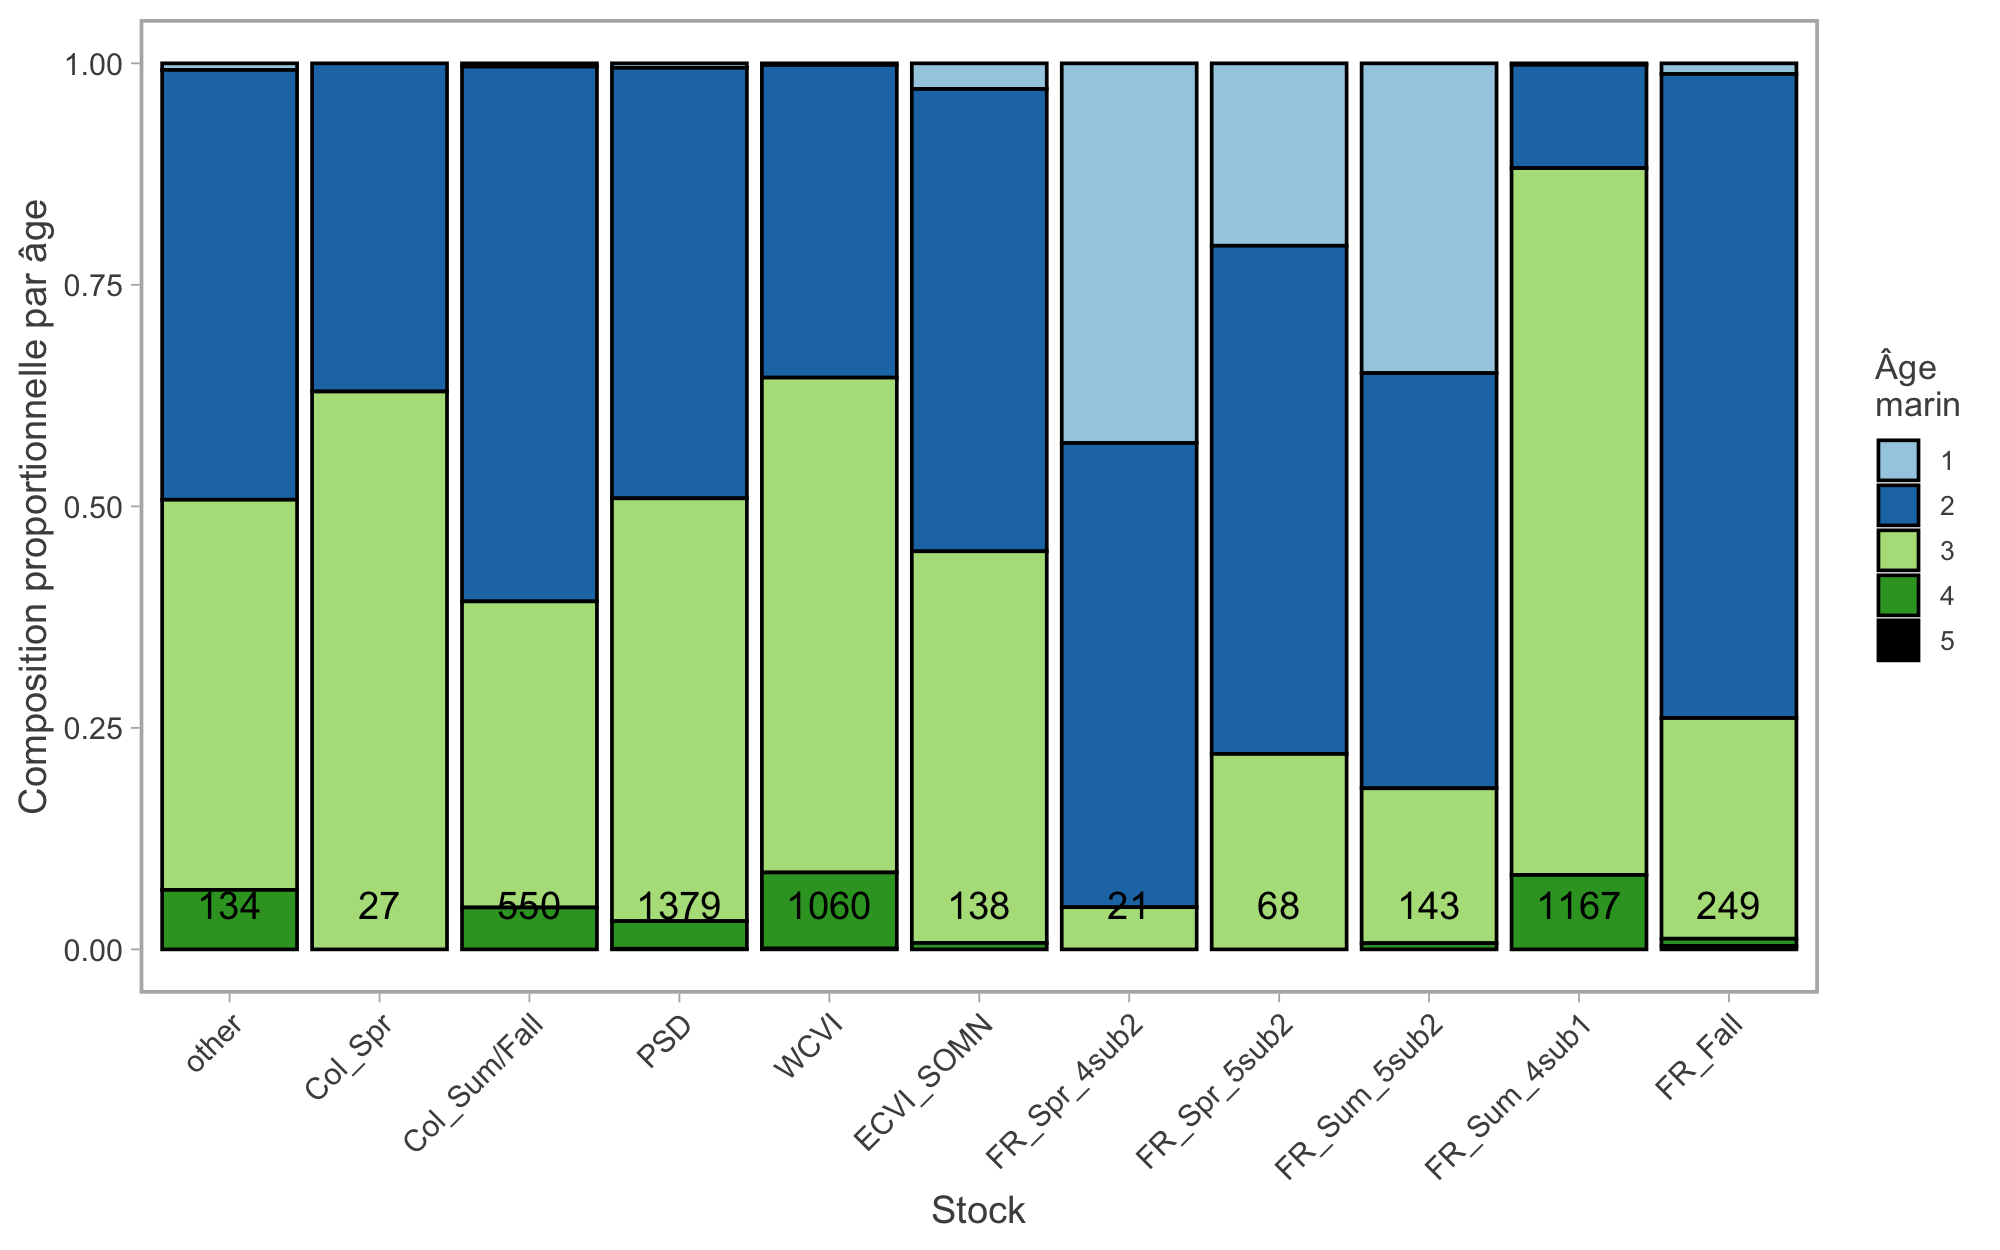
\includegraphics[width=5in]{figs/supp_figs/comp_bar_fishery_age_sw.png}}{Figure \ref{fig:rec-age-comp}}
    \caption{Âge marin observé du saumon chinook des pêches récréatives du sud de la C.-B.}
    \label{fig:rec-age-comp}
\end{figure}

Les âges marins plus vieux étaient plus grands que les âges marins plus jeunes et les stocks variaient en taille selon l'âge, avec les stocks de juvéniles d'un an typiquement plus grands à l'âge marin 2 que les stocks de juvéniles de l'année (Figure \ref{fig:pred-size-at-age}). Le saumon chinook a montré des preuves de changements dans la taille corporelle au cours de l'été; cependant, ces tendances différaient entre les stocks et entre les classes d'âge marin. Le modèle a capturé avec précision la variabilité de taille à l'intérieur des classes d'âge, ce qui a résulté en des distributions de taille qui se chevauchent (Figure \ref{fig:hist-size-at-age}). 

\begin{figure}[htb]
    \centering
    \pdftooltip{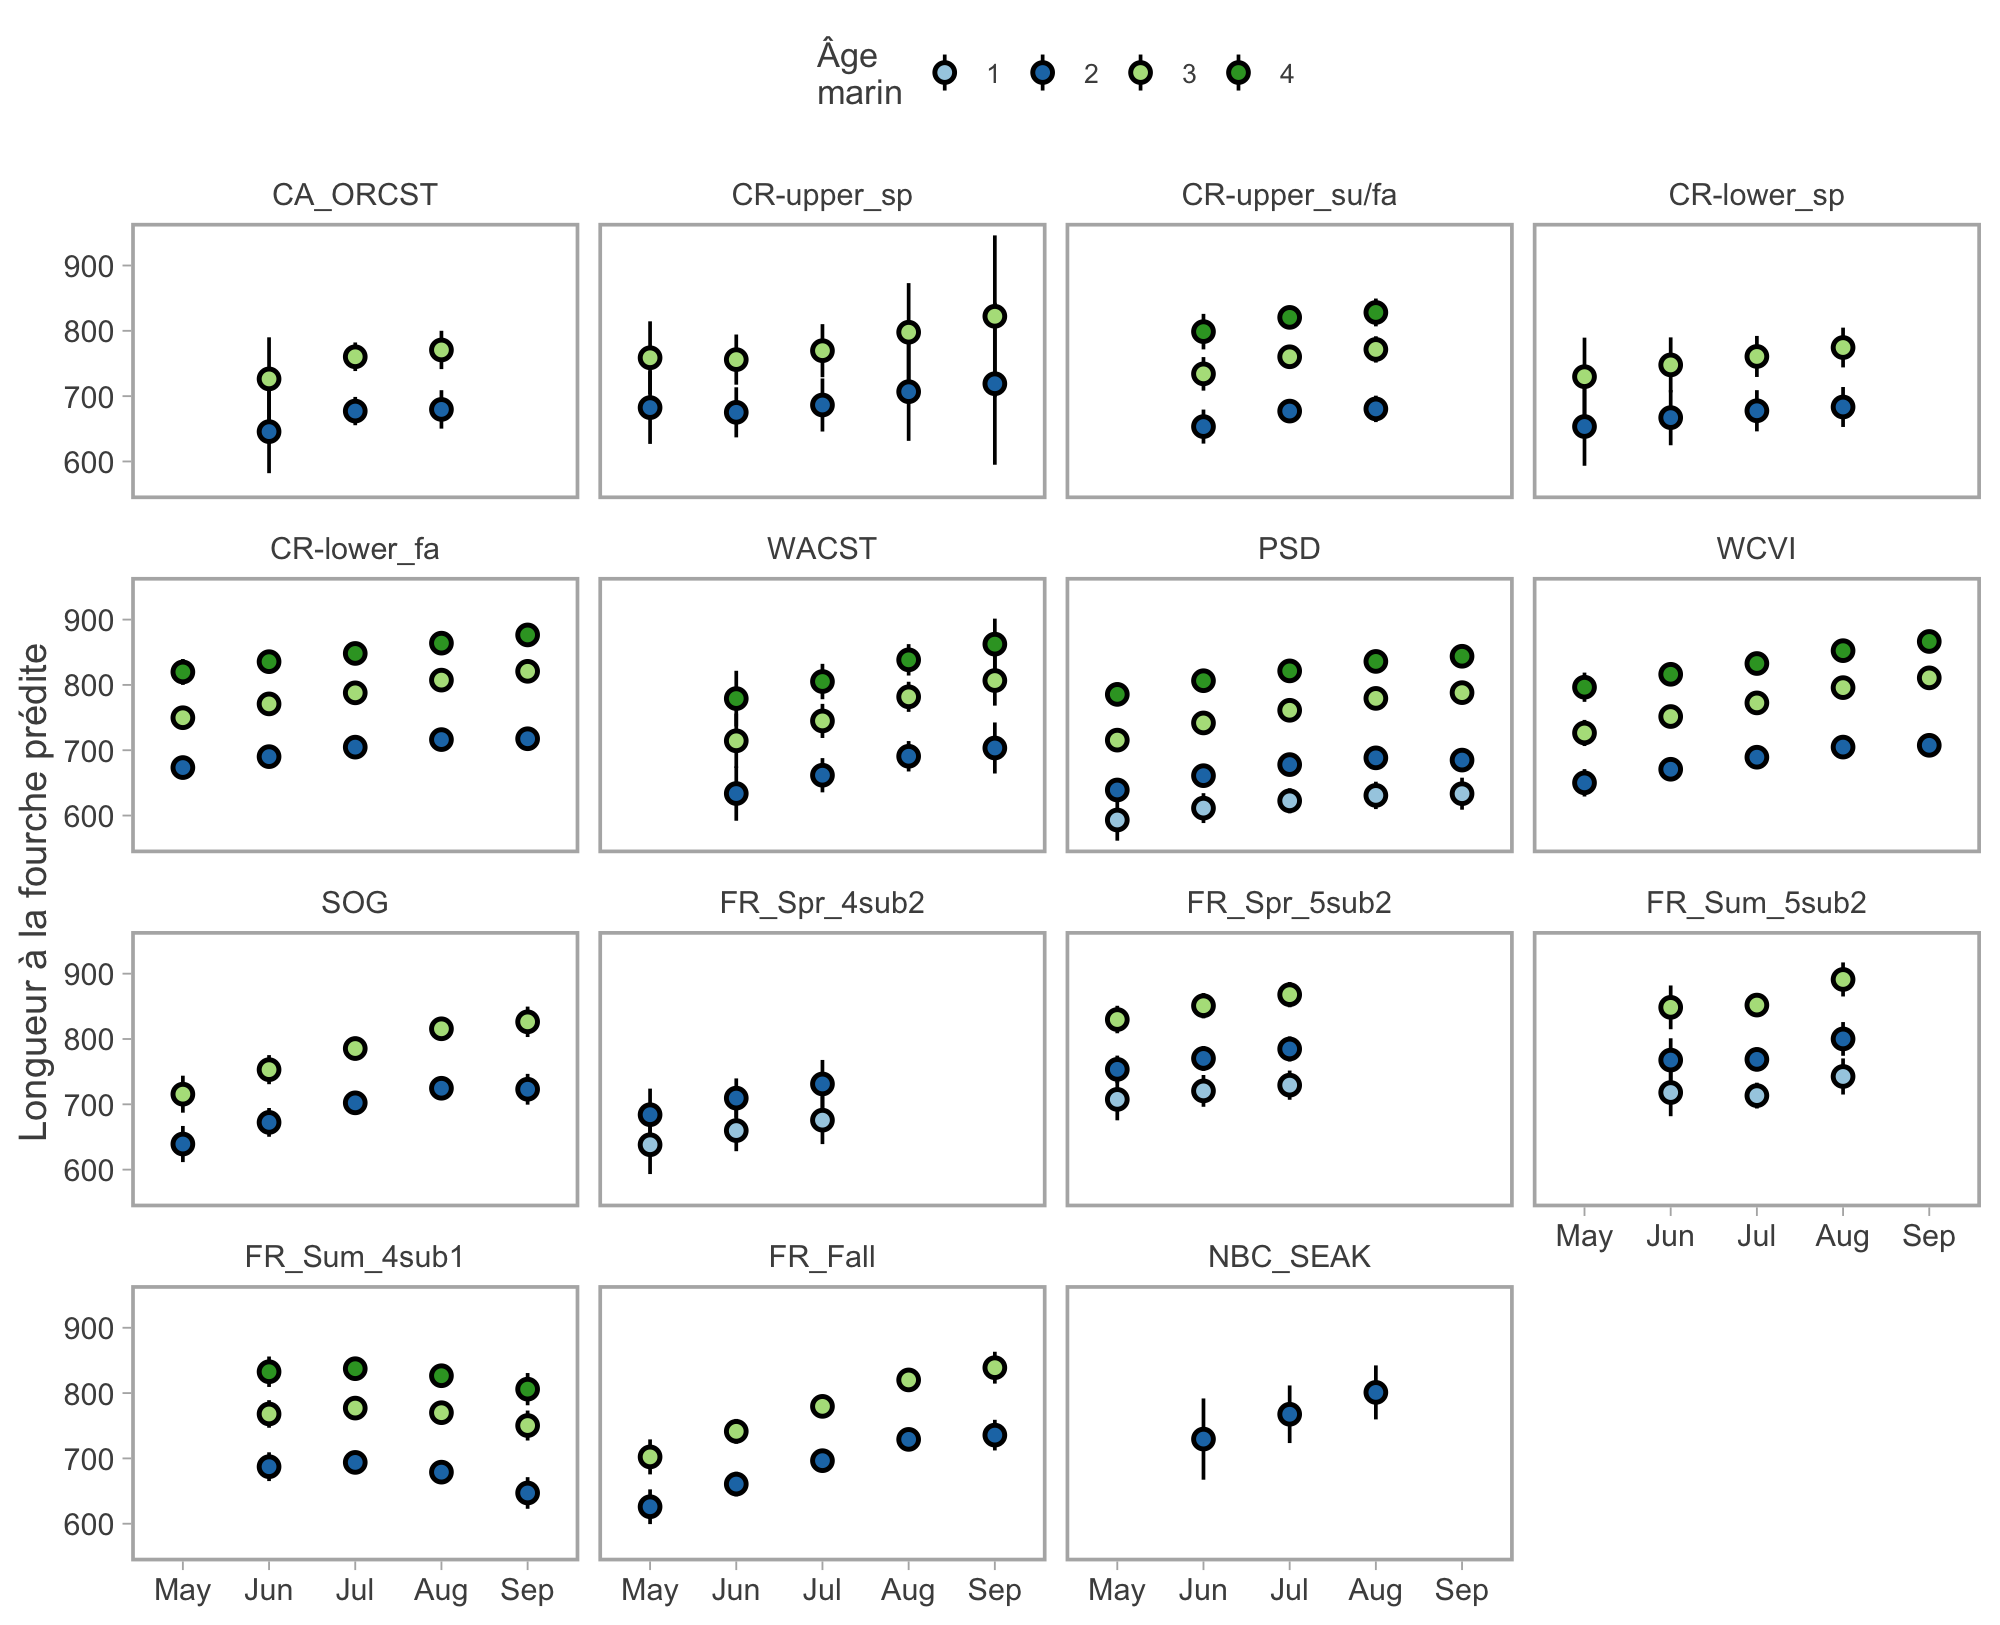
\includegraphics[width=5in]{figs/supp_figs/mean_pred_fishery.png}}{Figure \ref{fig:pred-size-at-age}}
    \caption{Taille selon l'âge prédite par le modèle. Les points représentent les moyennes et les moustaches les intervalles de confiance à 95\,\%. Les prédictions ne sont montrées que pour les mois et âges marins où au moins cinq individus du stock pertinent étaient disponibles pour paramétrer le modèle.}
    \label{fig:pred-size-at-age}
\end{figure}

\begin{figure}[htb]
    \centering
    \pdftooltip{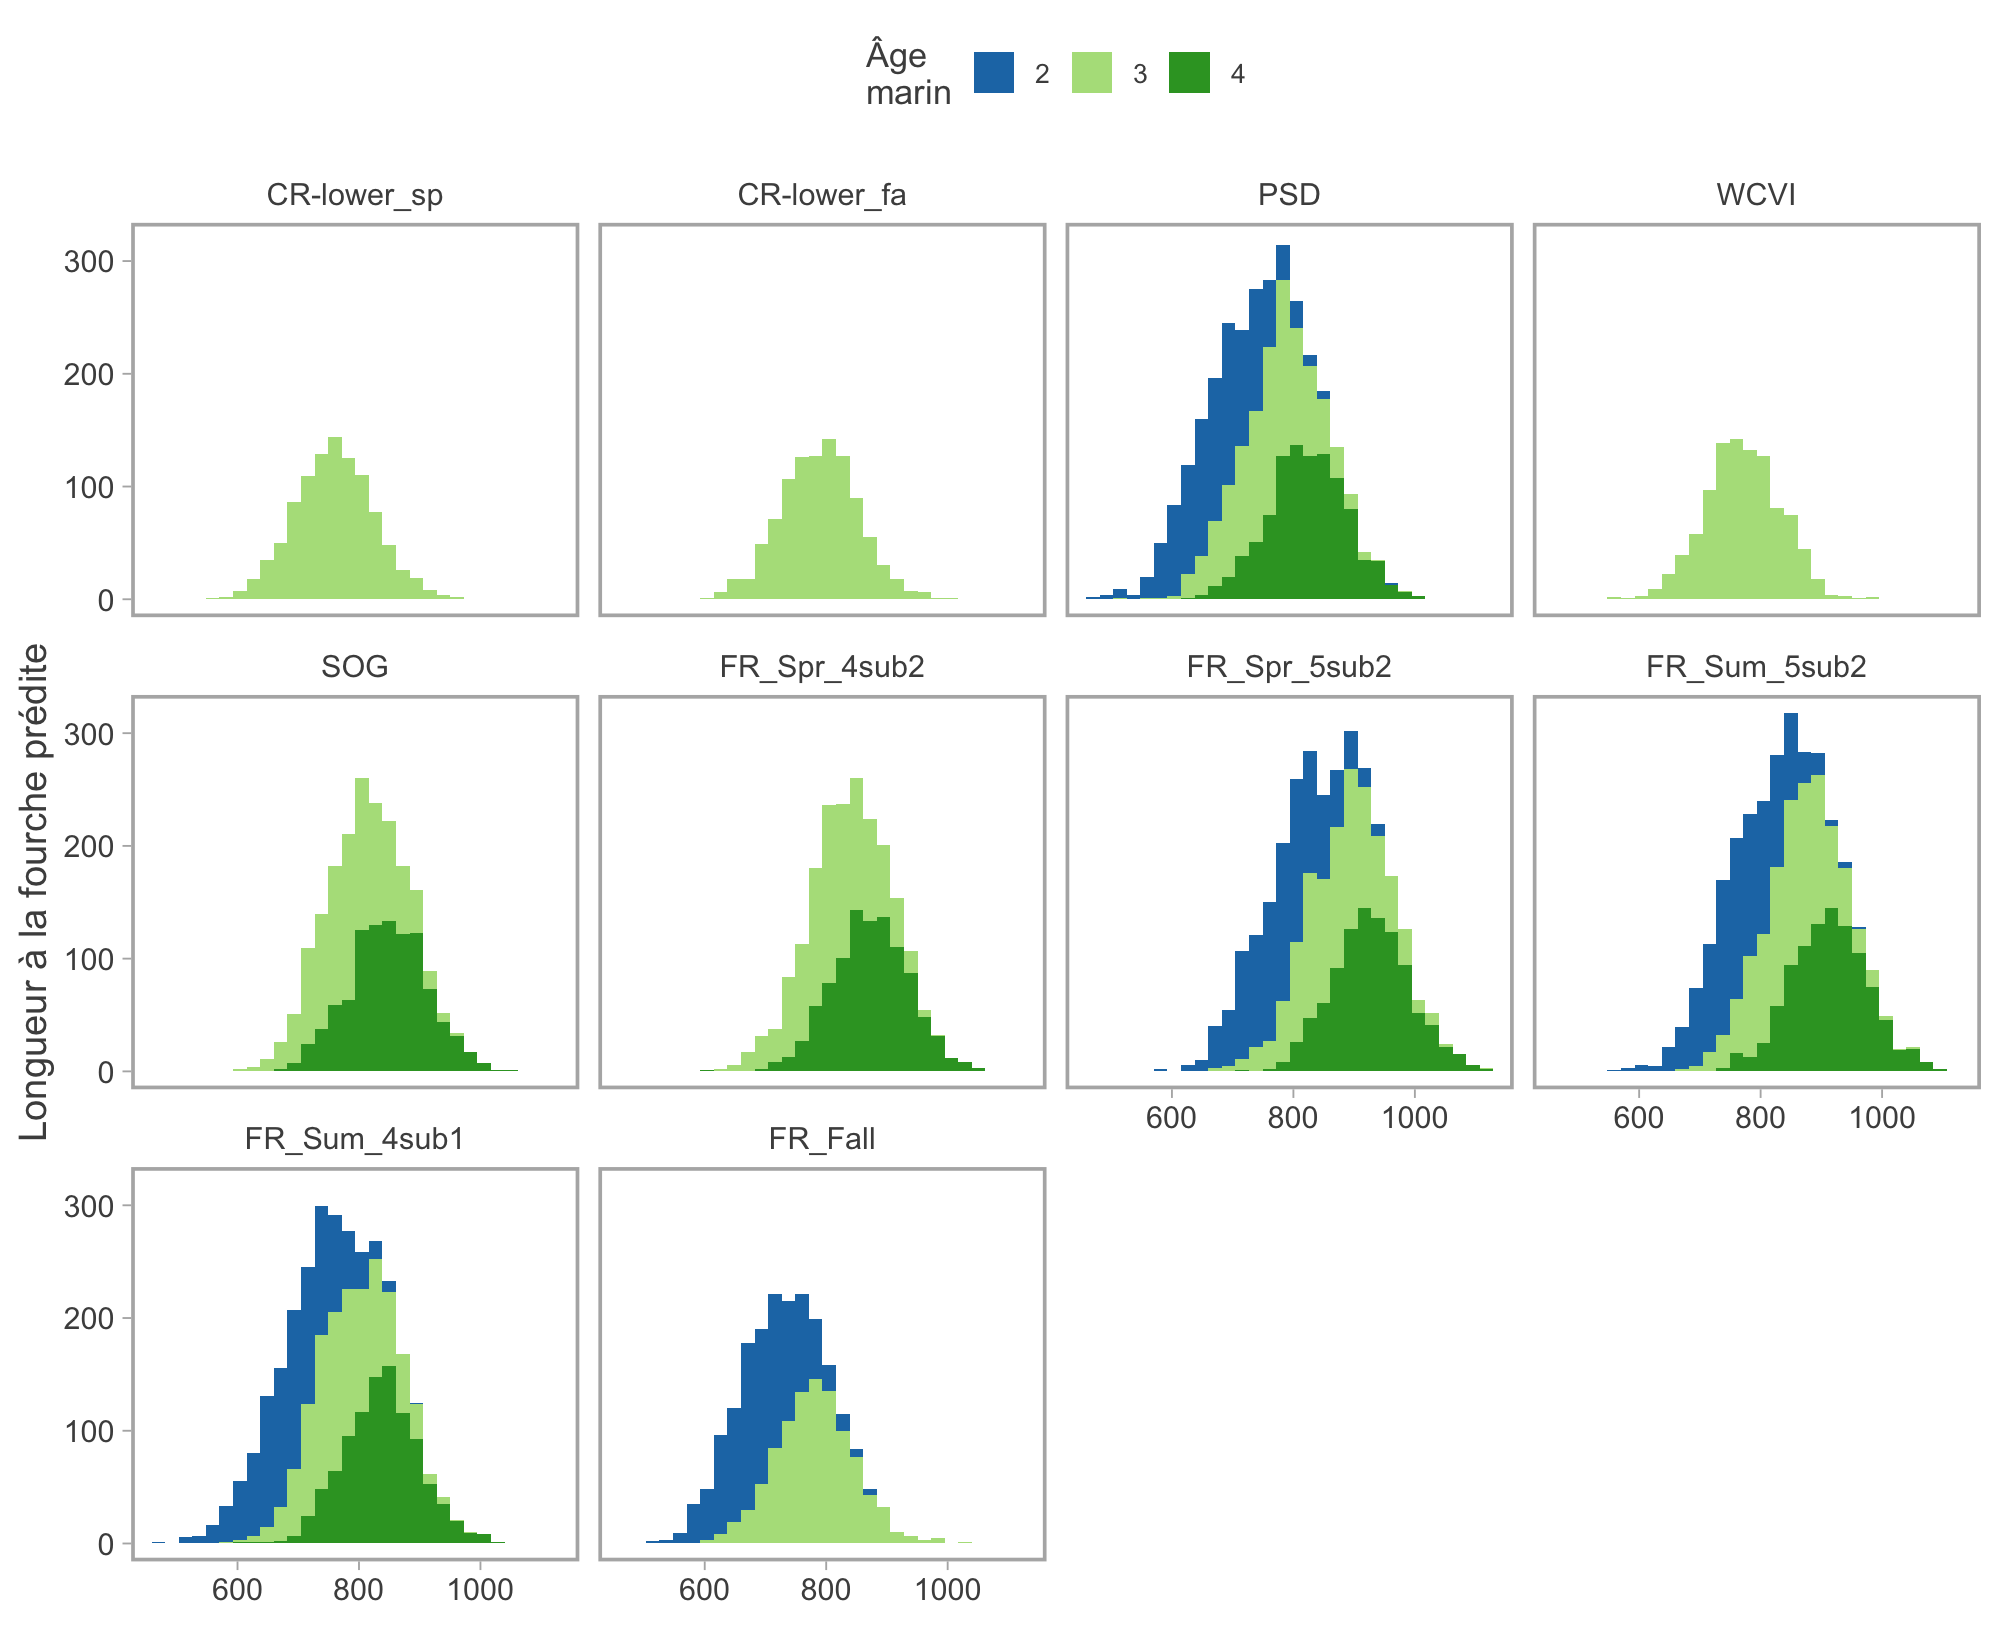
\includegraphics[width=5in]{figs/supp_figs/hist_pred_fishery.png}}{Figure \ref{fig:hist-size-at-age}}
    \caption{Distributions de taille selon l'âge prédites par le modèle pour juillet. Les distributions ont les mêmes moyennes que la Figure \ref{fig:pred-size-at-age}, mais incorporent la variabilité résiduelle autour de la moyenne. Seules les combinaisons d'âge et de stock observées dans les restes de proies des ERSN sont montrées.}
    \label{fig:hist-size-at-age}
\end{figure}

Nous avons utilisé le modèle ajusté pour générer une distribution postérieure de 1 000 échantillons de taille corporelle pour chaque combinaison de stock, d'âge marin et de mois observée dans les restes de proies des ERSN.

\appsection{Propagation de l'incertitude aux estimations de taille des restes de proies des ERSN}

Nous avons utilisé un processus en plusieurs étapes pour identifier un vecteur de probabilités qu'un échantillon donné de restes de proies des ERSN appartienne à une des quatre classes de taille $b'$. Premièrement, nous avons converti le vecteur de probabilités d'âge total $\boldsymbol{q_{a_t}}$ en un vecteur de probabilités d'âge marin $\boldsymbol{q_{a}}$, basé sur l'âge marin de l'échantillon lorsqu'une estimation était disponible ou basé sur l'histoire de vie dominante d'un stock autrement. Deuxièmement, pour chaque échantillon, nous avons tiré des distributions postérieures précédemment décrites d'estimations de taille corporelle spécifiques au stock, à l'âge marin et au mois proportionnellement à $\boldsymbol{q_{a}}$. En supposant que l'exemple précédemment décrit a été collecté en juin et appartenait à un individu Fraser Fall avec une probabilité de 50\,\% d'être âgé de 4 ans et une probabilité de 50\,\% d'être âgé de 5 ans, alors nous tirerions 500 échantillons de la distribution de taille Fraser Fall de juin âgé de 4 ans et 500 échantillons de la distribution de taille Fraser Fall de juin âgé de 5 ans (p. ex., Figures \ref{fig:pred-size-at-age}, \ref{fig:hist-size-at-age}). Troisièmement, nous avons converti chaque échantillon de taille en une classe de taille $b'$ et avons calculé la proportion des 1 000 échantillons appartenant à chaque classe, créant un vecteur de probabilités de classe de taille $q_{b'}$ pour chaque échantillon. 

Pour s'assurer que cette analyse était traitable, nous n'avons pas propagé l'incertitude d'assignation du stock. Au lieu de cela, nous avons utilisé la probabilité d'assignation de stock maximale pour chaque échantillon individuel pour générer $q_{b'}$. Nous croyons que cette supposition est peu susceptible d'impacter fortement nos résultats étant donné : des biais d'âge similaires entre les stocks, des distributions de taille selon l'âge largement chevauchantes entre les stocks (Figure \ref{fig:hist-size-at-age}), les échantillons de proies avec une probabilité d'assignation inférieure à 60\,\% ont été exclus, et qu'environ 90\,\% des échantillons inclus avaient une probabilité d'assignation supérieure à 80\,\%.
\clearpage

\renewcommand{\thechapter}{C}
\refstepcounter{chapter}
\starredchapter{ANNEXE~\thechapter. ABONDANCE TERMINALE}\label{app:terminal-abundance}

Nous avons rassemblé les données sur l'abondance terminale pour les stocks américains du jeu de données historique du Conseil de gestion des pêches du Pacifique des échappées vers les pêches continentales et les zones de frai \citep{pfmcEscapementsInlandFisheries2024}. Les données d'abondance terminale pour les stocks canadiens provenaient des bureaux d'évaluation des stocks de zone du MPO (Tableau \ref{tab:sources}).  

\begin{table}[h!]
\centering
\begin{threeparttable}
\caption{Définitions et sources de l'abondance terminale par stock.}
\label{tab:sources}
\begin{tabular}{p{5cm}p{4.5cm}p{4.5cm}}
\toprule
\textbf{Stock} & \textbf{Données incluses} & \textbf{Source} \\
\midrule
Côtière de Washington et de l'Oregon\tnote{1} & Prises terminales plus échappée\tnote{2} & \cite{pfmcEscapementsInlandFisheries2024} \\
Columbia River Summer/Fall & Prises en rivière plus échappée & \cite{pfmcEscapementsInlandFisheries2024} \\
Côte ouest de l'île de Vancouver & Prises à l'intérieur de la ligne de ressac (c.-à-d., ZGPF 23-27) et en rivière plus échappée & Évaluation des stocks de la côte sud du MPO; Nick Brown, comm. pers. \\
Côte est de l'île de Vancouver/baies du continent méridional & Échappée & Évaluation des stocks de la côte sud du MPO; Kevin Pellett, comm. pers. \\
Puget Sound & Échappée plus prises terminales & \cite{pfmcEscapementsInlandFisheries2024} \\
Fraser River Spring 42 & Prises en rivière plus échappée & MPO 2024; Brittany Jenewein, comm. pers. \\
Fraser River Spring 52 & Prises en rivière plus échappée & MPO 2024; Brittany Jenewein, comm. pers. \\
Fraser River Summer 52 & Prises en rivière plus échappée & MPO 2024; Brittany Jenewein, comm. pers. \\
Fraser River Summer 41 & Prises en rivière plus échappée & MPO 2024; Brittany Jenewein, comm. pers. \\
Fraser River Fall & Prises en rivière plus échappée & MPO 2024; Brittany Jenewein, comm. pers. \\
\bottomrule
\end{tabular}

\begin{tablenotes}
\item[1] Stocks côtiers de Washington et de l'Oregon groupés avec le stock «\,Autre\,» dans le texte principal.
\item[2] L'échappée inclut les géniteurs naturels, la capture de stock géniteur et les entrées nageantes aux installations d'écloserie pour tous les stocks.
\end{tablenotes}

\end{threeparttable}
\end{table}

Les estimations d'abondance terminale au niveau du stock sont basées sur les prises et l'échappée surveillées aux systèmes indicateurs, qui sont ensuite additionnées. Nous avons exclu les systèmes indicateurs avec une surveillance incomplète entre 1983 et 2022 pour éviter le biais temporel dû aux changements dans l'échantillonnage. Ainsi, les estimations d'abondance terminale devraient être interprétées comme des estimations minimales d'abondance, particulièrement étant donné que dans certains stocks, seulement un sous-ensemble de tronçons sont surveillés. Pour les stocks côtiers de Washington et de Puget Sound, les données de 2023 n'étaient pas disponibles et ont été interpolées en utilisant les valeurs moyennes 2019-2022 (moyenne de ligne de cycle). Pour la côte est de l'île de Vancouver et les baies du continent méridional, les données au niveau du stock ont été générées en interpolant les estimations pour les systèmes indicateurs faiblement observés basées sur l'abondance proportionnelle moyenne des systèmes régulièrement surveillés (p. ex., rivière Cowichan) dans les années où tous les systèmes ont été observés. Finalement, nous avons exclu les estimations d'abondance terminale collectées avant 1982 en raison du relativement peu de séries temporelles complètes. 
\clearpage

\renewcommand{\thechapter}{D}
\refstepcounter{chapter}
\starredchapter{ANNEXE~\thechapter. ANALYSES DE SENSIBILITÉ}\label{app:sensitivity}

\appsection{Sélectivité de taille}

Nous avons tenu compte de la sélectivité de taille des ERSN en excluant les échantillons de la pêche récréative qui étaient plus petits que 75 cm de longueur à la fourche (>70\,\% des échantillons de régime alimentaire étaient estimés être supérieurs à cette taille) et en rajustant le modèle présenté dans le texte principal (Équation \ref{eq:comp_eq}). Notez que la simulation de composition de taille présentée dans le texte principal teste explicitement la sélectivité de taille. L'analyse présentée ici n'a été utilisée que pour évaluer l'interaction entre la taille et la sélectivité du stock.

Nous avons généré des prédictions (effets marginaux) de la composition saisonnière du stock à travers les strates et avons comparé qualitativement ces prédictions aux prédictions du modèle du texte principal. Nous avons également évalué l'effet de l'analyse de sensibilité sur la simulation de sélectivité du stock, en utilisant un modèle ajusté uniquement aux échantillons collectés de poissons plus grands que 75 cm de longueur à la fourche pour générer des vecteurs alternatifs de composition moyenne du stock ($\hat{\pi_{s_{size}}}$). 

Nous notons que cette analyse de sensibilité n'est pas une évaluation compréhensive du biais d'échantillonnage. Par exemple, le comportement de la flotte récréative a été impacté par une gamme de mesures de gestion qui changent saisonnièrement, spatialement et entre les années \citep{dobsonTechnicalReviewManagement2020, dfoPacificRegionFinal2023}. De même, les restes de proies peuvent être plus susceptibles d'être collectés de stocks de saumon chinook ayant des comportements particuliers. Bien qu'il n'ait pas été possible de tenir compte statistiquement de ces facteurs de confusion, nous explorons leurs impacts potentiels dans la Discussion du texte principal. 

Généralement, les motifs saisonniers dans la composition du stock étaient similaires, peu importe si les modèles étaient ajustés au jeu de données complet (texte principal) ou à un jeu contraint aux grands individus seulement. Cependant, il y avait des différences subtiles pour des stocks, des strates et des périodes spécifiques. Par exemple, les stocks «\,Autre\,», Puget Sound et ECVI/SOMN étaient relativement moins abondants dans des strates spécifiques lorsque les petits individus étaient exclus (Figures \ref{fig:comb-pred-stock1}, \ref{fig:comb-pred-stock2}). Inversement, les stocks du fleuve Fraser, excluant les individus Spring $4_2$, étaient typiquement plus abondants lorsque les petits individus étaient exclus (Figure \ref{fig:comb-pred-stock2}). 

\begin{figure}[H]
    \centering
    \pdftooltip{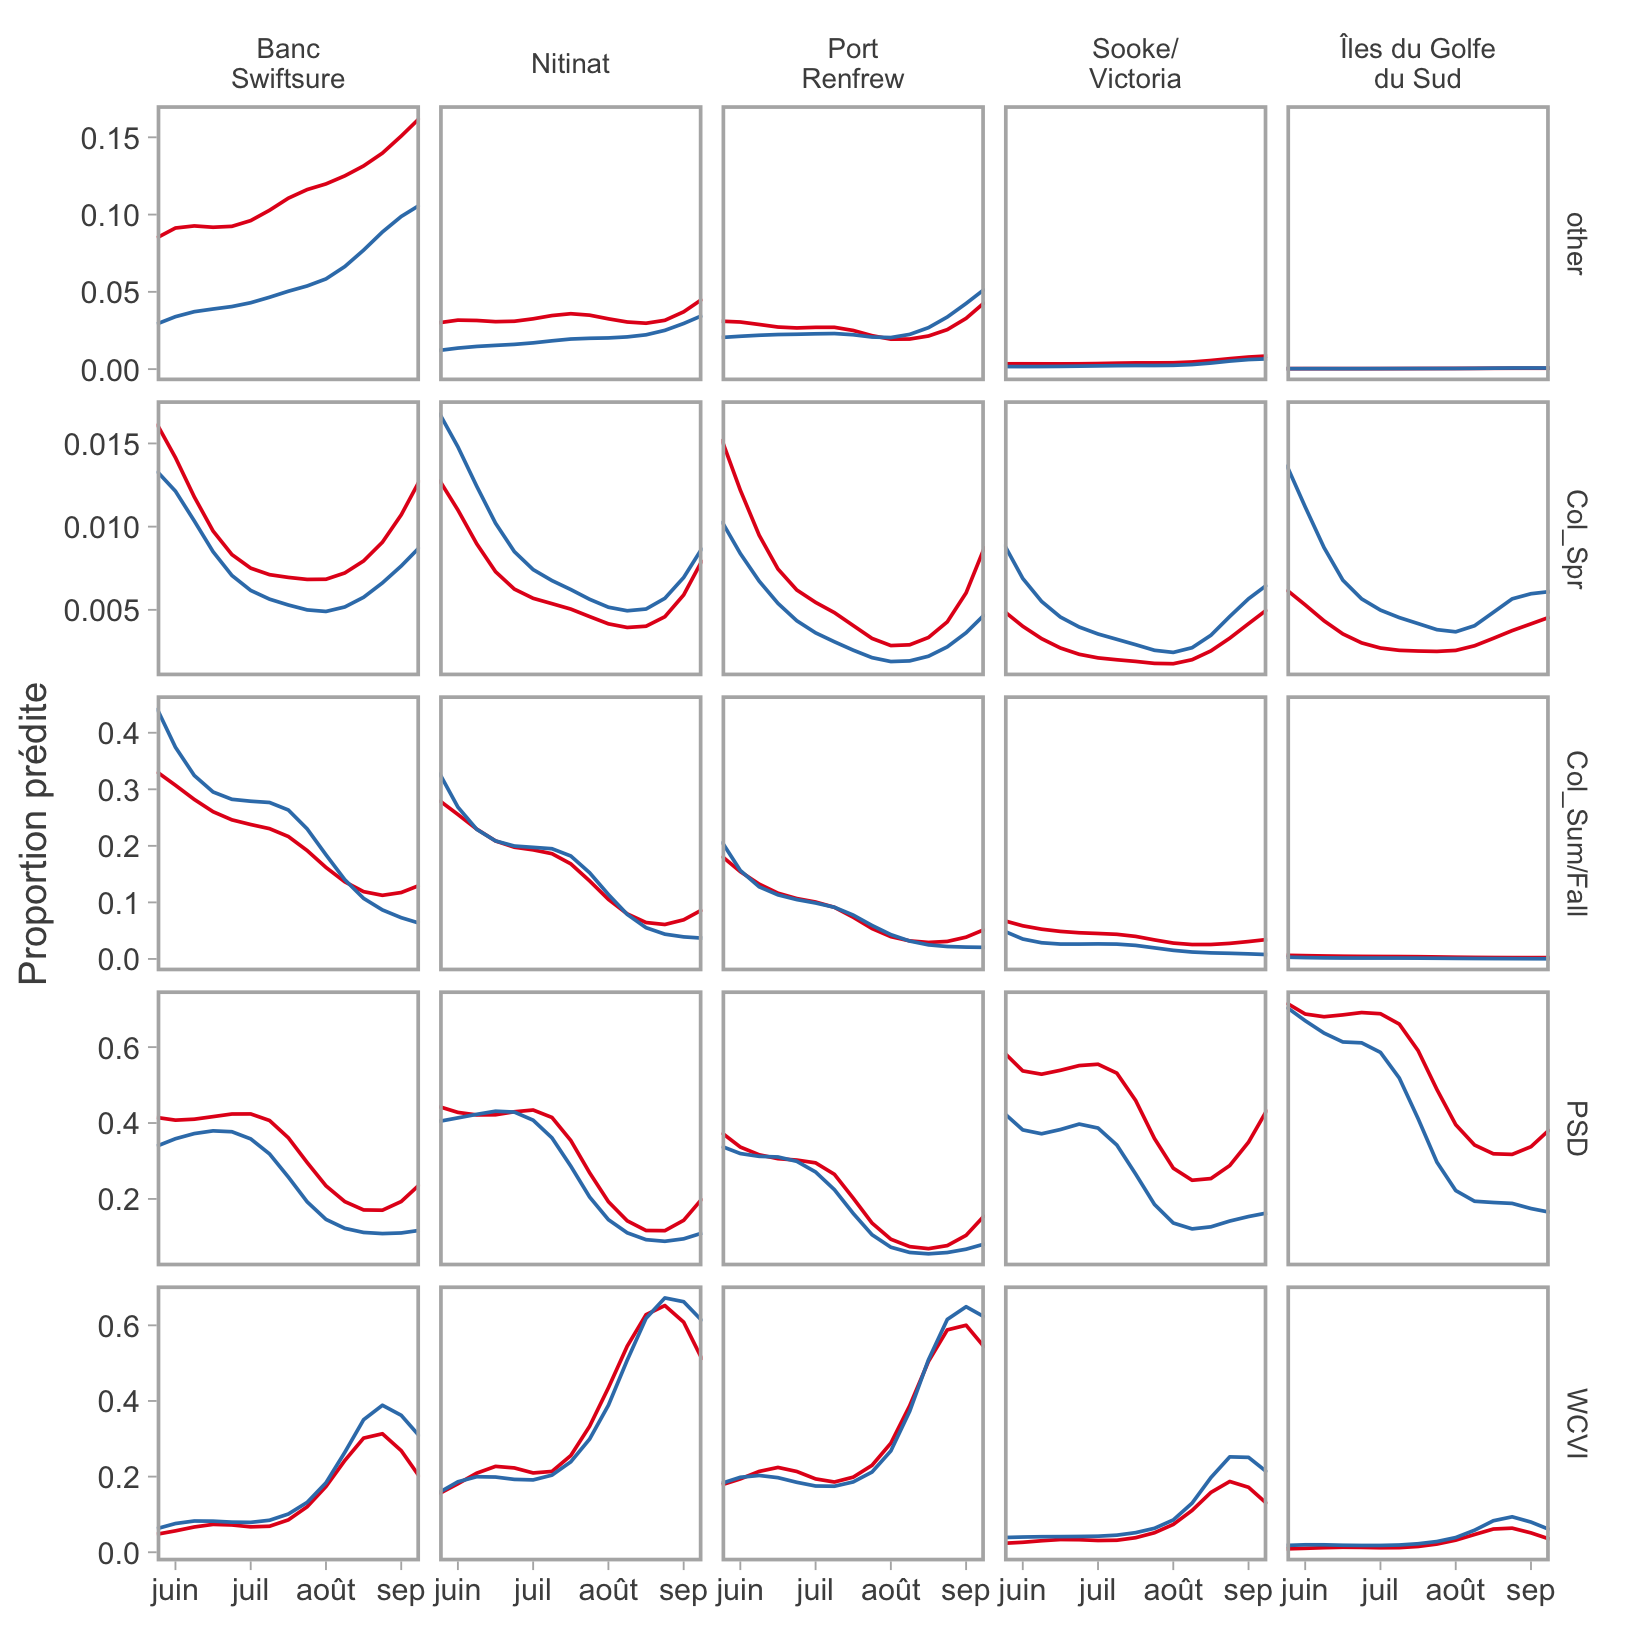
\includegraphics[width=5in]{figs/supp_figs/model_comp_stock1.png}}{Figure \ref{fig:comb-pred-stock1}}
    \caption{Prédictions saisonnières de l'abondance spécifique au stock pour les stocks autre, Columbia Spring, Columbia Summer/Fall, Puget Sound et côte ouest de l'île de Vancouver. Les prédictions sont basées sur le modèle standard présenté dans le texte principal (rouge), ainsi qu'un modèle ajusté uniquement aux données d'individus plus grands que 75 cm (bleu). Les prédictions représentent les estimations moyennes et les intervalles de confiance ne sont pas montrés pour améliorer la lisibilité. Notez les différences d'échelle de l'axe des y entre les stocks.}
    \label{fig:comb-pred-stock1}
\end{figure}

\begin{figure}[H]
    \centering
    \pdftooltip{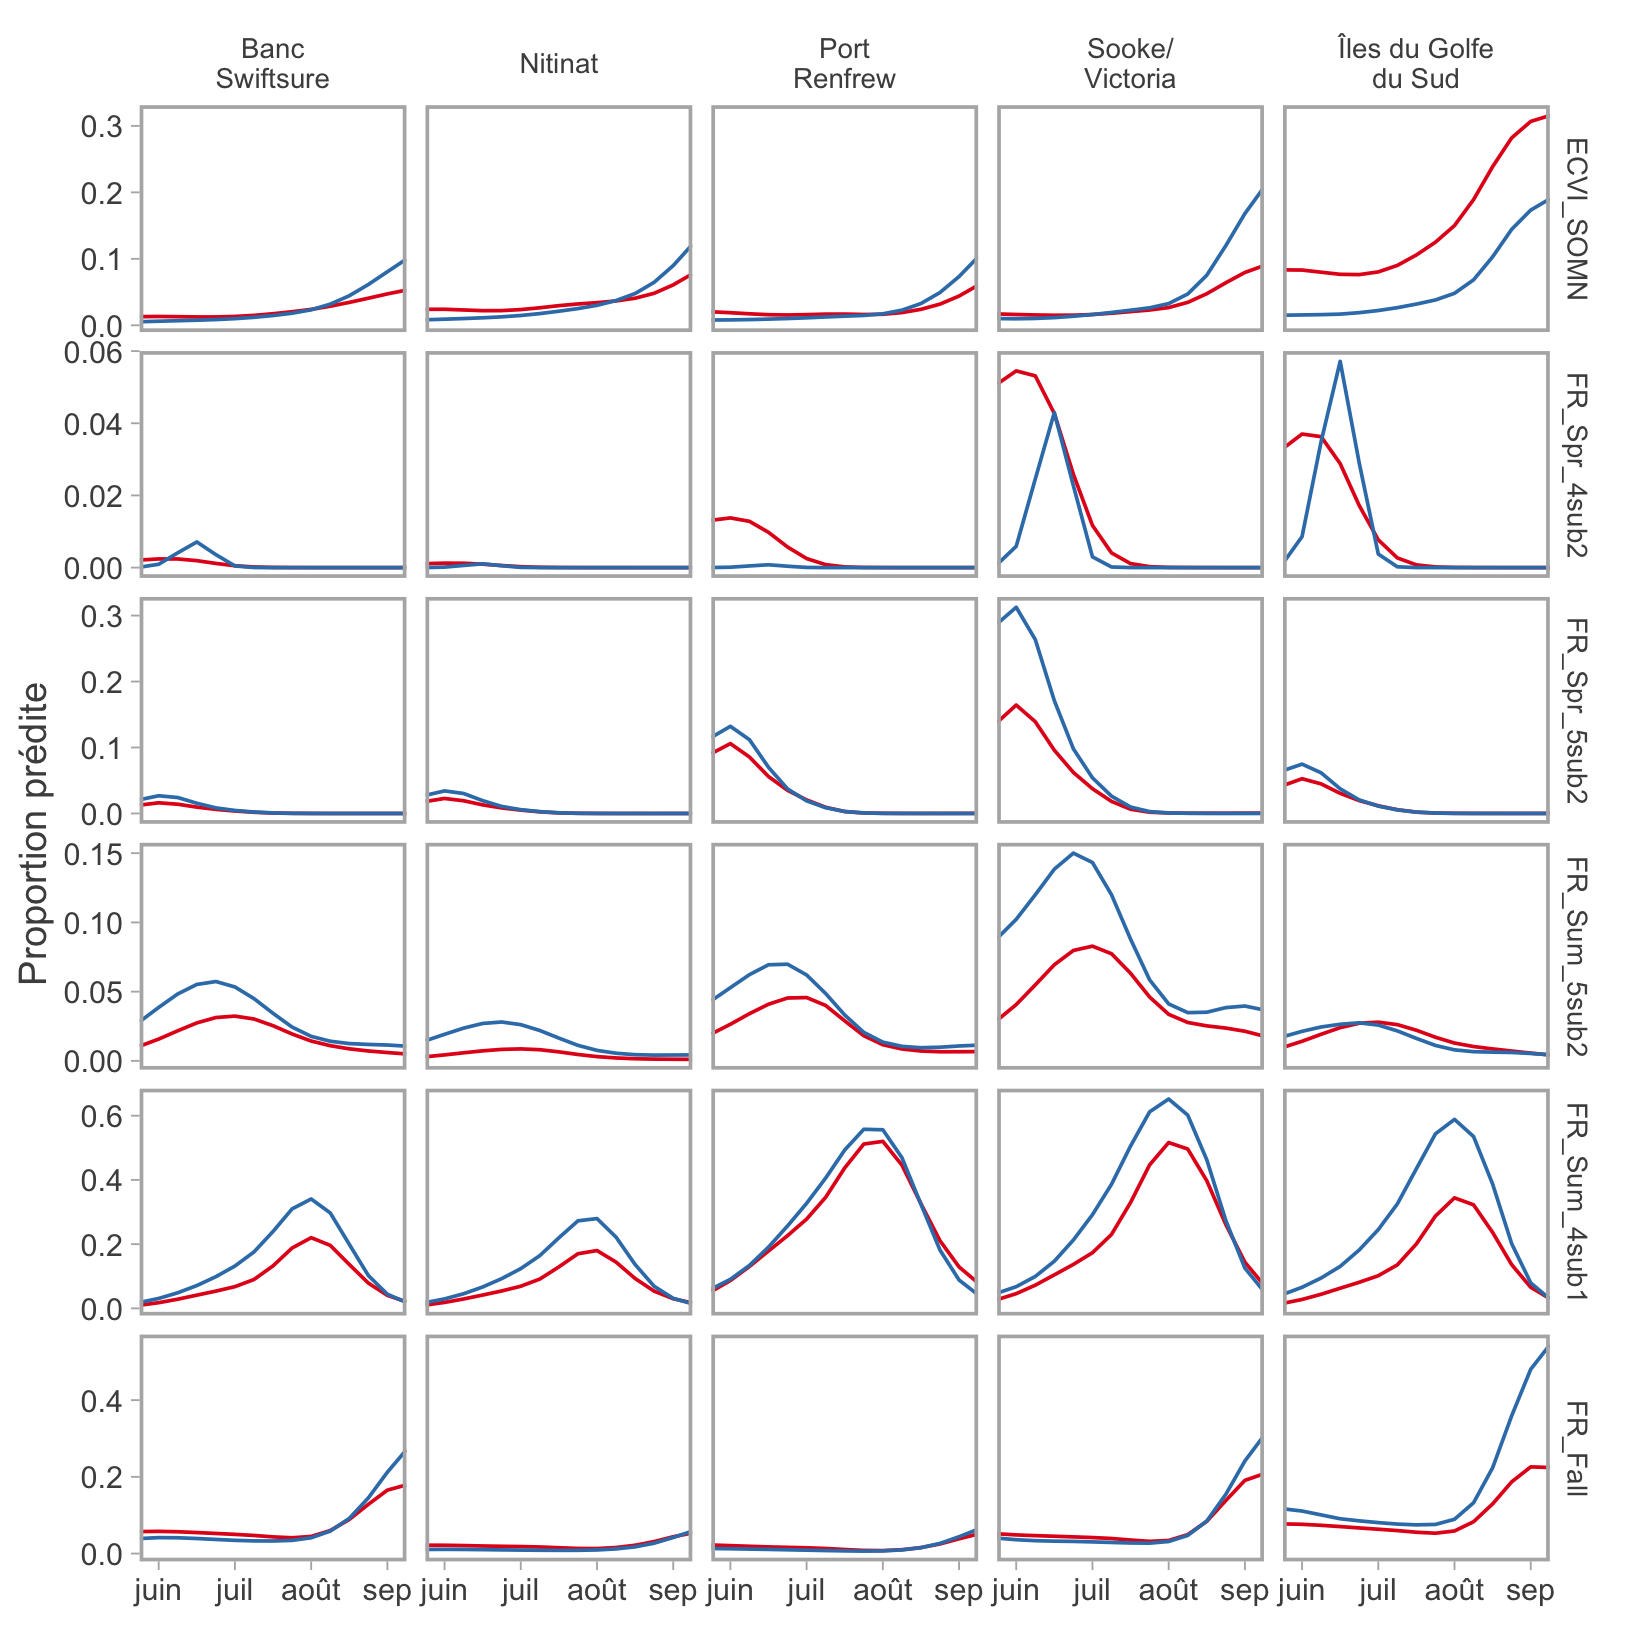
\includegraphics[width=5in]{figs/supp_figs/model_comp_stock2.png}}{Figure \ref{fig:comb-pred-stock2}}
    \caption{Prédictions saisonnières de l'abondance spécifique au stock pour les stocks ECVI/SOMN et du fleuve Fraser. Les prédictions sont basées sur le modèle standard présenté dans le texte principal (rouge), ainsi qu'un modèle ajusté uniquement aux données d'individus plus grands que 75 cm (bleu). Les prédictions représentent les estimations moyennes et les intervalles de confiance ne sont pas montrés pour améliorer la lisibilité. Notez les différences d'échelle de l'axe des y entre les stocks.}
    \label{fig:comb-pred-stock2}
\end{figure}

La composition simulée du modèle du scénario des grands individus était légèrement plus cohérente avec les restes de proies observés (Figure \ref{fig:comb-sel-stock}). Par exemple, la différence dans l'abondance proportionnelle des poissons de Puget Sound a diminué. Ces motifs suggèrent que la sélectivité de taille par les ERSN a contribué aux différences dans la composition du stock entre les prédictions du modèle et les échantillons observés. Néanmoins, ces différences étaient modestes et il y avait encore des preuves solides de surreprésentation pour les stocks Fraser River Summer $4_1$, Summer $5_2$ et Spring $5_2$, ainsi que de sous-représentation des stocks WCVI, Columbia River Summer/Fall et «\,Autre\,» (Figure \ref{fig:comb-sel-stock}). 

\begin{figure}[H]
    \centering
    \pdftooltip{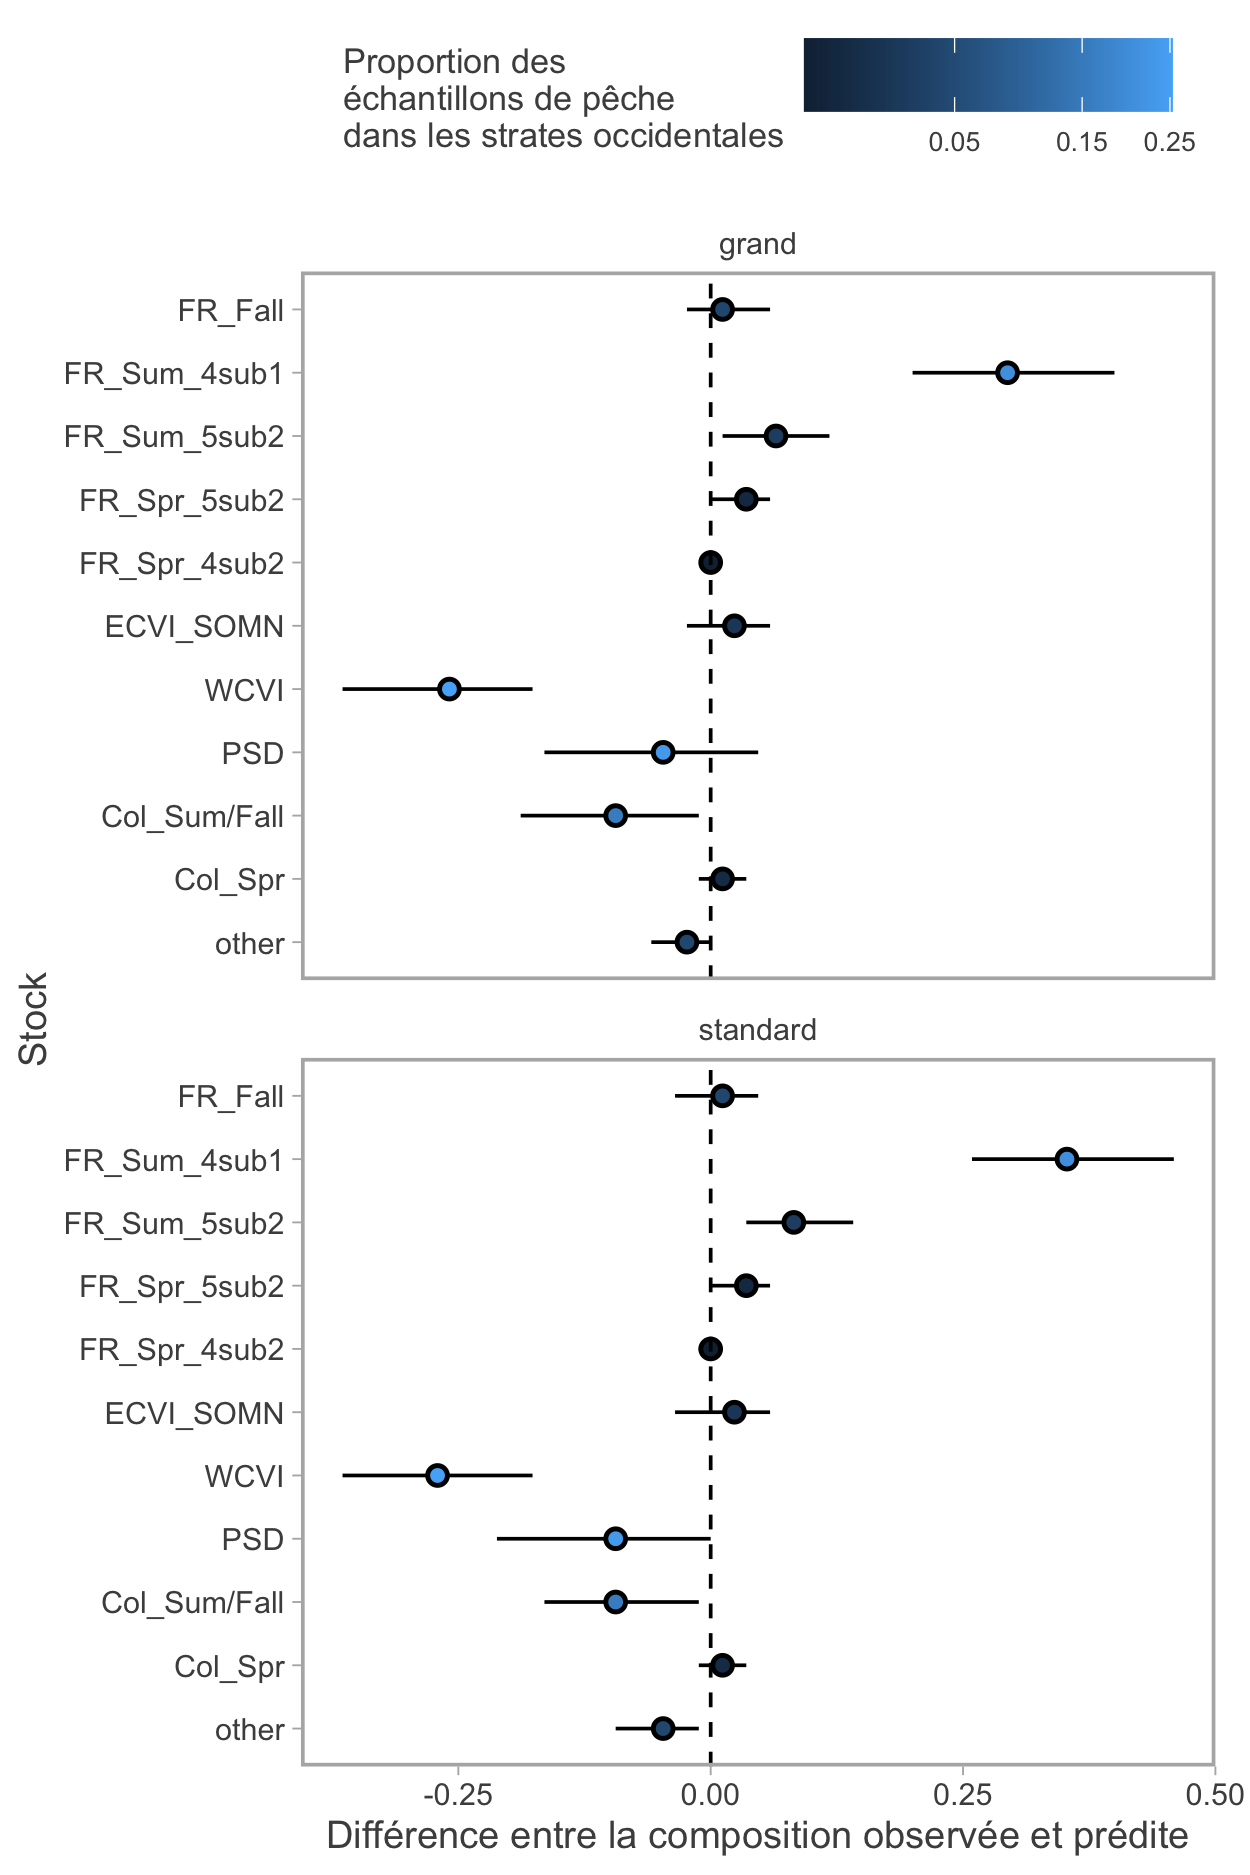
\includegraphics[width=5in]{figs/supp_figs/selectivity_bean_stock_comp.png}}{Figure \ref{fig:comb-sel-stock}}
    \caption{Différences entre la contribution observée et prédite par le modèle de chaque stock aux restes de proies des ERSN en utilisant le modèle standard présenté dans le texte principal (haut) et un modèle ajusté aux données excluant les individus plus petits que 75 cm de longueur à la fourche (bas). Les valeurs positives (négatives) indiquent qu'un stock donné a été observé plus (moins) fréquemment dans les restes de proies des ERSN que prédit par le modèle dépendant de la pêcherie. Les points représentent les médianes et les moustaches représentent les intervalles du 95e percentile parmi 500 simulations Monte Carlo. Les points plus lumineux (plus sombres) représentent les stocks qui étaient plus (moins) communs dans les échantillons de la pêche récréative des moments et strates coïncidant avec les restes de proies des ERSN.}
    \label{fig:comb-sel-stock}
\end{figure}

\appsection{Interventions de gestion}

Pour évaluer l'impact des interventions de gestion sur la sélectivité, nous avons retiré de la simulation les échantillons de proies qui ont été collectés pendant les moments et emplacements où les pêcheries coïncidentes étaient fermées ou impactées par les limites de taille maximales. 11 échantillons de proies ont été retirés de l'analyse de sélectivité du stock et huit ont été retirés de l'analyse de sélectivité de taille. Nous avons ensuite répété l'analyse de simulation et comparé les résultats aux résultats originaux présentés dans le texte principal.

Les estimations de sélectivité du stock (Figure \ref{fig:comb-sel-stock2}) et de taille (Figure \ref{fig:comb-sel-size2}) étaient qualitativement inchangées lorsqu'un ensemble plus conservateur de proies a été inclus dans la simulation. Ces résultats indiquent que la sélectivité du stock et de taille n'était pas uniquement motivée par la présence d'interventions de gestion. Cependant, il n'est pas possible de quantifier l'impact des interventions de gestion à travers la zone d'étude sur les estimations du modèle.

\begin{figure}[H]
    \centering
    \pdftooltip{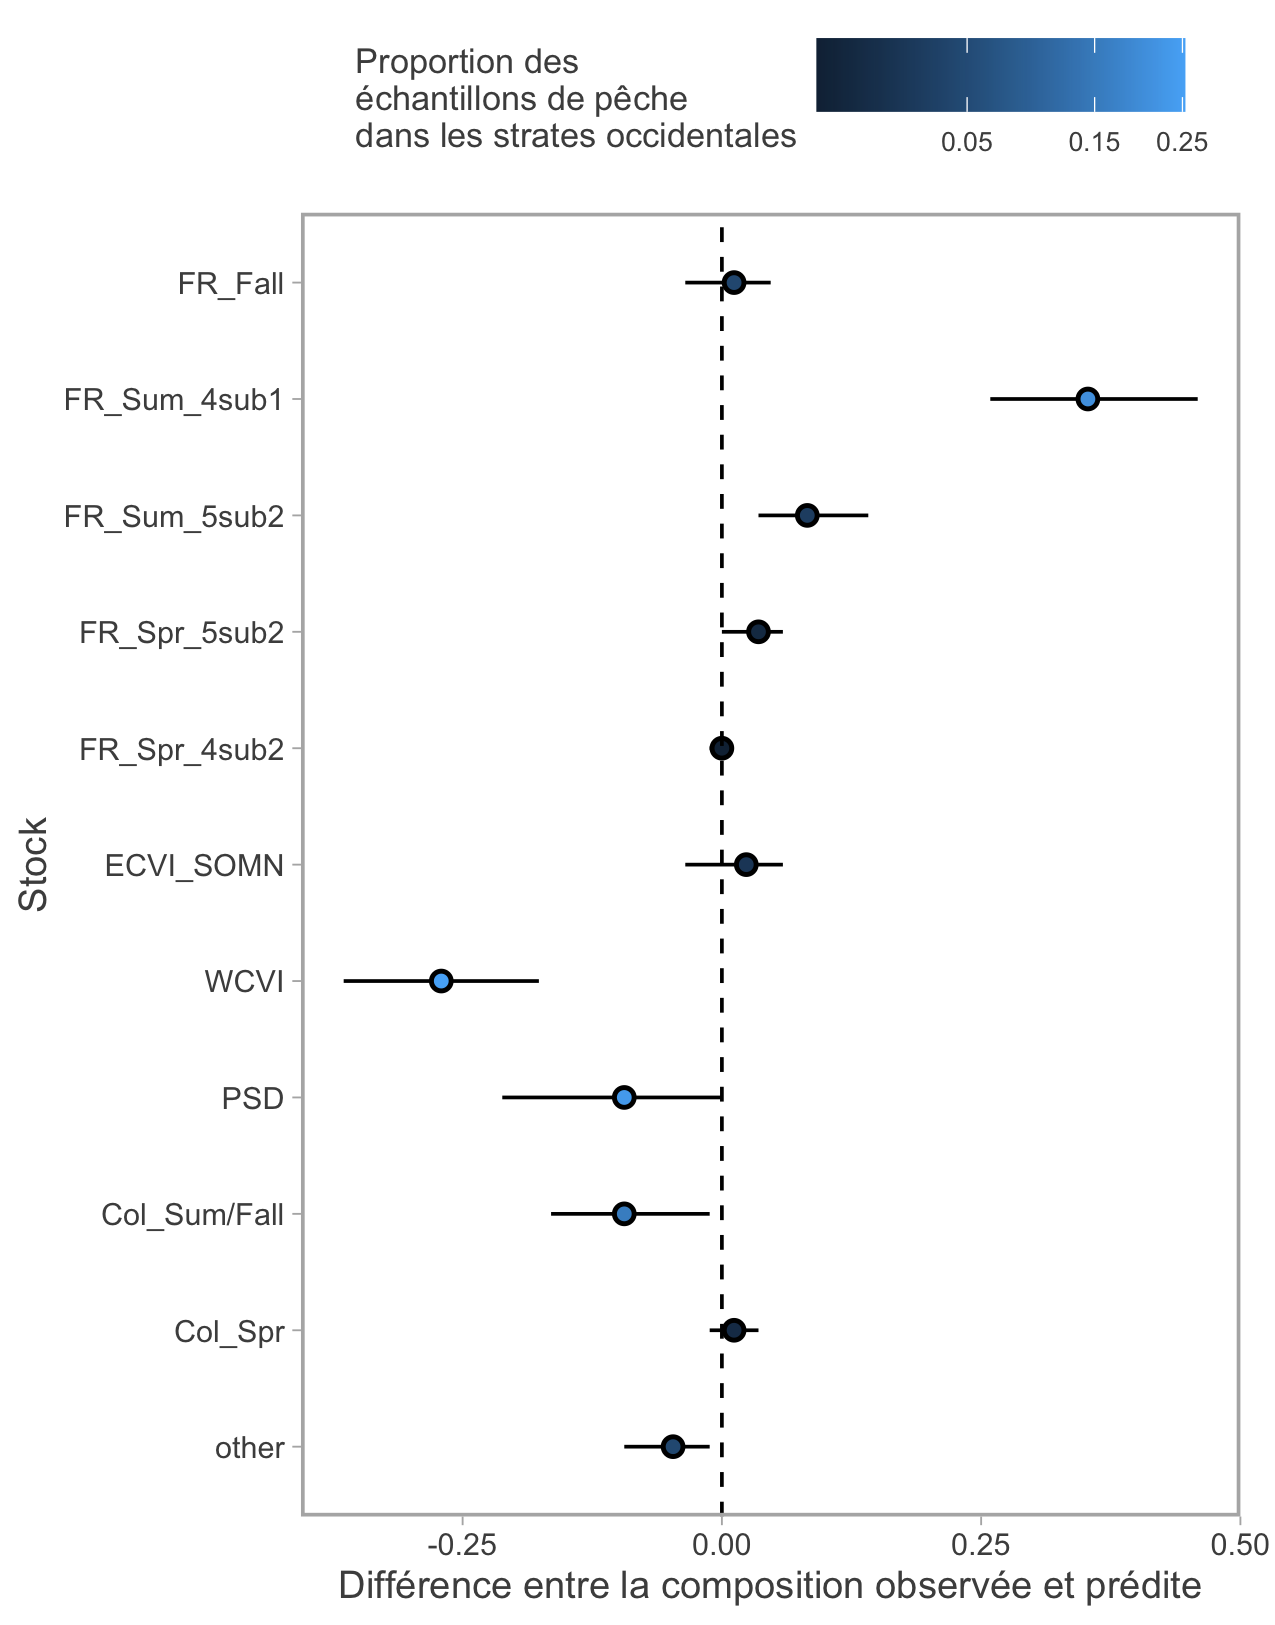
\includegraphics[width=5in]{figs/supp_figs/selectivity_bean_stock_sens.png}}{Figure \ref{fig:comb-sel-stock2}}
    \caption{Différences entre la contribution observée et prédite par le modèle de chaque stock aux restes de proies des ERSN en utilisant le jeu de données complet des restes de proies présenté dans le texte principal (haut) et les restes de proies qui ont exclu les échantillons collectés dans les moments et emplacements où les interventions de gestion étaient en place (bas). Les valeurs positives (négatives) indiquent qu'un stock donné a été observé plus (moins) fréquemment dans les restes de proies des ERSN que prédit par le modèle dépendant de la pêcherie. Les points représentent les médianes et les moustaches représentent les intervalles du 95e percentile parmi 500 simulations Monte Carlo. Les points plus lumineux (plus sombres) représentent les stocks qui étaient plus (moins) communs dans les échantillons de la pêche récréative des moments et strates coïncidant avec les restes de proies des ERSN.}
    \label{fig:comb-sel-stock2}
\end{figure}

\begin{figure}[H]
    \centering
    \pdftooltip{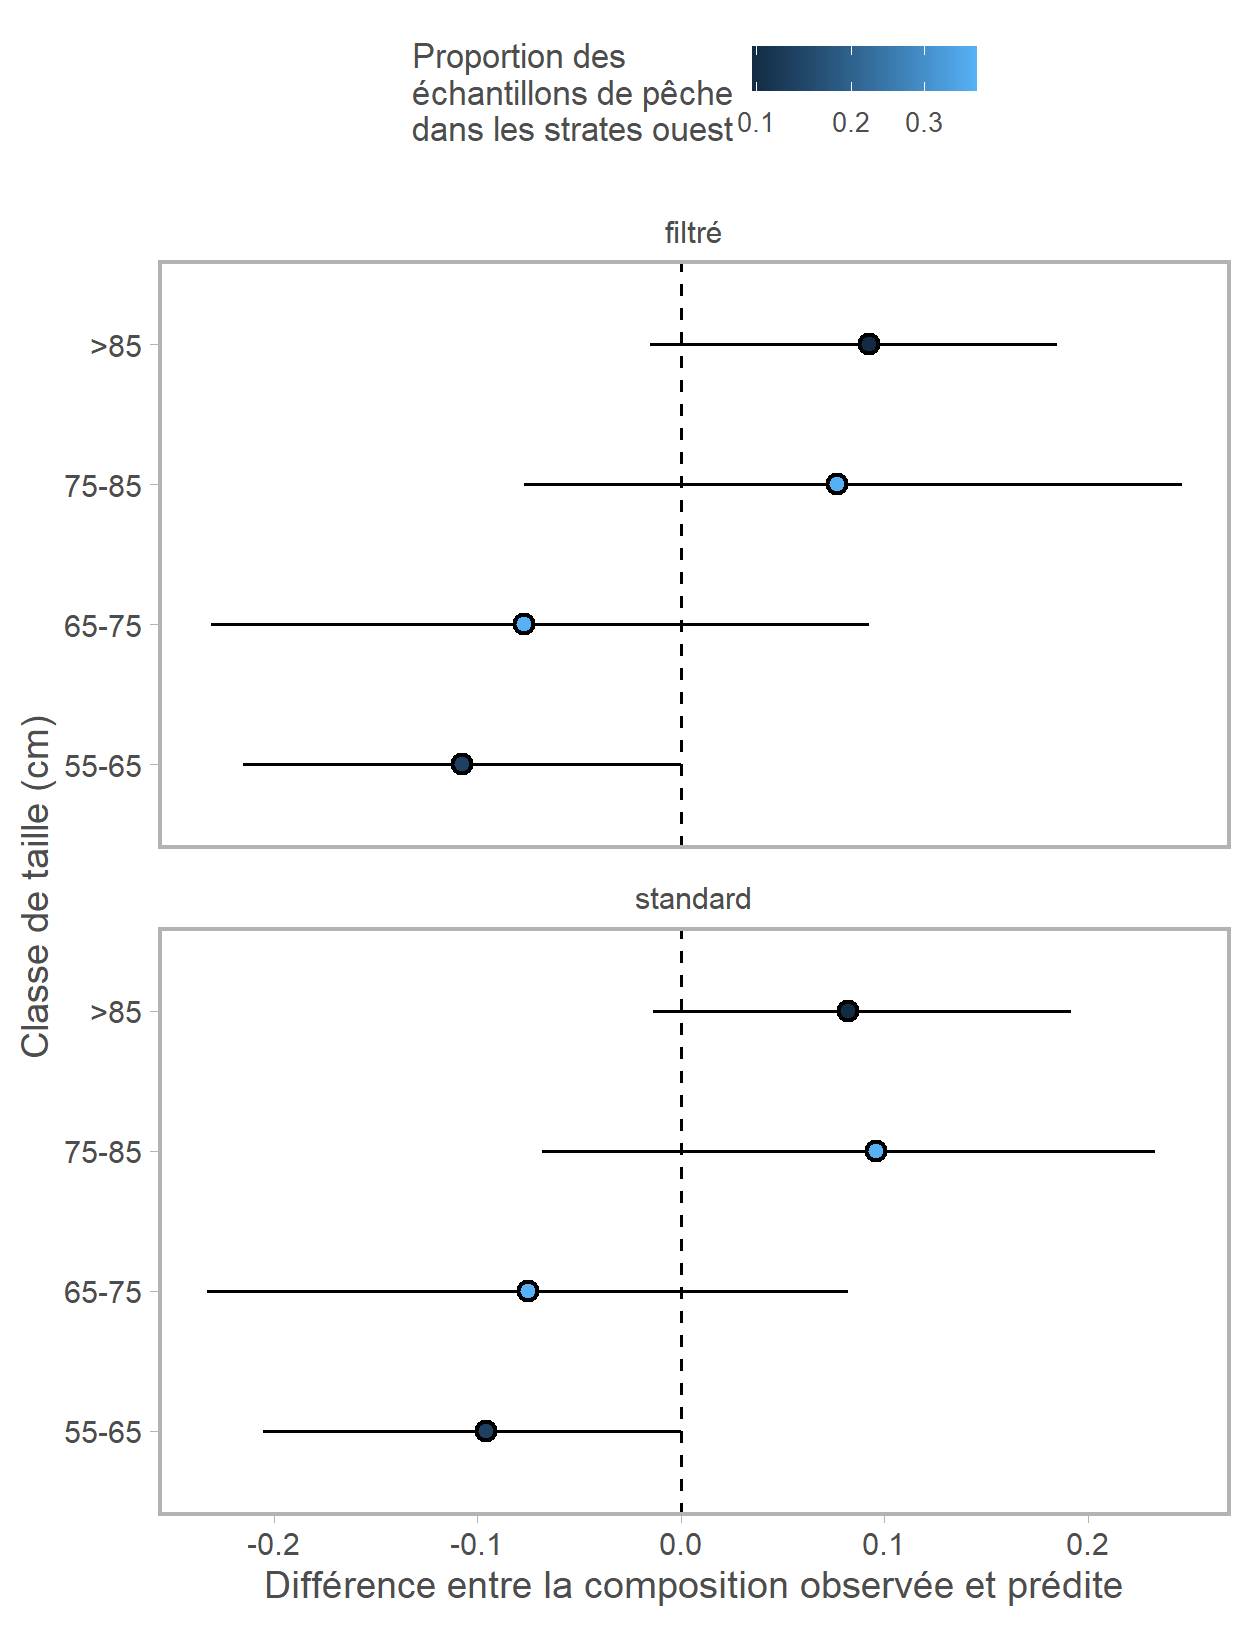
\includegraphics[width=5in]{figs/supp_figs/selectivity_bean_size_sens.png}}{Figure \ref{fig:comb-sel-size2}}
    \caption{Différences entre la contribution observée et prédite par le modèle de chaque classe de taille aux restes de proies des ERSN en utilisant le jeu de données complet des restes de proies présenté dans le texte principal (haut) et les restes de proies qui ont exclu les échantillons collectés dans les moments et emplacements où les interventions de gestion étaient en place (bas). Les valeurs positives (négatives) indiquent qu'une classe de taille donnée a été observée plus (moins) fréquemment dans les restes de proies des ERSN que prédit par le modèle dépendant de la pêcherie. Les points représentent les médianes et les moustaches représentent les intervalles du 95e percentile parmi 500 simulations Monte Carlo. Les points plus lumineux (plus sombres) représentent les classes de taille qui étaient plus (moins) communes dans les échantillons de la pêche récréative des moments et strates coïncidant avec les restes de proies des ERSN.}
    \label{fig:comb-sel-size2}
\end{figure}


\clearpage

\end{document}